\documentclass[12pt,a3paper]{article}
\usepackage{pgfplots}
%% ── Packages ──────────────────────────────────────────────────────────
\usepackage{amsmath,amssymb}
\usepackage{geometry}
\usepackage{enumitem}
\usepackage{titlesec}
\usepackage[hidelinks,colorlinks=true,linkcolor=blue!70!black]{hyperref}
\usepackage{xcolor}
\usepackage{fancyhdr}
\usepackage{tcolorbox}
\usepackage{multicol}
\usepackage{needspace}
\usepackage[strings]{underscore}
\usepackage{array,booktabs}
\usepackage[american]{circuitikz}
\usepackage{tikz}
\usepackage{multirow}
\pgfplotsset{compat=1.18}
\usepackage[table]{xcolor}

\usetikzlibrary{decorations.pathreplacing}
\usetikzlibrary{shapes.geometric}
\usetikzlibrary{circuits.logic.US, positioning, calc, arrows.meta, decorations.pathreplacing}

\tcbuselibrary{skins,breakable}
\geometry{margin=2.5cm,headheight=20pt,top=3cm,bottom=3cm}

%% ── Colors ────────────────────────────────────────────────────────────
\definecolor{pblue}{RGB}{13,71,161}
\definecolor{dgray}{RGB}{66,66,66}
\definecolor{cA}{RGB}{183,28,28}
\definecolor{cB}{RGB}{1,87,155}
\definecolor{cC}{RGB}{27,94,32}
\definecolor{cD}{RGB}{106,27,154}
\definecolor{cE}{RGB}{230,81,0}
\definecolor{cF}{RGB}{0,96,100}
\definecolor{cH}{RGB}{0,77,64}

%% ── Section headings ──────────────────────────────────────────────────
\titleformat{\section}{\large\bfseries\color{pblue}}{}{0em}{}[\titlerule]
\titleformat{\subsection}{\normalsize\bfseries}{}{0em}{}

%% ── Header / Footer ───────────────────────────────────────────────────
\pagestyle{fancy}\fancyhf{}
\renewcommand{\headrulewidth}{0.5pt}
\fancyhead[L]{\small\textcolor{pblue}{\textbf{BUET $|$ EEE 163 Question Bank}}}
\fancyhead[R]{\small\textcolor{dgray}{\itshape\nouppercase{\leftmark}}}
\fancyfoot[C]{\small\thepage}

%% ── Utility macros ────────────────────────────────────────────────────
\newcommand{\yr}[1]{\hfill\textcolor{gray}{\small\textbf{[#1]}}}
\newcommand{\mk}[1]{\textcolor{orange!70!black}{\small\textbf{(#1 marks)}}}
\newcommand{\variant}[1]{\par\vspace{1pt}\textcolor{blue!50!black}%
  {\footnotesize\itshape$\hookrightarrow$ Similar: #1}}
\newcommand{\diagram}{\par\vspace{4pt}\textcolor{gray!55}{\small\itshape[Diagram to be added manually]}}

%% ── Subtopic heading macro ────────────────────────────────────────────
\newcommand{\subtopic}[2]{%
  \vspace{10pt}
  \noindent\begin{tcolorbox}[colback=#1!8,colframe=#1,boxrule=0.6pt,arc=4pt,
    left=6pt,right=6pt,top=4pt,bottom=4pt]
    \small\bfseries\textcolor{#1}{#2}
  \end{tcolorbox}
  \vspace{2pt}
}

%% ── Section divider page ──────────────────────────────────────────────
\newcommand{\secdivider}[3]{%
  \newpage\thispagestyle{empty}%
  \vspace*{\fill}%
  \begin{tcolorbox}[enhanced,colback=#3!6,colframe=#3,boxrule=1.5pt,arc=8pt,
    left=20pt,right=20pt,top=22pt,bottom=22pt,
    shadow={3pt}{-3pt}{0pt}{black!15}]
    \centering
    {\large\textcolor{gray}{\textbf{EEE 163 $\cdot$ Introduction to Electrical Engineering}}}\\[8pt]
    {\fontsize{26}{32}\selectfont\bfseries\textcolor{#3}{Intro.\ to EEE}}\\[6pt]
    {\fontsize{15}{19}\selectfont\textcolor{dgray}{#1}}\\[12pt]
    \textcolor{#3!60}{\rule{0.5\textwidth}{0.5pt}}\\[6pt]
    {\small\textcolor{gray}{#2}}
  \end{tcolorbox}%
  \vspace*{\fill}\newpage%
}

%% ── List styles ───────────────────────────────────────────────────────
\setlist[enumerate,1]{label=\textbf{Q\arabic*.},leftmargin=*,itemsep=14pt,parsep=2pt}
\setlist[enumerate,2]{label=(\alph*),leftmargin=2em,itemsep=3pt}
\setlist[enumerate,3]{label=(\roman*),leftmargin=2.5em,itemsep=2pt}




\begin{document}

%% ══════════════════════════════════════════════════════════════════════
%%  COVER PAGE
%% ══════════════════════════════════════════════════════════════════════
\thispagestyle{empty}
\begin{tcolorbox}[enhanced,colback=pblue!5,colframe=pblue,boxrule=1.5pt,arc=6pt,
  top=28pt,bottom=28pt,left=22pt,right=22pt,
  shadow={4pt}{-4pt}{0pt}{black!20}]
  \centering

  % --- BUET Logo Added Here ---
  
\includegraphics[height=2.5cm]{images/buet_logo.png}\\[8pt]
  % ----------------------------

  {\Large\bfseries\textcolor{pblue}{Bangladesh University of Engineering and Technology}}\\[4pt]
  {\normalsize\textcolor{dgray}{Department of Computer Science \& Engineering}}\\[18pt]
  \textcolor{pblue}{\rule{\textwidth}{1pt}}\\[14pt]

  {\fontsize{22}{28}\selectfont\bfseries\textcolor{pblue}{Introduction to Electrical Engineering Question Bank}}\\[8pt]
  {\fontsize{14}{18}\selectfont\textcolor{dgray}{EEE 163 $\cdot$ Introduction to Electrical Engineering}}\\[4pt]
  \textcolor{pblue}{\rule{\textwidth}{0.5pt}}\\[14pt]

  {\small\textcolor{dgray}{Year Coverage: 2005--06 to 2024--25\\Topics: Direct Current, Network Theorems, Alternating Current,\\
  RLC Circuits, Phasor Analysis, Three-Phase Circuits, Filters \& Op-Amps}}\\[16pt]

    {\small\bfseries\textcolor{dgray}{Authors \& Contributors}}\\[6pt]
    \begin{tabular}{rl}
      \textcolor{dgray}{\textbf{Md Ratul Hasan}} \textcolor{dgray}{\small(2405009)} & --- Question Curation \& Organisation\\
      & --- \LaTeX\ Typesetting\\[3pt]
      \textbf{NotebookLM} & --- Research \& Extraction\\[3pt]
      \textbf{Claude AI}  & --- \LaTeX\ Typesetting\\[3pt]
      \textbf{Gemini}     & --- Diagram Generation\\[3pt]
    \end{tabular}
\end{tcolorbox}
\newpage

%% ══════════════════════════════════════════════════════════════════════
%%  TABLE OF CONTENTS
%% ══════════════════════════════════════════════════════════════════════
\thispagestyle{fancy}\markboth{Table of Contents}{}
\begin{center}
  {\LARGE\bfseries\textcolor{pblue}{Table of Contents}}\\[6pt]
  \textcolor{pblue}{\rule{0.6\textwidth}{0.8pt}}
\end{center}
\vspace{6pt}

%% Part I
\begin{tcolorbox}[breakable,colback=cA!5,colframe=cA,boxrule=1pt,arc=5pt,
  left=8pt,right=8pt,top=8pt,bottom=8pt,before skip=4pt]
  {\large\bfseries\textcolor{cA}{Part I --- Direct Current (DC) Circuits}}\\[5pt]
  \textcolor{cA!40}{\rule{\textwidth}{0.4pt}}\\[3pt]
  \small\begin{itemize}[leftmargin=1.2em,itemsep=1pt,label={\textcolor{cA}{$\triangleright$}}]
    \item \hyperref[sec:S1]{\textbf{S1.} DC Circuit Fundamentals}
      \begin{itemize}[leftmargin=1.5em,itemsep=0pt,label={\textcolor{cA}{$\cdot$}}]
        \item \hyperref[sub:s1-resistance]{Resistance \& Equivalent Resistance}
        \item \hyperref[sub:s1-circuit]{Circuit Analysis (KVL/KCL)}
        \item \hyperref[sub:s1-mesh]{Mesh / Loop Analysis}
        \item \hyperref[sub:s1-nodal]{Nodal Analysis}
        \item \hyperref[sub:s1-theorems]{Network Theorems (Superposition, Thevenin, Norton, MPT)}
      \end{itemize}
  \end{itemize}
\end{tcolorbox}

\vspace{6pt}

%% Part II
\begin{tcolorbox}[breakable,colback=cB!5,colframe=cB,boxrule=1pt,arc=5pt,
  left=8pt,right=8pt,top=8pt,bottom=8pt,before skip=4pt]
  {\large\bfseries\textcolor{cB}{Part II --- Alternating Current (AC) Circuits}}\\[5pt]
  \textcolor{cB!40}{\rule{\textwidth}{0.4pt}}\\[3pt]
  \small\begin{itemize}[leftmargin=1.2em,itemsep=1pt,label={\textcolor{cB}{$\triangleright$}}]
    \item \hyperref[sec:S2]{\textbf{S2.} AC Fundamentals \& RLC Circuits}
      \begin{itemize}[leftmargin=1.5em,itemsep=0pt,label={\textcolor{cB}{$\cdot$}}]
        \item \hyperref[sub:s2-rms]{RMS \& Average Values}
        \item \hyperref[sub:s2-sinusoidal]{Sinusoidal Signals \& Phasors}
        \item \hyperref[sub:s2-rl]{RL Circuits}
        \item \hyperref[sub:s2-rc]{RC Circuits}
        \item \hyperref[sub:s2-rlc]{RLC Circuits}
        \item \hyperref[sub:s2-power]{Power in AC Circuits}
        \item \hyperref[sub:s2-phasor]{Phasor Diagrams}
        \item \hyperref[sub:s2-circuit]{AC Circuit Analysis}
      \end{itemize}
  \end{itemize}
\end{tcolorbox}

\vspace{6pt}

%% Part III
\begin{tcolorbox}[breakable,colback=cC!5,colframe=cC,boxrule=1pt,arc=5pt,
  left=8pt,right=8pt,top=8pt,bottom=8pt,before skip=4pt]
  {\large\bfseries\textcolor{cC}{Part III --- Three-Phase Circuits}}\\[5pt]
  \textcolor{cC!40}{\rule{\textwidth}{0.4pt}}\\[3pt]
  \small\begin{itemize}[leftmargin=1.2em,itemsep=1pt,label={\textcolor{cC}{$\triangleright$}}]
    \item \hyperref[sec:S3]{\textbf{S3.} Three-Phase Systems}
      \begin{itemize}[leftmargin=1.5em,itemsep=0pt,label={\textcolor{cC}{$\cdot$}}]
        \item \hyperref[sub:s3-threephasepower]{Three-Phase Power \& Power Factor}
        \item \hyperref[sub:s3-star]{Star (Wye) Connection}
        \item \hyperref[sub:s3-delta]{Delta Connection}
      \end{itemize}
  \end{itemize}
\end{tcolorbox}

\vspace{6pt}

%% Part IV
\begin{tcolorbox}[breakable,colback=cE!5,colframe=cE,boxrule=1pt,arc=5pt,
  left=8pt,right=8pt,top=8pt,bottom=8pt,before skip=4pt]
  {\large\bfseries\textcolor{cE}{Part IV --- Filters \& Operational Amplifiers}}\\[5pt]
  \textcolor{cE!40}{\rule{\textwidth}{0.4pt}}\\[3pt]
  \small\begin{itemize}[leftmargin=1.2em,itemsep=1pt,label={\textcolor{cE}{$\triangleright$}}]
    \item \hyperref[sec:S4]{\textbf{S4.} Filters \& Op-Amp Circuits}
      \begin{itemize}[leftmargin=1.5em,itemsep=0pt,label={\textcolor{cE}{$\cdot$}}]
        \item \hyperref[sub:s4-lowpass]{Low-pass Filters}
        \item \hyperref[sub:s4-filters]{Band-pass Filters}
        \item \hyperref[sub:s4-resonance]{Frequency Response \& Resonance}
        \item \hyperref[sub:s4-opamp]{Op-Amp Applications}
        \item \hyperref[sub:s4-math]{Op-Amp Mathematical Circuits}
      \end{itemize}
  \end{itemize}
\end{tcolorbox}

\vspace{6pt}

%% Part V
\begin{tcolorbox}[breakable,colback=cD!5,colframe=cD,boxrule=1pt,arc=5pt,
  left=8pt,right=8pt,top=8pt,bottom=8pt,before skip=4pt]
  {\large\bfseries\textcolor{cD}{Part V --- Magnetic Circuits}}\\[5pt]
  \textcolor{cD!40}{\rule{\textwidth}{0.4pt}}\\[3pt]
  \small\begin{itemize}[leftmargin=1.2em,itemsep=1pt,label={\textcolor{cD}{$\triangleright$}}]
    \item \hyperref[sec:S5]{\textbf{S5.} Magnetic Circuits}
      \begin{itemize}[leftmargin=1.5em,itemsep=0pt,label={\textcolor{cD}{$\cdot$}}]
        \item \hyperref[sub:s5-magnetic]{Magnetic Circuit Analysis}
        \item \hyperref[sub:s5-hysteresis]{Hysteresis \& Magnetic Properties}
      \end{itemize}
  \end{itemize}
\end{tcolorbox}

\vspace{6pt}

%% Part VI
\begin{tcolorbox}[breakable,colback=cF!5,colframe=cF,boxrule=1pt,arc=5pt,
  left=8pt,right=8pt,top=8pt,bottom=8pt,before skip=4pt]
  {\large\bfseries\textcolor{cF}{Part VI --- Miscellaneous \& Short Notes}}\\[5pt]
  \textcolor{cF!40}{\rule{\textwidth}{0.4pt}}\\[3pt]
  \small\begin{itemize}[leftmargin=1.2em,itemsep=1pt,label={\textcolor{cF}{$\triangleright$}}]
    \item \hyperref[sec:S6]{\textbf{S6.} Miscellaneous \& Short Notes}
      \begin{itemize}[leftmargin=1.5em,itemsep=0pt,label={\textcolor{cF}{$\cdot$}}]
        \item \hyperref[sub:s6-shortnotes]{Short Notes}
      \end{itemize}
  \end{itemize}
\end{tcolorbox}

\newpage


%% ══════════════════════════════════════════════════════════════════════
%%  PART I
%% ══════════════════════════════════════════════════════════════════════
\secdivider{Part I --- Direct Current (DC) Circuits}{Resistance, KVL/KCL, Mesh Analysis, Nodal Analysis, Superposition, Thevenin, Norton \& Maximum Power Transfer}{cA}

%% ══════════════════════════════════════════════════════════════════════
%%  SECTION 1: DC CIRCUIT FUNDAMENTALS
%% ══════════════════════════════════════════════════════════════════════
\markboth{S1: DC Circuit Fundamentals}{S1: DC Circuit Fundamentals}
\label{sec:S1}
\titleformat{\section}{\large\bfseries\color{cA}}{}{0em}{}[\titlerule]
\section*{S1 \quad DC Circuit Fundamentals}
\addcontentsline{toc}{section}{S1: DC Circuit Fundamentals}

%%──────────────────────────────────────────────────────────────────────
\subtopic{cA}{Resistance \& Equivalent Resistance}
\label{sub:s1-resistance}

\begin{enumerate}
  
\item For the combination of resistors shown below, find the equivalent resistance $R_{ab}$.
\begin{center}
  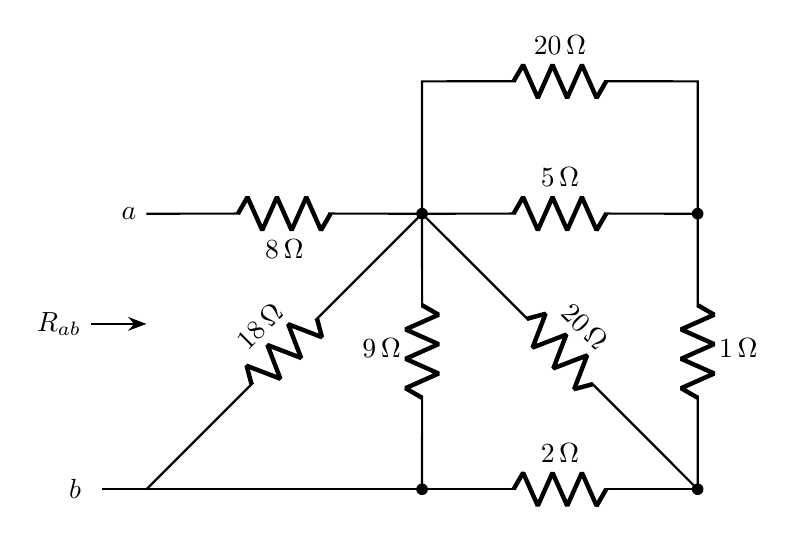
\begin{tikzpicture}[thick, american, scale=1.4]
    
    % Input terminals a and b
    \node[left] at (0,2.5) {$a$};
    \node[left] at (-0.5,0) {$b$};
    
    % Defining main wire junctions
    % Central star junction node: (2.5, 2.5)
    % Bottom-right corner node: (5, 0)
    % Middle-right node: (5, 2.5)
    
    % Branch from terminal 'a' to the central star junction
    \draw (2.5,2.5) to[R, l=$8\,\Omega$] (0,2.5);
    
    % Bottom node connection line from terminal 'b'
    \draw (-0.4,0) -- (2.5,0);
    
    % Diagonal resistor from node 'b' up to the central junction
    \draw (0,0) to[R, l=$18\,\Omega$] (2.5,2.5);
    
    % Vertical resistor from bottom wire up to the central junction
    \draw (2.5,0) to[R, l=$9\,\Omega$] (2.5,2.5);
    
    % Diagonal resistor down to the bottom-right corner from the central junction
    \draw (2.5,2.5) to[R, l=$20\,\Omega$] (5,0);
    
    % Bottom-right resistor along the baseline
    \draw (2.5,0) to[R, l=$2\,\Omega$] (5,0);
    
    % First horizontal resistor between central junction and middle-right node
    \draw (2.5,2.5) to[R, l=$5\,\Omega$] (5,2.5);
    
    % Upper parallel path loop containing the 20 ohm resistor
    \draw (2.5,2.5) -- (2.5,3.7) 
                    to[R, l=$20\,\Omega$] (5,3.7) 
                    -- (5,2.5);
                    
    % Vertical resistor on the right side connecting middle-right to bottom-right
    \draw (5,2.5) to[R, l=$1\,\Omega$] (5,0);

    % Central junction point dot
    \fill (2.5,2.5) circle (1.5pt);
    \fill (2.5,0) circle (1.5pt);
    \fill (5,2.5) circle (1.5pt);
    \fill (5,0) circle (1.5pt);
    
    % Optional indicator arrow for Rab
    \draw[-{Stealth}, thick] (-0.5,1.5) -- (0,1.5) node[left, pos=0] {$R_{ab}$};

\end{tikzpicture}

\end{center}
\mk{10} \yr{EEE 163 | L-1/T-1 | 2020--21}

\item Find the resistance shown across terminal c--d ($R_{cd}$) for the circuit below.
  \begin{center}
    \begin{circuitikz}[thick,american, x=1.5cm  , y=1.5cm, transform shape]

    % --- Define 3D Cube Node Coordinates ---
    % Front Face Corners
    \coordinate (F_BL) at (3,0);       % Bottom Left
    \coordinate (F_BR) at (6,0);       % Bottom Right
    \coordinate (F_TL) at (3,3);       % Top Left
    \coordinate (F_TR) at (6,3);       % Top Right

    % Back Face Corners (Shifted up and right using an oblique offset vector)
    \coordinate (B_BL) at (1,1);       % Bottom Left
    \coordinate (B_BR) at (4,1);       % Bottom Right
    \coordinate (B_TL) at (1,4);       % Top Left
    \coordinate (B_TR) at (4,4);       % Top Right

    % --- 1. Draw Inner Cube Resistors & Connecting Structural Lines ---
    % Front Face Edges (Resistors)
    \draw (F_BL) -- (F_BR) to[R, l=$20\Omega$] (8,0)node[ocirc, label=below:$d$] {};
    \draw (F_BL) to[R, l_=$52\Omega$] (F_TL);
    \draw (F_TL) to[R, l_=$20\Omega$] (F_TR);
    \draw (F_BR) -- (F_TR);

    % Back Face Edges (Resistors)
    \draw (B_BL) to[R, l=$10\Omega$] (1,2.5) to[R, l=$10\Omega$] (B_TL);
    \draw (B_TL) to[R, l=$30\Omega$] (B_TR) to[R, l=$10\Omega$] (6,4) node[ocirc, label=below:$c$] {};
    \draw (1,2.5) to[R, l_=$40\Omega$] (F_TL);
    \draw (1,2.5) to[R, l=$60\Omega$] (F_BL);


    % Front-to-Back Interconnecting Edges (Resistors)
    \draw (F_BL) to[R, l=$30\Omega$] (B_BL);
    \draw (F_TL) to[R, l=$50\Omega$] (B_TL);
    \draw (F_TR) to[R, l=$10\Omega$] (B_TR);



    % Rightmost External Resistor Loop
    % \draw (B_TR) -- (5.2,4) to[R, l=$R$] (5.2,1) -- (B_BR);

    % --- 3. Input/Output Terminals & Probes ---
    % Node A (Top-Left input line)
    \draw (B_TL) to[R, l=$33\Omega$] (-1.5,4) node[ocirc, label=below:$a$] {};
    
    % Node B (Bottom-Left ground reference line)
    \draw (B_BL) to[R, l=$40\Omega$] (-1.5,1) node[ocirc, label=below left:$b$] {};
    



\end{circuitikz}
  \end{center}
\mk{18} \yr{EEE 163 | L-1/T-1 | 2018--19, 2015--16}

\item Find the equivalent resistance between terminals `a' and `b' in the circuit shown below.
\begin{center}
  \begin{circuitikz}[y=1.4cm , x=1.4cm , thick]

    % =========================================================================
    % 1. INNER RING (Concentric inner square)
    % =========================================================================
    % Defining corner nodes for the inner loop
    \coordinate (InTL) at (2,4);
    \coordinate (InTR) at (5,4);
    \coordinate (InBL) at (2,1);
    \coordinate (InBR) at (5,1);
    
    % Midpoints of the inner square for connection injections
    \coordinate (InTopMid) at (3.5,4);
    \coordinate (InLeftMid) at (2,2.5);
    \coordinate (InBotMid) at (3.5,1);

    % Top side of inner loop
    \draw (InTL) to[R, l=$40\,\Omega$] (InTopMid)
                to[R, l=$80\,\Omega$] (InTR);
                
    % Right side of inner loop
    \draw (InTR) to[R, l=$40\,\Omega$] (InBR);
    
    % Bottom side of inner loop
    \draw (InBR) to[R, l=$80\,\Omega$] (InBotMid)
                to[R, l=$40\,\Omega$] (InBL);
                
    % Left side of inner loop
    \draw (InBL) to[R, l=$40\,\Omega$] (InLeftMid)
                to[R, l=$40\,\Omega$] (InTL);


    % =========================================================================
    % 2. OUTER RING (Concentric outer square)
    % =========================================================================
    % Defining corner nodes for the outer loop
    \coordinate (OutTL) at (0,5);
    \coordinate (OutTR) at (7,5);
    \coordinate (OutBL) at (0,0);
    \coordinate (OutBR) at (7,0);
    
    % Midpoints of the outer square
    \coordinate (OutTopMid) at (3.5,5);
    \coordinate (OutLeftMid) at (0,2.5);
    \coordinate (OutBotMid) at (3.5,0);

    % Top side of outer loop
    \draw (OutTL) to[short] (OutTopMid)
                 to[R, l=$80\,\Omega$] (OutTR);
                 
    % Right side of outer loop
    \draw (OutTR) to[R, l=$120\,\Omega$] (OutBR);
    
    % Bottom side of outer loop
    \draw (OutBR) to[short] (OutBL);
    
    % Left side of outer loop split by two resistors
    \draw (OutBL) to[R, l=$80\,\Omega$] (OutLeftMid)
                 to[R, l=$80\,\Omega$] (OutTL);


    % =========================================================================
    % 3. INTER-RING CROSS CONNECTIONS & INNER TERMINALS (a, b)
    % =========================================================================
    % Top bridging line connecting outer top to inner top
    \draw (OutTopMid) to[short, -*] (InTopMid);
    
    % Center-left bridge resistor
    \draw (OutLeftMid) to[R, l=$80\,\Omega$, -*] (InLeftMid);
    
    % Bottom bridging line connecting outer bottom to inner bottom
    \draw (OutBotMid) to[short, -*] (InBotMid);

    % Terminal 'a' branching down from the top inner junction midpoint
    \draw (InTopMid) to[short, -o] (3.5,3.2) node[left] {a};

    % Terminal 'b' branching up from the bottom inner junction midpoint
    \draw (InBotMid) to[short, -o] (3.5,1.8) node[left] {b};
    \draw (InTR) -- (7,4);

\end{circuitikz}

\end{center}
\mk{15} \yr{EEE 163 | L-1/T-1 | 2018--19}

\item Find the equivalent resistance $R_{ab}$ in the circuit below.
\begin{center}
  \begin{circuitikz}[thick , scale=1.5]
    % --- Coordinate Definitions ---
    % Top Rail
    \coordinate (A) at (0,4);
    \coordinate (TM) at (4,4);
    \coordinate (TR) at (8,4);
    
    % Middle Axis
    \coordinate (ML) at (0,2);
    \coordinate (C1) at (2,2);
    \coordinate (C2) at (6,2);
    \coordinate (MR) at (8,2);
    
    % Bottom Rail
    \coordinate (B) at (0,0);
    \coordinate (BM) at (4,0);
    \coordinate (BR) at (8,0);
    
    % --- Input Terminals ---
    \draw (-0.7,4) node[left] {a} to[short, o-] (A);
    \draw (-0.7,0) node[left] {b} to[short, o-] (B);
    
    % --- Main Rails (Wires) ---
    \draw (A) -- (TM) -- (TR);
    \draw (B) -- (BM) -- (BR);
    
    % --- Vertical Resistor Columns ---
    \draw (A) to[R, l=$R$] (ML) to[R, l=$R$] (B);
    \draw (TR) to[R, l=$R$] (MR) to[R, l=$R$] (BR);
    
    % --- Middle Horizontal Resistors ---
    \draw (ML) to[R, l=$R$] (C1) to[R, l=$R$] (C2) to[R, l=$R$] (MR);
    
    % --- Diagonal Resistors (Left Fan) ---
    \draw (A) to[R, l=$R$] (C1);
    \draw (B) to[R, l=$R$] (C1);
    
    % --- Diagonal Resistors (Middle Diamond) ---
    \draw (C1) to[R, l=$R$] (TM);
    \draw (C1) to[R, l=$R$] (BM);
    \draw (TM) to[R, l=$R$] (C2);
    \draw (BM) to[R, l=$R$] (C2);
    
    % --- Diagonal Resistors (Right Fan) ---
    \draw (C2) to[R, l=$R$] (TR);
    \draw (C2) to[R, l=$R$] (BR);
    
    % --- Junction Dots ---
    \foreach \n in {A, TM, TR, ML, C1, C2, MR, B, BM, BR}
        \fill (\n) circle (2pt);
        
    \draw[->, thick] (-0.9, 2.0) -- (-0.4, 2.0);
    \node[below] at (-0.9, 1.4) {$R_{ab}$};

\end{circuitikz}

\end{center}
\mk{10} \yr{EEE 163 | L-1/T-1 | 2017--18}


\item Find the equivalent resistance between terminal `a' and `b' in the circuit shown below.(R=$5\Omega$)
  \begin{center}
    \begin{circuitikz}[thick,american, x=1.5cm  , y=1.5cm, transform shape]

    % --- Define 3D Cube Node Coordinates ---
    % Front Face Corners
    \coordinate (F_BL) at (0,0);       % Bottom Left
    \coordinate (F_BR) at (3,0);       % Bottom Right
    \coordinate (F_TL) at (0,3);       % Top Left
    \coordinate (F_TR) at (3,3);       % Top Right

    % Back Face Corners (Shifted up and right using an oblique offset vector)
    \coordinate (B_BL) at (1,1);       % Bottom Left
    \coordinate (B_BR) at (4,1);       % Bottom Right
    \coordinate (B_TL) at (1,4);       % Top Left
    \coordinate (B_TR) at (4,4);       % Top Right

    % --- 1. Draw Inner Cube Resistors & Connecting Structural Lines ---
    % Front Face Edges (Resistors)
    \draw (F_BL) to[R, l=$4R$] (F_BR);
    \draw (F_BL) to[R, l=$2R$] (F_TL);
    \draw (F_TL) to[R, l=$R$] (F_TR);
    \draw (F_BR) to[R, l=$2R$] (F_TR);

    % Back Face Edges (Resistors)
    \draw (B_BL) to[R, l=$4R$] (B_BR);
    \draw (B_BL) to[R, l=$2R$] (B_TL);
    \draw (B_TL) to[R, l=$R$] (B_TR);
    \draw (B_BR) to[R, l=$2R$] (B_TR);

    % Front-to-Back Interconnecting Edges (Resistors)
    \draw (F_BL) -- (B_BL);
    \draw (F_BR) -- (B_BR);
    \draw (F_TL) to[R, l=$R$] (B_TL);
    \draw (F_TR) to[R, l=$R$] (B_TR);



    % Rightmost External Resistor Loop
    % \draw (B_TR) -- (5.2,4) to[R, l=$R$] (5.2,1) -- (B_BR);

    % --- 3. Input/Output Terminals & Probes ---
    % Node A (Top-Left input line)
    \draw (B_TL) -- (-1.5,4) node[ocirc, label=below:$A$] {};
    
    % Node B (Bottom-Left ground reference line)
    \draw (F_BL) -- (-1.5,0) node[ocirc, label=below left:$B$] {};
    
    % Req Arrow Indicator on the left side
    \draw[->, thick] (-2, 0.5) -- (-1.7, 0.5) -- (-1.7, 1.2);
    \node[left] at (-1.8, 0.5) {$R_{eq}$};


\end{circuitikz}
  \end{center}
\mk{18} \yr{EEE 163 | L-1/T-1 | 2014--15}

\item The equivalent resistance of the circuit below is $R_{eq} = 10\,\Omega$. What is the value of $R$?
\begin{center}
  \begin{circuitikz}[thick, scale=1.2, transform shape]

    % Input terminals and initial resistor
    \draw (-3,0) -- (-2,0) to[R, l=$R$] (0,0);
    \draw (-3,-4) -- (0,-4);

    % R_eq Arrow and Label
    \node at (-3.5, -3.2) {$R_{eq}$};
    \draw[thick] (-3.5, -2.8) -- (-3.5, -2);
    \draw[->, thick] (-3.5, -2) -- (-2.5, -2);

    % Vertical resistor at the input of the bridge sections
    \draw (0,0) to[R, l_=$R$] (0,-4);

    % --- TOP DIAMOND BRIDGE ---
    % Outer arms
    \draw (0,0) to[R, l=$R/2$] (2,1.5);
    \draw (2,1.5) to[R, l=$R/2$] (4,0);
    \draw (0,0) to[R, l_=$R/2$] (2,-1.5);
    \draw (2,-1.5) to[R, l_=$R/2$] (4,0);
    
    % Inner horizontal resistor
    \draw (0,0) to[R, l_=$R$] (4,0);

    % --- BOTTOM DIAMOND BRIDGE ---
    % Outer arms
    \draw (0,-4) to[R, l=$R$] (2,-2.5);
    \draw (2,-2.5) to[R, l=$R$] (4,-4);
    \draw (0,-4) to[R, l_=$R$] (2,-5.5);
    \draw (2,-5.5) to[R, l_=$R$] (4,-4);
    
    % Inner vertical resistor
    \draw (2,-2.5) to[R, l_=$R$] (2,-5.5);

    % --- RIGHTMOST SECTION ---
    % Vertical shorting wire
    \draw (5.2,-1) -- (4.3,-1)  to[R, l_=$R$] ( 4.3,-3) -- (5.2, -3);
        \draw (5.2,-1) -- (6.1,-1)  to[R, l_=$R$] ( 6.1,-3) -- (5.2, -3);

    
    % Parallel resistor loop
    \draw (4,0) -- (5.2,0) -- (5.2,-4) -- (4,-4);

    % Connection dots at major circuit junctions
    \node[circle, fill, inner sep=1.2pt] at (0,0) {};
    \node[circle, fill, inner sep=1.2pt] at (0,-4) {};
    \node[circle, fill, inner sep=1.2pt] at (4,0) {};
    \node[circle, fill, inner sep=1.2pt] at (4,-4) {};
    
\end{circuitikz}

\end{center}
\mk{17} \yr{EEE 163 | L-1/T-1 | 2013--14}

\item Find the equivalent resistance ($R_{eq}$) between point A and B for the network below.
\begin{center}
  \begin{circuitikz}[thick,american, x=1.5cm  , y=1.5cm, transform shape]

    % --- Define 3D Cube Node Coordinates ---
    % Front Face Corners
    \coordinate (F_BL) at (0,0);       % Bottom Left
    \coordinate (F_BR) at (3,0);       % Bottom Right
    \coordinate (F_TL) at (0,3);       % Top Left
    \coordinate (F_TR) at (3,3);       % Top Right

    % Back Face Corners (Shifted up and right using an oblique offset vector)
    \coordinate (B_BL) at (1,1);       % Bottom Left
    \coordinate (B_BR) at (4,1);       % Bottom Right
    \coordinate (B_TL) at (1,4);       % Top Left
    \coordinate (B_TR) at (4,4);       % Top Right

    % --- 1. Draw Inner Cube Resistors & Connecting Structural Lines ---
    % Front Face Edges (Resistors)
    \draw (F_BL) to[R, l=$R$] (F_BR);
    \draw (F_BL) to[R, l=$R$] (F_TL);
    \draw (F_TL) to[R, l=$R$] (F_TR);
    \draw (F_BR) to[R, l=$R$] (F_TR);

    % Back Face Edges (Resistors)
    \draw (B_BL) to[R, l=$R$] (B_BR);
    \draw (B_BL) to[R, l=$R$] (B_TL);
    \draw (B_TL) to[R, l=$R$] (B_TR);
    \draw (B_BR) to[R, l=$R$] (B_TR);

    % Front-to-Back Interconnecting Edges (Resistors)
    \draw (F_BL) -- (B_BL);
    \draw (F_BR) -- (B_BR);
    \draw (F_TL) -- (B_TL);
    \draw (F_TR) -- (B_TR);
    \draw (B_TL) to[R, l=$R$] (F_TR); 
    \draw (B_BL) to[R, l=$R$] (F_BR);

    % --- 2. Draw External Bypass Connections & Resistors ---
    % Top Outer Bypass Wire over the upper yoke
    \draw (B_TL) -- (1,4.6) -- (5.2,4.6)  to[R, l=$R$] (5.2,0) -- (F_BR);

    % Rightmost External Resistor Loop
    % \draw (B_TR) -- (5.2,4) to[R, l=$R$] (5.2,1) -- (B_BR);

    % --- 3. Input/Output Terminals & Probes ---
    % Node A (Top-Left input line)
    \draw (B_TL) -- (-1.5,4) node[ocirc, label=below:$A$] {};
    
    % Node B (Bottom-Left ground reference line)
    \draw (F_BL) -- (-1.5,0) node[ocirc, label=below left:$B$] {};
    
    % Req Arrow Indicator on the left side
    \draw[->, thick] (-2, 0.5) -- (-1.7, 0.5) -- (-1.7, 1.2);
    \node[left] at (-1.8, 0.5) {$R_{eq}$};

    % --- 4. Parameter Description Text Box ---
    \node[right, align=left] at (5.7, 2) {where, \\ $R = 30\,\Omega$};

\end{circuitikz}
\end{center}
\mk{17} \yr{EEE 163 | L-1/T-1 | 2010--11}

\item Find the equivalent resistance, $R_{eq}$ at terminals a--b for the circuit shown below.
\begin{center}
  
\begin{circuitikz}[thick,y=1.4cm,x=1.4cm, transform shape]
    
    % Input Terminals and initial horizontal resistors
    \draw (0,4) node[above] {$a$} to[R, l=$20\,\Omega$, o-*] (3,4);
    \draw (0,2) node[above] {$b$} to[R, l=$30\,\Omega$, o-*] (3,2);

    % First vertical section
    \draw (3,4) to[R, l_=$80\,\Omega$] (3,2); % l_ places the label on the left
    
    % First middle section (horizontal and diagonal)
    \draw (3,4) to[R, l=$60\,\Omega$, *-*] (6,4);
    \draw (3,2) to[R, l=$100\,\Omega$, *-*] (6,2);
    \draw (3,4) to[R, l=$60\,\Omega$] (6,2); % Diagonal top-left to bottom-right
    
    % Second vertical section
    \draw (6,4) to[R, l=$180\,\Omega$] (6,2); 
    
    % Second middle section (horizontal and diagonal)
    \draw (6,4) to[R, l=$100\,\Omega$, *-*] (9,4);
    \draw (6,2) to[R, l=$120\,\Omega$, *-*] (9,2);
    \draw (6,4) to[R, l=$180\,\Omega$] (9,2); % Diagonal top-left to bottom-right
    
    % Third vertical section
    \draw (9,4) to[R, l_=$80\,\Omega$] (9,2);

    % Bottom downward resistors to the ground/return line
    \draw (3,2) to[R, l=$100\,\Omega$, *-*] (3,0);
    \draw (6,2) to[R, l=$180\,\Omega$, *-*] (6,0);
    \draw (9,2) to[R, l_=$180\,\Omega$, *-*] (9,0);

    % Bottom return wire and the far-right short circuit
    \draw (3,0) -- (10.5,0);
    \draw (6,4) --(6,6)-- (10.5,6) -- (10.5,0);
    
    % Req arrow
    \draw[thick, ->] (-0.5, 0.5) node[below] {$R_{eq}$} -- (-0.5, 3) -- (1, 3);

\end{circuitikz}
\end{center}
\mk{17} \yr{EEE 163 | L-1/T-1 | 2008--09}

\item Find the equivalent resistance, $R_{eq}$ across a--b for the circuit shown below.
\begin{center}
      \begin{circuitikz}[thick,scale=1.3, transform shape, line width=0.6pt]
        
        % --- Define the 8 nodes of the offset squares ---
        % Back Face (Inner Square)
        \coordinate (TL) at (3, 6); % Top-Left (Terminal a)
        \coordinate (TR) at (7, 6); % Top-Right
        \coordinate (BL) at (3, 2); % Bottom-Left
        \coordinate (BR) at (7, 2); % Bottom-Right
        
        % Front Face (Outer Square shifted down and left)
        \coordinate (E) at (1, 4);  % Top-Left
        \coordinate (F) at (5, 4);  % Top-Right
        \coordinate (G) at (1, 0);  % Bottom-Left (Terminal b)
        \coordinate (H) at (5, 0);  % Bottom-Right

        % --- Draw the 12 Resistors of the Cube ---
        % Back square edges
        \draw (TL) to[R=$9\Omega$, *-*] (TR);
        
        \draw (TL) -- (3,4) to[R=$9\Omega$, -*] (BL);

        
        \draw (BL) to[R=$9\Omega$, *-*] (BR);
        \draw (TR) to[R=$9\Omega$, *-*] (BR);
        
        % Front square edges
        \draw (E) --( 3,4) to[R=$9\Omega$, -*] (F);
        \draw (E) to[R=$9\Omega$, *-*] (G);
        \draw (G) to[R=$9\Omega$, *-*] (H);
        \draw (H) to[R=$9\Omega$, *-] (5,2) -- (F);
        
        % Diagonal edges connecting front and back faces
        \draw (TL) to[R=$9\Omega$] (E);
        \draw (TR) to[R=$9\Omega$] (F);
        \draw (BL) to[R=$9\Omega$] (G);
        \draw (BR) to[R=$9\Omega$] (H);

        % --- Draw Outer Shortcut Wires ---
        % Wire from top-left (a) to bottom-right front (H)
        \draw (TL) -- (3, 7.5) -- (8.5, 7.5) |- (H);
        
        % Wire from bottom-left (b) to top-right back (TR)
        \draw (G) -- (1, -1.5) -- (8, -1.5) |- (TR);

        % --- Draw Input/Output Terminals ---
        % Terminal 'a'
        \draw (TL) -- ++(-2,0) coordinate (Ta);
        \node[circ] at (Ta) {};
        \node[above] at (Ta) {$a$};
        
        % Terminal 'b'
        \draw (G) -- ++(-2,0) coordinate (Tb);
        \node[circ] at (Tb) {};
        \node[above] at (Tb) {$b$};
        
        % --- Req Arrow Notation ---
        \draw[->, thick] (-2, -1) -- (-2, 0.5) -- (-1.2, 0.5);
        \node[below right] at (-2.2, -1) {$R_{eq}$};
        
    \end{circuitikz}
\end{center}
\mk{19} \yr{EEE 163 | L-1/T-1 | 2007--08}

\item Find the equivalent resistance, $R_{eq}$ across a--b for the circuit shown below.
\begin{center}
  
\begin{circuitikz}[thick]

    % ---------------------------------------------------
    % Left Side: Y-Network (Star Configuration)
    % ---------------------------------------------------
    \node[circ] at (-3, 0) {};
    
    % Top branch of Y
    \draw (-3, 0) to[R, l_=$3\Omega$] (-3, 2) -- (0, 2);
    
    % Bottom-left branch of Y
    \draw (-3, 0) to[R, l_=$3\Omega$] (-4.5, -1.5) -- (-4.5, -3) -- (0, -3)--(0,-2);
    
    % Bottom-right branch of Y
    \draw (-3, 0) to[R, l=$3\Omega$] (-1.5, -1.5) -- (-1.5, -2);
    \node[circ] at (-1.5, -2) {}; % Connection dot on the bottom wire

    \draw (-1.5,-2) -- (0,-2);

    % ---------------------------------------------------
    % Center: Voltage Source and Nodes 'a', 'b'
    % ---------------------------------------------------
    \draw (0, -2) to[V, invert,l=$10\text{V}$] (0, 2);
    
    % Node dots and labels
    \node[circ] at (0, 2) {};
    \node[above] at (0, 2) {$a$};
    \node[below] at (.3, -3) {$b$};


    % ---------------------------------------------------
    % Middle-Right: The Bridge Network
    % ---------------------------------------------------
    % Main top and bottom wires extending to the bridge
    \draw (0, 2) -- (3, 2);
    \draw (0, -2) -- (3, -2);
    
    % Bridge Node Definitions
    \node[circ] at (3, 2) {};       % Top node
    \node[circ] at (3, -2) {};      % Bottom node
    \node[circ] at (1.5, 0.5) {};   % Left node
    \node[circ] at (4.5, -0.5) {};  % Right node

    % Bridge Resistors
    \draw (3, 2) to[R, l_=$6\Omega$] (1.5, 0.5);
    \draw (3, 2) to[R, l=$6\Omega$] (4.5, -0.5);
    \draw (1.5, 0.5) to[R, l_=$6\Omega$] (3, -2);
    \draw (4.5, -0.5) to[R, l=$6\Omega$] (3, -2);


    % ---------------------------------------------------
    % Far Right: Parallel Resistors and 3D Common Short
    % ---------------------------------------------------
    % Top branch
    \draw (3, 2) -- (6, 2) to[R, l=$6\Omega$] (8, 2) -- (10, 2);
    
    % Branch from Left node
    \draw (1.5, 0.5) -- (5, 0.5) to[R, l=$6\Omega$] (7, 0.5) -- (9, 0.5);
    
    % Branch from Right node
    \draw (4.5, -0.5) -- (6, -0.5) to[R, l=$6\Omega$] (8, -0.5) -- (10, -0.5);
    
    % Bottom branch
    \draw (3, -2) -- (5, -2) to[R, l=$6\Omega$] (7, -2) -- (9, -2);

    % The 3D perspective quadrilateral (short circuit connecting all 4 branches)
    \draw (10, 2) -- (10, -0.5);         % Right vertical solid edge
    \draw (9, 0.5) -- (10, 2);           % Top diagonal solid edge
    \draw (9, -2) -- (10, -0.5);         % Bottom diagonal solid edge
\draw (9,0.5) -- (9,-0.3);

% Half-circle jump
\draw (9,-0.3) arc[start angle=90,end angle=-90,radius=0.25];

\draw (9,-0.8) -- (9,-2);

\end{circuitikz}
\end{center}
\mk{18} \yr{EEE 163 | L-1/T-1 | 2006--07}

\item For the circuit shown below, find the equivalent resistances between the terminals a--b and c--d.
\begin{center}
  
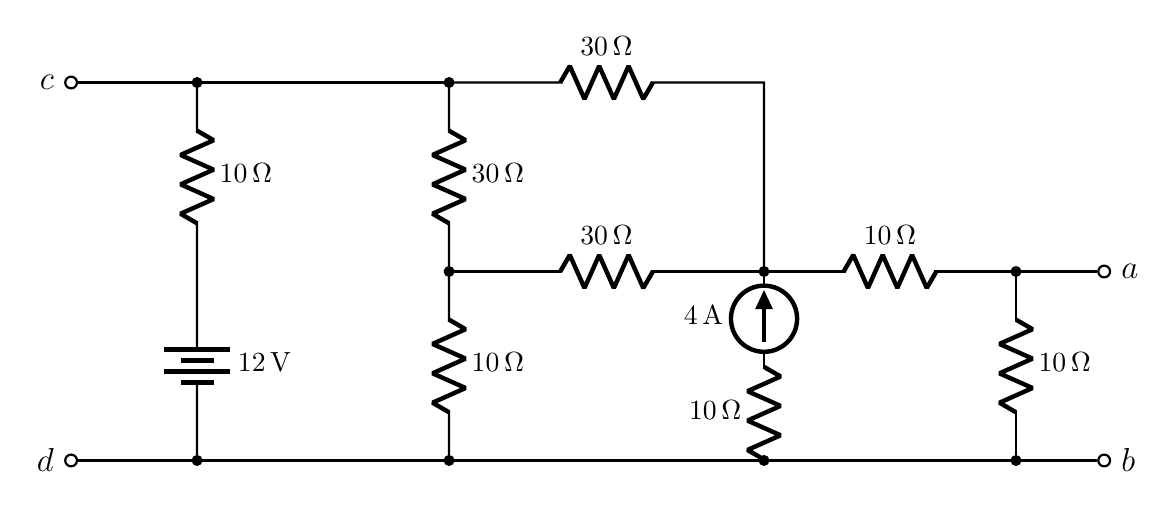
\begin{tikzpicture}[thick , x=1.6cm, y=1.6cm, >=stealth]

    % --- Left Terminals c and d (Using pure TikZ circles to prevent any package errors) ---
    \node[circle, draw, fill=white, inner sep=1.5pt, label=left:{\large $c$}] (C) at (0,3) {};
    \node[circle, draw, fill=white, inner sep=1.5pt, label=left:{\large $d$}] (D) at (0,0) {};
    
    \draw (C) -- (0.5,3);
    \draw (D) -- (0.5,0);

    % --- Main Bottom Rail ---
    \draw (0.5,0) -- (7.5,0);

    % --- First Vertical Branch (10 \Omega Resistor + 12V DC Source) ---
    % Drawing top-to-bottom automatically places the positive (long) plate on top
    \draw (1,3) to[R, l=$10\,\Omega$] (1,1.5)
                to[battery, l=$12\,\text{V}$] (1,0);
    \draw (0.5,3) -- (1,3);

    % --- Connection from Branch 1 to Branch 2 ---
    \draw (1,3) -- (3,3);

    % --- Second Vertical Branch (30 \Omega + 10 \Omega Bridge) ---
    \draw (3,3) to[R, l=$30\,\Omega$] (3,1.5)
                to[R, l=$10\,\Omega$] (3,0);

    % --- Top Horizontal Path (30 \Omega) ---
    \draw (3,3) to[R, l=$30\,\Omega$] (5.5,3) -- (5.5,1.5);

    % --- Middle Horizontal Path (30 \Omega) ---
    \draw (3,1.5) to[R, l=$30\,\Omega$] (5.5,1.5);

    % --- Current Source Branch (4A Source + 10 \Omega Resistor) ---
    % Drawn bottom-to-top so the independent current source arrow points UP
    \draw (5.5,0) to[R, l=$10\,\Omega$] (5.5,0.75)
                  to[I, l=$4\,\text{A}$] (5.5,1.5);

    % --- Rightward Path (10 \Omega) ---
    \draw (5.5,1.5) to[R, l=$10\,\Omega$] (7.5,1.5);

    % --- Rightmost Vertical Branch (10 \Omega) ---
    \draw (7.5,1.5) to[R, l=$10\,\Omega$] (7.5,0);

    % --- Right Terminals a and b ---
    \node[circle, draw, fill=white, inner sep=1.5pt, label=right:{\large $a$}] (A) at (8.2,1.5) {};
    \node[circle, draw, fill=white, inner sep=1.5pt, label=right:{\large $b$}] (B) at (8.2,0) {};
    
    \draw (7.5,1.5) -- (A);
    \draw (7.5,0) -- (B);

    % --- Explicit Connection Junction Dots ---
    \fill (1,3) circle (2pt);
    \fill (1,0) circle (2pt);
    \fill (3,3) circle (2pt);
    \fill (3,1.5) circle (2pt);
    \fill (3,0) circle (2pt);
    \fill (5.5,1.5) circle (2pt);
    \fill (5.5,0) circle (2pt);
    \fill (7.5,1.5) circle (2pt);
    \fill (7.5,0) circle (2pt);


\end{tikzpicture}

\end{center}
\mk{17} \yr{EEE 163 | L-1/T-1 | 2005--06}

\end{enumerate}

%%──────────────────────────────────────────────────────────────────────
\subtopic{cA}{Circuit Analysis (KVL / KCL)}
\label{sub:s1-circuit}

\begin{enumerate}

\item For the circuit shown below, the variable DC voltage source ($V_{dc}$) is adjusted so that the current through the 10\,$\Omega$ resistor is zero. Find the value of $V_{dc}$ and the total power dissipated in the circuit.
\begin{center}
  \begin{circuitikz}[thick, american, scale=1.2, transform shape]

    % Left branch: 23V Voltage Source
    \draw (0,3) to[V, l_=$23\text{ V}$] (0,0);

    % Top-most branch: 30 Ohm Resistor
    \draw (0,3) -- (0,5) to[R, l=$30\ \Omega$] (8,5) -- (8,3);

    % Middle horizontal branches: 5 Ohm and 15 Ohm Resistors
    % The *-* and -* modifiers automatically add the junction dots shown in the image
    \draw (0,3) to[R, l=$5\ \Omega$, *-*] (4,3);
    \draw (4,3) to[R, l=$15\ \Omega$, -*] (8,3);

    % Middle vertical branch: 10 Ohm Resistor and 46V Voltage Source
    \draw (4,3) to[R, l=$10\ \Omega$] (4,1.5);
    \draw (4,1.5) to[V, l=$46\text{ V}$] (4,0);

    % Bottom horizontal branches: 20 Ohm and 25 Ohm Resistors
    \draw (0,0) to[R, l_=$20\ \Omega$, -*] (4,0);
    \draw (4,0) to[R, l_=$25\ \Omega$] (8,0);

    % Right branch: Variable Voltage Source (V_dc)
    \draw (8,3) to[V, l=$V_{\text{dc}}$] (8,0);
    % Drawing the diagonal arrow over the source to indicate it is variable
    \draw[-latex] (7.3, 0.8) -- (8.7, 2.2);

\end{circuitikz}
\end{center}
\mk{20} \yr{EEE 163 | L-1/T-1 | 2024--25}

  
  \item For the circuit shown below, the variable DC voltage source ($V_{dc}$) is adjusted so that the current through the 20\,$\Omega$ resistor is zero. Find the value of $V_{dc}$ and the total power dissipated in the circuit.
\begin{center}
  \begin{circuitikz}[thick, american, scale=1.2, transform shape]

    % Left branch: 23V Voltage Source
    \draw (0,3) to[V, l_=$23\text{ V}$] (0,0);

    % Top-most branch: 30 Ohm Resistor
    \draw (0,3) -- (0,5) to[R, l=$30\ \Omega$] (8,5) -- (8,3);

    % Middle horizontal branches: 5 Ohm and 15 Ohm Resistors
    % The *-* and -* modifiers automatically add the junction dots shown in the image
    \draw (0,3) to[R, l=$5\ \Omega$, *-*] (4,3);
    \draw (4,3) to[R, l=$15\ \Omega$, -*] (8,3);

    % Middle vertical branch: 10 Ohm Resistor and 46V Voltage Source
    \draw (4,3) to[R, l=$10\ \Omega$] (4,1.5);
    \draw (4,1.5) to[V, l=$46\text{ V}$] (4,0);

    % Bottom horizontal branches: 20 Ohm and 25 Ohm Resistors
    \draw (0,0) to[R, l_=$20\ \Omega$, -*] (4,0);
    \draw (4,0) to[R, l_=$25\ \Omega$] (8,0);

    % Right branch: Variable Voltage Source (V_dc)
    \draw (8,3) to[V, l=$V_{\text{dc}}$] (8,0);
    % Drawing the diagonal arrow over the source to indicate it is variable
    \draw[-latex] (7.3, 0.8) -- (8.7, 2.2);

    % Current label i_o with an arrow above the wire
    \draw[-latex] (0.5, 0.4) -- (1.5, 0.4) node[midway, above] {$i_o$};

\end{circuitikz}
\end{center}
\mk{18} \yr{EEE 163 | L-1/T-1 | 2023--24, 2017--18}

\item For the circuit shown below, use an appropriate analysis technique to find the magnitude and the nature of the power associated with the independent current source. 

\begin{center}
  
\begin{circuitikz}[thick ,american, scale=1.2, transform shape]

    % Left branch: 100V Voltage Source
    \draw (0,6) to[V, l=$100\text{ V}$] (0,0);

    % Top horizontal branch (left part): 50 Ohm Resistor
    \draw (0,6) to[R, l=$50\ \Omega$] (4,6);

    % Middle vertical branch 1: 10 Ohm Resistor
    % l_ places the label on the left side of the vertical wire
    \draw (4,6) to[R, l_=$10\ \Omega$] (4,3);
    
    % Manually drawing the i_o current arrow to match the exact position in the image
    \draw[-latex] (3.3, 5.5) -- (3.3, 4.5) node[midway, left] {$i_o$};

    % Top horizontal branch (right part): 10 Ohm Resistor with v_o voltage label
    % v_ places the voltage polarity and label below the resistor
    \draw (4,6) to[R, l=$10\ \Omega$, v_=$v_o$] (8,6);

    % Middle vertical branch 2: Dependent Voltage Source
    \draw (8,6) to[cV, l=$4i_o$] (8,3);

    % Far right vertical branch: 40 Ohm Resistor
    \draw (8,6) -- (11,6) to[R, l=$40\ \Omega$] (11,0);

    % Middle horizontal connecting wire
    \draw (4,3) -- (8,3);

    % Bottom vertical branch 1: Dependent Current Source
    % Drawn top-to-bottom so the arrow points down
    \draw (4,3) to[cI, l_=$0.2v_o$] (4,0);

    % Bottom vertical branch 2: Independent Current Source
    % Drawn bottom-to-top so the arrow points up
    \draw (8,0) to[I, l_=$2\text{ A}$] (8,3);

    % Bottom return wire connecting all branches
    \draw (0,0) -- (11,0);

\end{circuitikz}
\end{center}
\mk{15} \yr{EEE 163 | L-1/T-1 | 2023--24}

\item Would you use the node-voltage method or the mesh-current method to find the power associated with the independent voltage source in the circuit of Figure? Use your selected method to find that power.
\begin{center}
  
\begin{circuitikz}[thick, american, scale=1.2, transform shape]

    % Vertical branches with resistors
    % l=... places the resistance value on the right, v_=... places the voltage on the left
    \draw (0,3) to[R, l=$100\ \Omega$, *-*] (0,0);
    \draw (3,3) to[R, l=$250\ \Omega$, v_=$v_m$, *-*] (3,0);
    \draw (6,3) to[R, l=$500\ \Omega$, v_=$v_\Delta$, *-*] (6,0);
    \draw (9,3) to[R, l=$200\ \Omega$, *-*] (9,0);

    % Bottom return wire
    \draw (0,0) -- (9,0);

    % Middle horizontal branches
    % 20V Independent Voltage Source: 'invert' makes - on left, + on right
    \draw (0,3) to[V, invert, l=$20\text{ V}$] (3,3);
    
    % 200mA Independent Current Source: drawn right-to-left so arrow points left
    \draw (6,3) to[I, l_=$200\text{ mA}$] (3,3);
    
    % 0.4 v_m Dependent Voltage Source: 'invert' makes - on left, + on right
    \draw (6,3) to[cV, invert, l=$0.4\ v_m$] (9,3);

    % Top branch: Dependent Current Source (arrow points right)
    \draw (0,3) -- (0,5) to[cI, l=$0.003\ v_\Delta$] (9,5) -- (9,3);

\end{circuitikz}
\end{center}
\mk{20} \yr{EEE 163 | L-1/T-1 | 2023--24}

\item Determine the maximum power delivered to the variable resistor $R$ shown in the circuit below. Also, determine the percentage change in the delivered maximum power if the 4\,V source is replaced by a 5\,V source.
\begin{center}
  
\begin{circuitikz}[thick , american, scale=1.2, transform shape]

    % ==========================================
    % 1. Coordinate Definitions
    % ==========================================
    \coordinate (BL) at (0,0);      % Bottom Left
    \coordinate (TL) at (0,3);      % Top Left
    \coordinate (TM) at (3,3);      % Top Middle
    \coordinate (BM) at (3,0);      % Bottom Middle
    \coordinate (TR) at (6,3);      % Top Right
    \coordinate (BR) at (6,0);      % Bottom Right

    % ==========================================
    % 2. Left Loop
    % ==========================================
    % 4V Voltage source and top-left 5 Ohm resistor
    \draw (TL) to[V, l=$4\text{ V}$] (BL);
    \draw (TL) to[R, l=$5\ \Omega$] (TM);
               
    % Middle 15 Ohm resistor and return path
    \draw (TM) to[R, l=$15\ \Omega$] (BM)
               -- (BL);

    % ==========================================
    % 3. Right Loop
    % ==========================================
    % Top-right 5 Ohm resistor and vertical resistor R
    \draw (TM) to[R, l=$5\ \Omega$] (TR)
               to[R, l=$R$] (BR);
               
    % Bottom-right 6 Ohm resistor with Voltage Vx
    % 'v_=' places the voltage label below the resistor with correct polarity
    \draw (BM) to[R, l=$6\ \Omega$, v_=$V_x$] (BR);

    % ==========================================
    % 4. Dependent Current Source (Top Branch)
    % ==========================================
    % Placed symmetrically above the right loop
    \draw (TM) -- ++(0,1.5) coordinate (TopL)
               to[cI, l=$3 V_x$] (TopL -| TR)
               -- (TR);

    % ==========================================
    % 5. Junction Nodes (Dots)
    % ==========================================
    % Placing connection dots where 3 or more wires meet
    \node[circ] at (TM) {};
    \node[circ] at (BM) {};
    \node[circ] at (TR) {};

\end{circuitikz}
\end{center}
\mk{20} \yr{EEE 163 | L-1/T-1 | 2022--23}

\item Determine the voltage drop across the 35\,$\Omega$ resistor as shown below.
\begin{center}
  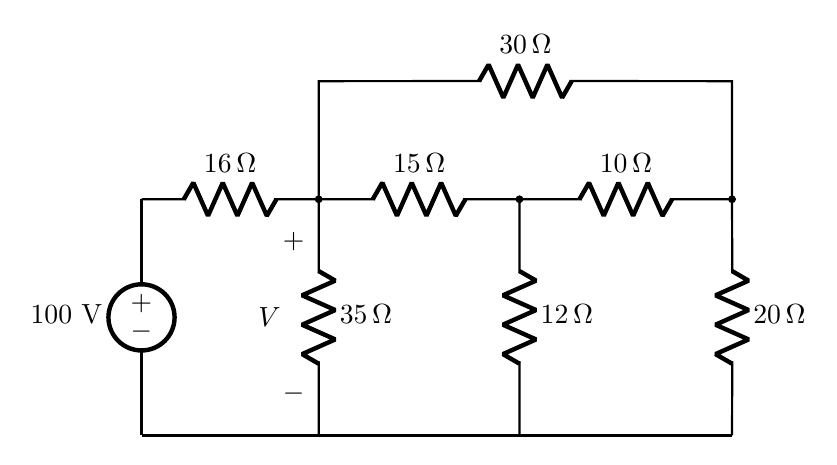
\begin{tikzpicture}[thick, scale=1.5]

    % Bottom wire line
    \draw (0,0) -- (5,0);

    % Leftmost DC Voltage Source branch
    \draw (0,2) to[V, l_=$100\text{ V}$] (0,0);

    % First series resistor from source
    \draw (0,2) to[R, l=$16\,\Omega$] (1.5,2);

    % Main inner junction node
    \draw (1.5,2) node[circle, fill, inner sep=1pt] (nodeA) {};
    
    % Vertical 35 ohm Resistor with voltage drop V
    \draw (1.5,2) to[R, l=$35\,\Omega$, v=$V$] (1.5,0);

    % Top bridging 30 ohm Resistor
    \draw (1.5,2) -- (1.5,3)
                  to[R, l=$30\,\Omega$] (5,3)
                  -- (5,2);

    % Middle row resistors
    \draw (1.5,2) to[R, l=$15\,\Omega$] (3.2,2) node[circle, fill, inner sep=1pt] (nodeB) {}
                  to[R, l=$10\,\Omega$] (5,2) node[circle, fill, inner sep=1pt] (nodeC) {};

    % Vertical 12 ohm Resistor
    \draw (3.2,2) to[R, l=$12\,\Omega$] (3.2,0);

    % Rightmost vertical 20 ohm Resistor
    \draw (5,2) to[R, l=$20\,\Omega$] (5,0);

\end{tikzpicture}

\end{center}
\mk{12} \yr{EEE 163 | L-1/T-1 | 2021--22}

\item For the circuit shown below, find the current $i$ and the power delivered by the 120\,V source.
\begin{center}
  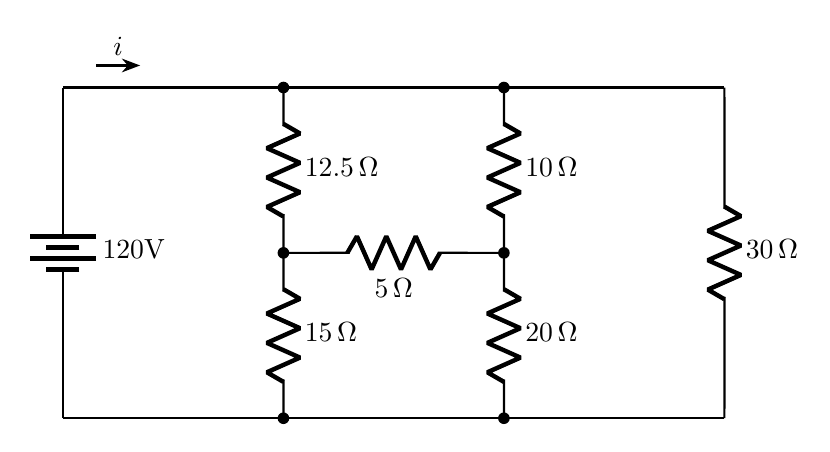
\begin{tikzpicture}[thick, american, scale=1.4]
    
    % Bottom reference rail
    \draw (0,0) -- (6,0);
    
    % Top power rail
    \draw (0,3) -- (6,3);
    
    % Leftmost branch with 120V independent DC voltage source (battery style)
    \draw (0,3) to[battery, l=$120\text{V}$] (0,0);
    
    % Current indicator arrow 'i' at the top left
    \draw[-{Stealth}, thick] (0.3,3.2) -- (0.7,3.2) node[midway, above] {$i$};
    
    % First vertical bridge branch: 12.5 ohm and 15 ohm resistors
    \draw (2,3) to[R, l=$12.5\,\Omega$] (2,1.5)
                to[R, l=$15\,\Omega$] (2,0);
                
    % Second vertical bridge branch: 10 ohm and 20 ohm resistors
    \draw (4,3) to[R, l=$10\,\Omega$] (4,1.5)
                to[R, l=$20\,\Omega$] (4,0);
                
    % Central horizontal bridge resistor (5 ohm) connecting the two vertical branches
    \draw (2,1.5) to[R, l_=$5\,\Omega$] (4,1.5);
    
    % Rightmost parallel branch with 30 ohm resistor
    \draw (6,3) to[R, l=$30\,\Omega$] (6,0);

    % Explicit junction connection dots
    \fill (2,3) circle (1.5pt);
    \fill (2,1.5) circle (1.5pt);
    \fill (2,0) circle (1.5pt);
    \fill (4,3) circle (1.5pt);
    \fill (4,1.5) circle (1.5pt);
    \fill (4,0) circle (1.5pt);

\end{tikzpicture}

\end{center}
\mk{10} \yr{EEE 163 | L-1/T-1 | 2020--21}

\item Find the current delivered by the 10\,V source for the circuit below.
\begin{center}
  \begin{circuitikz}[thick, scale=1.1]
    
    % --- Main Reference Coordinates ---
    % Main bottom wire reference line
    \draw (0,0) to[short] (6,0);
    
    % --- Left Loop (Source & First Stage) ---
    \draw (0,0) to[battery2,invert, l=$10\,\text{V}$] (0,3)
          to[R, l=$2\,\Omega$] (3,3)
          to[R, l=$4\,\Omega$] (3,1.2); % Middle-left vertical node split
          
          
    % Bottom horizontal resistor (left side)
    \draw (0,1.2) to[R, l=$12\,\Omega$] (3,1.2);

    % --- Middle Loop (Second Stage) ---
    \draw (3,3) to[short] (6,3)
          to[R, l=$24\,\Omega$] (6,1.2)
          to[short] (6,0);
          
    % Bottom horizontal resistor (middle side)
    \draw (3,1.2) to[R, l=$12\,\Omega$] (6,1.2);

    % --- Right Loop (Final Branch) ---
    \draw (6,3) to[R, l=$2\,\Omega$] (9,3)
          to[R, l=$6\,\Omega$] (9,1.2)
          to[short] (6,1.2);

    % --- Outer Bridge Wires ---
    % Top bypass shorting rail
    \draw (0,3) -- (0,3.8) -- (6,3.8) -- (6,3);
  

    % --- Connection Node Dots ---
    \node[circle, fill, inner sep=1.2pt] at (3,3) {};
    \node[circle, fill, inner sep=1.2pt] at (3,1.2) {};
    \node[circle, fill, inner sep=1.2pt] at (6,3) {};
    \node[circle, fill, inner sep=1.2pt] at (6,1.2) {};
    \node[circle, fill, inner sep=1.2pt] at (6,0) {};

\end{circuitikz}

\end{center}
\mk{7} \yr{EEE 163 | L-1/T-1 | 2018--19}

\item Find the value of $R$ for the circuit below.
\begin{center}
  \begin{circuitikz}[thick,y=1.5cm , scale=1.1]
    
    % --- Main Outer Loop Wire ---
    \draw (0,0) to[short] (8.5,0);
    
    % --- First Stage: Independent Current Source ---
    \draw (0,0) to[I, l=$8\,\text{A}$] (0,3)
          to[short] (1.5,3);
          
    % --- Second Stage: 4 Ohm Resistor ---
    \draw (1.5,3) to[R, l=$4\,\Omega$] (1.5,0);
    \draw (1.5,3) to[short] (3.5,3);

    % --- Third Stage: Bridge with 3 Ohm, 12 Ohm, and R ---
    \draw (3.5,3) to[R, l=$3\,\Omega$] (3.5,1.8)
          to[short] (2.7,1.8)
          to[R, l=$12\,\Omega$] (2.7,0);
          
    \draw (3.5,1.8) to[short] (4.5,1.8)
          to[R, l=$R$, i^>=$i_x{=}1\,\text{A}$] (4.5,0);
          
    % Connecting top main rail past the bridge
    \draw (3.5,3) to[short] (6.5,3);

    % --- Fourth Stage: 12 Ohm Resistor ---
    \draw (6.5,3) to[R, l=$12\,\Omega$] (6.5,0);
    \draw (6.5,3) to[short] (8.5,3);

    % --- Fifth Stage: Dependent Current Source ---
    \draw (8.5,3) to[cI, l=$4i_x$] (8.5,0); % Closing back to the start

    % --- Connection Node Dots ---
    \node[circle, fill, inner sep=1.2pt] at (1.5,3) {};
    \node[circle, fill, inner sep=1.2pt] at (1.5,0) {};
    \node[circle, fill, inner sep=1.2pt] at (3.5,3) {};
    \node[circle, fill, inner sep=1.2pt] at (3.5,1.8) {};
    \node[circle, fill, inner sep=1.2pt] at (6.5,3) {};
    \node[circle, fill, inner sep=1.2pt] at (6.5,0) {};

\end{circuitikz}

\end{center}
\mk{18} \yr{EEE 163 | L-1/T-1 | 2018--19}

\item Find the power delivered to $R_1$ resistor in the circuit below.
\begin{center}
  \begin{circuitikz}[scale=1.1, thick ]

    % --- Left Source & Initial Resistors ---
    \draw (0,0) to[V,invert,  l=$10\,\text{V}$] (0,3)
          to[R, l=$2\,\Omega$] (2.5,3);
          
    \draw (0,0) to[R, l_=$2\,\Omega$] (2.5,0);

    % --- Upper Bridge (Diamond Structure) ---
    % Split points from coordinate (2.5,3) to (5.5,3)
    \draw (2.5,3) to[short] (2.7,3)
          to[R, l=$10\,\Omega$] (4.1,4)
          to[R, l=$30\,\Omega$] (5.3,3)
          to[short] (5.5,3);
          
    \draw (2.7,3) to[R, l_=$10\,\Omega$] (4.1,2)
          to[R, l_=$30\,\Omega$] (5.3,3);
          
    % Central vertical wire in the upper bridge
    \draw (4.1,4) to[short] (4.1,2);

    % --- Lower Bridge (Diamond Structure) ---
    % Split points from coordinate (2.5,0) to (5.5,0)
    \draw (2.5,0) to[short] (2.7,0)
          to[R, l=$1\,\Omega$] (4,1)
          to[R, l=$2\,\Omega$] (5.3,0)
          to[short] (5.5,0);
          \draw  (2.7, 0)-- (5.3,0);
          
    \draw (2.7,0) to[R, l_=$1\,\Omega$] (4,-1)
          to[R, l_=$2\,\Omega$] (5.3,0);

    % --- Right Side Branch Elements ---
    % Top right branch continuing past bridge
    \draw (5.5,3) to[R, l=$3\,\Omega$] (8,3);
    
    % Rightmost load branch
    \draw (8,3) to[R, l=$R_1{=}1\,\Omega$] (8,0);
    
    % Bottom right branch containing the 3V source
    \draw (8,0) to[short] (7,0)
          to[V, l_=$3\,\text{V}$] (5.5,0);

    % --- Connection Node Dots ---
    \node[circle, fill, inner sep=1.2pt] at (2.7,3) {};
    \node[circle, fill, inner sep=1.2pt] at (5.3,3) {};
    \node[circle, fill, inner sep=1.2pt] at (4.1,4) {};
    \node[circle, fill, inner sep=1.2pt] at (4.1,2) {};
    
    \node[circle, fill, inner sep=1.2pt] at (2.7,0) {};
    \node[circle, fill, inner sep=1.2pt] at (5.3,0) {};

\end{circuitikz}

\end{center}
\mk{5} \yr{EEE 163 | L-1/T-1 | 2018--19}

\item Find $V_1$ of the circuit shown below. Explain why voltage division cannot be used to determine $V_1$.
\begin{center}
    \begin{circuitikz}[scale=1.3, transform shape, thick]

    % Define y-levels for precise alignment
    \def\ytop{3.5}
    \def\ymid{1.75}
    \def\ygnd{0}
    \def\ybot{-1.5}

    % Far left branch: Ground and 20V independent voltage source (+ on top)
    \draw (2, \ybot) --( 0,\ybot) to[V, l=$10\mathrm{V}$, invert] (0,\ytop);

    % Top left wire connecting to the middle-left branch
    \draw (0,\ytop) -- (2,\ytop);

    % Middle-left vertical branch: 10 Ohm and 20 Ohm resistors
    \draw (2,\ytop) to[R, l_=$30k\,\Omega$] (2,\ymid);
    \draw (2,\ymid) to[R, l=$10k\,\Omega$, v=$V_1$, I=$I_1$] (2,\ybot);

    % Middle horizontal cross-branch: Current I_0 and 2V voltage source
    % I_0 arrow points left towards the 10/20 Ohm junction

    % 2V source with + on the left
    \draw (2,\ymid) to[V, l=$1\mathrm{V}$] (5.5,\ymid);

    % Middle-right vertical branch: Dependent current source and 2 Ohm resistor
    % Dependent current source pointing down
    \draw (5.5,\ytop) to[cI, l=$7I_1$] (5.5,\ymid);
    % 2 Ohm resistor connecting to ground
    \draw (5.5,\ymid) to[R, l=$1k\,\Omega$] (5.5,\ybot) ;

    % Top right wire connecting the dependent source to the 10V source
    \draw (5.5,\ytop) -- (8,\ytop);

    % Far right branch: 10V independent voltage source (+ on top)
    \draw (8,\ytop) to[V, l=$30\mathrm{V}$] (8,\ybot);

    % Bottom return wire connecting the 20 Ohm resistor and the 10V source
    \draw (2,\ybot) -- (8,\ybot);
    \draw (5,\ybot) node[ground]{};

    % Add connection dots at the main junctions
    \draw (2,\ymid) node[circ]{};
    \draw (5.5,\ymid) node[circ]{};

\end{circuitikz}

\end{center}
\mk{15} \yr{EEE 163 | L-1/T-1 | 2018--19}

\item The variable resistor ($R_o$) in the circuit shown below is adjusted until the power dissipated in $R_o$ is 250\,W. Find the values of $R_o$ which satisfy this condition.
\begin{center}
  \begin{circuitikz}[thick, y=1.5cm, scale=1.1, every node/.style={transform shape}]

    % --- Main Ground Reference Bottom Rail ---
    \draw (0,0) to[short] (7.5,0);

    % --- Leftmost Branch: 200V Independent Voltage Source ---
    \draw (0,0) to[V, invert, l=$200\,\text{V}$] (0,2.5)
          to[R, l=$50\,\Omega$] (2.5,2.5);

    % --- First Parallel Branch: 200 Ohm Shunt Resistor ---
    \draw (2.5,2.5) to[R, l=$200\,\Omega$] (2.5,0);

    % --- Top Center Branch: 10 Ohm Series Resistor with Current Tracker Ix ---
    \draw (2.5,2.5) to[R, l=$10\,\Omega$, i^=$I_x$] (5.5,2.5);

    % --- Second Parallel Branch: 30 Ohm Resistor + Dependent Voltage Source ---
    \draw (5.5,2.5) to[R, l=$30\,\Omega$] (5.5,1.2)
                    to[cV, l=$20I_x$] (5.5,0);

    % --- Rightmost Branch: Variable Load Resistor Ro ---
    \draw (5.5,2.5) to[short] (7.5,2.5)
                    to[vR, l=$R_o$] (7.5,0);

    % --- Connection Node Dots ---
    \node[circle, fill, inner sep=1.2pt] at (2.5,2.5) {};
    \node[circle, fill, inner sep=1.2pt] at (2.5,0) {};
    \node[circle, fill, inner sep=1.2pt] at (5.5,2.5) {};
    \node[circle, fill, inner sep=1.2pt] at (5.5,0) {};

\end{circuitikz}

\end{center}
\mk{15} \yr{EEE 163 | L-1/T-1 | 2018--19}

\item Find the values of $R_1$ and $R_2$ in the following circuit if the voltmeter and ammeter read 6\,V and 0.6\,A, respectively.
\begin{center}
  \begin{circuitikz}[thick, scale=1.1]

    % --- Main Ground Bottom Rail ---
    \draw (0,0) to[short] (7.5,0);

    % --- Leftmost Branch: 10V Battery & Series 4 Ohm Resistor ---
    \draw (0,0) to[battery2,invert,  l=$10\,\text{V}$] (0,2.5)
          to[R, l=$4\,\Omega$, -*] (2.5,2.5) coordinate (TopLeftJunc);

    % --- Voltmeter Connection Branch ---
    % Connecting down from the post-4-ohm junction to the bottom rail
    \draw (TopLeftJunc) to[rmeter, t=V, v_=$ $] (2.5,0); 

    % --- Parallel Core Stage ---
    % Upper Parallel Branch: Resistor R1
    \draw (TopLeftJunc) -- (2.5,3.3)
          to[R, l=$R_1$] (6.5,3.3) -- (6.5,2.5) coordinate (TopRightJunc);

    % Lower Parallel Branch: 20 Ohm Resistor + Ammeter A in Series
    \draw (TopLeftJunc) to[R, l_=$20\,\Omega$] (4.5,2.5)
          to[rmeter, t=A] (6.5,2.5);

    % --- Rightmost Load Branch: Resistor R2 ---
    \draw (TopRightJunc) to[short] (7.5,2.5) to[R, l=$R_2$] (7.5,0);

\end{circuitikz}

\end{center}
\mk{15} \yr{EEE 163 | L-1/T-1 | 2018--19}

\item Find the voltage $V_{ab}$ for the circuit below.
\begin{center}
  \begin{circuitikz}[thick , scale=1.2]
    % --- Left Side: Voltage Source & First Resistor ---
    \draw (0,0) to[V, invert, l=$10\text{V}$] (0,3)
          to[R, l=$10\,\Omega$] (2,3);
          
    % --- First Two Vertical Parallel Resistors ---
    \draw (2,3) to[R, l=$5\,\Omega$] (2,0);
    \draw (2,3) -- (3.5,3)
          to[R, l=$10\,\Omega$] (3.5,0);
          
    % --- Upper Diagonal Wire Connection ---
    \draw (3.5,3) -- (5,1.5);
    
    % --- Bridge Sub-Network (The 15-Ohm Box & 5-Ohm Resistor) ---
    \draw (3.5,3) -- (6.5,3)
          to[R, l=$5\,\Omega$] (6.5,1.5);
          
    % Box Resistors
    \draw (5,1.5) to[R, l_=$15\,\Omega$] (5,0);
    \draw (6.5,1.5) to[R, l=$15\,\Omega$] (6.5,0);
    
    % Box Internal Connections
    \draw (5,1.5) -- (6.5,1.5); % Top wire of the box
    \draw (5,0) -- (6.5,1.5);   % Diagonal wire inside the box
    
    % --- Bottom Rail Ground/Return Path ---
    \draw (0,0) -- (2,0) -- (3.5,0) -- (5,0) -- (6.5,0);
    
    % --- Right Side: Current Source & Terminals ---
    \draw (6.5,3) -- (8.5,3)
          to[I, l=$5\text{A}$] (8.5,0);
    \draw (6.5,0) -- (8.5,0);
    
    % Terminals a and b
    \draw (8.5,3) to[short, -o] (9.5,3) node[above left] {a};
    \draw (8.5,0) to[short, -o] (9.5,0) node[below left] {b};
    
    % Voltage V_ab Markings
    \node at (9.5, 2.7) {$+$};
    \node at (9.5, 0.3) {$-$};
    \node at (10.0, 1.5) {$V_{ab}$};
    
\end{circuitikz}

\end{center}
\mk{7} \yr{EEE 163 | L-1/T-1 | 2017--18}

\item Consider the circuit below. An ammeter with internal resistance $R_i$ is inserted between a and b to measure $I_o$. Determine the reading of the ammeter if: (i)~$R_i = 0\,\Omega$; (ii)~$R_i = 500\,\Omega$.
\begin{center}
  \begin{circuitikz}[thick, scale=1.2]
    % --- Left Loop ---
    % Vertical 30 kOhm resistor on the far left
    \draw (0,0) to[R, l=$30\,\text{k}\Omega$] (0,3)
          -- (2,3);
          
    % 4 mA Current Source in parallel
    \draw (2,0) to[I, l=$4\,\text{mA}$, *-*] (2,3) node[above] {a};
    
    % Bottom wire connecting left loop paths
    \draw (0,0) -- (2,0);

    % --- Middle Section ---
    % Top resistor with current loop indicator arrow
    \draw (2,3) to[R, l=$2\,\text{k}\Omega$, i_=$I_o$] (5,3) node[above] {b};
    
    % Bottom resistor between loops
    \draw (2,0) to[R, l=$10\,\text{k}\Omega$] (5,0);
    
    % Vertical 20 kOhm resistor acting as a bridge
    \draw (5,3) to[R, l=$20\,\text{k}\Omega$, *-*] (5,0);

    % --- Right Loop ---
    % Top 5 kOhm resistor
    \draw (5,3) to[R, l=$5\,\text{k}\Omega$] (8,3);
    
    % 60V DC Voltage Source on the far right
    \draw (8,3) to[V, l=$60\,\text{V}$] (8,0);
    
    % Bottom return wire completing the circuit
    \draw (5,0) -- (8,0);

\end{circuitikz}

\end{center}
\mk{17} \yr{EEE 163 | L-1/T-1 | 2017--18}

\item For the circuit below: (i)~Find the gain $v_o/v_s$; (ii)~If $V_s = 1$\,V, find $V_{ab}$.
\begin{center}
  \begin{circuitikz}[scale=1.3, thick]
    % --- Left Sub-Circuit ---
    % Node 'a' and the independent voltage source v_s
    \draw (0,0) node[left, font=\bfseries] {a} node[circle, fill, inner sep=1.5pt]{}
          to[V,invert, l=$v_s$] (0,2.5)
          to[R, l=$200\,\Omega$] (2.5,2.5)
          to[R, l=$100\,\Omega$] (2.5,0)
          -- (0,0);

    % 2k Ohm resistor and dependent voltage source (v_o / 1000)
    % 'invert' ensures the '+' terminal stays on top when drawing downwards
    \draw (2.5,2.5) to[R, l=$2\text{k}\Omega$] (5,2.5)
      to[cV, l=$\frac{v_o}{1000}$, i>=$I_o$] (5,0)
      -- (2.5,0);

    % --- Bottom Connecting Link ---
    % 5V independent source and 10k Ohm resistor linking the two stages
    \draw (5,0) to[V, invert,l_=$5\text{V}$] (6.5,0)
          to[R, l_=$10\text{k}\Omega$] (9,0);

    % --- Right Sub-Circuit ---
    % Dependent current source 40I_o
    \draw (9,2.5) to[cI, l=$40I_o$] (9,0);
    
    % Node 'b' and the 10k Ohm resistor with voltage output v_o
    \draw (9,2.5) -- (11.5,2.5) node[above, font=\bfseries] {b} node[circle, fill, inner sep=1.5pt]{}
          to[R, l=$10\text{k}\Omega$, v=$v_o$] (11.5,0)
          -- (9,0);
          
\end{circuitikz}

\end{center}
\mk{15+3} \yr{EEE 163 | L-1/T-1 | 2015--16}

\item For the circuit shown below, calculate the power supplied by each voltage source and current source. Also verify the fact that the summation of total power supplied by each element of the circuit is zero.
\begin{center}
  \begin{circuitikz}[scale=1.3, transform shape, thick]

    % Left branch: 10V independent voltage source
    \draw (0,3) to[V, l=$10\mathrm{V}$] (0,0);

    % Top-left branch: 20 ohm resistor and 5V independent voltage source (+ on left)
    \draw (0,3) to[R, l=$20\,\Omega$] (2.5,3)
                to[V, l=$5\mathrm{V}$] (5,3);

    % Bottom-left branch: 10 ohm resistor
    \draw (0,0) to[R, l_=$10\,\Omega$] (5,0);

    % Middle branch: 3A current source pointing up and 3 ohm resistor
    \draw (5,0) to[I, l_=$3\mathrm{A}$] (5,1.5)
                to[R, l_=$3\,\Omega$] (5,3);

    % Ground node at the intersection of the bottom branches
    \draw (5,0) node[ground]{};

    % Top-right branch: 5A current source pointing right
    \draw (5,3) to[I, l=$5\mathrm{A}$] (9,3);

    % Rightmost branch: 8 ohm resistor
    \draw (9,3) to[R, l=$8\,\Omega$] (9,0);

    % Bottom-right branch: 4 ohm resistor
    \draw (9,0) to[R, l=$4\,\Omega$] (5,0);


\end{circuitikz}

\end{center}
\mk{17} \yr{EEE 163 | L-1/T-1 | 2014--15}

\item Draw the waveshapes of current for the given waveshapes of charge as shown below.
\begin{center}
  \begin{tikzpicture}[scale=1.5]

    % --- LEFT: Square Wave ---
    \begin{scope}[shift={(0,0)}]
        % Axes
        \draw[->, thick] (0,-1.5) -- (0,1.5) node[above] {$v$};
        \draw[->, thick] (-0.2,0) -- (2.5,0) node[right] {$t$};
        
        % Waveform
        \draw[thick] (0,1) -- (1,1) -- (1,-1) -- (2,-1) -- (2,1) -- (2.4,1);
    \end{scope}

    % --- MIDDLE: Triangular Wave ---
    \begin{scope}[shift={(3.5,0)}]
        % Axes
        \draw[->, thick] (0,-1.5) -- (0,1.5) node[above] {$q$};
        \draw[->, thick] (-0.2,0) -- (2.5,0) node[right] {$t$};
        
        % Waveform
        \draw[thick] (0,0) -- (0.8,1) -- (1.8,-1) -- (2.4,0.2);
    \end{scope}

    % --- RIGHT: Sine Wave ---
    \begin{scope}[shift={(7,0)}]
        % Axes
        \draw[->, thick] (0,-1.5) -- (0,1.5) node[above] {$q$};
        \draw[->, thick] (-0.2,0) -- (2.8,0) node[right] {$t$};
        
        % Waveform (One full cycle over x=0 to x=2.4)
        \draw[thick, domain=0:2.4, samples=100] plot (\x, {sin(\x * 150)}); 
    \end{scope}

\end{tikzpicture}

\end{center}
\mk{9} \yr{EEE 163 | L-1/T-1 | 2013--14}

\item Write the conditions for linearity. Can you apply the maximum power transfer theorem for a linear circuit? Explain.
\mk{7} \yr{EEE 163 | L-1/T-1 | 2013--14}

\item Define active and passive circuit elements with examples. Classify active elements and specify each of them.
\mk{10} \yr{EEE 163 | L-1/T-1 | 2012--13}

\item How do the practical voltage and current sources differ from ideal voltage and current sources?
\mk{10} \yr{EEE 163 | L-1/T-1 | 2011--12}

\item Write down the statements of Kirchhoff's voltage and current laws.
\mk{5} \yr{EEE 163 | L-1/T-1 | 2011--12}

\item Calculate all the branch currents $I_1$ to $I_5$ in the circuit shown below.
\begin{center}
  \begin{circuitikz}[thick,american]
    % --- Outer Loop Components ---
    % Left DC Voltage Source
    \draw (0,0) to[battery1,invert, l=10~V] (0,4)
    % Top branch resistors and nodes
          to[R, l=5~$\Omega$] (2.5,4) node[circle, fill, inner sep=1.5pt] (N1) {}
          to[R, l=10~$\Omega$] (5.5,4) node[circle, fill, inner sep=1.5pt] (N2) {}
          to[R, l=5~$\Omega$] (8.5,4)
    % Right vertical resistor
          -- (8.5,3.5) to[R, l=20~$\Omega$] (8.5,0.5) -- (8.5,0)
    % Bottom branch resistors and nodes
          to[R, l=5~$\Omega$] (5.5,0) node[circle, fill, inner sep=1.5pt] (N4) {}
          to[R, l=10~$\Omega$] (2.5,0) node[circle, fill, inner sep=1.5pt] (N3) {}
          to[R, l=5~$\Omega$] (0,0);

    % --- Central Bridge Network (With Crossover Jump/Arc) ---
    % ১. N1 থেকে N4 পর্যন্ত কোণাকুণি সোজা তার (যা ৫০ ওহম রেজিস্টর ধারণ করে)
\draw (N1) to[R, l=$50\,\Omega$, pos=0.25] ( 3.7,2.4)-- (N4);    
    % ২. N3 থেকে আসা তারটি ৫০ ওহম রেজিস্টর পার হয়ে কোণাকুণি তারের ওপর দিয়ে arc করে চলে যাবে
    \draw (N3) -- (2.5, 1.8) 
          to[R, l=50~$\Omega$] (3.9, 1.8) -- (4.0, 1.8)
          arc[start angle=180, end angle=0, radius=0.15] % এই অংশটি আর্কের (লুপ) কাজ করবে
          -- (5.5, 1.8);
    
    % ৩. N2 থেকে আসা উলম্ব তারটি ডান পাশের জংশনে এসে মিলবে
    \draw (N2) -- (5.5, 1.8);

    % --- Custom Current Arrows & Labels ---
    % Current I1
    \draw[->, >=stealth, thick] (1.0, 3.3) -- (1.7, 3.3) node[midway, below] {$I_1$};
    
    % Current I3
    \draw[->, >=stealth, thick] (3.6, 4.7) -- (4.3, 4.7) node[midway, above] {$I_3$};
    
    % Current I4
    \draw[->, >=stealth, thick] (6.6, 3.3) -- (7.3, 3.3) node[midway, below] {$I_4$};
    
    % Current I2
    \draw[->, >=stealth, thick] (2.5, 3.2) -- (2.9, 2.7) node[pos=0.7, left] {$I_2$};
    
    % Current I5
    \draw[->, >=stealth, thick] (5.8, 3.2) -- (5.8, 2.5) node[midway, right] {$I_5$};

\end{circuitikz}

\end{center}
\mk{20} \yr{EEE 163 | L-1/T-1 | 2011--12}

\item Find the power dissipated in 10\,$\Omega$ ($P_{10}$) and 1\,$\Omega$ ($P_1$) resistors in the circuit below.
\begin{center}
  \begin{circuitikz}[american  , thick]
    % --- Loop 1: 25A Current Source & 4 Ohm Resistor ---
    \draw (0,0) to[I, l={25 A}] (0,3)
          -- (2,3) to[R, l={4 $\Omega$}] (2,0)
          -- (0,0);

    % --- Connection 1: 10 Ohm Resistor with Power Label ---
    \draw (2,3) to[R, l_={10 $\Omega$}, a^={$P_{10} = ?$}] (5,3);
    \draw (2,0) -- (5,0);

    % --- Loop 2: 20A Current Source & 2 Ohm Resistor ---
    \draw (5,0) to[I, l={20 A}] (5,3)
          -- (7,3) to[R, l={2 $\Omega$}] (7,0)
          -- (5,0);

    % --- Connection 2: 1 Ohm Resistor with Power Label ---
    \draw (7,3) to[R, l_={1 $\Omega$}, a^={$P_1 = ?$}] (10,3);
    \draw (7,0) -- (10,0);

    % --- Loop 3: 10 Ohm Parallel Resistor & 20V Source ---
    \draw (10,3) to[R, l={10 $\Omega$}] (10,0);
    \draw (10,3) -- (12,3) 
          to[V, l={20 V}] (12,0)
          -- (10,0);
\end{circuitikz}

\end{center}
\mk{25} \yr{EEE 163 | L-1/T-1 | 2011--12}

\item For the following circuit, find the power delivered to $R_0$ in the circuit below.
\begin{center}
  \begin{circuitikz}[american , thick]
    % --- Left Loop: 3mA Current Source & 4k Ohm Parallel Resistor ---
    \draw (0,0) to[I, l={3 mA}] (0,3)
          -- (2,3) to[R, l={4 k$\Omega$}] (2,0)
          -- (0,0);

    % --- Top Path: 8k Ohm Series Resistor ---
    \draw (2,3) to[R, l={8 k$\Omega$}] (5,3);

    % --- Vertical Branch: 20k Ohm Resistor & 10V DC Source (with + on top) ---
    \draw (5,3) to[R, l={20 k$\Omega$}] (5,1.5)
          to[V, l={10 V}] (5,0);

    % --- Top Path: 2.5k Ohm Series Resistor ---
    \draw (5,3) to[R, l={2.5 k$\Omega$}] (8,3);

    % --- Vertical Branch: 10k Ohm Resistor ---
    \draw (8,3) to[R, l={10 k$\Omega$}] (8,0);

    % --- Top Path: Horizontal 10V Source (with + on left) ---
    \draw (8,3) to[V, l={10 V}] (10.5,3) -- (11,3);

    % --- Rightmost Branch: Ro = 5k Ohm Resistor ---
    \draw (11,3) to[R, l={$R_o = 5$ k$\Omega$}] (11,0);

    % --- Completing the bottom return wire rail ---
    \draw (2,0) -- (11,0);


\end{circuitikz}

\end{center}
\mk{23} \yr{EEE 163 | L-1/T-1 | 2011--12}

\item In the circuit below, the current through the $R_1$ resistor is 1\,A. Find source voltage $V_g$.
\begin{center}
  \begin{circuitikz}[thick, american, x=1.4cm, transform shape]
    
    % --- Main Horizontal Nodes & Paths ---
    % Bottom Rail Left
    \draw (0,0) -- (2,0);
    
    % Leftmost Column: DC Source Vg
    \draw (0,0) to[battery2,invert, l=$V_g$] (0,3);
    
    % Top path: 5 Ohm resistor to Node 1
    \draw (0,3) to[R, l=$5\Omega$] (2,3);
    
    % Vertical 140 Ohm resistor at Node 1
    \draw (2,3) to[R, l=$140\Omega$, *-*] (2,0);
    
    % Bottom path: 4 Ohm resistor to Central Bottom Node
    \draw (2,0) to[R, l=$4\Omega$] (5,0);
    
    % --- Middle Section ---
    % Top path: 12 Ohm resistor from Node 1 to Node 2
    \draw (2,3) to[R, l=$12\Omega$, *-*] (5,3);
    
    % Vertical 16 Ohm resistor from Node 2 to Central Bottom Node
    \draw (5,3) to[R, l=$16\Omega$] (5,0);
    
    % Left Diagonal: 48 Ohm resistor
    \draw (2,3) to[R, l=$48\Omega$, pos=0.4] (5,0);
    
    % --- Right Section ---
    % Top path: 12 Ohm resistor from Node 2 to Node 3
    \draw (5,3) to[R, l=$12\Omega$, -*] (8,3);
    
    % Right Diagonal: 9 Ohm resistor
    \draw (8,3) to[R, l=$9\Omega$, pos=0.4] (5,0);
    
    % Bottom path: 6 Ohm resistor from Central Bottom Node to Bottom Right
    \draw (5,0) to[R, l=$6\Omega$, -*] (8,0);
    
    % Rightmost Vertical Column: Resistor R1 (12 Ohm)
    \draw (8,3) to[R, l=$R_1$, a=$12\Omega$] (8,0);
    
    % 1A Current arrow indicator next to R1
    \draw[->, thick] (9, 1.8) -- (9, 1.2) node[midway, right] {$1\text{A}$};
    
    % --- Top Bypass Wire ---
    % 12 Ohm resistor bypassing the top network from Node 1 to Node 3
    \draw (2,3) -- (2,4.5) to[R, l=$12\Omega$] (8,4.5) -- (8,3);
    
    
\end{circuitikz}
\end{center}
\mk{18} \yr{EEE 163 | L-1/T-1 | 2010--11}

\item Calculate the value of $\alpha$ and $\beta$ for which the linear circuit below has the current and voltage relationship as shown below.

\begin{center}
  \begin{circuitikz}[thick,scale=1.2, transform shape]

    % Top branch with independent V source (- to + from left to right)
    \draw (0,4) to[V, l=$1\,\text{V}$, invert] (4,4);
    
    % i_y current arrow above the left side of the top branch
    \draw[thick, ->] (0.2, 4.6) -- (1.0, 4.6) node[midway, above] {$i_y$};

    % Left vertical branch (Resistor and wire)
    \draw (0,4) to[R, l=$11\,\Omega$] (0,2);
    % Manual v_x polarity and label to match image exactly
    \node at (-0.6, 3.6) {$-$};
    \node at (-0.6, 2.4) {$+$};
    \node at (-0.8, 3.0) {$v_x$};
    % Bottom wire of the left branch
    \draw (0,2) -- (0,0);

    % Middle horizontal branch (Dependent Voltage Source, + on left)
    \draw (0,2) to[cV, l=$\alpha i_y$] (4,2);

    % Right vertical branch (Two Resistors)
    \draw (4,4) to[R, l_=$11\,\Omega$] (4,2); % l_ puts the label on the right side
    \draw (4,2) to[R, l_=$13\,\Omega$] (4,0);

    % Bottom branch (Dependent Current Source pointing left)
    % Drawing from right to left makes the arrow point left. 
    % l_ places the label "above" the left-pointing path.
    \draw (4,0) to[cI, l_=$\beta v_x$] (0,0);

    % Terminals and output
    \draw (4,4) to[short, i=$i$, -o] (6,4) node[above] {$a$};
    \draw (4,0) to[short, -o] (6,0) node[right] {$b$}; 
    
    % v_ab labels and polarity
    \node at (6.5, 4.0) {$+$};
    \node at (6.5, 0.0) {$-$};
    \node at (7.0, 2.0) {$v_{ab}$};

\end{circuitikz}
\begin{tikzpicture}[scale=1.2, >=stealth]

    % --- Axes ---
    % X-axis (v_ab)
    \draw[->, thick] (-0.5, 0) -- (6, 0) node[below right] {$v_{ab}$};
    
    % Y-axis (i_A (amps))
    \draw[->, thick] (0, -2.5) -- (0, 2.5) node[above right] {$i \text{ (amps)}$};

    % --- Ticks and Labels on Y-axis ---
    % 0.2 tick
    \draw[thick] (-0.1, 1.2) -- (0.1, 1.2);
    \node[left] at (-0.1, 1.2) {$0.2$};
    
    % -0.2 tick
    \draw[thick] (-0.1, -1.2) -- (0.1, -1.2);
    \node[left] at (-0.1, -1.2) {$-0.2$};
    
    % -0.327 intercept point
    \node[left] at (-0.1, -2.0) {$-0.327$};

    % --- Ticks and Labels on X-axis ---
    % 20 V tick
    \draw[thick] (2, -0.1) -- (2, 0.1);
    \node[below] at (2, -0.1) {$20\,\text{V}$};
    
    % 40 V tick
    \draw[thick] (4, -0.1) -- (4, 0.1);
    \node[below] at (3.9, -0.1) {$40\,\text{V}$};

    % --- The Plot Line ---
    % Line starting from (0, -0.327 equivalent) through the x-intercept
    \draw[thick] (0, -2.0) -- (5.5, 0.62);

    % --- Annotations ---
    % Arrow pointing to the 40.26 V x-intercept
    \draw[<-, thick] (4.25, 0.05) -- (4.25, 0.8) node[above] {$40.26\,\text{V}$};

\end{tikzpicture}
\end{center}

\mk{20} \yr{EEE 163 | L-1/T-1 | 2008--09}

\item For the circuit shown below, the voltage across the 20\,k$\Omega$ resistor was found to be 1.49\,V when a voltmeter was used to measure it. Calculate the resistance of the voltmeter.
\begin{center}
  \begin{circuitikz}[thick ,scale=1.0]
    \draw (0,0) node[ground]{} -- (8,0);
    
    % Main left and top frame
   \draw (0,0) to[isource, l_=$2\text{ mA}$, invert] (0,3) -- (3,3);
    
    % First middle vertical branch (2.5 kOhm resistor)
    \draw (3,3) to[R, l=$2.5\text{ k}\Omega$, *-] (3,0);
    
    % Main top wire cont., horizontal 10 kOhm resistor, and node markers
  \draw  (3,3) to[R, l=$10\text{ k}\Omega$, *-*] (6,3) -- (8,3);
    
    % Second middle vertical branch (3 mA source and label A)
   \draw (6,0) to[isource, l=$3\text{ mA}$] (6,3);
    
    % Far right loop with 20 kOhm resistor
    \draw (8,3) to[R, l=$20\text{ k}\Omega$] (8,0);
    
    % explicit nodes for precise label placement for v0, matching image style
    \node at (7.7, 2.7) {$+$};
    \node at (7.7, 0.3) {$-$};
    \node at (7.6, 1.5) {$v_0$};
    
    % Dummy connections to finish looped structure if needed,
    % but stage draws handle this. Ground wire is already fully drawn.
    
    % Bypass loop with the Voltage-Controlled Current Source
    \draw (3,3) -- (3,4.5);
    \draw (6,4.5) to[controlled current source, l_=$2 \times 10^{-3} v_0$] (3,4.5);
    \draw (6,4.5) -- (6,3);

\end{circuitikz}
\end{center}
\mk{15} \yr{EEE 163 | L-1/T-1 | 2008--09}

\item For the circuit shown below, determine $R_i$, $R_o$, and $V_0$ when $R_G = 10\,\text{M}\Omega$, $g = 5\,\text{mS}$, $R_D = 1\,\text{k}\Omega$, $R_1 = 10\,\Omega$, $R_2 = 100\,\Omega$, $R_s = 100\,\Omega$.
\begin{center}
  
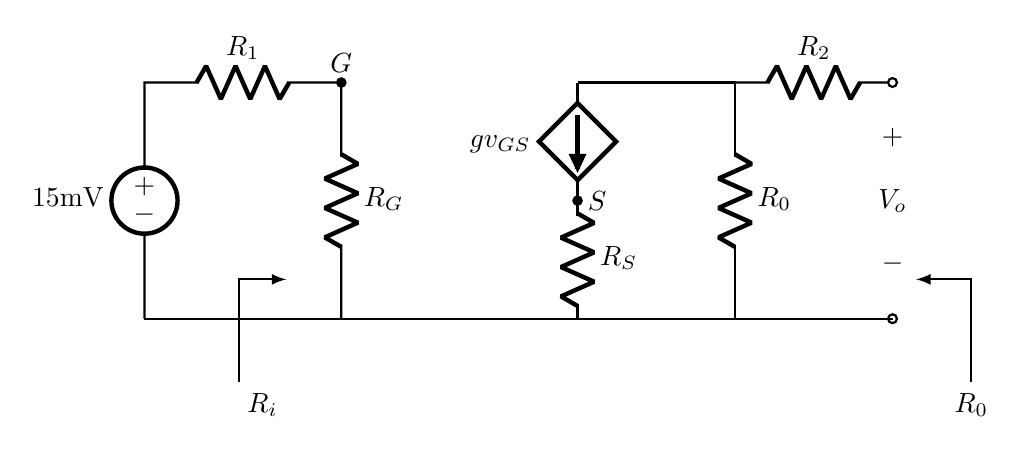
\begin{tikzpicture}[american, thick]

    % --- Input Side ---
    % 15mV Voltage Source and R1
    \draw (0,0) to[V,invert, l=$15\text{mV}$] (0,3)
          to[R, l=$R_1$] (2.5,3) coordinate (G);
    
    % Node G
    \filldraw (G) circle (1.5pt) node[above] {$G$};
    
    % Resistor RG
    \draw (G) to[R, l=$R_G$] (2.5,0);
    
    % --- Dependent Source & Output Side ---
    % Dependent Current Source
    \draw (5.5,3) to[cI, l_=$g v_{GS}$] (5.5,1.5) coordinate (S);
    
    % Node S and Resistor RS
    \filldraw (S) circle (1.5pt) node[right] {$S$};
    \draw (S) to[R, l=$R_S$] (5.5,0);
    
    % Top wire to R0
    \draw (5.5,3) -- (7.5,3) to[R, l=$R_0$] (7.5,0);
    
    % Resistor R2 and Output Terminals
    \draw (7.5,3) to[R, l=$R_2$] (9.5,3) node[ocirc] {};
    \draw (9.5,0) node[ocirc] {};
    
    % Bottom Common Line
    \draw (0,0) -- (9.5,0);
    
    % --- Labels and Indicators ---
    % Output Voltage (Vo) labels
    \node at (9.5, 2.3) {$+$};
    \node at (9.5, 1.5) {$V_o$};
    \node at (9.5, 0.7) {$-$};
    
    % Input Resistance (Ri) Arrow
    \draw[-latex] (1.2, -0.8) -- (1.2, 0.5) -- (1.8, 0.5);
    \node at (1.5, -1.1) {$R_i$};
    
    % Output Resistance (R0) Arrow
    \draw[-latex] (10.5, -0.8) -- (10.5, 0.5) -- (9.8, 0.5);
    \node at (10.5, -1.1) {$R_0$};

\end{tikzpicture}
\end{center}
\mk{15} \yr{EEE 163 | L-1/T-1 | 2007--08}

\item Find the value of $I$, $I_1$, $I_2$, $I_3$ \& $I_4$ for the circuit shown below.
\begin{center}
  \begin{circuitikz}[thick, y=1.2cm]

    % ---------------------------------------------------
    % Coordinate Definitions for Precision
    % ---------------------------------------------------
    % Top row
    \coordinate (T0) at (0,4);
    \coordinate (T2) at (2,4);
    \coordinate (T8) at (8,4);
    \coordinate (T10) at (10,4);
    
    % Middle-Top row 
    \coordinate (M0) at (0,1);
    \coordinate (M2) at (2,2);
    \coordinate (M8) at (8,1);
    
    % Bottom I2 row (Short circuit line)
    \coordinate (B2) at (2,0);
    \coordinate (B8) at (8,0);
    \coordinate (B10) at (10,0);
    
    % Lowest row (Bottom 4k resistor)
    \coordinate (L2) at (2,-2);
    \coordinate (L8) at (8,-2);

    % ---------------------------------------------------
    % Circuit Branches
    % ---------------------------------------------------
    
    % Outer Loop Top (Current I)
    \draw (T0) -- (0,5.5) to[short, i=$I$] (8,5.5) -- (T8);

    % Left 20V Source
    \draw (M0) to[V,invert, l=$20\text{V}$] (T0);

    % Top 2k Resistor (I1 goes left)
    \draw (T2) to[R, l=$2\text{ k}\Omega$, i<=$I_1$] (T8);

    % Inner Left 5mA Source (Vertical)
    \draw (T2) to[I,l=$5\text{ mA}$] (B2);
    \draw (B2) -- (L2);

    % Middle Horizontal line with jump over x=2, and 4k Resistor (I4 goes left)
    \draw (M0) -- (1.8,1) arc[start angle=180, end angle=0, radius=0.2] -- (3,1) 
          to[R, l_=$4\text{ k}\Omega$, i<=$I_4$] (M8);

    % Diagonal Branch (1k + 10V) - (5,3) is the exact midpoint
    \draw (T2) to[R, l_=$1\text{ k}\Omega$, i^=$I_3$] (5,2) to[V,invert,  l^=$10\text{V}$] (M8);

    % Inner Right 3mA Source (Vertical)
    \draw (M8) to[I, l=$3\text{ mA}$] (T8);
    

    % Vertical line from M8 downwards (crossed by I2)
    \draw (M8) -- (L8);

    % Connection to the far right
    \draw (T8) -- (T10);
    \node[circ] at (T10) {};

    % ---------------------------------------------------
    % Rightmost Branches & Short Circuits
    % ---------------------------------------------------
    
    % Rightmost 1k Resistor
    \draw (T10) to[R, l=$1\text{ k}\Omega$] (B10);
    
    % Parallel Short Circuit on the far right
    \draw (T10) -- (11.5,4) -- (11.5,0) -- (B10);
    \node[circ] at (B10) {};

    % I2 Short Line (y=0) with jump over the vertical wire at x=8
    \draw (B2) to[short, i<=$I_2$] (7.8,0) arc[start angle=180, end angle=0, radius=0.2] -- (B10);

    % Bottom-most 4k Resistor
    \draw (L2) to[R, l=$4\text{ k}\Omega$] (L8);



\end{circuitikz}
\end{center}
\mk{20} \yr{EEE 163 | L-1/T-1 | 2006--07}

\item For the circuit shown below, find the currents $I_1$ and $I_2$ using branch current method.
\begin{center}
  
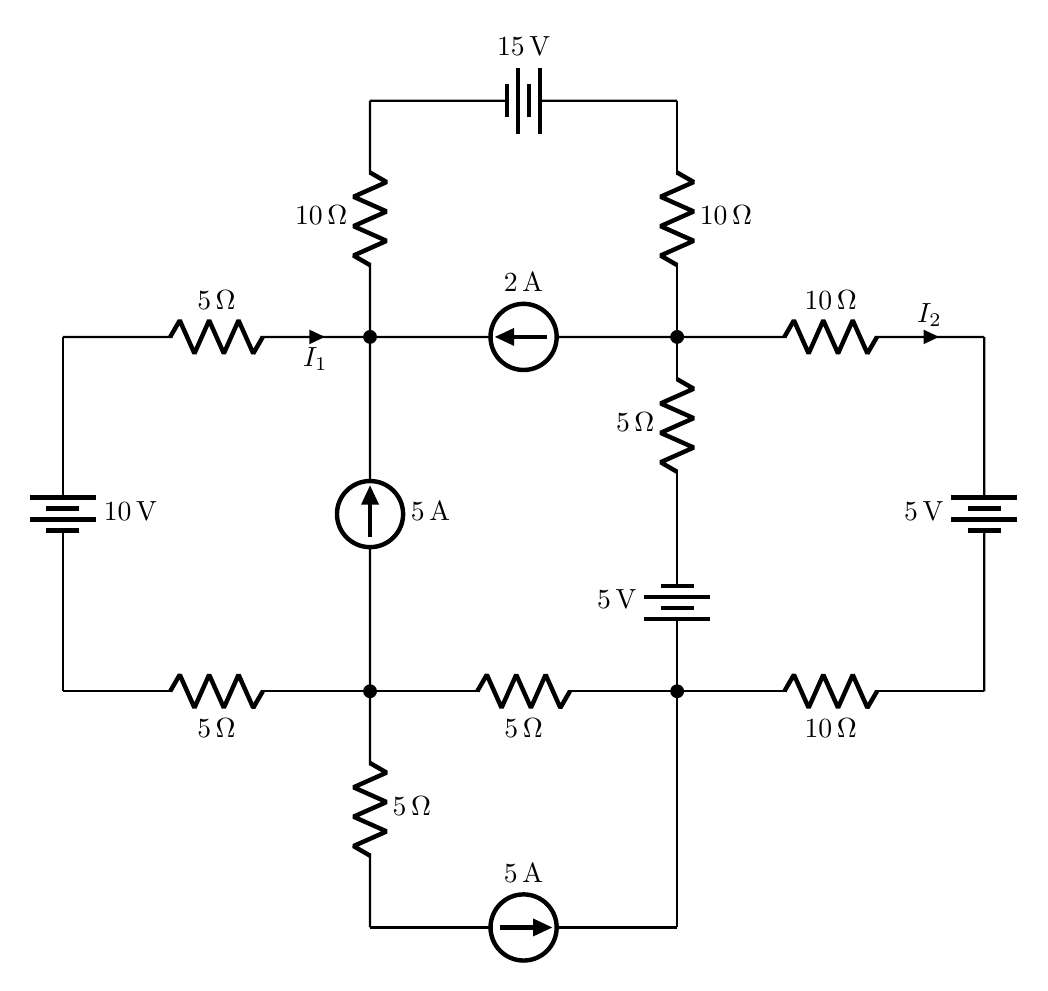
\begin{tikzpicture}[thick,x=1.3cm, y=1.5cm, >=stealth]

    % --- Left Loop ---
    % 10V battery drawn bottom-to-top puts the positive (long) terminal on top
    \draw (0,3) to[battery, l=$10\,\text{V}$] (0,0);
    \draw (0,3) to[R, l=$5\,\Omega$, i_=$I_1$] (3,3); % i_ puts the label I_1 below the arrow
    \draw (0,0) to[R, l_=$5\,\Omega$] (3,0); % l_ puts the label below the resistor

    % --- Middle-Left Vertical Branch ---
    \draw (3,0) to[I, l_=$5\,\text{A}$] (3,3); % Arrow points up

    % --- Top Loop ---
    \draw (3,3) to[R, l=$10\,\Omega$] (3,5);
    % Drawn right-to-left so the positive (long) plate is on the left
    \draw (6,5) to[battery, l_=$15\,\text{V}$] (3,5); 
    \draw (6,5) to[R, l=$10\,\Omega$] (6,3);

    % --- Middle Horizontal Branches ---
    % Drawn right-to-left so the current arrow points left
    \draw (6,3) to[I, l_=$2\,\text{A}$] (3,3); 
    \draw (3,0) to[R, l_=$5\,\Omega$] (6,0);

    % --- Right-Middle Vertical Branch ---
    % Drawn bottom-to-top to put the positive battery terminal on top
    \draw (6,0) to[battery, l=$5\,\text{V}$] (6,1.5) 
                to[R, l=$5\,\Omega$] (6,3);

    % --- Right Loop ---
    \draw (6,3) to[R, l=$10\,\Omega$, i=$I_2$] (9,3); % i puts the label I_2 above the arrow
    \draw (6,0) to[R, l_=$10\,\Omega$] (9,0);
    \draw (9,3) to[battery, l_=$5\,\text{V}$] (9,0); % Drawn bottom-to-top for positive plate on top

    % --- Bottom Loop ---
    \draw (3,0) to[R, l=$5\,\Omega$] (3,-2);
    \draw (3,-2) to[I, l=$5\,\text{A}$] (6,-2); % Arrow points right
    \draw (6,-2) -- (6,0); % Connecting wire back to the grid

    % --- Explicit Junction Dots ---
    \fill (3,3) circle (2.5pt);
    \fill (3,0) circle (2.5pt);
    \fill (6,3) circle (2.5pt);
    \fill (6,0) circle (2.5pt);

\end{tikzpicture}

\end{center}
\mk{18} \yr{EEE 163 | L-1/T-1 | 2005--06}

\end{enumerate}

%%──────────────────────────────────────────────────────────────────────
\subtopic{cA}{Mesh / Loop Analysis}
\label{sub:s1-mesh}

\begin{enumerate}
  
  
  \item For the circuit shown below, use mesh analysis techniques to find the power associated with the 40\,$\Omega$ resistor.

\begin{center}
  
\begin{circuitikz}[thick ,american,  transform shape]

    % Left branch: 100V Voltage Source
    \draw (0,6) to[V, l=$100\text{ V}$] (0,0);

    % Top horizontal branch (left part): 50 Ohm Resistor
    \draw (0,6) to[R, l=$50\ \Omega$] (4,6);

    % Middle vertical branch 1: 10 Ohm Resistor
    % l_ places the label on the left side of the vertical wire
    \draw (4,6) to[R, l_=$10\ \Omega$] (4,3);
    
    % Manually drawing the i_o current arrow to match the exact position in the image
    \draw[-latex] (3.3, 5.5) -- (3.3, 4.5) node[midway, left] {$i_o$};

    % Top horizontal branch (right part): 10 Ohm Resistor with v_o voltage label
    % v_ places the voltage polarity and label below the resistor
    \draw (4,6) to[R, l=$10\ \Omega$, v_=$v_o$] (8,6);

    % Middle vertical branch 2: Dependent Voltage Source
    \draw (8,6) to[cV, l=$4i_o$] (8,3);

    % Far right vertical branch: 40 Ohm Resistor
    \draw (8,6) -- (11,6) to[R, l=$40\ \Omega$] (11,0);

    % Middle horizontal connecting wire
    \draw (4,3) -- (8,3);

    % Bottom vertical branch 1: Dependent Current Source
    % Drawn top-to-bottom so the arrow points down
    \draw (4,3) to[cI, l_=$0.2v_o$] (4,0);

    % Bottom vertical branch 2: Independent Current Source
    % Drawn bottom-to-top so the arrow points up
    \draw (8,0) to[I, l_=$2\text{ A}$] (8,3);

    % Bottom return wire connecting all branches
    \draw (0,0) -- (11,0);

\end{circuitikz}
\end{center}
  \mk{20} \yr{EEE 163 | L-1/T-1 | 2022--23}

\item Find the power supplied by the 30\,V voltage source as shown below using mesh analysis.
\begin{center}
  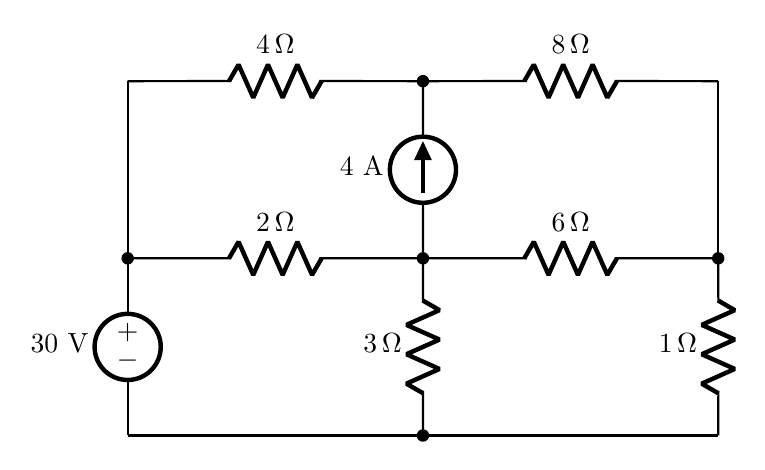
\begin{tikzpicture}[thick, scale=1.5]

    % Coordinates for the grid structure
    % Bottom row: (0,0), (2.5,0), (5,0)
    % Middle row: (0,1.5), (2.5,1.5), (5,1.5)
    % Top row:    (0,3), (2.5,3), (5,3)

    % Bottom wire line connection
    \draw (0,0) -- (5,0);

    % --- LEFT COLUMN ---
    % 30V Independent DC Voltage Source
    \draw (0,1.5) to[V, l_=$30\text{ V}$] (0,0);
    % Vertical connecting line from middle to top left
    \draw (0,1.5) -- (0,3);

    % --- MIDDLE COLUMN (Verticals) ---
    % Bottom vertical: 3 ohm resistor
    \draw (2.5,0) to[R, l=$3\,\Omega$] (2.5,1.5);
    % Top vertical: 4A Independent Current Source (pointing up)
    \draw (2.5,1.5) to[I, l=$4\text{ A}$] (2.5,3);

    % --- RIGHT COLUMN (Verticals) ---
    % Bottom right vertical: 1 ohm resistor
    \draw (5,0) to[R, l=$1\,\Omega$] (5,1.5);
    % Vertical connecting line from middle to top right
    \draw (5,1.5) -- (5,3);

    % --- HORIZONTAL ELEMENTS ---
    % Top Row
    \draw (0,3) to[R, l=$4\,\Omega$] (2.5,3)
                to[R, l=$8\,\Omega$] (5,3);

    % Middle Row
    \draw (0,1.5) to[R, l=$2\,\Omega$] (2.5,1.5)
                  to[R, l=$6\,\Omega$] (5,1.5);

    % Junction Nodes for Clarity
    \fill (0,1.5) circle (1.5pt);
    \fill (2.5,1.5) circle (1.5pt);
    \fill (5,1.5) circle (1.5pt);
    \fill (2.5,3) circle (1.5pt);
    \fill (2.5,0) circle (1.5pt);

\end{tikzpicture}

\end{center}
\mk{15} \yr{EEE 163 | L-1/T-1 | 2021--22}

\item Using mesh-current analysis, compute the current $i_o$ for the circuit shown below.
\begin{center}
  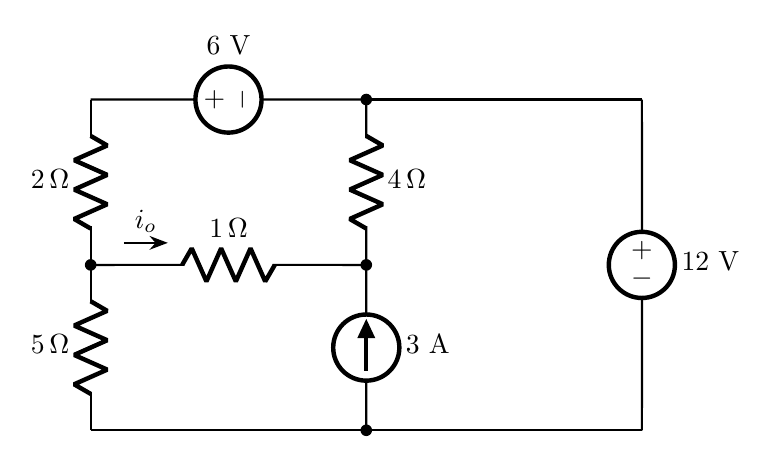
\begin{tikzpicture}[thick, american, scale=1.4]
    
    % Bottom reference rail
    \draw (0,0) -- (5,0);
    
    % Leftmost branch with 5 ohm and 2 ohm resistors split by a middle junction
    \draw (0,0) to[R, l=$5\,\Omega$] (0,1.5)
                to[R, l=$2\,\Omega$] (0,3);
                
    % Top independent voltage source (6V)
    \draw (0,3) to[V, l=$6\text{ V}$] (2.5,3);
    
    % Connection from 6V source to the rightmost branch
    \draw (2.5,3) -- (5,3);
    
    % Central horizontal branch with 1 ohm resistor and current indicator io
    \draw (0,1.5) to[R, l=$1\,\Omega$] (2.5,1.5);
    \draw[-{Stealth}, thick] (0.3,1.7) -- (0.7,1.7) node[midway, above] {$i_o$};
    
    % Middle vertical branches connecting to the central node (2.5, 1.5)
    \draw (2.5,3) to[R, l=$4\,\Omega$] (2.5,1.5);
    \draw (2.5,0) to[I, l_=$3\text{ A}$] (2.5,1.5);
    
    % Rightmost branch with 12V independent voltage source
    \draw (5,3) to[V, l=$12\text{ V}$] (5,0);

    % Explicit junction connection dots
    \fill (0,1.5) circle (1.5pt);
    \fill (2.5,3) circle (1.5pt);
    \fill (2.5,1.5) circle (1.5pt);
    \fill (2.5,0) circle (1.5pt);

\end{tikzpicture}

\end{center}
\mk{15} \yr{EEE 163 | L-1/T-1 | 2020--21}

\item In solving for currents using mesh analysis, the following equations are obtained. Draw the circuit and find the currents:
\begin{align*}
15i_1 - 10i_2 &= -10\\
10i_1 - 22i_2 + 10i_3 &= 0\\
10i_2 - 15i_3 &= 12
\end{align*}
\mk{12} \yr{EEE 163 | L-1/T-1 | 2018--19}

\item Using mesh current analysis, find the power delivered/absorbed by the 5\,A current source in the circuit below.
\begin{center}
  \begin{circuitikz}[thick, scale=1.2]
    % --- Ground/Bottom Wire ---
    \draw (0,0) -- (8,0);

    % --- Left Section ---
    % 1A independent current source and 2 ohm resistor
    \draw (0,0) to[I, l=$1\text{A}$] (0,2)
          to[R, l=$2\,\Omega$] (2,2);
          
    % 6 ohm vertical parallel resistor
    \draw (2,2) to[R, l=$6\,\Omega$] (2,0);

    % --- Middle Section ---
    % 4 ohm horizontal resistor
    \draw (2,2) to[R, l=$4\,\Omega$] (4,2);
          
    % 3I_o dependent current source (pointing down)
    \draw (4,2) to[cI, l=$3I_o$] (4,0);

    % 5A independent current source (pointing right)
    \draw (4,2) to[I, l=$5\text{A}$] (6,2);

    % --- Overhead Bridge ---
    % 2 ohm resistor bypassing the 5A source
    \draw (4,2) -- (4,3.2)
          to[R, l=$2\,\Omega$] (6,3.2)
          -- (6,2);

    % --- Right Section ---
    % 8 ohm vertical parallel resistor
    \draw (6,2) to[R, l=$8\,\Omega$] (6,0);

    % 2 ohm horizontal resistor leading to the final stage
    \draw (6,2) to[R, l=$2\,\Omega$] (8,2);

    % 10V independent voltage source with upward current I_o
    \draw (8,0) to[V, invert,l_=$10\text{V}$, i>=$I_o$] (8,2);

\end{circuitikz}

\end{center}
\mk{18} \yr{EEE 163 | L-1/T-1 | 2015--16}

\item Find $I_0$ and $V_0$ using mesh analysis for the circuit shown below.
\begin{center}
  \begin{circuitikz}[scale=1.3, transform shape, thick]

    % Far left branch: 1A independent current source
    \draw (0,0) to[I, l=$1\mathrm{A}$] (0,3) -- (2,3);

    % First parallel branch: 4 Ohm resistor
    \draw (2,0) to[R, l=$4\,\Omega$] (2,3);

    % Top bypass branch: 1 Ohm resistor with voltage V_o (+ on left)
    \draw (2,3) -- (2,4.5) to[R, l=$1\,\Omega$, v=$V_o$] (7.5,4.5) -- (7.5,3);

    % Middle horizontal branch: 2A independent current source pointing right
    \draw (2,3) to[I, l=$2\mathrm{A}$] (5,3);

    % Middle vertical branch: 1 Ohm resistor & dependent voltage source (4 I_0)
    % Drawing top-to-bottom places the + polarity on top by default
    \draw (5,3) to[R, l=$1\,\Omega$] (5,1.5)
                to[cV, l=$4I_0$] (5,0);

    % Middle-right horizontal branch: Dependent current source (2 V_o) pointing left
    % Drawing from 7.5 to 5 makes the arrow point left
    \draw (7.5,3) to[cI, l_=$2V_o$] (5,3);

    % Right vertical branch: 4 Ohm resistor with downward current I_0
    \draw (7.5,3) to[R, l=$4\,\Omega$, i=$I_0$] (7.5,0);

    % Rightmost branch: 2 Ohm series resistor and 10V independent voltage source
    \draw (7.5,3) to[R, l=$2\,\Omega$] (10,3) 
                to[V, l=$10\mathrm{V}$] (10,0);

    % Bottom ground/return wire connecting all branches
    \draw (0,0) -- (10,0);

    % Ground symbol at the middle branch
    \draw (5,0) node[ground]{};
\end{circuitikz}

\end{center}
\mk{17} \yr{EEE 163 | L-1/T-1 | 2014--15}

\item Determine $v_1$ and $i_1$ in the circuit below using mesh analysis.
\begin{center}
  \begin{circuitikz}[thick, scale=1.2, transform shape]

    % Leftmost branch
    \draw (0,2) to[V, l_=$5V$] (0,0);
    \draw (0,2) -- (0,4);

    % Top horizontal branch
    \draw (0,4) to[short, i=$i_1$] (1.5,4) 
          to[R, l=$7\Omega$] (3.5,4) 
          to[V, l=$3V$] (6,4);
    \draw (6,4) -- (6,2);

    % Middle horizontal branches
    \draw (0,2) to[R, l_=$5\Omega$] (3,2);
    \draw (6,2) to[cI, l=$0.5i_1$] (3,2); % Path from right to left puts arrow pointing left

    % Middle vertical branch
    \draw (3,2) to[cV, l_=$2v_1$] (3,0); % First coordinate is top, so + is on top

    % Bottom horizontal branches
    \draw (0,0) to[R, l_=$5\Omega$] (3,0);
    \draw (3,0) to[R, l_=$5\Omega$] (6,0);
    \draw (6,0) -- (8,0);

    % Right vertical branch
    \draw (6,2) to[R, l=$3\Omega$] (6,0); % v_ places voltage polarity on the left side of path

    % Far right branch
    \draw (6,2) to[R, l=$4\Omega$, v_=$v_1$] (8,2);
    \draw (8,0) to[I, l_=$5A$] (8,2); % Path from bottom to top puts arrow pointing up

    % Connection dots at junctions
    \node[circle, fill, inner sep=1.2pt] at (0,2) {};
    \node[circle, fill, inner sep=1.2pt] at (3,2) {};
    \node[circle, fill, inner sep=1.2pt] at (6,2) {};
    \node[circle, fill, inner sep=1.2pt] at (3,0) {};
    \node[circle, fill, inner sep=1.2pt] at (6,0) {};


\end{circuitikz}

\end{center}
\mk{18} \yr{EEE 163 | L-1/T-1 | 2013--14}

\item Use mesh-current method to determine the branch currents $i_a$, $i_b$ and the power associated with each source in the circuit shown below.
\begin{center}
  \begin{circuitikz}[thick,scale=1.2, transform shape]
    % Bottom reference wire
    \draw (0,0) -- (8,0);
    
    % Leftmost branch: 15A independent current source pointing upwards
    \draw (0,0) to[I, l=15~A] (0,3) -- (2,3);
    
    % First vertical parallel branch: 40 ohm resistor with downward current ia
    \draw (2,3) to[R, l=40~$\Omega$, i=$i_a$] (2,0);
    
    % Top middle horizontal branch: 5 ohm resistor with current ib pointing left
    % (Drawn from right to left to orient the current arrow correctly)
    \draw (5,3) to[R, l=5~$\Omega$, i=$i_b$] (2,3);
    
    % Middle vertical branch: Dependent current source (2*ib) pointing upwards
    \draw (5,0) to[cI, l=2$i_b$] (5,3);
    
    % Top right horizontal branch: 10 ohm resistor
    \draw (5,3) to[R, l=10~$\Omega$] (8,3);
    
    % Rightmost vertical branch: 240V independent voltage source 
    % (Drawn from top to bottom to put the - terminal on top and + on bottom)
    \draw (8,3) to[V, l=240~V] (8,0);
    
    % Connection dots at main circuit junctions
    \node[circle, fill, inner sep=1.5pt] at (2,3) {};
    \node[circle, fill, inner sep=1.5pt] at (5,3) {};
    
\end{circuitikz}

\end{center}
\mk{15} \yr{EEE 163 | L-1/T-1 | 2012--13}

\item Use the mesh-current method to find the power developed in the dependent voltage source in the circuit shown below.
\begin{center}
  \begin{circuitikz}[american , thick]
    % --- Middle Horizontal Rail ---
    \draw (0,2.5) to[R, l={3 $\Omega$}] (3.5,2.5)
          to[R, l={5 $\Omega$}] (7,2.5);

    % --- Left Vertical Branch (30V independent source: - on top, + on bottom) ---
    \draw (0,0) to[V, l={30 V}] (0,2.5);

    % --- Bottom Horizontal Rail ---
    \draw (0,0) to[R, l_={7 $\Omega$}] (3.5,0)
          to[R, l_={2 $\Omega$}] (7,0);

    % --- Right Vertical Branch (30V independent source: + on top, - on bottom) ---
    \draw (7,2.5) to[V, invert,l={30 V}] (7,0);

    % --- Center Vertical Branch (20 Ohm resistor with manual current arrow) ---
    \draw (3.5,2.5) to[R, l={20 $\Omega$}] (3.5,0);
    \draw[->, >=stealth, thick] (3.1, 1.6) -- (3.1, 0.9) node[midway, left] {$i_{20}$};

    % --- Topmost Branch (Dependent Voltage Source: + on left, - on right) ---
    \draw (0,2.5) -- (0,4.5)
          to[cV, l={$53 i_{20}$}] (7,4.5)
          -- (7,2.5);
\end{circuitikz}

\end{center}
\mk{25} \yr{EEE 163 | L-1/T-1 | 2011--12}

\item Using mesh analysis, find the value of $V_0$ in the circuit shown below.
\begin{center}
  \begin{circuitikz}[thick,american]
    
    % Bottom wire connecting all branches
    \draw (0,0) -- (11,0);

    % Leftmost branch: 12V voltage source
    % 'invert' is used so the positive terminal (+) is at the top
    \draw (0,0) to[V, l=$12\text{V}$, invert] (0,4);

    % Top wire, part 1: 2 ohm resistor
    \draw (0,4) to[R, l=$2\,\Omega$] (4,4);

    % First middle branch: 2A current source (arrow points down)
    \draw (4,4) to[I, l=$2\text{A}$] (4,0);

    % Top wire, part 2: 1 ohm resistor
    \draw (4,4) to[R, l=$1\,\Omega$] (8,4);

    % Second middle branch: 6V source and 2 ohm resistor with V_0
    % Drawing from top to bottom places the (+) of 6V at the top.
    % 'v=$V_0$' automatically adds the +/- polarity markings across the resistor.
    \draw (8,4) to[V, l=$6\text{V}$] (8,2)
          to[R, l=$2\,\Omega$, v=$V_0$] (8,0);

    % Top wire, part 3: 4V voltage source
    % Drawing left to right places the (+) at the left node (8,4)
    \draw (8,4) to[V, l=$4\text{V}$] (11,4);

    % Rightmost branch: 1 ohm resistor
    \draw (11,4) to[R, l=$1\,\Omega$] (11,0);

    % Add connection dots at the key nodes
    \node[circ] at (4,4) {};
    \node[circ] at (8,4) {};
    \node[circ] at (4,0) {};
    \node[circ] at (8,0) {};

\end{circuitikz}
\end{center}
\mk{17} \yr{EEE 163 | L-1/T-1 | 2010--11}

\item Determine the power absorbed by the 1.5\,A current source in the circuit below using mesh analysis.
\begin{center}
  \begin{circuitikz}[thick ,american, scale=1.2, transform shape]
    
    % Define the main coordinate points
    \coordinate (BL) at (0,0);
    \coordinate (BC) at (4,0);
    \coordinate (BR) at (8,0);
    \coordinate (TL) at (0,7);
    \coordinate (TC) at (4,7);
    \coordinate (TR) at (8,7);
    \coordinate (C)  at (4,3.5);
    
    % Bottom Wire with connection dots
    \draw (BL) -- (BR);
    \node[circ] at (BL) {};
    \node[circ] at (BC) {};
    \node[circ] at (BR) {};
    
    % Left Vertical Branch (2V Source and 10 Ohm Resistor)
    \draw (BL) to[V,invert, l=$2\text{V}$] (0,3.5) to[R, l=$10\Omega$] (TL);
    \node[circ] at (TL) {};
    
    % Right Vertical Branch (3V Source and 15 Ohm Resistor)
    \draw (BR) to[V,invert, l_=$3\text{V}$] (8,3.5) to[R, l_=$15\Omega$] (TR);
    \node[circ] at (TR) {};
    
    % Top Horizontal Branches (20 Ohm and 15 Ohm Resistors)
    \draw (TL) to[R, l=$20\Omega$] (TC);
    \draw (TC) to[R, l=$15\Omega$] (TR);
    \node[circ] at (TC) {};
    
    % Diagonal Branches
    % Left diagonal with voltage v_0 annotation
    \draw (TL) to[R, l_=$15\Omega$, v^=$v_0$] (C);
    % Right diagonal
    \draw (C) to[R, l_=$10\Omega$] (TR);
    \node[circ] at (C) {};
    
    % Center Vertical Branches
    % Bottom part: 1.5A Independent Current Source and 15 Ohm Resistor
    \draw (BC) to[I, l_=$1.5\text{A}$] (4,1.75) to[R, l_=$15\Omega$] (C);
    % Top part: 10 Ohm Resistor and 0.1v_0 Dependent Current Source
    \draw (C) to[R, l_=$10\Omega$] (4,5.25) to[cI, l_=$0.1v_0$] (TC);

\end{circuitikz}

\end{center}
\mk{18} \yr{EEE 163 | L-1/T-1 | 2008--09}

\item Determine the loop currents for the circuit shown below using Mesh Current Analysis method.
\begin{center}
  
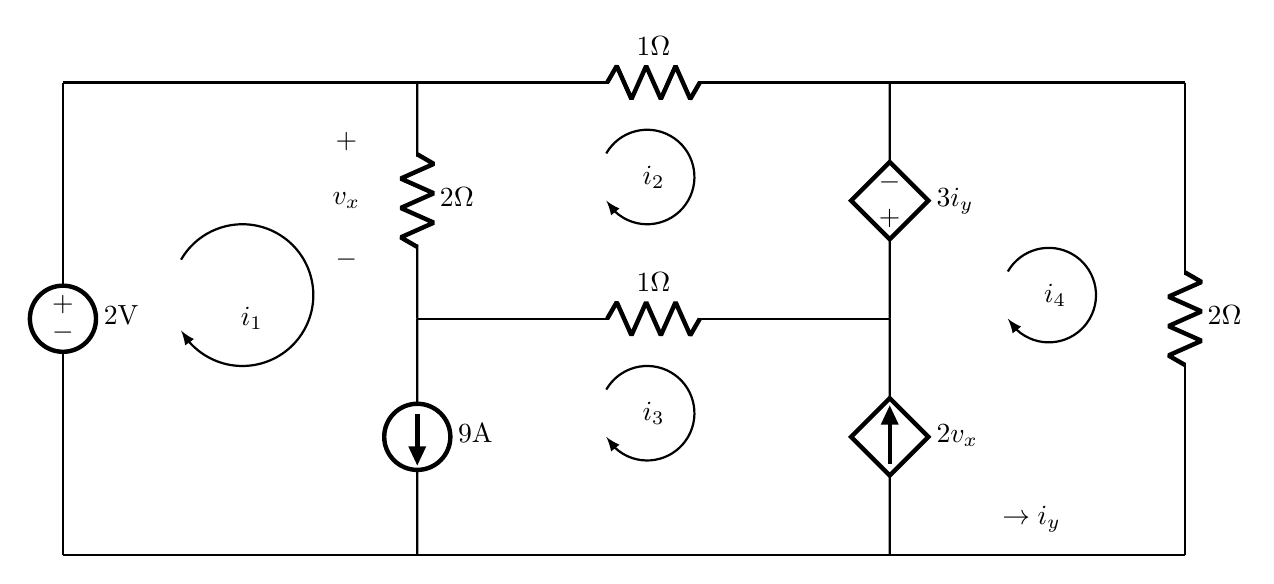
\begin{tikzpicture}[american, thick ,x=1.5cm,y =1.5cm]

    % --- Leftmost Branch ---
    \draw (0,4) to[V, l=$2\text{V}$] (0,0);
    
    % --- Top & Bottom Horizontal Wires (Left Pane) ---
    \draw (0,4) -- (3,4);
    \draw (0,0) -- (3,0);
    
    % --- Middle-Left Branch ---
    \draw (3,4) to[R, l=$2\Omega$] (3,2);
    \draw (3,2) to[I, l=$9\text{A}$] (3,0);
    
    % v_x polarity labels (Manual placement for exact matching)
    \node at (2.4, 3.5) {$+$};
    \node at (2.4, 3.0) {$v_x$};
    \node at (2.4, 2.5) {$-$};
    
    % --- Middle Horizontal Wire ---
    \draw (3,2) to[R, l=$1\Omega$] (7,2);
    
    % --- Top Horizontal Wire (Middle Pane) ---
    \draw (3,4) to[R, l=$1\Omega$] (7,4);
    
    % --- Bottom Horizontal Wire (Middle Pane) ---
    \draw (3,0) -- (7,0);
    
    % --- Middle-Right Branch ---
    % Dependent Voltage Source (+ on top)
    \draw (7,2) to[cV, l_=$3i_y$] (7,4);
    % Dependent Current Source (Arrow UP)
    \draw (7,0) to[cI, l_=$2v_x$] (7,2);
    
    % --- Top & Bottom Horizontal Wires (Right Pane) ---
    \draw (7,4) -- (9.5,4);
    \draw (7,0) -- (9.5,0);
    
    % --- Rightmost Branch ---
    \draw (9.5,4) to[R, l=$2\Omega$] (9.5,0);
    
    % --- i_y label on bottom right ---
    \node at (8.2, 0.3) {$\rightarrow i_y$};
    
    % --- Mesh Currents (Clockwise Loops) ---
    % Mesh i1
    \draw[-latex] (1.0, 2.5) arc (150:-150:0.6);
    \node at (1.6, 2.0) {$i_1$};
    
    % Mesh i2
    \draw[-latex] (4.6, 3.4) arc (150:-150:0.4);
    \node at (5, 3.2) {$i_2$};
    
    % Mesh i3
    \draw[-latex] (4.6, 1.4) arc (150:-150:0.4);
    \node at (5, 1.2) {$i_3$};
    
    % Mesh i4
    \draw[-latex] (8.0, 2.4) arc (150:-150:0.4);
    \node at (8.4, 2.2) {$i_4$};


\end{tikzpicture}
\end{center}
\mk{20} \yr{EEE 163 | L-1/T-1 | 2007--08}

\item Determine the voltage, $v$ and the current, $I$ using Mesh Analysis for the circuit shown below.
\begin{center}
  \begin{circuitikz}[thick, y=1.2cm]

    % ---------------------------------------------------
    % Top Bridge Loop
    % ---------------------------------------------------
    % 3 Ohm vertical resistor going up
    \draw (3,4) to[R, l=$3\Omega$] (3,5.5);
    % 3A source (drawn right-to-left so arrow points left)
    \draw (7,5.5) to[I, l_=$3\text{A}$] (3,5.5);
    \draw (7,5.5) -- (7,4);

    % ---------------------------------------------------
    % Main Horizontal Top Branches
    % ---------------------------------------------------
    \draw (0,4) to[R, l=$2\Omega$] (3,4);
    \draw (3,4) to[R, l_=$2\Omega$] (5,4);
    
    % 4 Ohm resistor with text below, and manual - V + above it
    \draw (5,4) to[R, l_=$4\Omega$] (7,4);
    \node at (5.4, 4.6) {$-$};
    \node at (6.0, 4.6) {$V$};
    \node at (6.6, 4.6) {$+$};

    \draw (7,4) to[R, l=$1\Omega$] (9,4);
    \draw (9,4) -- (11,4);

    % ---------------------------------------------------
    % Vertical Branches
    % ---------------------------------------------------
    % Leftmost 20V Source (drawn top-to-bottom so + is on top)
    \draw (0,4) to[V,invert, l_=$20\text{V}$] (0,1);
    
    % Middle Branch (3 Ohm & 3V Source)
    \draw (7,4) to[R, l=$3\Omega$] (7,2.5);
    % 3V Source (drawn top-to-bottom so + is on top)
    \draw (7,2.5) to[V,invert, l=$3\text{V}$] (7,1);
    
    % Rightmost inner branch (1 Ohm with a jump over the horizontal line)
    \draw (9,4) to[R, l_=$1\Omega$] (9,1.2);
    % Jump arc over the y=1 horizontal line
    \draw (9,1.2) arc[start angle=90, end angle=-90, radius=0.2];
    \draw (9,0.8) -- (9,0);
    
    % Far right vertical branch (3 Ohm)
    \draw (11,4) to[R, l=$3\Omega$] (11,1);

    % ---------------------------------------------------
    % Horizontal Return Lines
    % ---------------------------------------------------
    % Main middle return line
    \draw (0,1) -- (11,1);

    % Bottom-most loop (y=0 line)
    \draw (9,0) -- (6.5,0);
    \draw (6.5,0) to[R, l=$2\Omega$] (4.5,0);
    % 10V Source (drawn right-to-left so + is on right, - is on left)
    \draw (4.5,0) to[V, l=$10\text{V}$] (2.5,0);
    % Wire with Current I pointing left
    \draw (2.5,0) to[short, i_=$I$] (0,0);
    
    % Connect bottom loop back up to the main corner
    \draw (0,0) -- (0,1);

    % ---------------------------------------------------
    % Junction Nodes (Dots)
    % ---------------------------------------------------
    \node[circ] at (3,4) {};
    \node[circ] at (7,4) {};
    \node[circ] at (9,4) {};
    \node[circ] at (0,1) {};
    \node[circ] at (7,1) {};
    % ---------------------------------------------------
    % Figure Label
    % ---------------------------------------------------

\end{circuitikz}
\end{center}
\mk{17} \yr{EEE 163 | L-1/T-1 | 2006--07}

\item For the circuit shown below, find the currents $I_1$ and $I_2$ using loop current method. Also find the power supplied by the 5\,A current source.
\begin{center}
  
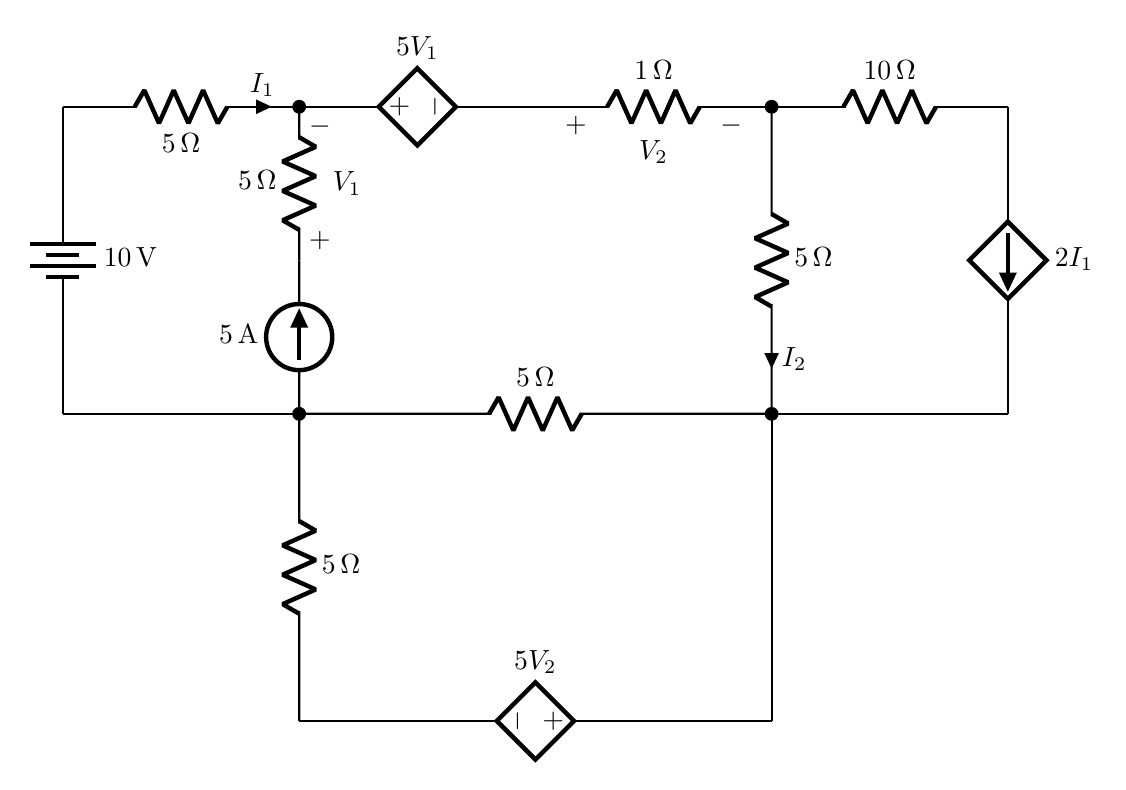
\begin{tikzpicture}[thick, y=1.3cm, >=stealth]

    % --- Leftmost Loop ---
    % 10V Battery drawn bottom-up so positive (long plate) is on top
    \draw (0,6) to[battery, l=$10\,\text{V}$] (0,3);
    % Top wire with 5 Ohm resistor and current I1
    % l_ places the 5 Ohm label below, i places I1 above
    \draw (0,6) to[R, l_=$5\,\Omega$, i=$I_1$] (3,6);
    \draw (0,3) -- (3,3); % Bottom return wire for this section

    % --- First Vertical Branch (x = 3) ---
    % 5 Ohm resistor with explicit V1 polarity (+ on top, - on bottom)
    \draw (3,4.5) to[R, l=$5\,\Omega$, v=$V_1$] (3,6);
    % 5A independent current source drawn bottom-up for upward arrow
    \draw (3,3) to[I, l=$5\,\text{A}$] (3,4.5);

    % --- Top Horizontal Branches (x = 3 to 9) ---
    % Dependent voltage source 5V_1
    \draw (3,6) to[cV, l=$5V_1$] (6,6); 
    % 1 Ohm resistor with V2 polarity (+ on left, - on right)
    \draw (6,6) to[R, l=$1\,\Omega$, v=$V_2$] (9,6);

    % --- Middle Horizontal Branch ---
    \draw (3,3) to[R, l=$5\,\Omega$] (9,3);

    % --- Second Vertical Branch (x = 9) ---
    % 5 Ohm resistor with downward current I2
    \draw (9,6) to[R, l=$5\,\Omega$, i=$I_2$] (9,3);

    % --- Rightmost Loop (x = 9 to 12) ---
    \draw (9,6) to[R, l=$10\,\Omega$] (12,6);
    % Dependent current source 2I_1 drawn top-down for downward arrow
    \draw (12,6) to[cI, l=$2I_1$] (12,3); 
    \draw (12,3) -- (9,3);

    % --- Bottom Loop ---
    \draw (3,3) to[R, l=$5\,\Omega$] (3,0);
    % Dependent voltage source 5V_2 drawn left-right for standard polarity
    \draw (9,0) to[cV, l_=$5V_2$] (3,0); 
    \draw (9,0) -- (9,3);

    % --- Explicit Connection Junction Dots ---
    \fill (3,6) circle (2.5pt);
    \fill (3,3) circle (2.5pt);
    \fill (9,6) circle (2.5pt);
    \fill (9,3) circle (2.5pt);


\end{tikzpicture}
\end{center}
\mk{18} \yr{EEE 163 | L-1/T-1 | 2005--06}

\end{enumerate}

%%──────────────────────────────────────────────────────────────────────
\subtopic{cA}{Nodal Analysis}
\label{sub:s1-nodal}

\begin{enumerate}

\item For the circuit shown below for Question 3(a), use an appropriate analysis technique to 
find the voltage across the $2 \; \Omega$ resistor. Use Cramer's rule to solve the circuit equations.
\begin{center}
  \begin{circuitikz}[scale=1.3, transform shape, thick]

    % Far left branch: 1A independent current source
    \draw (0,0) to[I, l=$1\mathrm{A}$] (0,3) -- (2,3);

    % First parallel branch: 4 Ohm resistor
    \draw (2,0) to[R, l=$4\,\Omega$] (2,3);

    % Top bypass branch: 1 Ohm resistor with voltage V_o (+ on left)
    \draw (2,3) -- (2,4.5) to[R, l=$1\,\Omega$, v=$V_o$] (7.5,4.5) -- (7.5,3);

    % Middle horizontal branch: 2A independent current source pointing right
    \draw (5,3) to[cV, l=$4I_o$] (2,3);

    % Middle vertical branch: 1 Ohm resistor & dependent voltage source (4 I_0)
    % Drawing top-to-bottom places the + polarity on top by default
    \draw (5,3) to[R, l=$1\,\Omega$]  (5,0);

    % Middle-right horizontal branch: Dependent current source (2 V_o) pointing left
    % Drawing from 7.5 to 5 makes the arrow point left
    \draw (7.5,3) to[cI, l_=$2V_o$] (5,3);

    % Right vertical branch: 4 Ohm resistor with downward current I_0
    \draw (7.5,3) to[R, l=$4\,\Omega$, i=$I_0$] (7.5,0);

    % Rightmost branch: 2 Ohm series resistor and 10V independent voltage source
    \draw (7.5,3) to[R, l=$2\,\Omega$] (10,3) 
                to[V, l=$10\mathrm{V}$] (10,0);

    % Bottom ground/return wire connecting all branches
    \draw (0,0) -- (10,0);

    % Ground symbol at the middle branch
    \draw (5,0) node[ground]{};
\end{circuitikz}

\end{center}
\mk{20} \yr{EEE 163 | L-1/T-1 | 2024--25}


  \item For the circuit shown below, use the node analysis method to find the power dissipated in the 300\,$\Omega$ resistor. You must use the reference node as shown in the figure.
  \begin{center}
  \begin{circuitikz}[thick,american, scale=1.2, transform shape]

    % Bottom wire with junction dots
    \draw (0,0) -- (2,0) node[circ]{} -- (5,0) node[circ]{} -- (8,0) node[circ]{} -- (10,0);
    
    % Node label v3 at the bottom

    % Leftmost independent voltage source (256V)
    \draw (0,3) to[V, l=$256\text{ V}$] (0,0);

    % Top horizontal main branches
    \draw (0,3) to[R, l=$150\ \Omega$] (2,3) node[circ]{0V};
    \draw (2,3) to[R, l=$100\ \Omega$] (5,3) node[circ]{};
     
    \draw (5,3) to[R, l=$250\ \Omega$] (8,3) node[circ]{};
    \draw (8,3) to[R, l=$500\ \Omega$] (10,3);

    % Vertical elements
    % 200 Ohm Resistor
    \draw (2,3) to[R, l=$200\ \Omega$] (2,0);
    
    % Dependent Voltage Source (50 i_\Delta) - Drawn bottom to top for + on top
    \draw (5,3) to[cV, l=$50\ i_\Delta$] (5,0);
    
    % 400 Ohm Resistor
    \draw (8,3) to[R, l=$400\ \Omega$] (8,0);
    
    % Rightmost independent voltage source (128V) - Drawn top to bottom for - on top
    \draw (10,0) to[V, l_=$128\text{ V}$] (10,3);

    % Top bridge branch with 300 Ohm Resistor
    \draw (2,3) -- (2,4.5) to[R, l=$300\ \Omega$] (8,4.5) -- (8,3);
    
    % Current arrow i_\Delta pointing left above the 300 Ohm resistor
    \draw[latex-] (6, 4.9) -- (7, 4.9) node[midway, above] {$i_\Delta$};


\end{circuitikz}
\end{center}
\mk{20} \yr{EEE 163 | L-1/T-1 | 2023--24}

\item Use Node Analysis technique to find the power dissipated in the 300\,$\Omega$ resistor in the circuit shown below.
\begin{center}
  \begin{circuitikz}[thick, american, scale=1.2, transform shape]

    % Bottom wire with junction dots
    \draw (0,0) -- (2,0) node[circ]{} -- (5,0) node[circ]{} -- (8,0) node[circ]{} -- (10,0);
    
    % Node label v3 at the bottom

    % Leftmost independent voltage source (256V)
    \draw (0,3) to[V, l=$256\text{ V}$] (0,0);

    % Top horizontal main branches
    \draw (0,3) to[R, l=$150\ \Omega$] (2,3) node[circ]{};
    \draw (2,3) to[R, l=$100\ \Omega$] (5,3) node[circ]{};
     
    \draw (5,3) to[R, l=$250\ \Omega$] (8,3) node[circ]{};
    \draw (8,3) to[R, l=$500\ \Omega$] (10,3);

    % Vertical elements
    % 200 Ohm Resistor
    \draw (2,3) to[R, l=$200\ \Omega$] (2,0);
    
    % Dependent Voltage Source (50 i_\Delta) - Drawn bottom to top for + on top
    \draw (5,3) to[cV, l=$50\ i_\Delta$] (5,0);
    
    % 400 Ohm Resistor
    \draw (8,3) to[R, l=$400\ \Omega$] (8,0);
    
    % Rightmost independent voltage source (128V) - Drawn top to bottom for - on top
    \draw (10,0) to[V, l_=$128\text{ V}$] (10,3);

    % Top bridge branch with 300 Ohm Resistor
    \draw (2,3) -- (2,4.5) to[R, l=$300\ \Omega$] (8,4.5) -- (8,3);
    
    % Current arrow i_\Delta pointing left above the 300 Ohm resistor
    \draw[latex-] (6, 4.9) -- (7, 4.9) node[midway, above] {$i_\Delta$};


\end{circuitikz}
\end{center}
\mk{17} \yr{EEE 163 | L-1/T-1 | 2022--23, 2017--18}

\item Use nodal analysis to find the current through the 12\,V source as shown below and determine whether the 12\,V source is supplying or absorbing power.
\begin{center}
  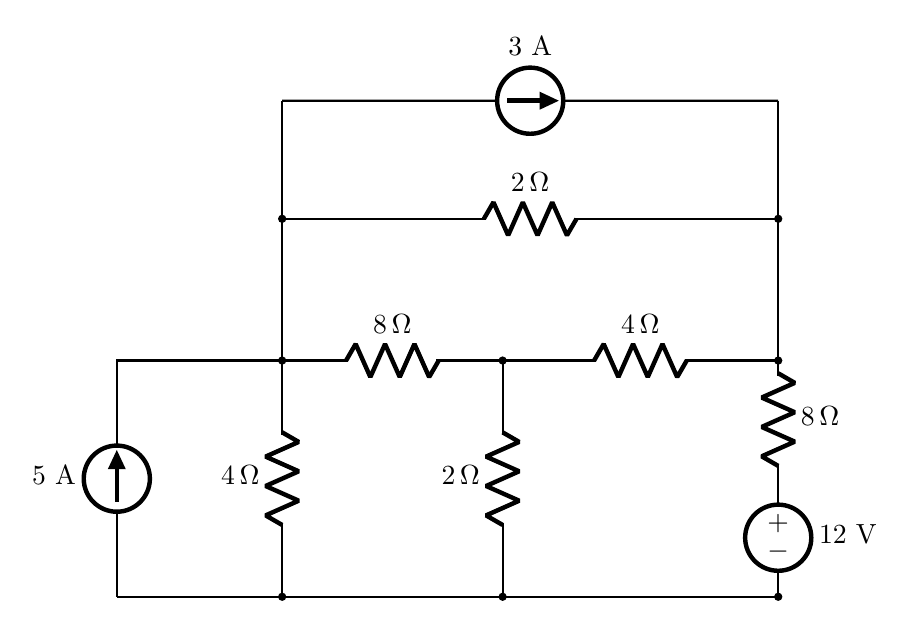
\begin{tikzpicture}[thick, y=1.5cm,x=1.4cm]

    % --- BASE CONNECTIONS ---
    % Bottom ground reference line
    \draw (0,0) -- (6,0); 

    % --- LEFTMOST VERTICAL BRANCH ---
    % 5A Current Source
    \draw (0,0) to[I, l=$5\text{ A}$] (0,2) -- (1.5,2);

    % --- RECTANGULAR GRID LAYER 1 ---
    % 4 ohm resistor (vertical)
    \draw (1.5,0) to[R, l=$4\,\Omega$] (1.5,2);
    
    % 2 ohm resistor (center vertical)
    \draw (3.5,0) to[R, l=$2\,\Omega$] (3.5,2);
    
    % Rightmost vertical branch with 8 ohm resistor and 12V source
    \draw (6,0) to[V,invert,  l_=$12\text{ V}$] (6,1)
                to[R, l_=$8\,\Omega$] (6,2);

    % --- HORIZONTAL ELEMENTS (MIDDLE ROW) ---
    \draw (1.5,2) to[R, l=$8\,\Omega$] (3.5,2)
                  to[R, l=$4\,\Omega$] (6,2);

    % --- UPPER OVERHEAD BRIDGES ---
    % Node connections extending upwards
    \draw (1.5,2) -- (1.5,3.2);
    \draw (6,2)   -- (6,3.2);

    % First upper bridge: 2 ohm resistor
    \draw (1.5,3.2) to[R, l=$2\,\Omega$] (6,3.2);

    % Node extensions to the topmost layer
    \draw (1.5,3.2) -- (1.5,4.2);
    \draw (6,3.2)   -- (6,4.2);

    % Topmost bridge: 3A Current Source (pointing right)
    \draw (1.5,4.2) to[I, l=$3\text{ A}$] (6,4.2);

    % --- JUNCTION DOTS ---
    \fill (1.5,2) circle (1.5pt);
    \fill (3.5,2) circle (1.5pt);
    \fill (6,2)   circle (1.5pt);
    \fill (1.5,3.2) circle (1.5pt);
    \fill (6,3.2)   circle (1.5pt);
    \fill (1.5,0) circle (1.5pt);
    \fill (3.5,0) circle (1.5pt);
    \fill (6,0)   circle (1.5pt);

\end{tikzpicture}

\end{center}
\mk{20} \yr{EEE 163 | L-1/T-1 | 2021--22}

\item Using node-voltage analysis, find the node voltages $v_1$, $v_2$, $v_3$ for the circuit shown below.
\begin{center}
  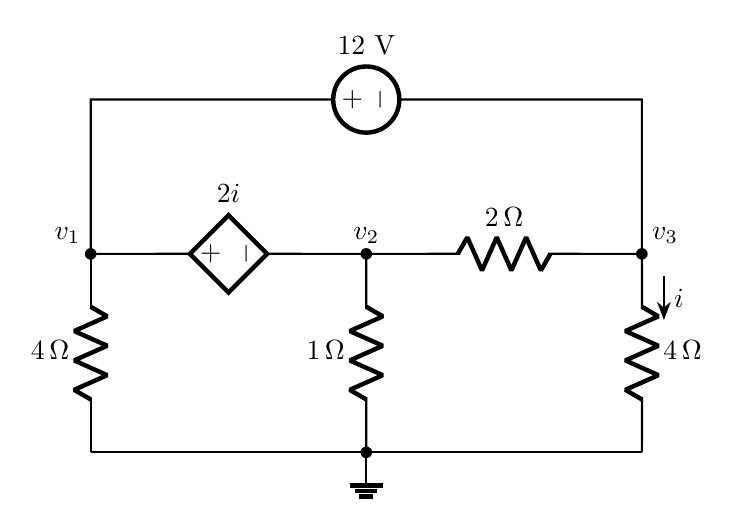
\begin{tikzpicture}[thick, american, scale=1.4]
    
    % Reference Ground rail at the bottom
    \draw (0,0) -- (5,0);
    \draw (2.5,0) node[ground] {};
    
    % First vertical branch: 4 ohm resistor on the left
    \draw (0,0) to[R, l=$4\,\Omega$] (0,1.8);
    
    % Central vertical branch: 1 ohm resistor connected to ground
    \draw (2.5,0) to[R, l=$1\,\Omega$] (2.5,1.8);
    
    % Right vertical branch: 4 ohm resistor with current i
    \draw (5,0) to[R, l_=$4\,\Omega$] (5,1.8);
    \draw[-{Stealth}, thick] (5.2,1.6) -- (5.2,1.2) node[midway, right] {$i$};
    
    % Middle horizontal line connections with nodes and components
    % Left segment: Dependent voltage source (2i)
    \draw (0,1.8) to[cV, l=$2i$] (2.5,1.8);
    
    % Right segment: 2 ohm resistor
    \draw (2.5,1.8) to[R, l=$2\,\Omega$] (5,1.8);
    
    % Top loop containing the independent 12V voltage source
    \draw (0,1.8) -- (0,3.2)
                  to[V, l=$12\text{ V}$] (5,3.2)
                  -- (5,1.8);
                  
    % Node voltage labels (v1, v2, v3)
    \node[above left] at (0,1.8) {$v_1$};
    \node[above] at (2.5,1.8) {$v_2$};
    \node[above right] at (5,1.8) {$v_3$};

    % Explicit junction connection dots
    \fill (0,1.8) circle (1.5pt);
    \fill (2.5,1.8) circle (1.5pt);
    \fill (2.5,0) circle (1.5pt);
    \fill (5,1.8) circle (1.5pt);

\end{tikzpicture}

\end{center}
\mk{20} \yr{EEE 163 | L-1/T-1 | 2020--21}

\item Determine the values of node voltages $V_1$, $V_2$, $V_3$, $V_4$ and the power of the dependent source for the circuit below.
\begin{center}
  \begin{circuitikz}[scale=1.2,thick,  every node/.style={transform shape}]

    % --- Bottom Reference Ground Rail ---
    \draw (0,0) to[short] (10,0);
    
    % --- Node V1 Area ---
    \draw (0,0) to[I, l=$3\,\text{A}$] (0,3)
          to[short] (1.5,3) node[above left] {$V_1$};
    \draw (1.5,3) to[R, l=$5\,\Omega$] (1.5,0);
    
    % --- Node V2 Area & Vertical Vx Branch ---
    \draw (4.5,3) node[above right] {$V_2$}
          to[R, l=$3\,\Omega$, v<=$V_x$] (4.5,0); % Note: Vx polarity has - at top, + at bottom
          
    % --- Node V3 Area ---
    \draw (7,3) node[above right] {$V_3$}
          to[V, l=$12\,\text{V}$] (7,0);

    % --- Node V4 Area ---
    \draw (10,3) node[above right] {$V_4$}
          to[I, l=$4\,\text{A}$] (10,0);

    % --- Horizontal Component Bridges ---
    % Dependent voltage source between V1 and V2
    \draw (4.5,3) to[cV, l=$3I_x$] (1.5,3);
    
    % Resistor between V2 and V3
    \draw (4.5,3) to[R, l_=$8\,\Omega$] (7,3);
    
    % Resistor between V3 and V4
    \draw (7,3) to[R, l_=$4\,\Omega$] (10,3);

    % --- Overhead Crossings & Dependent Sources ---
    
    % 1. Wire from V1 up to the dependent current source 2Vx, crossing over to Node V3
    \draw (1.5,3) -- (1.5,4.2)
          to[cI, l=$2V_x$] (5,4.2) 
          .. controls (6,4.2) and (6.8,3.7) .. (7,3);

    % 2. Wire from V2 looping over to the 6 Ohm resistor, leading into Node V4
    % Includes the Ix control current tracker pointing left
    \draw (4.5,3) .. controls (4.8,3.8) and (6.5,4.5) .. (7.5,4.2)
          to[R, l=$6\,\Omega$, i_<= $I_x$] (10,4.2) -- (10,3);

    % --- Connection Node Dots ---
    \node[circle, fill, inner sep=1.2pt] at (1.5,3) {};
    \node[circle, fill, inner sep=1.2pt] at (4.5,3) {};
    \node[circle, fill, inner sep=1.2pt] at (7,3) {};
    \node[circle, fill, inner sep=1.2pt] at (10,3) {};
    \node[circle, fill, inner sep=1.2pt] at (1.5,0) {};
    \node[circle, fill, inner sep=1.2pt] at (4.5,0) {};
    \node[circle, fill, inner sep=1.2pt] at (7,0) {};
    \node[circle, fill, inner sep=1.2pt] at (10,0) {};

\end{circuitikz}

\end{center}
\mk{17} \yr{EEE 163 | L-1/T-1 | 2018--19}

\item Find $I_o$ in the network shown below using nodal analysis.
\begin{center}
  \begin{circuitikz}[scale=1.2, thick ]

    % --- Main Ground Reference Bottom Rail ---
    \draw (0,0) to[short] (5.5,0);

    % --- Leftmost Vertical Branch: 1 kOhm Resistor ---
    \draw (0,0) to[R, l=$1\,\text{k}\Omega$] (0,2) coordinate (LeftMidNode);

    % --- Left Upper Branch: Dependent Voltage Source (5Vx) ---
    \draw (LeftMidNode) to[cV,invert, l=$5V_x$] (0,4)
                        to[short] (3,4) coordinate (TopMidNode);

    % --- Central Horizontal Stage: 1 kOhm Resistor tracking Vx ---
    \draw (LeftMidNode) to[R, l=$1\,\text{k}\Omega$, v=$V_x$] (3,2) coordinate (CenterMidNode);

    % --- Central Vertical Upper Branch: 2 mA Current Source ---
    \draw (CenterMidNode) to[I, l=$2\,\text{mA}$] (TopMidNode);

    % --- Central Vertical Lower Branch: 10V Independent Source ---
    \draw (CenterMidNode) to[V, l=$10\,\text{V}$] (3,0);

    % --- Rightmost Phase: 5 kOhm Load Branch with Current Io ---
    \draw (TopMidNode) to[short] (5.5,4)
                       to[R, l=$5\,\text{k}\Omega$, i=$I_o$] (5.5,0);
    % --- Connection Node Dots ---
    \node[circle, fill, inner sep=1.2pt] at (LeftMidNode) {};
    \node[circle, fill, inner sep=1.2pt] at (CenterMidNode) {};
    \node[circle, fill, inner sep=1.2pt] at (TopMidNode) {};

\end{circuitikz}

\end{center}
\mk{15} \yr{EEE 163 | L-1/T-1 | 2018--19}

\item Find the node voltages and current $I_0$ using nodal analysis for the circuit below.
\begin{center}
  \begin{circuitikz}[scale=1.3, transform shape, thick]

    % Define y-levels for precise alignment
    \def\ytop{3.5}
    \def\ymid{1.75}
    \def\ygnd{0}
    \def\ybot{-1.5}

    % Far left branch: Ground and 20V independent voltage source (+ on top)
    \draw (0,\ygnd) node[ground]{} to[V, l=$10\mathrm{V}$, invert] (0,\ytop);

    % Top left wire connecting to the middle-left branch
    \draw (0,\ytop) -- (2,\ytop);

    % Middle-left vertical branch: 10 Ohm and 20 Ohm resistors
    \draw (2,\ytop) to[cI, l_=$5I_{o}$] (2,\ymid);
    \draw (2,\ymid) to[R, l_=$2\,\Omega$] (2,\ybot);

    % Middle horizontal cross-branch: Current I_0 and 2V voltage source
    % I_0 arrow points left towards the 10/20 Ohm junction
    \draw (3.5,\ymid) to[short, i_=$I_0$] (2,\ymid);
    % 2V source with + on the left
    \draw (3.5,\ymid) to[V, l=$2\mathrm{V}$] (5.5,\ymid);

    % Middle-right vertical branch: Dependent current source and 2 Ohm resistor
    % Dependent current source pointing down
    \draw (5.5,\ytop) to[R, l=$10\Omega$] (5.5,\ymid);
    % 2 Ohm resistor connecting to ground
    \draw (5.5,\ymid) to[R, l=$2\,\Omega$] (5.5,\ygnd) node[ground]{};

    % Top right wire connecting the dependent source to the 10V source
    \draw (5.5,\ytop) -- (8,\ytop);

    % Far right branch: 10V independent voltage source (+ on top)
    \draw (8,\ytop) to[V, l=$20\mathrm{V}$] (8,\ybot);

    % Bottom return wire connecting the 20 Ohm resistor and the 10V source
    \draw (2,\ybot) -- (8,\ybot);

    % Add connection dots at the main junctions
    \draw (2,\ymid) node[circ]{};
    \draw (5.5,\ymid) node[circ]{};

\end{circuitikz}

\end{center}
\mk{17} \yr{EEE 163 | L-1/T-1 | 2015--16}

\item In the circuit shown below, find all node voltages and current $I_0$ using nodal analysis.
\begin{center}
  \begin{circuitikz}[scale=1.3, transform shape, thick]

    % Define y-levels for precise alignment
    \def\ytop{3.5}
    \def\ymid{1.75}
    \def\ygnd{0}
    \def\ybot{-1.5}

    % Far left branch: Ground and 20V independent voltage source (+ on top)
    \draw (0,\ygnd) node[ground]{} to[V, l=$20\mathrm{V}$, invert] (0,\ytop);

    % Top left wire connecting to the middle-left branch
    \draw (0,\ytop) -- (2,\ytop);

    % Middle-left vertical branch: 10 Ohm and 20 Ohm resistors
    \draw (2,\ytop) to[R, l_=$10\,\Omega$] (2,\ymid);
    \draw (2,\ymid) to[R, l_=$20\,\Omega$] (2,\ybot);

    % Middle horizontal cross-branch: Current I_0 and 2V voltage source
    % I_0 arrow points left towards the 10/20 Ohm junction
    \draw (3.5,\ymid) to[short, i_=$I_0$] (2,\ymid);
    % 2V source with + on the left
    \draw (3.5,\ymid) to[V, l=$2\mathrm{V}$] (5.5,\ymid);

    % Middle-right vertical branch: Dependent current source and 2 Ohm resistor
    % Dependent current source pointing down
    \draw (5.5,\ytop) to[cI, l=$5I_0$] (5.5,\ymid);
    % 2 Ohm resistor connecting to ground
    \draw (5.5,\ymid) to[R, l=$2\,\Omega$] (5.5,\ygnd) node[ground]{};

    % Top right wire connecting the dependent source to the 10V source
    \draw (5.5,\ytop) -- (8,\ytop);

    % Far right branch: 10V independent voltage source (+ on top)
    \draw (8,\ytop) to[V, l=$10\mathrm{V}$] (8,\ybot);

    % Bottom return wire connecting the 20 Ohm resistor and the 10V source
    \draw (2,\ybot) -- (8,\ybot);

    % Add connection dots at the main junctions
    \draw (2,\ymid) node[circ]{};
    \draw (5.5,\ymid) node[circ]{};

\end{circuitikz}

\end{center}
\mk{18} \yr{EEE 163 | L-1/T-1 | 2014--15}

\item Determine all the node voltages in the circuit below using nodal analysis.
\begin{center}
  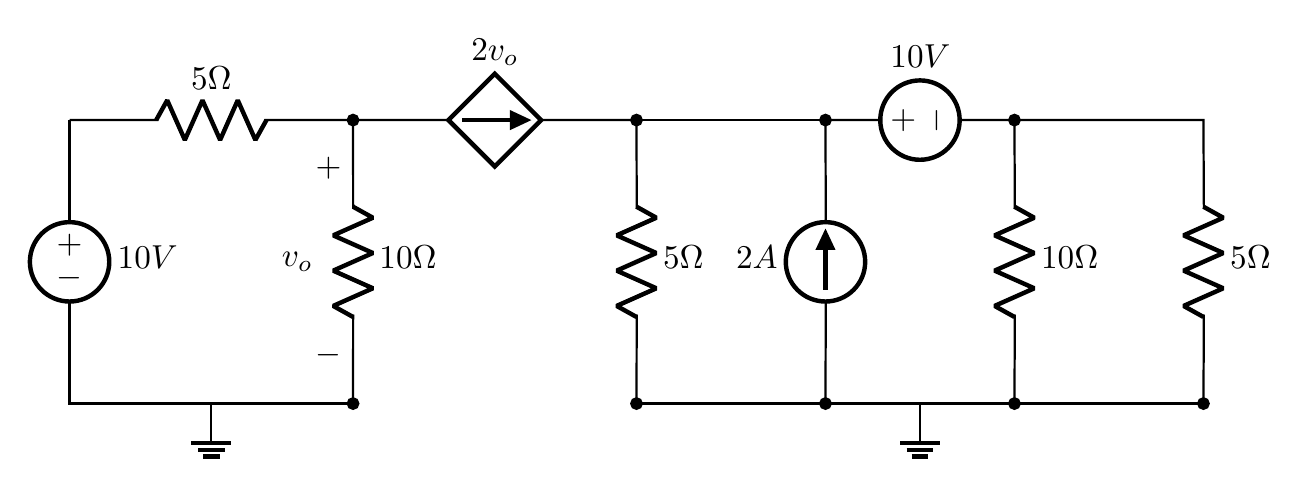
\begin{tikzpicture}[thick,american, scale=1.2, transform shape]

    % Left Sub-circuit
    % Drawn top to bottom for the voltage source to ensure '+' is at the top
    \draw (0,3) to[V, l=$10V$] (0,0) -- (3,0);
    \draw (0,3) to[R, l=$5\Omega$] (3,3) node[circ]{}
          to[R, l=$10\Omega$, v=$v_o$] (3,0) node[circ]{};
    \draw (1.5,0) node[ground]{};

    % Dependent Current Source connecting left and right circuits
    \draw (3,3) to[cI, l=$2v_o$] (6,3) node[circ]{};

    % Right Sub-circuit
    \draw (6,3) to[R, l=$5\Omega$] (6,0) node[circ]{};
    \draw (6,3) -- (8,3) node[circ]{};
    
    % Current source drawn from bottom to top so the arrow points up
    \draw (8,0) node[circ]{} to[I, l=$2A$] (8,3); 
    
    % Voltage source drawn left to right so '+' is on the left
    \draw (8,3) to[V, l=$10V$] (10,3) node[circ]{}; 
    
    \draw (10,3) to[R, l=$10\Omega$] (10,0) node[circ]{};
    \draw (10,3) -- (12,3) to[R, l=$5\Omega$] (12,0) node[circ]{};

    % Connect bottom nodes of the right sub-circuit to a common ground rail
    \draw (6,0) -- (12,0);
    \draw (9,0) node[ground]{};

\end{tikzpicture}
\end{center}
\mk{17} \yr{EEE 163 | L-1/T-1 | 2013--14}

\item Use KCL to obtain currents $i_1$, $i_2$ and $i_3$ in the circuit below.
\begin{center}
  \begin{tikzpicture}[american, scale=1.5]

    % Left branch
    % Current arrow pointing up
    \draw (0,0) to[short, i=$8mA$] (0,3);
    
    % Top branch
    \draw (0,3) -- (2.5,3);
    % Current arrow pointing right
    \draw (2.5,3) to[short, i=$12mA$] (5,3);
    
    % Right branch
    \draw (5,3) -- (5,0);
    
    % Middle upper branch
    % Current arrow pointing down
    \draw (2.5,3) to[short, i=$i_1$] (2.5,1.5);
    
    % Horizontal line for the inner split
    \draw (1.5,1.5) -- (3.5,1.5);
    
    % Inner left branch (i2)
    % Drawn from bottom to top so the arrow points up. 
    % i_ puts the label on the right side of the arrow, matching the image.
    \draw (1.5,0) to[short, i_=$i_2$] (1.5,1.5); 
    
    % Inner right branch (i3)
    % Drawn from top to bottom so the arrow points down.
    \draw (3.5,1.5) to[short, i=$i_3$] (3.5,0);
    
    % Bottom branch segments
    \draw (5,0) -- (3.5,0);
    % Current arrow pointing left (drawn right to left)
    \draw (3.5,0) to[short, i=$9mA$] (1.5,0);
    \draw (1.5,0) -- (0,0);

\end{tikzpicture}

\end{center}
\mk{9} \yr{EEE 163 | L-1/T-1 | 2013--14}

\item Using nodal analysis, find $v_1$ and $v_2$ in the circuit below.
\begin{center}
  \begin{circuitikz}[thick,scale=1.2, transform shape]
    % Bottom reference wire
    \draw (0,0) -- (8,0);
    
    % Leftmost branch: 5A independent current source pointing upwards
    \draw (0,0) to[I, l=5~A] (0,3) -- (2,3);
    
    % First vertical branch: 10 ohm resistor
    % (Path drawn bottom-to-top, l_ places label on the right)
    \draw (2,0) to[R, l_=10~$\Omega$] (2,3);
    
    % Top parallel branch: 5 ohm resistor
    \draw (2,3) -- (2,4.5) to[R, l=5~$\Omega$] (6,4.5) -- (6,3);
    
    % Middle horizontal branch: 8V independent voltage source 
    % (invert swaps polarity to put '-' on left and '+' on right, l_ puts label below)
    \draw (2,3) to[V, invert, l_=8~V] (6,3);
    
    % Second vertical branch: 5 ohm resistor
    % (Path drawn bottom-to-top, l places label on the left)
    \draw (6,0) to[R, l=5~$\Omega$] (6,3);
    
    % Rightmost branch: 2A independent current source pointing upwards
    % (Path drawn bottom-to-top, l_ places label on the right)
    \draw (8,0) to[I, l_=2~A] (8,3) -- (6,3);
    
    % Connection dots at main circuit junctions
    \node[circle, fill, inner sep=1.5pt] at (2,3) {};
    \node[circle, fill, inner sep=1.5pt] at (6,3) {};
    
    % Node labels (v1 and v2)
    \node[above left] at (2,3) {$v_1$};
    \node[above right] at (6,3) {$v_2$};
    
\end{circuitikz}

\end{center}
\mk{10} \yr{EEE 163 | L-1/T-1 | 2012--13}

\item Using nodal analysis, find the voltage drop $V$ across the 4\,$\Omega$ resistance for the circuit shown below.
\begin{center}
  \begin{circuitikz}[thick, american, scale=1.2, transform shape]

    % --- Bottom Ground Rail ---
    \draw (0,0) -- (7.5,0);

    % --- Leftmost Vertical Column ---
    % 15V Battery at the bottom half, 3 Ohm resistor at the top half
    \draw (0,0) to[battery2,invert,l_=$15\text{ V}$] (0,2.5)
                to[R, l_=$3\Omega$] (0,5);

    % --- Top Horizontal Rail to Triangle Apex ---
    \draw (0,5) -- (5,5);

     \draw (5,5) to[R, l=$7\Omega$, -*] (2.5,2.5);
    % Right diagonal
    \draw (5,5) to[R, l_=$7\Omega$, -*] (7.5,2.5);

    % --- Middle Horizontal Rail & Vertical Columns ---
    % Connection from Left Node to Center Node
    \draw (2.5,2.5) -- (5,2.5);
    
    % Vertical Column 1: 5 Ohm Resistor
    \draw (2.5,2.5) to[R, l_=$5\Omega$, *-*] (2.5,0);
    
    % Vertical Column 2: 3A Current Source (pointing DOWN)
    \draw (4.5,2.5) to[I, l=$3\text{ A}$, *-*] (4.5,0);
    
    % Connection from Center Node to Right Node containing:
    % 4 Ohm Resistor (with voltage drop V) and a 4V Battery
    \draw (5,2.5) to[R, l=$4\Omega$, v=$V$] (6.3,2.5)
                  to[battery2, l_=$4\text{ V}$] (7.5,2.5);
                    
    % Vertical Column 3: 6 Ohm Resistor
    \draw (7.5,2.5) to[R, l=$6\Omega$, *-*] (7.5,0);


\end{circuitikz}
\end{center}
\mk{18} \yr{EEE 163 | L-1/T-1 | 2010--11}

\item Using nodal analysis, calculate the power of the 25\,V voltage source in the circuit shown below.
\begin{center}
  \begin{circuitikz}[thick,american, scale=1.2, transform shape]
    % Main top and bottom horizontal rails
    \draw (0,6) -- (10.5,6);
    \draw (0,0) -- (8,0);

    % Leftmost branch (330k Resistor)
    \draw (0,6) to[R, l=$330\text{ k}\Omega$] (0,0);

    % Second branch (15V and 25V Independent Voltage Sources)
    \draw (2,0) to[V, l=$25\text{ V}$] (2,3);
    \draw (2,6) to[V, l_=$15\text{ V}$] (2,3);
                
    % Central horizontal branch with 560k resistor
    \draw (2,3) to[R, l=$560\text{ k}\Omega$, *-*] (5,3);
    
    % Ground connection along the center horizontal wire
    \draw (5,3) -- (6.5,3) node[ground] {};
    \draw (6.5,3) -- (8,3);

    % Third branch (Two 330k Resistors)
    \draw (5,6) to[R, l=$330\text{ k}\Omega$] (5,3);
    \draw (5,3) to[R, l=$330\text{ k}\Omega$] (5,0);

    % Rightmost vertical branches and sources
    % Top-right independent current source (0.13mA pointing up)
    \draw (8,3) to[I, l_=$0.13\text{ mA}$] (8,6);
    
    % Middle-right resistor (600k)
    \draw (8,3) to[R, l_=$600\text{ k}\Omega$, *-*] (8,1.5);
    
    % Bottom-right independent current source (0.5mA pointing up)
    \draw (8,0) to[I, l=$0.5\text{ mA}$] (8,1.5);

    % Far-right feedback/bypass wire loop
    \draw (8,1.5) -- (10.5,1.5) -- (10.5,6);

    % Explicit connection nodes for visual clarity
    \node[circ] at (0,6) {};
    \node[circ] at (0,0) {};
    \node[circ] at (2,6) {};
    \node[circ] at (2,0) {};
    \node[circ] at (5,6) {};
    \node[circ] at (5,0) {};
    \node[circ] at (8,6) {};
    \node[circ] at (8,0) {};
    \node[circ] at (8,3) {};


\end{circuitikz}
\end{center}
\mk{17} \yr{EEE 163 | L-1/T-1 | 2008--09}

\item Using Node Voltage Analysis method, find $v$ in the circuit shown below. (Reference ground for the circuit is indicated.)
\begin{center}
  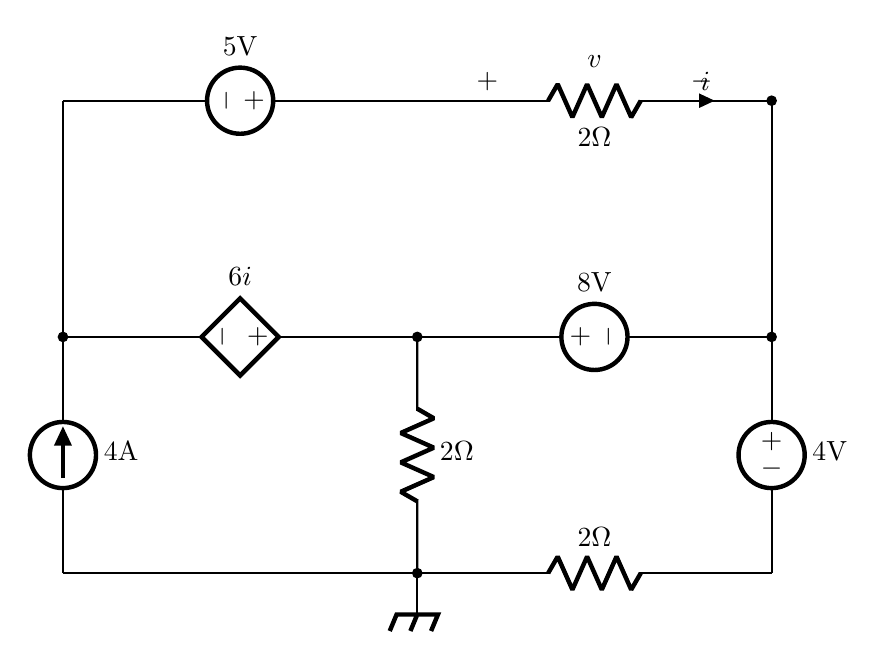
\begin{tikzpicture}[american, thick, x =1.5cm , y=1.5cm]

    % --- Left Branch ---
    % 4A Independent Current Source (Arrow UP)
    \draw (0,0) to[I, l_=$4\text{A}$] (0,2) -- (0,4);
    
    % --- Top Branch ---
    % 5V Voltage Source (- on left, + on right)
    \draw (0,4) to[V, invert, l=$5\text{V}$] (3,4);
    % 2 Ohm Resistor with voltage 'v' and current 'i'
    \draw (3,4) to[R, l_=$2\Omega$, v^=$v$, i>=$i$] (6,4);
    
    % --- Middle Horizontal Branch ---
    % 6i Dependent Voltage Source (- on left, + on right)
    \draw (0,2) to[cV, invert, l=$6i$] (3,2);
    % 8V Independent Voltage Source (+ on left, - on right)
    \draw (3,2) to[V, l=$8\text{V}$] (6,2);
    
    % --- Center Vertical Branch ---
    % 2 Ohm Resistor
    \draw (3,2) to[R, l=$2\Omega$] (3,0);
    
    % --- Right Vertical Branch ---
    \draw (6,4) -- (6,2);
    % 4V Voltage Source (+ on top, - on bottom)
    \draw (6,2) to[V, l=$4\text{V}$] (6,0);
    
    % --- Bottom Branch ---
    \draw (0,0) -- (3,0);
    % 2 Ohm Resistor
    \draw (3,0) to[R, l=$2\Omega$] (6,0);
    
    % --- Ground ---
    % Chassis ground symbol at the center bottom node
    \node[cground] at (3,0) {};
    
    % --- Junction Dots ---
    \filldraw (0,2) circle (1.5pt);
    \filldraw (3,2) circle (1.5pt);
    \filldraw (6,2) circle (1.5pt);
    \filldraw (3,0) circle (1.5pt);
    \filldraw (6,4) circle (1.5pt);
    

\end{tikzpicture}
\end{center}
\mk{16} \yr{EEE 163 | L-1/T-1 | 2007--08}

\item Find the voltages at nodes a, b, c, d \& e using Node Voltage Analysis for the circuit shown below.
\begin{center}
  \begin{circuitikz}[thick]

    % ---------------------------------------------------
    % Central Axis & Current Source
    % ---------------------------------------------------
    % From top node 'a' to central intersection (0,0)
    \draw (0,2.5) -- (0,0);
    % 2A Current source pointing up from node 'e' to central intersection
    \draw (0,-2) to[I, l=$2\text{A}$] (0,0);

    % ---------------------------------------------------
    % Horizontal Middle Branches
    % ---------------------------------------------------
    \draw (-3,0) to[R, l=$150\,\Omega$] (0,0);
    \draw (0,0) to[R, l=$100\,\Omega$] (3,0);

    % ---------------------------------------------------
    % Top Slanted Roof Branches
    % ---------------------------------------------------
    \draw (0,2.5) to[R, l_=$150\,\Omega$] (-3,0);
    \draw (0,2.5) to[R, l=$100\,\Omega$] (3,0);

    % ---------------------------------------------------
    % Lower Outer Branches
    % ---------------------------------------------------
    \draw (-3,0) to[R, l_=$25\,\Omega$] (-2.5,-3.5);
    \draw (3,0) to[R, l=$50\,\Omega$] (2.5,-3.5);

    % ---------------------------------------------------
    % Bottom Outer Wire
    % ---------------------------------------------------
    \draw (-2.5,-3.5) -- (2.5,-3.5);

    % ---------------------------------------------------
    % Lower Inner Branches to Node e
    % ---------------------------------------------------
    \draw (-2.5,-3.5) to[R, l=$20\,\Omega$] (0,-2);
    \draw (2.5,-3.5) to[R, l_=$20\,\Omega$] (0,-2);

    % ---------------------------------------------------
    % Node Labels
    % ---------------------------------------------------
    \node[above] at (0,2.5) {$a$};
    \node[left] at (-3,0) {$b$};
    \node[right] at (3,0) {$c$};
    \node[left] at (-2.5,-3.5) {$d$};
    \node[below] at (0,-2.1) {$e$};


\end{circuitikz}
\end{center}
\mk{20} \yr{EEE 163 | L-1/T-1 | 2006--07}

\item For the circuit shown below, find $V_1$, $V_2$ and $V_3$ using nodal analysis.
\begin{center}
  
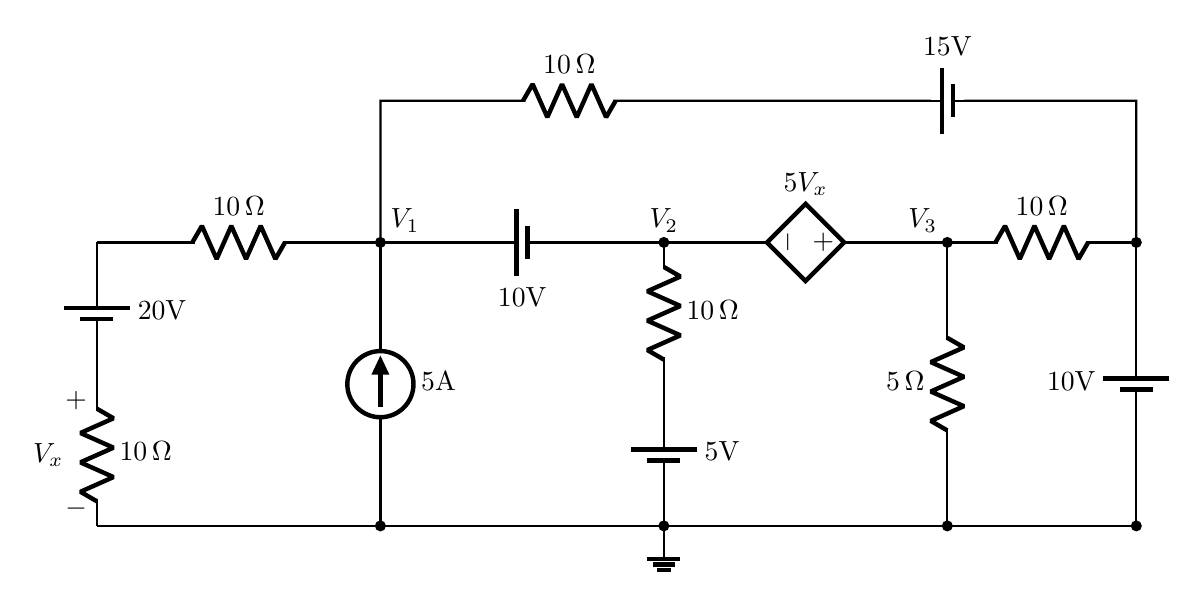
\begin{tikzpicture}[thick, x=1.2cm, y=1.2cm, >=stealth]

    % --- Bottom Ground Wire ---
    \draw (0,0) -- (11,0);
    \node[ground] at (6,0) {};

    % --- Far Left Branch ---
    % Drawn top-to-bottom for correct V_x polarity (+ at top, - at bottom) and label placements.
    \draw (0,1.5) to[R, l=$10\,\Omega$, v=$V_x$] (0,0);
    % 20V Battery drawn bottom-to-top to keep long plate (positive) at the top.
    \draw (0,3) to[battery1, l=$20\text{V}$] (0,1.5);
    % Top-left horizontal wire
    \draw (0,3) to[R, l=$10\,\Omega$] (3,3);

    % --- V1 Branch (x=3) ---
    % 5A independent current source, arrow pointing UP
    \draw (3,0) to[I, l_=$5\text{A}$] (3,3);

    % --- V1 to V2 Branch (x=3 to 6) ---
    % 10V battery with long plate on the left. Drawn right-to-left.
    \draw (3,3) to[battery1, l_=$10\text{V}$] (6,3);

    % --- V2 Branch (x=6) ---
    % 5V battery (long plate top) and 10 Ohm resistor. Drawn bottom-to-top.
    \draw (6,0) to[battery1, invert,l_=$5\text{V}$] (6,1.5) to[R, l_=$10\,\Omega$] (6,3);

    % --- V2 to V3 Branch (x=6 to 9) ---
    % Dependent voltage source 5V_x with + on the right. Drawn right-to-left.
    \draw (9,3) to[cV, l_=$5V_x$] (6,3);

    % --- V3 Branch (x=9) ---
    % 5 Ohm resistor. Drawn top-to-bottom.
    \draw (9,3) to[R, l_=$5\,\Omega$] (9,0);

    % --- V3 to Rightmost Branch (x=9 to 11) ---
    \draw (9,3) to[R, l=$10\,\Omega$] (11,3);

    % --- Rightmost Vertical Branch (x=11) ---
    % 10V battery with long plate on top. Drawn bottom-to-top.
    \draw (11,3) to[battery1, l_=$10\text{V}$] (11,0);

    % --- Topmost Branch (Parallel from V1 to far right) ---
    \draw (3,3) -- (3,4.5) to[R, l=$10\,\Omega$] (7,4.5) to[battery1, l=$15\text{V}$] (11,4.5) -- (11,3);

    % --- Node Labels and Explicit Junction Dots ---
    \node[above right] at (3,3) {$V_1$};
    \node[above] at (6,3) {$V_2$};
    \node[above left] at (9,3) {$V_3$};

    \fill (3,3) circle (2pt);
    \fill (6,3) circle (2pt);
    \fill (9,3) circle (2pt);
    \fill (11,3) circle (2pt);
    
    \fill (3,0) circle (2pt);
    \fill (6,0) circle (2pt);
    \fill (9,0) circle (2pt);
    \fill (11,0) circle (2pt);

\end{tikzpicture}
\end{center}
\mk{17} \yr{EEE 163 | L-1/T-1 | 2005--06}

\end{enumerate}

%%──────────────────────────────────────────────────────────────────────
\subtopic{cA}{Network Theorems (Superposition, Th\'{e}venin, Norton, MPT)}
\label{sub:s1-theorems}

\begin{enumerate}

\item The variable resistor $R_o$ in the circuit shown below is adjusted so that 
maximum power is transferred to $R_o$. Find the maximum power delivered to this resistor. 
How much power does the $280 \text{ V}$ source deliver to the circuit in this condition?  

\begin{center}
  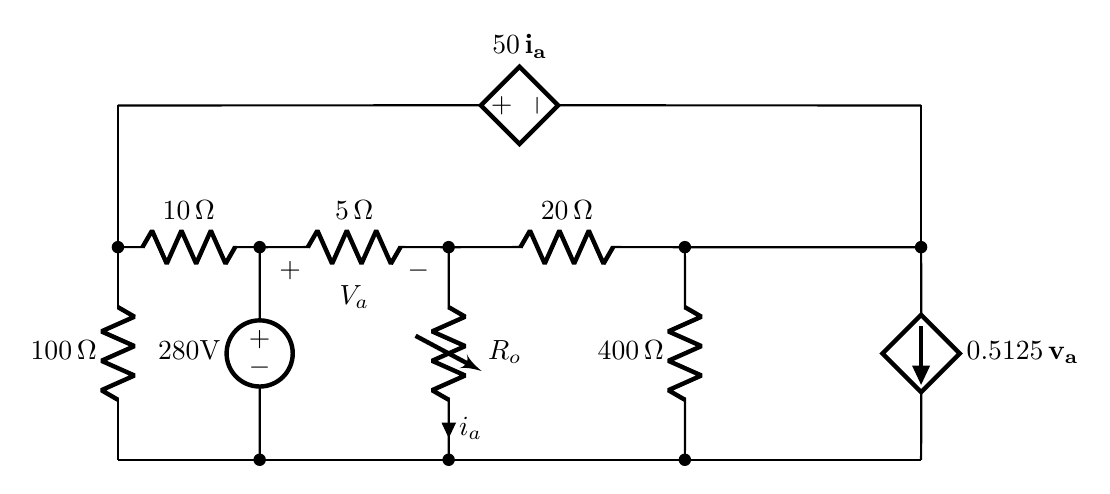
\begin{tikzpicture}[thick, scale=1.5]

    % --- BASE GRID GROUND RAIL ---
    \draw (0,0) -- (6.8,0);

    % --- LEFTMOST COMPONENT ---
    % 100 ohm vertical resistor
    \draw (0,0) to[R, l=$100\,\Omega$] (0,1.8);

    % --- FIRST INTERMEDIATE VERTICAL BRANCH ---
    % 280V Independent DC Voltage Source
    \draw (1.2,1.8) to[V, l_=$280\text{V}$] (1.2,0);

    % --- MIDDLE VARIABLE LOAD BRANCH ---
    % Variable resistor Ro with current arrow ia pointing down
    \draw (2.8,1.8) to[variable resistor, l=$R_o$, i>=$i_a$] (2.8,0);

    % --- RIGHT INTERMEDIATE VERTICAL BRANCH ---
    % 400 ohm vertical resistor
    \draw (4.8,0) to[R, l=$400\,\Omega$] (4.8,1.8);

    % --- RIGHTMOST DEPENDENT BRANCH ---
    % 0.5125*va Dependent Current Source (pointing down)
    \draw (6.8,1.8) to[cI, l=$0.5125\,\mathbf{v_a}$] (6.8,0);

    % --- MIDDLE ROW HORIZONTAL CONNECTIONS & RESISTOR CORES ---
    \draw (0,1.8) to[R, l=$10\,\Omega$] (1.2,1.8)
                  to[R, l=$5\,\Omega$, v=$V_a$] (2.8,1.8)
                  to[R, l=$20\,\Omega$] (4.8,1.8)
                  -- (6.8,1.8);

    % --- OVERHEAD PARALLEL BRIDGE ---
    % Vertical extensions for the top loop
    \draw (0,1.8) -- (0,3);
    \draw (6.8,1.8) -- (6.8,3);
    
    % Topmost horizontal line containing the 50*ia Dependent Voltage Source
    \draw (0,3) to[cvsource, l=$50\,\mathbf{i_a}$] (6.8,3);

    % --- JUNCTION DOTS ---
    % Top bridge corner split-points
    \fill (0,1.8) circle (1.5pt);
    \fill (6.8,1.8) circle (1.5pt);
    % Main line junctions
    \fill (1.2,1.8) circle (1.5pt);
    \fill (2.8,1.8) circle (1.5pt);
    \fill (4.8,1.8) circle (1.5pt);
    % Bottom line junctions
    \fill (1.2,0) circle (1.5pt);
    \fill (2.8,0) circle (1.5pt);
    \fill (4.8,0) circle (1.5pt);

\end{tikzpicture}

\end{center}

\mk{20} \yr{EEE 163 | L-1/T-1 | 2024--25}


\item For the circuit shown below, if a 20\Omega resistor is connected between terminal a and b, find the current through it with the help of Thevenin\'s theorem.

\begin{center}
  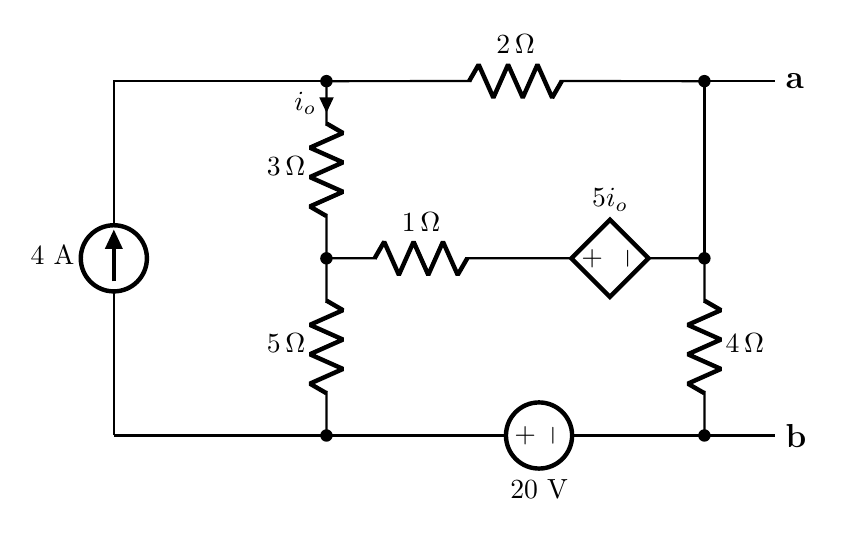
\begin{tikzpicture}[thick, scale=1.5]

    % --- MAIN NODES & GRID COORDINATES ---
    % Bottom line: Left=0, Middle=2, Right=5
    % Middle line: Height=1.5
    % Top line: Height=3

    % --- LEFTMOST VERTICAL BRANCH ---
    % 4A Independent Current Source (pointing up)
    \draw (0,0) to[I, l=$4\text{ A}$] (0,3) -- (1.8,3);

    % --- CENTER VERTICAL BRANCH STACK ---
    % Top-center resistor (3 ohm) with current arrow io pointing down
    \draw (1.8,3) to[R, l_=$3\,\Omega$, i>_=$i_o$] (1.8,1.5);
    % Bottom-center resistor (5 ohm)
    \draw (1.8,1.5) to[R, l_=$5\,\Omega$] (1.8,0);

    % --- HORIZONTAL MIDDLE BRIDGE ---
    % 1 ohm resistor connected in series with the 5_io dependent voltage source
    \draw (1.8,1.5) to[R, l=$1\,\Omega$] (3.4,1.5)
                    to[cvsource, l=$5i_o$] (5,1.5);

    % --- TOP HORIZONTAL BRANCH ---
    % 2 ohm resistor
    \draw (1.8,3) to[R, l=$2\,\Omega$] (5,3);

    % --- RIGHTMOST VERTICAL BRANCH STACK ---
    % Upper half connecting down to the bridge junction
    \draw (5,3) -- (5,1.5);
    % Lower half containing the 4 ohm resistor
    \draw (5,1.5) to[R, l=$4\,\Omega$] (5,0);

    % --- BOTTOM HORIZONTAL BRANCH ---
    % Left side line up to the 20V DC Source
    \draw (0,0) -- (1.8,0) -- (3,0);
    % 20V Independent Voltage Source
    \draw (3,0) to[V, l_=$20\text{ V}$] (4.2,0);
    % Right side line from source to the corner
    \draw (4.2,0) -- (5,0);

    % --- OUTPUT TERMINALS ---
    % Extended wire ports for terminals 'a' and 'b'
    \draw (5,3) -- (5.6,3) node[anchor=west, font=\large\bfseries] {a};
    \draw (5,0) -- (5.6,0) node[anchor=west, font=\large\bfseries] {b};

    % --- JUNCTION DOTS ---
    \fill (1.8,3) circle (1.5pt);
    \fill (1.8,1.5) circle (1.5pt);
    \fill (1.8,0) circle (1.5pt);
    \fill (5,3) circle (1.5pt);
    \fill (5,1.5) circle (1.5pt);
    \fill (5,0) circle (1.5pt);

\end{tikzpicture}

\end{center}


\mk{15} \yr{EEE 163 | L-1/T-1 | 2024--25}  

\item Find the current in the 10\,k$\Omega$ resistor ($i_o$) and the power developed by the 100V source making a succession of appropriate source transformations for the circuit below.
\begin{center}
  \begin{circuitikz}[thick, scale=1.2]
    % --- Far Left Loop ---
    % 100V Voltage Source (drawn top-to-bottom to match - on top, + on bottom)
    \draw (0,0) to[V, l_=$100\,\text{V}$] (0,3);
    
    % Top 20 kOhm resistor & first vertical 80 kOhm branch
    \draw (0,3) to[R, l=$20\,\text{k}\Omega$] (2.5,3)
          to[R, l=$80\,\text{k}\Omega$, *-*] (2.5,0)
          -- (0,0);
          
    % --- Middle Section ---
    % Top 3 kOhm, Current Source, and Bottom 1 kOhm resistor
    \draw (2.5,3) to[R, l=$3\,\text{k}\Omega$] (5.5,3)
          to[I, invert, l=$12\,\text{mA}$, *-*] (5.5,0)
          to[R, l=$1\,\text{k}\Omega$] (2.5,0);
          
    % --- Parallel 60 kOhm Branch ---
    \draw (5.5,3) -- (7.5,3)
          to[R, l=$60\,\text{k}\Omega$, *-*] (7.5,0)
          -- (5.5,0);
          
    % --- Rightmost Section & Output Load ---
    % Top 5 kOhm resistor leading to the terminal node dot
    \draw (7.5,3) to[R, l=$5\,\text{k}\Omega$] (10,3) node[circle, fill, inner sep=1.5pt] {};
    \draw (7.5,0) -- (10,0) node[circle, fill, inner sep=1.5pt] {};
    
    % Final 10 kOhm load branch with downward current arrow i_o
    \draw (10,3) -- (11.5,3)
          to[R, l=$10\,\text{k}\Omega$, i=$i_o$] (11.5,0)
          -- (10,0);
          
\end{circuitikz}

\end{center}
\mk{15/12} \yr{EEE 163 | L-1/T-1 | 2024--25, 2017--18}

  
\item For the circuit shown below,
use superposition principle to find magnitude and nature of the power associated with the 50\,$\Omega$ resistor.

\begin{center}
  
\begin{circuitikz}[thick ,american, x=0.9cm,transform shape]

    % Left branch: 100V Voltage Source
    \draw (0,6) to[V, l=$100\text{ V}$] (0,0);

    % Top horizontal branch (left part): 50 Ohm Resistor
    \draw (0,6) to[R, l=$50\ \Omega$] (4,6);

    % Middle vertical branch 1: 10 Ohm Resistor
    % l_ places the label on the left side of the vertical wire
    \draw (4,6) to[R, l_=$10\ \Omega$] (4,3);
    
    % Manually drawing the i_o current arrow to match the exact position in the image
    \draw[-latex] (3.3, 5.5) -- (3.3, 4.5) node[midway, left] {$i_o$};

    % Top horizontal branch (right part): 10 Ohm Resistor with v_o voltage label
    % v_ places the voltage polarity and label below the resistor
    \draw (4,6) to[R, l=$10\ \Omega$, v_=$v_o$] (8,6);

    % Middle vertical branch 2: Dependent Voltage Source
    \draw (8,6) to[cV, l=$4i_o$] (8,3);

    % Far right vertical branch: 40 Ohm Resistor
    \draw (8,6) -- (11,6) to[R, l=$40\ \Omega$] (11,0);

    % Middle horizontal connecting wire
    \draw (4,3) -- (8,3);

    % Bottom vertical branch 1: Dependent Current Source
    % Drawn top-to-bottom so the arrow points down
    \draw (4,3) to[cI, l_=$0.2v_o$] (4,0);

    % Bottom vertical branch 2: Independent Current Source
    % Drawn bottom-to-top so the arrow points up
    \draw (8,0) to[I, l_=$2\text{ A}$] (8,3);

    % Bottom return wire connecting all branches
    \draw (0,0) -- (11,0);

\end{circuitikz}
\end{center}
  \mk{20} \yr{EEE 163 | L-1/T-1 | 2024--25}

\item For the circuit shown below, if a 5\,$\Omega$ resistor is connected between terminals a and b, find the current through it with the help of Th\'{e}venin's theorem. 
\begin{center}
  \begin{circuitikz}[thick , american, scale=1.2, transform shape]

    % Bottom wire with connection nodes and terminal 'b'
    \draw (0,0) -- (2,0) node[circ]{} 
          -- (6.5,0) node[circ]{} 
          -- (8.5,0) node[circ]{} 
          -- (10.5,0) node[circ]{} node[right]{b};

    % Leftmost parallel branches
    \draw (0,0) to[R, l=$60\ \Omega$] (0,3) -- (2,3) node[circ]{};
    \draw (2,0) to[I, l=$4\text{ A}$] (2,3);

    % Top horizontal branch with 20 Ohm resistor and Dependent Voltage Source
    % 'invert' ensures the + sign is on the left and - is on the right
    \draw (2,3) to[R, l=$20\ \Omega$] (4.5,3);
    \draw (6.5,3) to[cV, invert, l=$160\ i_\Delta$, -*] (4.5,3);

    % 80 Ohm vertical resistor
    \draw (6.5,3) to[R, l=$80\ \Omega$] (6.5,0);

    % Connection to the 40 Ohm resistor
    \draw (6.5,3) to[short, -*] (8.5,3);

    % 40 Ohm vertical resistor with current i_\Delta pointing downwards
    \draw (8.5,3) to[R, l=$40\ \Omega$, i=$i_\Delta$] (8.5,0);

    % Top right wire leading to terminal 'a'
    \draw (8.5,3) -- (10.5,3) node[circ]{} node[right]{a};

\end{circuitikz}
\end{center}
\mk{20} \yr{EEE 163 | L-1/T-1 | 2023--24}

\item For the circuit shown below, use the superposition principle to calculate the power dissipated by the 5\,$\Omega$ resistor. [The circuit contains resistors: 3\,$\Omega$, 2\,$\Omega$, 1\,$\Omega$, 5\,$\Omega$, 4\,$\Omega$; Sources: 4\,A independent current source, $5i_o$ dependent voltage source, 20\,V independent voltage source.]
\begin{center}
  \begin{circuitikz}[thick, american, scale=1.2, transform shape]

    % Left vertical branch: 4A Independent Current Source (pointing up)
    \draw (0,0) to[I, l=$4\text{ A}$] (0,4) -- (3,4);

    % Top horizontal branch: 2 Ohm Resistor
    \draw (3,4) to[R, l=$2\ \Omega$] (7,4) -- (7,2);

    % Middle vertical branch - Upper part: 3 Ohm Resistor
    \draw (3,4) to[R, l=$3\ \Omega$, *-*] (3,2);
    
    % Middle vertical branch - Lower part: 5 Ohm Resistor with current i_o pointing down
    \draw (3,2) to[R, l=$5\ \Omega$, i=$i_o$, -*] (3,0);

    % Center horizontal branch: 1 Ohm Resistor and Dependent Voltage Source (5i_o)
    % Drawn left-to-right so + is on the left and - is on the right
    \draw (3,2) to[R, l=$1\ \Omega$] (5.2,2)
          to[cV, l=$5i_o$, -*] (7,2);

    % Right vertical branch: 4 Ohm Resistor
    \draw (7,2) to[R, l=$4\ \Omega$] (7,0);

    % Bottom horizontal branch: wire and 20V Independent Voltage Source
    % Drawn left-to-right so + is on the left and - is on the right
    \draw (0,0) -- (3,0) to[V, l=$20\text{ V}$] (7,0);

\end{circuitikz}
\end{center}
\mk{15} \yr{EEE 163 | L-1/T-1 | 2023--24}

\item Obtain the Norton equivalent circuit at terminals a--b of the network shown below.
\begin{center}
  
\begin{circuitikz}[thick, american, scale=1.2, transform shape]

    % ==========================================
    % 1. Left Loop (50V Source and 3 Ohm Resistor)
    % ==========================================
    % Voltage source pointing upwards
    \draw (0,3) to[V, l=$50\text{ V}$] (0,0);
               \draw (0,3) to[R, l=$3\ \Omega$] (3,3);

    % ==========================================
    % 2. Middle Branches (6 Ohm and Dependent Source)
    % ==========================================
    % 6 Ohm Resistor with voltage Vx
    % 'v_=' places the Vx label on the right with + on top, - on bottom
    \draw (3,3) to[R, l=$6\ \Omega$, v_=$v_x$] (3,0);
    
    % Top connecting wire with 2 Ohm Resistor
    \draw (3,3) to[R, l=$2\ \Omega$] (6,3);
    
    % Dependent Current Source pointing upwards
    \draw (6,0) to[cI, l=$0.5 v_x$] (6,3);

    % ==========================================
    % 3. Right Branch (10 Ohm Resistor and Terminals)
    % ==========================================
    % Top wire extending to the 10 Ohm resistor
    \draw (6,3) -- (8,3) to[R, l=$10\ \Omega$] (8,0);
    
    % Open terminals a and b
    \draw (8,3) -- (9.5,3) node[ocirc] {} node[right] {$a$};
    \draw (8,0) -- (9.5,0) node[ocirc] {} node[right] {$b$};

    % ==========================================
    % 4. Bottom Common Wire and Junction Dots
    % ==========================================
    % Connecting all bottom nodes to the negative terminal
    \draw (0,0) -- (8,0);
    
    % Adding connection dots (circ) where 3 or more wires meet
    \node[circ] at (3,3) {};
    \node[circ] at (3,0) {};
    \node[circ] at (6,3) {};
    \node[circ] at (6,0) {};
    \node[circ] at (8,3) {};
    \node[circ] at (8,0) {};

\end{circuitikz}
\end{center}
\mk{17} \yr{EEE 163 | L-1/T-1 | 2022--23}

\item For the circuit shown below, use the superposition principle to calculate the power dissipated by the 4\,$\Omega$ resistor.
\begin{center}
  
\begin{circuitikz}[thick , american, scale=1.2, transform shape]

    % ==========================================
    % 1. Left Loop (10V Source and 2 Ohm Resistor)
    % ==========================================
    % 10V Voltage source pointing upwards (+ on top)
    \draw (0,3) to[V, l=$10\text{ V}$] (0,0);
                % 2 Ohm resistor connecting to the middle junction
               \draw (0,3) to[R, l=$2\ \Omega$] (3,3);

    % ==========================================
    % 2. Middle Branch (2A Current Source)
    % ==========================================
    % 2A Current source pointing upwards
    \draw (3,0) to[I, l=$2\text{ A}$] (3,3);

    % ==========================================
    % 3. Right Section (Dependent Source & Resistors)
    % ==========================================
    % Dependent Current Source (0.5 Vo) connecting middle to right
    \draw (3,3) to[cI, l=$0.5 V_o$] (6,3);
    
    % 1 Ohm Resistor in parallel with the dependent source
    \draw (3,3) -- (3,4.5) 
                to[R, l=$1\ \Omega$] (6,4.5) 
                -- (6,3);

    % 4 Ohm Resistor on the rightmost branch with Voltage Vo
    % 'l_=' places 4 Ohm on the left, 'v^=' places Vo on the right with + on top
    \draw (6,3) to[R, l_=$4\ \Omega$, v^=$V_o$] (6,0);

    % ==========================================
    % 4. Bottom Common Wire and Junction Dots
    % ==========================================
    % Connecting all bottom nodes
    \draw (0,0) -- (6,0);
    
    % Adding connection dots (circ) where 3 or more wires meet
    \node[circ] at (3,3) {};
    \node[circ] at (3,0) {};
    \node[circ] at (6,3) {};
    \node[circ] at (6,0) {};


\end{circuitikz}
\end{center}
\mk{18} \yr{EEE 163 | L-1/T-1 | 2022--23}

\item For the circuit below, if a 5\,$\Omega$ resistor is connected between terminals a and b, find the current through it with the help of Th\'{e}venin's theorem.
\begin{center}
  
\begin{circuitikz}[thick , american, scale=1.2, transform shape]

    % ==========================================
    % 1. Left Outer Branch
    % ==========================================
    % 2 Ohm Resistor and 12V Source (+ on top)
    \draw (0,2.5) to[R, l=$2\ \Omega$] (0,0);
               \draw (0, 5) to[V, l=$12\text{ V}$] (0,2.5);

    % ==========================================
    % 2. Right Outer Branch
    % ==========================================
    % 2 Ohm Resistor and 12V Source (+ on top)
    % 'l_=' places the labels on the right side
    \draw (8,2.5) to[R, l_=$2\ \Omega$] (8,0);
               \draw (8, 5) to[V, l_=$12\text{ V}$] (8,2.5);

    % ==========================================
    % 3. Top Wire & Inner Pi-Network (Upper part)
    % ==========================================
    % Connecting left branch to the Pi-network
    \draw (0,5) -- (2.5,5);
    
    % Top 2 Ohm Resistor
    \draw (2.5,5) to[R, l=$2\ \Omega$] (5.5,5);
    
    % Connecting Pi-network to the right branch
    \draw (5.5,5) -- (8,5);

    % Inner Vertical 6 Ohm Resistors
    % Drawn from bottom to top to easily place labels on left/right
    \draw (2.5,2.5) to[R, l=$6\ \Omega$] (2.5,5);
    \draw (5.5,2.5) to[R, l_=$6\ \Omega$] (5.5,5);

    % Middle Horizontal Wire joining the two 6 Ohm resistors
    \draw (2.5,2.5) -- (5.5,2.5);

    % ==========================================
    % 4. Middle Vertical Branch
    % ==========================================
    % Contains a 12V source (- on top, + on bottom) and a 6 Ohm resistor
    % 'invert' flips the polarity so + is at the bottom (start point)
    \draw (4,1.5) to[V, invert, l_=$12\text{ V}$] (4,0);
              \draw (4, 1.5)  to[R, l_=$6\ \Omega$] (4,2.5);

    % ==========================================
    % 5. Bottom Common Wire and Terminals
    % ==========================================
    % Bottom common ground wire connected to terminal b
    \draw (0,0) -- (9.5,0) node[ocirc] {} node[right] {$b$};
    
    % Top wire extending to terminal a
    \draw (8,5) -- (9.5,5) node[ocirc] {} node[right] {$a$};

    % Adding connection dots (circ) where 3 wires meet
    \node[circ] at (2.5,5) {};
    \node[circ] at (5.5,5) {};
    \node[circ] at (4,2.5) {};
    \node[circ] at (4,0) {};
    \node[circ] at (8,5) {};
    \node[circ] at (8,0) {};

  

\end{circuitikz}
\end{center}
\mk{18} \yr{EEE 163 | L-1/T-1 | 2022--23}

\item Obtain the Norton equivalent circuit at terminals a--b of the network as shown below.
\begin{center}
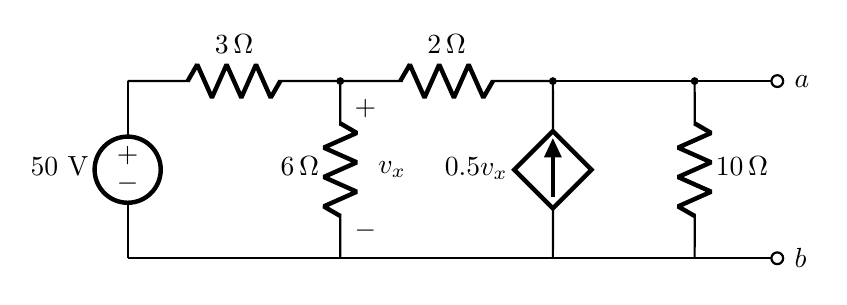
\begin{tikzpicture}[thick, scale=1.5]

    % Bottom wire line connection
    \draw (0,0) -- (5.5,0);

    % Leftmost DC Voltage Source branch
    \draw (0,0) to[V, invert, l=$50\text{ V}$] (0,1.5);

    % Top horizontal branch: 3 ohm and 2 ohm resistors in series
    \draw (0,1.5) to[R, l=$3\,\Omega$] (1.8,1.5) node[circle, fill, inner sep=1pt] (n1) {}
                  to[R, l=$2\,\Omega$] (3.6,1.5) node[circle, fill, inner sep=1pt] (n2) {};
                  
    % Vertical 6 ohm resistor with dependent voltage label vx
    \draw (1.8,1.5) to[R, l_=$6\,\Omega$, v^=$v_x$] (1.8,0);

    % Dependent Current Source branch (pointing up)
    \draw (3.6,0) to[cisource, l=$0.5v_x$] (3.6,1.5);

    % Connecting line from middle junction to the right section
    \draw (3.6,1.5) -- (4.8,1.5) node[circle, fill, inner sep=1pt] (n3) {};

    % Vertical 10 ohm Resistor
    \draw (4.8,1.5) to[R, l=$10\,\Omega$] (4.8,0);

    % Extensions to the open output terminals a and b
    \draw (4.8,1.5) -- (5.5,1.5) node[circle, draw, fill=white, inner sep=1.5pt, label=right:$a$] {};
    \draw (4.8,0)   -- (5.5,0)   node[circle, draw, fill=white, inner sep=1.5pt, label=right:$b$] {};

\end{tikzpicture}

\end{center}
\mk{23} \yr{EEE 163 | L-1/T-1 | 2021--22}


\item For the circuit shown below, use the superposition principle to find the current $i$ and thereby calculate the power dissipated in the 3\,$\Omega$ resistor.
\begin{center}
  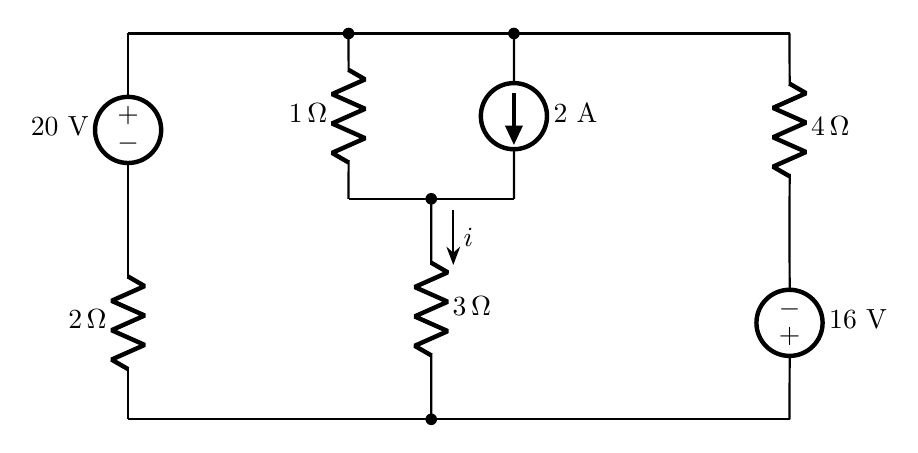
\begin{tikzpicture}[thick, american, scale=1.4]
    
    % Bottom reference rail
    \draw (0,0) -- (6,0);
    
    % Top rail
    \draw (0,3.5) -- (6,3.5);
    
    % Leftmost branch: 20V independent voltage source + 2 ohm resistor
    \draw (0,0) to[R, l=$2\,\Omega$] (0,1.75)
                to[V, invert, l=$20\text{ V}$] (0,3.5);
                
    % Central upper parallel structure (1 ohm resistor and 2A current source)
    \draw (2,3.5) to[R, l_=$1\,\Omega$] (2,2);
    \draw (3.5,3.5) to[I, l=$2\text{ A}$] (3.5,2);
    
    % Horizontal wire tying the bottom of the 1 ohm resistor and 2A source together
    \draw (2,2) -- (3.5,2);
    
    % Central lower branch: 3 ohm resistor branching from the middle of the tie-wire
    \draw (2.75,2) to[R, l=$3\,\Omega$] (2.75,0);
    
    % Current label 'i' flowing into the 3 ohm resistor
    \draw[-{Stealth}, thick] (2.95,1.9) -- (2.95,1.4) node[midway, right] {$i$};
    
    % Rightmost branch: 4 ohm resistor + 16V independent voltage source (note inverted polarity)
    \draw (6,3.5) to[R, l=$4\,\Omega$] (6,1.75)
                to[V, l=$16\text{ V}$, invert] (6,0);

    % Explicit junction connection dots
    \fill (2,3.5) circle (1.5pt);
    \fill (3.5,3.5) circle (1.5pt);
    \fill (2.75,2) circle (1.5pt);
    \fill (2.75,0) circle (1.5pt);

\end{tikzpicture}

\end{center}
\mk{20/25} \yr{EEE 163 | L-1/T-1 | 2021--22, 2020--21}


\item For the circuit below, determine the value of $R_L$ that will draw the maximum power from the rest of the circuit and calculate the maximum power.
\begin{center}
  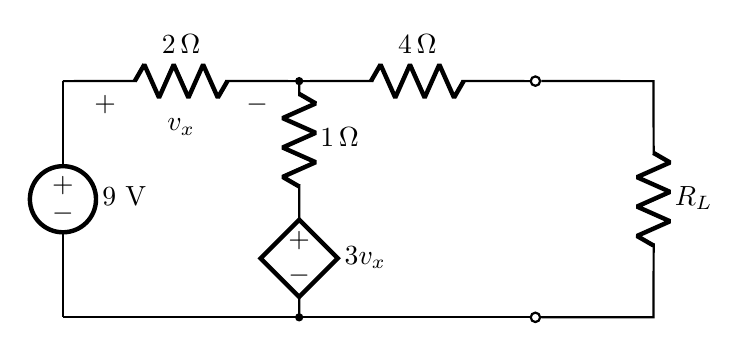
\begin{tikzpicture}[thick, scale=1.5]

    % Bottom wire line connection
    \draw (0,0) -- (5,0);

    % Leftmost branch: 9V DC Voltage Source
    \draw (0,2) to[V, l=$9\text{ V}$] (0,0);

    % Top horizontal branch: 2 ohm resistor with voltage drop vx
    \draw (0,2) to[R, l=$2\,\Omega$, v_=$v_x$] (2,2);
    
    % Continuing top horizontal path to the 4 ohm resistor
    \draw (2,2) to[R, l=$4\,\Omega$] (4,2);

    % Center vertical branch: 1 ohm resistor in series with a dependent voltage source
    \draw (2,2) to[R, l=$1\,\Omega$] (2,1)
                to[cvsource, l=$3v_x$] (2,0);

    % Output terminals (open circles) before the load resistor RL
    \draw (4,2) node[circle, draw, fill=white, inner sep=1.2pt] (t1) {};
    \draw (4,0) node[circle, draw, fill=white, inner sep=1.2pt] (t2) {};

    % Rightmost branch: Load Resistor RL
    \draw (t1) -- (5,2)
               to[R, l=$R_L$] (5,0)
               -- (t2);

    % Standard T-junction dots for clarity
    \fill (2,2) circle (1pt);
    \fill (2,0) circle (1pt);

\end{tikzpicture}

\end{center}
\mk{15} \yr{EEE 163 | L-1/T-1 | 2021--22}


\item Using source transformation, find the value of $i_x$ and thereby compute the power dissipated in the 15\,$\Omega$ resistor for the circuit shown below.
\begin{center}
  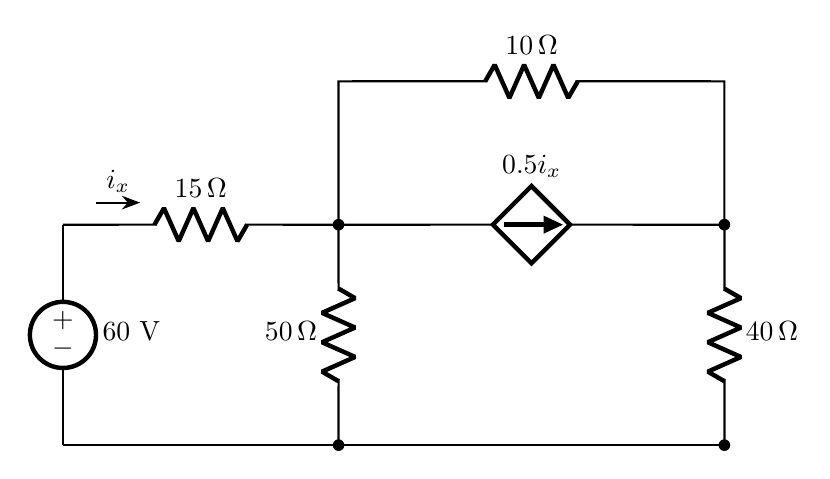
\begin{tikzpicture}[thick, american, scale=1.4]
    
    % Bottom reference rail
    \draw (0,0) -- (6,0);
    
    % Left branch: 60V independent DC voltage source
    \draw (0,2) to[V, l=$60\text{ V}$] (0,0);
    
    % Series resistor branch from source with current ix indicator
    \draw (0,2) to[R, l=$15\,\Omega$] (2.5,2);
    \draw[-{Stealth}, thick] (0.3,2.2) -- (0.7,2.2) node[midway, above] {$i_x$};
    
    % First vertical parallel resistor (50 ohm)
    \draw (2.5,2) to[R, l_=$50\,\Omega$] (2.5,0);
    
    % Middle horizontal branch with a dependent current source (0.5*ix)
    \draw (2.5,2) to[cI, l=$0.5i_x$] (6,2);
    
    % Upper bypass bridge path with the 10 ohm resistor
    \draw (2.5,2) -- (2.5,3.3)
                  to[R, l=$10\,\Omega$] (6,3.3)
                  -- (6,2);
                  
    % Rightmost vertical parallel resistor (40 ohm)
    \draw (6,2) to[R, l=$40\,\Omega$] (6,0);

    % Explicit junction connection dots
    \fill (2.5,2) circle (1.5pt);
    \fill (2.5,0) circle (1.5pt);
    \fill (6,2) circle (1.5pt);
    \fill (6,0) circle (1.5pt);

\end{tikzpicture}

\end{center}
\mk{25} \yr{EEE 163 | L-1/T-1 | 2020--21}

\item Using Th\'{e}venin's theorem, find the resistance value (to be connected across terminals a--b) that will receive the maximum power from the network shown below.
\begin{center}
  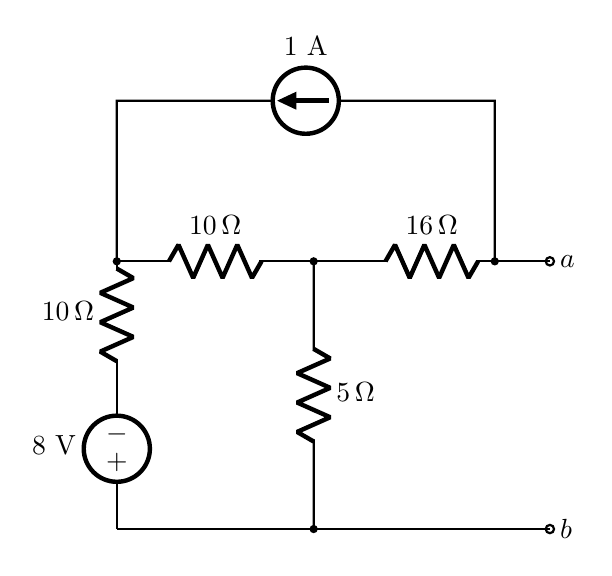
\begin{tikzpicture}[thick, american, y=1.7cm]
    
    % Defining reference terminals 'a' and 'b' on the right side
    \node[right] at (5.5, 2) {$a$};
    \node[right] at (5.5, 0) {$b$};
    
    % Terminals drawing (small open circles)
    \draw (5.5,2) circle (1.5pt);
    \draw (5.5,0) circle (1.5pt);
    
    % Bottom wire from the 5 ohm resistor branch to terminal b
    \draw (0,0) -- (5.5,0);
    
    % Leftmost vertical branch: 8V independent voltage source + 10 ohm resistor
    \draw (0,0) to[V, l=$8\text{ V}$] (0,1.2)
                to[R, l=$10\,\Omega$] (0,2);
                
    % Top central horizontal bridge containing a 10 ohm resistor
    \draw (0,2) to[R, l=$10\,\Omega$] (2.5,2);
    
    % Central vertical branch: 5 ohm resistor down to baseline
    \draw (2.5,2) to[R, l=$5\,\Omega$] (2.5,0);
    
    % Right horizontal resistor branch leading to terminal a
    \draw (2.5,2) to[R, l=$16\,\Omega$] (5.5,2);
    
    % Upper parallel bypass loop containing the 1A independent current source
    % It branches from the top-left node (0,2) up, goes over, and drops right before terminal 'a'
    \draw (0,2) -- (0,3.2)
                to[I, l=$1\text{ A}$, invert] (4.8,3.2)
                -- (4.8,2);

    % Explicit junction connection dots
    \fill (0,2) circle (1.5pt);
    \fill (2.5,2) circle (1.5pt);
    \fill (2.5,0) circle (1.5pt);
    \fill (4.8,2) circle (1.5pt);

\end{tikzpicture}

\end{center}
\mk{10} \yr{EEE 163 | L-1/T-1 | 2020--21}

\item Obtain the Norton equivalent circuit at terminals a--b for the circuit shown below.
\begin{center}
  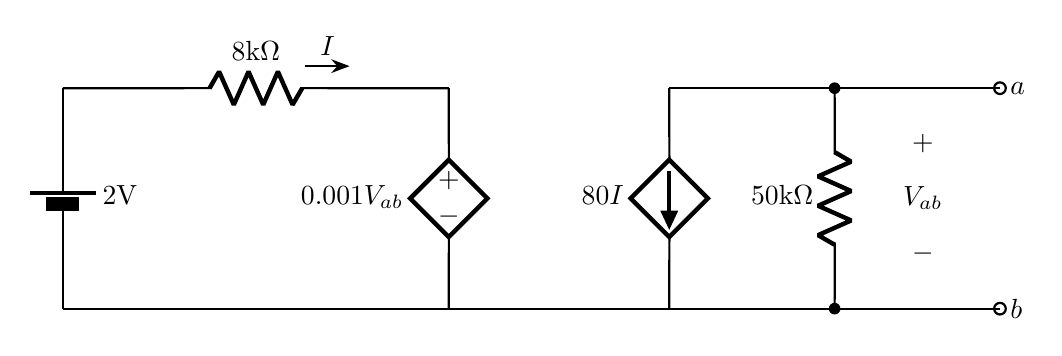
\begin{tikzpicture}[thick, american, scale=1.4]
    
    % Bottom reference rail linking both separate stages
    \draw (0,0) -- (8.5,0);
    
    % --- LEFT STAGE ---
    % 2V DC voltage source (battery style)
    \draw (0,2) to[battery2, l=$2\text{V}$] (0,0);
    
    % 8k ohm horizontal resistor with current indicator I
    \draw (0,2) to[R, l=$8\text{k}\Omega$] (3.5,2);
    \draw[-{Stealth}, thick] (2.2,2.2) -- (2.6,2.2) node[midway, above] {$I$};
    
    % Dependent voltage source controlled by Vab
    \draw (3.5,2) to[cV, l_=$0.001V_{ab}$] (3.5,0);
    
    % --- RIGHT STAGE ---
    % Dependent current source controlled by I
    \draw (5.5,0) to[cI, l=$80I$, invert] (5.5,2);
    
    % Top wire connection for the right side parallel block
    \draw (5.5,2) -- (8.5,2);
    
    % 50k ohm vertical load resistor
    \draw (7,2) to[R, l_=$50\text{k}\Omega$] (7,0);
    
    % --- OUTPUT TERMINALS ---
    \node[right] at (8.5,2) {$a$};
    \node[right] at (8.5,0) {$b$};
    
    \draw (8.5,2) circle (1.5pt);
    \draw (8.5,0) circle (1.5pt);
    
    % Vab open-circuit voltage polarity markings
    \node at (7.8,1.5) {$+$};
    \node at (7.8,1.0) {$V_{ab}$};
    \node at (7.8,0.5) {$-$};

    % Explicit junction connection dots
    \fill (7,2) circle (1.5pt);
    \fill (7,0) circle (1.5pt);

\end{tikzpicture}

\end{center}
\mk{25} \yr{EEE 163 | L-1/T-1 | 2020--21}

\item Find the Norton equivalent circuit across terminal a--b of the circuit below.
\begin{center}
\begin{circuitikz}[scale=1.1, y =1.5cm, thick]
    
    % --- Main Reference Ground Rail ---
    \draw (0,0) to[short] (8,0);
    
    % --- First Branch: 80V Independent DC Voltage Source ---
    \draw (0,0) to[V, invert, l=$80\,\text{V}$] (0,3)
          to[short] (1.5,3);
          
    % --- Second Branch: 30 Ohm Parallel Resistor ---
    \draw (1.5,3) to[R, l=$30\,\Omega$] (1.5,0);
    
    % --- Top Bridge: 40 Ohm Series Resistor ---
    \draw (1.5,3) to[R, l=$40\,\Omega$] (4.5,3);

    % --- Third Branch: 5k Ohm Resistor, 1000V Source, and 6A Current Source ---
    \draw (4.5,3) to[R, l=$5\,\text{k}\Omega$] (4.5,1.8)
          to[V,invert,  l=$1000\,\text{V}$] (4.5,0.9)
          to[I, invert, l=$6\,\text{A}$] (4.5,0);
          
    % Connecting top main rail forward
    \draw (4.5,3) to[short] (6.5,3);

    % --- Fourth Branch: 10 Ohm Parallel Resistor ---
    \draw (6.5,3) to[R, l=$10\,\Omega$] (6.5,0);

    % --- Open Output Terminals (a and b) ---
    \draw (6.5,3) to[short] (8,3)node[ocirc] {} node[right] {$a$};
    \draw (6.5,0) to[short] (8,0) node[ocirc] {} node[right] {$a$};

    % --- Connection Node Dots ---
    \node[circle, fill, inner sep=1.2pt] at (1.5,3) {} ;
    \node[circle, fill, inner sep=1.2pt] at (1.5,0) {};
    \node[circle, fill, inner sep=1.2pt] at (4.5,3) {};
    \node[circle, fill, inner sep=1.2pt] at (4.5,0) {};
    \node[circle, fill, inner sep=1.2pt] at (6.5,3) {};
    \node[circle, fill, inner sep=1.2pt] at (6.5,0) {};

\end{circuitikz}


\end{center}
\mk{20} \yr{EEE 163 | L-1/T-1 | 2018--19}

\item Two networks A and B, composed only of resistors and sources, are connected. Measurements give $V = 1$\,V, $i = 0$\,mA in one connection

\begin{center}
  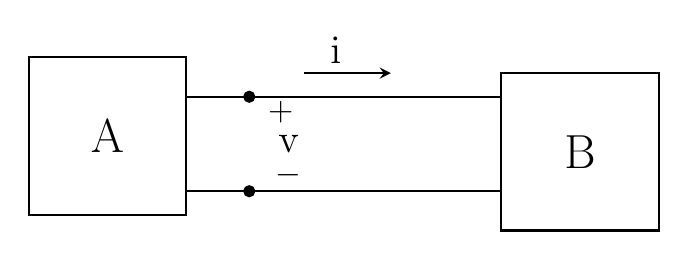
\begin{tikzpicture}[scale=1.0, >=stealth]

    % --- Block A (Left Side) ---
    \draw[thick] (0, 0.5) rectangle (2, 2.5);
    \node[font=\LARGE] at (1, 1.5) {A};

    % --- Block B (Right Side) ---
    \draw[thick] (6, 0.3) rectangle (8, 2.3);
    \node[font=\LARGE] at (7, 1.3) {B};

    % --- Connecting Wires ---
    % Top Wire
    \draw[thick] (2, 2.0) -- (6, 2.0);
    % Bottom Wire
    \draw[thick] (2, 0.8) -- (6, 0.8);

    % --- Terminal Dots ---
    \filldraw (2.8, 2.0) circle (2pt);
    \filldraw (2.8, 0.8) circle (2pt);

    % --- Voltage Label (v) ---
    \node[font=\Large] at (3.3, 1.4) {v};
    \node[font=\large] at (3.2, 1.8) {$+$};
    \node[font=\large] at (3.3, 1.0) {$-$};
    % Curved arrow for voltage orientation


    % --- Current Label (i) with Arrow ---
    % Overhead current tracking line
    \draw[thick] (3.5, 2.3) -- (4.3, 2.3);
    \draw[->, thick] (4.3, 2.3) -- (4.6, 2.3);
    \node[above, font=\Large] at (3.9, 2.3) {i};

\end{tikzpicture}

\end{center}

and $V = 0.5$\,V, $i = 0.5$\,mA in the reversed connection. Determine the Th\'{e}venin equivalent circuits of A and B.
\begin{center}
  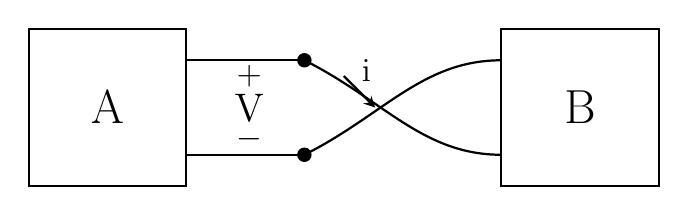
\begin{tikzpicture}[scale=1.0, thick ,>=stealth]

    % --- Block A (Left Side) ---
    \draw[thick] (0, 0.5) rectangle (2, 2.5);
    \node[font=\LARGE] at (1, 1.5) {A};

    % --- Block B (Right Side) ---
    \draw[thick] (6, 0.5) rectangle (8, 2.5);
    \node[font=\LARGE] at (7, 1.5) {B};

    % --- Terminals exiting Block A ---
    \draw[thick] (2, 2.1) -- (3.5, 2.1);
    \draw[thick] (2, 0.9) -- (3.5, 0.9);

    % --- Terminal Connection Dots ---
    \filldraw (3.5, 2.1) circle (2.2pt);
    \filldraw (3.5, 0.9) circle (2.2pt);

    % --- Voltage Label (V) with Polarity ---
    \node[font=\Large] at (2.8, 1.5) {V};
    \node[font=\large] at (2.8, 1.9) {$+$};
    \node[font=\large] at (2.8, 1.1) {$-$};

    % --- Twisted Crossover Wires to Block B ---
    % Top Terminal (3.5, 2.1) connects to Bottom of Block B (6, 0.9)
    \draw[thick] (3.5, 2.1) .. controls (4.5, 1.6) and (5.0, 0.9) .. (6, 0.9);
    
    % Bottom Terminal (3.5, 0.9) connects to Top of Block B (6, 2.1)
    % A small white mask break can be added here if you want an explicit bridge gap,
    % but a clean solid cross matches the hand-drawn style perfectly.
    \draw[thick] (3.5, 0.9) .. controls (4.5, 1.4) and (5.0, 2.1) .. (6, 2.1);

    % --- Current Label (i) with Directional Arrow ---
    % Positioned dynamically along the slope of the upper crossover wire
    \draw[->, thick] (4.0, 1.9) -- (4.4, 1.5);
    \node[above right, font=\large] at (4.1, 1.7) {i};

\end{tikzpicture}

\end{center}

\mk{8} \yr{EEE 163 | L-1/T-1 | 2018--19}

\item Using source transformation, find the value of $V_1$ in the circuit below.
\begin{center}
  \begin{circuitikz}[scale=1.1,thick ]

    % --- Bottom Reference Rail ---
    \draw (0,0) to[short] (10,0);

    % --- Leftmost Branch: 2A Independent Current Source ---
    \draw (0,0) to[I, l=$2\,\text{A}$, v=$V_1$] (0,3)
          to[short] (2,3);

    % --- Second Vertical Branch: 20 Ohm Resistor + 20V Source ---
    \draw (2,3) to[R, l=$20\,\Omega$] (2,1.5)
          to[V, l=$20\,\text{V}$] (2,0);

    % --- Top Main Loop Row: 5 Ohm Resistor & Dependent Voltage Source ---
    \draw (2,3) to[R, l=$5\,\Omega$] (4.5,3)
          to[cV, l=$0.5V_1$] (6,3);

    % --- Third Vertical Branch: 2 Ohm Resistor ---
    \draw (6,3) to[R, l=$2\,\Omega$] (6,0);
    \draw (6,3) to[short] (8,3);

    % --- Fourth Vertical Branch: 10 Ohm Resistor + 10V Source ---
    \draw (8,3) to[R, l=$10\,\Omega$] (8,1.5)
          to[V, l=$10\,\text{V}$] (8,0);
    \draw (8,3) to[short] (10,3);

    % --- Rightmost Branch: 4A Independent Current Source ---
    \draw (10,0) to[I, l=$4\,\text{A}$] (10,3);

    % --- Connection Node Dots ---
    \node[circle, fill, inner sep=1.2pt] at (2,3) {};
    \node[circle, fill, inner sep=1.2pt] at (2,0) {};
    \node[circle, fill, inner sep=1.2pt] at (6,3) {};
    \node[circle, fill, inner sep=1.2pt] at (6,0) {};
    \node[circle, fill, inner sep=1.2pt] at (8,3) {};
    \node[circle, fill, inner sep=1.2pt] at (8,0) {};

\end{circuitikz}

\end{center}
\mk{20} \yr{EEE 163 | L-1/T-1 | 2018--19}

\item For the circuit shown below, find $R_1$ so that maximum power will be transferred from the left of section a--b to the right of section a--b. What is that power?
\begin{center}
  \begin{circuitikz}[scale=1.1, thick]

    % --- Lower Reference Rail & Control Current ia ---
    \draw (0,0) to[short, i_=$i_a$, -*] (3,0) coordinate (BottomLeftJunc)
          to[short, -o] (4.5,0) node[below=2pt] {$b$};
          
    \draw (4.5,0) to[short, o-*] (7,0) coordinate (BottomMidJunc)
                  to[short] (8.5,0);

    % --- Leftmost Section: 12V Battery & Series 6 Ohm Resistor ---
    \draw (0,0) to[battery2,invert,  l=$12\,\text{V}$] (0,2.5)
          to[R, l=$6\,\Omega$, -*] (3,2.5) coordinate (TopLeftJunc);

    % --- Central Left Branch: Dependent Voltage Source (5ia) ---
    \draw (TopLeftJunc) to[cV, l_=$5i_a$] (BottomLeftJunc);

    % --- Central Open Interface Section ---
    % Branch leading to open terminal 'a'
    \draw (TopLeftJunc) to[R, l=$3\,\Omega$, -o] (4.5,2.5) node[above=2pt] {$a$};
    
    % Branch continuing from terminal 'a' through R1
    \draw (4.5,2.5) to[short, o-] (4.5,2.5) 
                    to[R, l=$R_1$, -*] (7,2.5) coordinate (TopMidJunc);

    % --- Right Network Ladder Stage ---
    % Shunt 1 Ohm Resistor
    \draw (TopMidJunc) to[R, l=$1\,\Omega$] (BottomMidJunc);

    % Rightmost Series 0.5 Ohm and Shunt 2 Ohm Loop
    \draw (TopMidJunc) to[R, l=$0.5\,\Omega$] (8.5,2.5)
                       to[R, l=$2\,\Omega$] (8.5,0)
                       to[short] (BottomMidJunc);

\end{circuitikz}

\end{center}
\mk{15} \yr{EEE 163 | L-1/T-1 | 2018--19}

\item Find $V_x$ by applying series of source transformations for the circuit below.
\begin{center}
  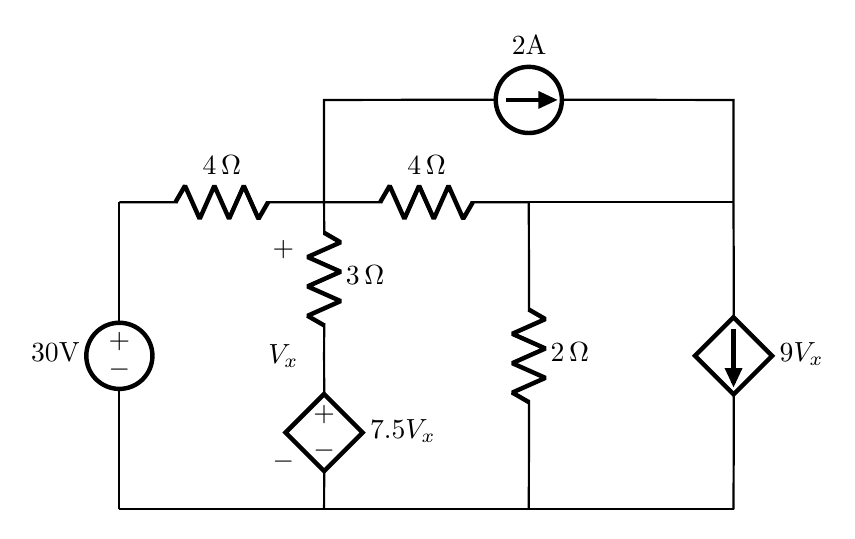
\begin{tikzpicture}[american, thick, scale=1.3]
    % Ground/Reference Node line at the bottom
    \draw (0,0) -- (6,0);
    
    % Leftmost branch with 30V independent voltage source
    \draw (0,0) to[V, l=30V, invert] (0,3);
    
    % Top-left 4 ohm resistor
    \draw (0,3) to[R, l=4\ enclosures=none, l=$4\,\Omega$] (2,3);
    
    % Node definitions for clarity
    % Node 1 is at (2,3), Node 2 is at (4,3), Node 3 is at (6,3)
    
    % Middle branch with 3 ohm resistor and 7.5Vx dependent voltage source
    % Also marking the Vx polarity across this entire branch
    \draw (2,3) to[R, l=$3\,\Omega$] (2,1.5)
                to[cV, l=$7.5V_x$] (2,0);
                
    % Top middle 4 ohm resistor
    \draw (2,3) to[R, l=$4\,\Omega$] (4,3);
    % 2A independent current source bridging from Node 1 to Node 3
    \draw (2,3) -- (2,4)
                to[I, l=2A] (6,4)
                -- (6,3);
     \draw (1.6,3) to[open ,v=$V_x$] (1.6,0);           
    % 2 ohm resistor branch
    \draw (4,3) to[R, l=$2\,\Omega$] (4,0);
    
    % Connection between Node 2 and Node 3
    \draw (4,3) -- (6,3);
    
    % Rightmost branch with 9Vx dependent current source
    \draw (6,3) to[cI, l=$9V_x$] (6,0);

\end{tikzpicture}


\end{center}
\mk{15} \yr{EEE 163 | L-1/T-1 | 2018--19}

\item Using superposition theorem, find the Th\'{e}venin equivalent between terminals a--b of the circuit shown below.
\begin{center}
  \begin{circuitikz}[thick ,scale=1.2]
    % --- Main Ground / Bottom Rail ---
    \draw (0,0) to[short, -*] (3,0) 
                to[short, -*] (4.5,0) 
                to[short, -*] (6,0);
        
    % --- Left-most Branch ---
    % 10V Voltage Source
    \draw (0,0) to[V,invert,  l=$10\text{ V}$] (0,6)
          to[R, l=$10\,\Omega$] (6,6);
        
    % --- Right Vertical Resistor Spine ---
    \draw (6,6) to[R, l=$20\,\Omega$] (6,5) node[circle, fill, inner sep=1.5pt] (nodeA) {};
    \draw (6,5) to[R, l=$30\,\Omega$] (6,3.5) node[circle, fill, inner sep=1.5pt] (nodeB) {};
    \draw (6,3.5) to[R, l=$40\,\Omega$] (6,1.5) node[circle, fill, inner sep=1.5pt] (nodeC) {};
    \draw (6,1.5) to[R, l=$50\,\Omega$] (6,0);
        
    % --- Output Terminals a and b ---
    \draw (6,5) to[short, -o] (7.5,5) node[right] {$a$};
    \draw (6,3.5) to[short, -o] (7.5,3.5) node[right] {$b$};
        
    % --- Internal Parallel Sources ---
    % 5A Current Source (pointing up)
    \draw (3,0) to[I, l=$5\text{ A}$] (3,3.5) -- (6,3.5);
    
    % 7A Current Source (pointing down)
    \draw (6,5) -- (4.5,5) to[I, l=$7\text{ A}$] (4.5,3.5);
        
    % 5V Voltage Source (+ on top)
    \draw (4.5,0) to[V,invert,  l=$5\text{ V}$] (4.5,1.5) -- (6,1.5);
        
\end{circuitikz}

\end{center}
\mk{18} \yr{EEE 163 | L-1/T-1 | 2017--18}

\item Determine the maximum power available from the black box.
\begin{center}
  \begin{circuitikz}[thick, scale=1.2]
    
    % --- Black Box ---
    \draw[thick] (0, 0) rectangle (2.5, 4) node[midway, align=center] {Black \\ box};
    
    % --- Top and Bottom Rails (Left to Voltmeter) ---
    \draw (2.5, 3.2) -- (4.5, 3.2);
    \draw (2.5, 0.8) -- (4.5, 0.8);
    
    % --- Voltmeter (Parallel) ---
    \draw (4.5, 3.2) to[rmeter, t=V] (4.5, 0.8);
    
    % --- Ammeter (Series) & Top Wire ---
    \draw (4.5, 3.2) to[rmeter, t=A] (7.5, 3.2) -- (8.5, 3.2);
    
    % --- Current Indicator Arrow ---
    % Drawn slightly above the top wire to match the diagram
    \draw[-latex, thick] (7.2, 3.6) -- (8.2, 3.6) node[midway, above] {$I$};
    
    % --- Bottom Return Wire ---
    \draw (4.5, 0.8) -- (8.5, 0.8);
    
    % --- Variable Resistor ---
    \draw (8.5, 3.2) to[vR, l=$R$] (8.5, 0.8);
   
\end{circuitikz}
\vspace{0.5cm}
    \begin{tabular}{ccc}
        \toprule
        $\mathbf{R(\Omega)}$ & $\mathbf{V(V)}$ & $\mathbf{i(A)}$ \\ 
        \midrule
        2  & 3    & 1.5  \\
        8  & 8    & 1.0  \\
        14 & 10.5 & 0.75 \\ 
        \bottomrule
    \end{tabular} 
\end{center}
\mk{10} \yr{EEE 163 | L-1/T-1 | 2017--18}

\item Consider the following $n$-bit R-2R Ladder DAC circuit below. Suppose only switch SW$_n$ is connected to $V_r$ volts and all other switches are connected to GND. (i)~Find the Th\'{e}venin equivalent of the dashed box at node $a_n$. (ii)~Extend the box to include node $a_{n-1}$ and find the new Th\'{e}venin equivalent. (iii)~Deduce the voltage at node $a_1$ and hence find the output of the Op-Amp, $V_o$.
\begin{center}
  \begin{circuitikz}[thick, scale=0.8, transform shape]

    % --- Voltage Rails ---
    % VR Rail (Top)
    \draw (-1.5, 5) node[left]{$V_R+$} -- (10.5, 5);
    
    % GND Rail (Middle)
    \draw (-1.5, 4) node[left]{GND} node[ground]{} -- (10.5, 4);

    % --- Dashed Box (n-th stage) ---
    \draw[dashed, thick] (-0.5, -1) rectangle (3.2, 3.5);

    % --- Main Ground & Initial Resistor ---
    \draw (0,-0.5) node[ground]{} -- (0,0);
    \draw (0,0) to[R, l=$2R$] (2,0) node[circle, fill, inner sep=1.2pt]{} node[below=3pt]{$a_n$};

    % --- Stage n ---
    % Vertical branch
    \draw (2,0) to[R, l=$2R$] (2,2) node[circle, fill, inner sep=1.2pt](pn){};
    \node[right] at (2, 2.5) {$SW_n$};
    
    % Switch connections to VR (left) and GND (right)
    \draw (1.6, 3) node[circle, draw, inner sep=1.2pt, fill=white]{} -- (1.6, 3.8);
    \draw[white, line width=3.5pt] (1.6, 3.8) -- (1.6, 4.2); % Erase behind jump
    \draw (1.6, 3.8) arc(-90:90:0.2); % Jump over GND rail
    \draw (1.6, 4.2) -- (1.6, 5) node[circle, fill, inner sep=1.2pt]{};
    
    \draw (2.4, 3) node[circle, draw, inner sep=1.2pt, fill=white]{} -- (2.4, 4) node[circle, fill, inner sep=1.2pt]{};
    \draw[thick, -latex] (pn) -- (1.65, 2.85); % Arrow pointing to VR connection

    % --- Between n and n-1 ---
    \draw (2,0) to[R, l=$R$] (4,0) node[circle, fill, inner sep=1.2pt]{} node[below=3pt]{$a_{n-1}$};

    % --- Stage n-1 ---
    \draw (4,0) to[R, l=$2R$] (4,2) node[circle, fill, inner sep=1.2pt](pn1){};
    \node[right] at (4, 2.5) {$SW_{n-1}$};
    
    \draw (3.6, 3) node[circle, draw, inner sep=1.2pt, fill=white]{} -- (3.6, 3.8);
    \draw[white, line width=3.5pt] (3.6, 3.8) -- (3.6, 4.2);
    \draw (3.6, 3.8) arc(-90:90:0.2);
    \draw (3.6, 4.2) -- (3.6, 5) node[circle, fill, inner sep=1.2pt]{};
    
    \draw (4.4, 3) node[circle, draw, inner sep=1.2pt, fill=white]{} -- (4.4, 4) node[circle, fill, inner sep=1.2pt]{};
    \draw[thick, -latex] (pn1) -- (3.65, 2.85);

    % --- Gap with Dots ---
    \draw (4,0) to[R, l=$R$] (5.5,0);
    \draw[loosely dotted, thick] (5.5,0) -- (6.5,0);
    \draw (6.5,0) -- (7,0) node[circle, fill, inner sep=1.2pt]{} node[below=3pt]{$a_2$};

    % --- Stage 2 ---
    \draw (7,0) to[R, l=$2R$] (7,2) node[circle, fill, inner sep=1.2pt](p2){};
    \node[right] at (7, 2.5) {$SW_2$};
    
    \draw (6.6, 3) node[circle, draw, inner sep=1.2pt, fill=white]{} -- (6.6, 3.8);
    \draw[white, line width=3.5pt] (6.6, 3.8) -- (6.6, 4.2);
    \draw (6.6, 3.8) arc(-90:90:0.2);
    \draw (6.6, 4.2) -- (6.6, 5) node[circle, fill, inner sep=1.2pt]{};
    
    \draw (7.4, 3) node[circle, draw, inner sep=1.2pt, fill=white]{} -- (7.4, 4) node[circle, fill, inner sep=1.2pt]{};
    \draw[thick, -latex] (p2) -- (6.65, 2.85);

    % --- Between 2 and 1 ---
    \draw (7,0) to[R, l=$R$] (9,0) node[circle, fill, inner sep=1.2pt]{} node[below=3pt]{$a_1$};

    % --- Stage 1 ---
    \draw (9,0) to[R, l=$2R$] (9,2) node[circle, fill, inner sep=1.2pt](p1){};
    \node[right] at (9, 2.5) {$SW_1$};
    
    \draw (8.6, 3) node[circle, draw, inner sep=1.2pt, fill=white]{} -- (8.6, 3.8);
    \draw[white, line width=3.5pt] (8.6, 3.8) -- (8.6, 4.2);
    \draw (8.6, 3.8) arc(-90:90:0.2);
    \draw (8.6, 4.2) -- (8.6, 5) node[circle, fill, inner sep=1.2pt]{};
    
    \draw (9.4, 3) node[circle, draw, inner sep=1.2pt, fill=white]{} -- (9.4, 4) node[circle, fill, inner sep=1.2pt]{};
    \draw[thick, -latex] (p1) -- (8.65, 2.85);

    % --- Op-Amp & Output Stage ---
    % Op-amp placement (inverting input aligned to y=0)
    \node[op amp] (OA) at (11.5, -0.5) {};
    
    % Connect a1 to inverting (-) input
    \draw (9,0) -- (OA.-) node[circle, fill, inner sep=1.2pt, pos=0.85](fb_dot){};
    
    % Connect non-inverting (+) input to ground
    \draw (OA.+) -- ++(0,-0.5) node[ground]{};

    % Feedback Resistor (Rf)
    \draw (fb_dot) -- ++(0, 1.8) to[R, l=$R_f$] ++(2.8,0) -| (OA.out) node[circle, fill, inner sep=1.2pt]{};

    % Output terminals (vo)
    \draw (OA.out) to[short, -o] ++(1,0) node[above left]{$+$} node[right]{$v_o$};
    \draw (OA.out) ++(1,-1.5) node[ground]{} -- ++(0,0.5) node[circle, draw=none, inner sep=0pt](gnd_term){} to[short, -o] ++(0,1) node[below left]{$-$};

\end{circuitikz}

\end{center}
\vspace{0.5cm}
\begin{center}
  \begin{circuitikz}[thick, scale=1.2, transform shape]
    
    % --- Dashed Bounding Box ---
    \draw[dashed, thick] (-0.5, -1.2) rectangle (7.5, 4.5);
    
    % --- Thevenin Equivalent Block ---
    \draw[thick] (0, 0) rectangle (2.5, 2) node[midway, align=center] {Thevenin \\ Equivalent \\ input (i)};
    
    % --- Box Ground Connection ---
    \draw (1.25, 0) -- (1.25, -0.6) node[ground]{};
    
    % --- Node a_n ---
    \draw (2.5, 1) -- (3.5, 1) node[circle, fill, inner sep=1.2pt]{} node[above left]{$a_n$};
    
    % --- Series Resistor R ---
    \draw (3.5, 1) to[R, l=$R$] (6, 1) node[circle, fill, inner sep=1.2pt]{} node[below=3pt]{$a_{n-1}$};
    
    % --- Rightward Continuation Wire ---
    \draw (6, 1) -- (7, 1);
    
    % --- Vertical Resistor 2R ---
    \draw (6, 1) -- (6, 1.8) to[R, l_=$2R$] (6, 3.1) node[circle, fill, inner sep=1.2pt](switch_pivot){} ;
    
    % --- Switch Terminals (Gnd and +VR) ---
    % Left Terminal (Gnd)
    \draw (5.4, 3.8) node[circle, draw, inner sep=1.2pt, fill=white]{} -- (5.4, 4.2) node[above]{Gnd};
    
    % Right Terminal (+VR)
    \draw (6.6, 3.8) node[circle, draw, inner sep=1.2pt, fill=white]{} -- (6.6, 4.2) node[above]{$+V_R$};
    
    % --- Switch Lever Arrow ---
    \draw[thick, -latex] (switch_pivot) -- (5.5, 3.7);
    
\end{circuitikz}

\end{center}
\mk{18} \yr{EEE 163 | L-1/T-1 | 2017--18}

\item Use superposition principle to find the voltage $V_{ab}$. Then, find the Th\'{e}venin and Norton equivalent of the circuit between terminals a and b below.
\begin{center}
  \begin{circuitikz}[thick, scale=1.2]
    % --- Terminals a and b ---
    \draw (0,2) node[left, font=\bfseries] {a} to[short, o-] (2,2);
    \draw (8,2) to[short, -o] (10,2) node[right, font=\bfseries] {b};

    % --- Central Horizontal Path ---
    % 18V Voltage source
    \draw (2,2) to[V, l=$18\text{V}$] (4,2);
    
    % 4 Ohm resistor
    \draw (4,2) to[R, l=$4\,\Omega$] (6,2);
    
    % 6 Ohm resistor
    \draw (6,2) to[R, l=$6\,\Omega$] (8,2);

    % --- Parallel 3A Current Source (Below the 4 Ohm resistor) ---
    % Drawn from right to left (6 to 4) so the arrow points left
    \draw (4,2) -- (4,1)
          (6,2) -- (6,1) to[I, l=$3\text{A}$] (4,1);

    % --- Top Outer Loop ---
    % 2A Current source pointing right
    \draw (2,2) -- (2,3.5)
          to[I, l=$2\text{A}$] (8,3.5)
          -- (8,2);

    % --- Bottom Outer Loop ---
    % 10V Voltage source and 5 Ohm resistor in series
    \draw (2,2) -- (2,0)
          to[V, l=$10\text{V}$] (5,0)
          to[R, l=$5\,\Omega$] (8,0)
          -- (8,2);

\end{circuitikz}

\end{center}
\mk{20} \yr{EEE 163 | L-1/T-1 | 2015--16}

\item Find the value of resistance $R$ so that maximum power is transferred to the 3\,k$\Omega$ resistance. Find the value of that maximum power.
\begin{center}
  \begin{circuitikz}[scale=1.2, thick]
    % --- Left Loop ---
    % 16V independent voltage source
    \draw (0,2.5) to[V, l=$16\text{V}$] (0,0);
    
    % Top wire carrying current I_x
    \draw (0,2.5) to[short, i^=$I_x$] (2.5,2.5);
    
    % Bottom wire containing the 2k Ohm resistor
    \draw (0,0) to[R, l_=$2\text{k}\Omega$] (2.5,0);
    
    % 9mA independent current source pointing upwards
    \draw (2.5,0) to[I, l_=$9\text{mA}$] (2.5,2.5);
    
    % --- Middle to Right Section ---
    % Dependent current source 10I_x pointing right
    \draw (2.5,2.5) to[cI, l=$10I_x$] (5.5,2.5);
    
    % Bottom connecting wire
    \draw (2.5,0) -- (5.5,0);
    
    % Vertical resistor R
    \draw (5.5,2.5) to[R, l_=$R$] (5.5,0);
    
    % --- Rightmost Loop ---
    % 3k Ohm parallel resistor loop completion
    \draw (5.5,2.5) -- (7.5,2.5)
          to[R, l_=$3\text{k}\Omega$] (7.5,0)
          -- (5.5,0);

\end{circuitikz}

\end{center}
\mk{13} \yr{EEE 163 | L-1/T-1 | 2015--16}

\item Find $V_x$ by applying a series of source transformations for the circuit below.
\begin{center}
  \begin{circuitikz}[thick, y=1.6cm, x=1.4cm]
    % --- Ground / Bottom Reference Line ---
    \draw (0,0) -- (7,0);

    % --- Left Side ---
    % 30V independent voltage source
    \draw (0,2) to[V, l=$30\text{V}$] (0,0);

    % First horizontal 4 Ohm resistor
    \draw (0,2) to[R, l=$4\,\Omega$] (2,2);

    % --- Central Branch ---
    % 3 Ohm resistor in series with 7.5Vx dependent voltage source
    \draw (2,2) to[R, l=$3\,\Omega$] (2,1)
          to[cV, l=$7.5V_x$] (2,0);

    % Manual placement of Vx polarity markings across the whole central branch
    \node[below left=2pt] at (2,2) {$+$};
    \node[above left=2pt] at (2,0) {$-$};
    \node[left=6pt] at (2,0.8) {$V_x$};

    % --- Right Side ---
    % Second horizontal 4 Ohm resistor
    \draw (2,2) to[R, l=$4\,\Omega$] (5,2);

    % Vertical 2 Ohm resistor
    \draw (5,2) to[R, l=$2\,\Omega$] (5,0);

    % Connection to the final branch
    \draw (5,2) -- (7,2);

    % Rightmost vertical dependent current source 9Vx
    \draw (7,2) to[cI, l=$9V_x$] (7,0);

    % --- Overhead Bridge ---
    % 2A independent current source bypassing the middle section
    \draw (2,2) -- (2,3.3)
          to[I, l=$2\text{A}$] (7,3.3)
          -- (7,2);

\end{circuitikz}

\end{center}
\mk{12} \yr{EEE 163 | L-1/T-1 | 2015--16}

\item The device shown below is represented by a Norton equivalent circuit. When a resistor of 5\,k$\Omega$ is connected across the device, $V_o = 5 - j15$\,V. When a capacitor of $-j3\,\Omega$ is connected across the device, $I_o = 4.5 - j6$\,mA. Find the Norton current $I_N$ and the Norton impedance $Z_N$.
\begin{center}
  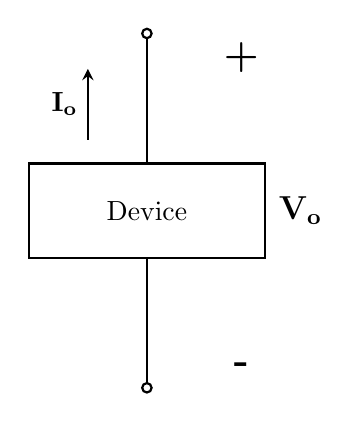
\begin{tikzpicture}[thick, scale=1.5, >=stealth]
    % --- Device Box ---
    \draw[thick] (-1, 0.5) rectangle (1, 1.3);
    \node[font=\rmfamily] at (0, 0.9) {Device};

    % --- Terminals and Connecting Wires ---
    % Top wire and open circle terminal
    \draw[thick] (0, 1.3) -- (0, 2.4) node[circle, draw, inner sep=1.2pt, fill=white] {};
    % Bottom wire and open circle terminal
    \draw[thick] (0, 0.5) -- (0, -0.6) node[circle, draw, inner sep=1.2pt, fill=white] {};

    % --- Current Arrow (Io) ---
    \draw[->, thick] (-0.5, 1.5) -- (-0.5, 2.1);
    \node[left, font=\bfseries\rmfamily] at (-0.5, 1.8) {I\textsubscript{o}};

    % --- Voltage Signs and Label (Vo) ---
    \node[font=\bfseries\Large] at (0.8, 2.2) {+};
    \node[font=\bfseries\Large] at (0.8, -0.4) {-};
    \node[font=\bfseries\rmfamily\large] at (1.3, 0.9) {V\textsubscript{o}};

\end{tikzpicture}

\end{center}
\mk{20} \yr{EEE 163 | L-1/T-1 | 2015--16}

\item Find the Th\'{e}venin equivalent of the circuit shown below at terminal `ab'.
\begin{center}
  \begin{circuitikz}[scale=1.2, transform shape, thick]

    % Far left branch: 4V independent voltage source (+ on top)
    \draw (0,3) to[V, l=$4\mathrm{V}$] (0,0);

    % Top left horizontal branch: 5 Ohm resistor
    \draw (0,3) to[R, l=$5\,\Omega$] (3,3);

    % Bottom left horizontal return wire
    \draw (0,0) -- (3,0);

    % Central vertical branch: 10 Ohm resistor
    \draw (3,3) to[R, l=$10\,\Omega$] (3,0);

    % Ground connection at the central bottom junction
    \draw (3,0) node[ground]{};

    % Top middle parallel section
    % Bottom path of parallel section: 5 Ohm resistor
    \draw (3,3) to[R, l=$5\,\Omega$] (6,3);
    
    % Top path of parallel section: Dependent current source (5Vx) pointing right
    \draw (3,3) -- (3,4.5) to[cI, l=$5V_x$] (6,4.5) -- (6,3);

    % Top right horizontal branch: 2V independent voltage source (+ on left)
    \draw (6,3) to[V, l=$2\mathrm{V}$] (8,3);

    % Terminals 'a' and 'b' extending to the right
    \draw (8,3) to[short, -o] (9,3) node[above]{a};
    \draw (8,0) to[short, -o] (9,0) node[below]{b};

    % Variable load resistor R_L connected between terminals a and b
    \draw (9,3) to[vR, l=$R_L$] (9,0);

    % Bottom right horizontal branch: 10 Ohm resistor with voltage Vx (+ on left)
    \draw (3,0) to[R, l=$10\,\Omega$, v_=$V_x$] (8,0);

\end{circuitikz}

\end{center}
\mk{17} \yr{EEE 163 | L-1/T-1 | 2014--15}

\item In an experiment, the circuit shown below was used to find the value of unknown resistance $R$. The load resistance $R_L$ was varied and the corresponding power dissipation in that resistor was measured. At $R_L = 25\,\Omega$, a maximum power dissipation of 16\,W was found in that resistor. What was the value of $R$?
\begin{center}
  \begin{circuitikz}[scale=1.2, transform shape, thick]

    % Far left branch: 90V independent voltage source (+ on top)
    \draw (0,0) to[V,invert, l=$90\mathrm{V}$] (0,3);

    % Top horizontal wire (left): Resistor R
    \draw (0,3) to[R, l=$R$] (3,3);

    % Bottom wire (left)
    \draw (0,0) -- (3,0);

    % Middle vertical branch 1: 120 Ohm resistor
    \draw (3,3) to[R, l=$120\,\Omega$] (3,0);
    
    % Ground connection
    \draw (3,0) node[ground]{};

    % Top horizontal wire (middle): 20 Ohm resistor with current Ix
    \draw (3,3) to[R, l=$20\,\Omega$, i_=$I_x$] (6,3);

    % Middle vertical branch 2: 20 Ohm resistor and dependent voltage source (20Ix)
    \draw (6,3) to[R, l=$20\,\Omega$] (6,1.5);
    \draw (6,1.5) to[cV, l=$20I_x$] (6,0);

    % Bottom wire (right)
    \draw (3,0) -- (6,0);

    % Terminals leading to the load
    \draw (6,3) to[short, -o] (8,3);
    \draw (6,0) to[short, -o] (8,0);

    % Far right load branch: Variable resistor R_L
    \draw (8,3) to[vR, l=$R_L$] (8,0);


\end{circuitikz}

\end{center}
\mk{18} \yr{EEE 163 | L-1/T-1 | 2014--15}

\item Find $v_0$ using superposition theorem for the circuit shown below.
\begin{center}
  \begin{circuitikz}[scale=1.2, transform shape, thick]

    % Far left branch: 100V independent voltage source (+ on top)
    \draw (0,4) to[V, l=$100\mathrm{V}$] (0,0);

    % Top wire for the left section
    \draw (0,4) -- (5.5,4);

    % First middle vertical branch (120 Ohm and 60 Ohm resistors)
    \draw (2.5,4) to[R, l_=$120\,\Omega$] (2.5,2);
    \draw (2.5,2) to[R, l_=$60\,\Omega$] (2.5,0);

    % Horizontal cross branch with 2A independent current source
    \draw (2.5,2) to[I, l=$2\mathrm{A}$] (5.5,2);

    % Second middle vertical branch (30 Ohm and 30 Ohm resistors)
    \draw (5.5,4) to[R, l=$30\,\Omega$] (5.5,2);
    \draw (5.5,2) to[R, l=$30\,\Omega$, v_=$V_x$] (5.5,0);

    % Ground connection on the common bottom wire
    \draw (6.75,0) node[ground]{};

    % Right isolated section (Dependent voltage source loop)
    % 2Vx Dependent Voltage Source (drawing from bottom to top, + on top)
    \draw (8,3) to[cV, l_=$2V_x$] (8,0);
    
    % Top horizontal 20 Ohm resistor
    \draw (8,3) to[R, l=$20\,\Omega$] (11,3);

    % Far right vertical 80 Ohm resistor with voltage Vo (+ on top)
    \draw (11,3) to[R, l=$80\,\Omega$, v=$V_o$] (11,0);

    % Continuous bottom return wire connecting all bottom nodes
    \draw (0,0) -- (11,0);

\end{circuitikz}

\end{center}
\mk{15} \yr{EEE 163 | L-1/T-1 | 2014--15}

\item In an AC circuit, show that the maximum average power is transferred to the load when the load impedance $Z_L$ equals the complex conjugate of the Th\'{e}venin impedance $Z_{Th}$. Also find the maximum average power $P_{max}$ at this condition.
\mk{15} \yr{EEE 163 | L-1/T-1 | 2014--15}

\item Find the Norton equivalent circuit with respect to the terminals a, b for the circuit shown below. For maximum average power transfer if a purely resistive load is connected across terminals a and b, what will be its value?
\begin{center}
  \begin{circuitikz}[scale=1.2, transform shape, thick]

    % Left-most branch: AC Voltage Source Vs = 25 \angle 0° V
    \draw (0,0) to[vsourcesin, l=$V_s {=} 25\angle 0^\circ\mathrm{V}$] (0,3);

    % Top left horizontal path: 1 kOhm resistor carrying current I_phi
    \draw (0,3) to[R, l=$1\,\mathrm{k}\Omega$, i=$I_\phi$] (3,3);

    % First vertical dependent branch: Dependent Voltage Source 4V_2 (+ on top)
    \draw (3,3) to[cV, l=$4V_2$, n=vsnode] (3,0);

    % Top middle horizontal path: Capacitor -j250 Ohm
    \draw (3,3) to[C, l=$-j250\,\Omega$] (6,3);

    % Second vertical dependent branch: Dependent Current Source I_phi (pointing down)
    \draw (6,3) to[cI, l=$I_\phi$] (6,0);

    % Far right vertical branch: 50 Ohm resistor with voltage V_2 (+ on top)
    \draw (8,3) to[R, l=$50\,\Omega$, v=$V_2$] (8,0);

    % Upper horizontal extension to terminal 'a'
    \draw (6,3) -- (8,3) to[short, -o] (9,3) node[right]{a};

    % Lower continuous return wire and extension to terminal 'b'
    \draw (0,0) -- (8,0) to[short, -o] (9,0) node[right]{b};


\end{circuitikz}

\end{center}
\mk{20} \yr{EEE 163 | L-1/T-1 | 2014--15}

\item Apply superposition theorem to determine the Th\'{e}venin voltage between nodes a and b in the circuit below. Then calculate the Th\'{e}venin equivalent resistance and draw the Norton's equivalent circuit.
\begin{center}
  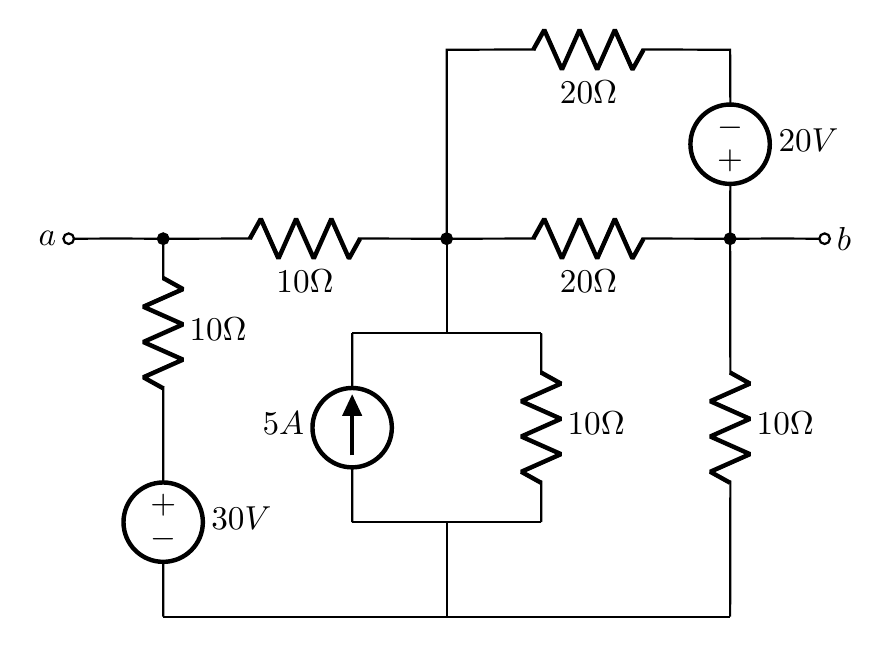
\begin{tikzpicture}[thick,american, scale=1.2, transform shape]

    % Terminals 'a' and 'b'
    \draw (0.5,4) node[left] {$a$} to[short, o-] (1.5,4);
    \draw (7.5,4) to[short, -o] (8.5,4) node[right] {$b$};

    % Main upper nodes
    \node[circ] at (1.5,4) {};
    \node[circ] at (4.5,4) {};
    \node[circ] at (7.5,4) {};

    % Top horizontal branches
    \draw (1.5,4) to[R, l_=$10\Omega$] (4.5,4);
    \draw (4.5,4) to[R, l_=$20\Omega$] (7.5,4);

    % Topmost loop
    \draw (4.5,4) -- (4.5,6) 
          to[R, l_=$20\Omega$] (7.5,6) 
          to[V,invert, l=$20V$] (7.5,4);

    % Leftmost vertical branch
    % Drawn top-to-bottom so the voltage source '+' is at the top
    \draw (1.5,4) to[R, l=$10\Omega$] (1.5,2)
          to[V, l=$30V$] (1.5,0);

    % Rightmost vertical branch
    \draw (7.5,4) to[R, l=$10\Omega$] (7.5,0);

    % Middle vertical section with parallel sub-branches
    \draw (4.5,4) -- (4.5,3);
    \draw (3.5,3) -- (5.5,3);
    
    % Left sub-branch: 5A Current Source (drawn bottom-up for upward arrow)
    \draw (3.5,1) to[I, l=$5A$] (3.5,3);
    
    % Right sub-branch: 10 ohm Resistor (drawn top-down)
    \draw (5.5,3) to[R, l=$10\Omega$] (5.5,1);
    
    \draw (3.5,1) -- (5.5,1);
    \draw (4.5,1) -- (4.5,0);

    % Bottom horizontal connecting wire
    \draw (1.5,0) -- (7.5,0);

\end{tikzpicture}
\end{center}
\mk{20} \yr{EEE 163 | L-1/T-1 | 2013--14}

\item Calculate $v_1$ in the circuit below using source transformation.
\begin{center}
  \begin{circuitikz}[scale=1.2, transform shape, thick]

    % Bottom ground wire
    \draw (0,0) -- (11,0);

    % Branch 1 (Leftmost): 10V independent voltage source and 5 Ohm resistor
    \draw (0,0) to[R, l=$5\,\Omega$] (0,2)
          to[V, l=$10\mathrm{V}$, invert] (0,4);

    % Branch 2: 5 Ohm parallel resistor
    \draw (2,0) to[R, l=$5\,\Omega$, *-*] (2,4);

    % Top wire (left section)
    \draw (0,4) -- (4,4);

    % Branch 3: Dependent voltage source and 2 Ohm resistor
    \draw (4,0) to[R, a=$2\,\Omega$, *-] (4,2)
          to[cV, a=$2v_1$, invert, -*] (4,4);

    % Series resistor between the two sections
    \draw (4,4) to[R, v=$v_1$] (7,4);

    % Branch 4: 5A independent current source
    \draw (7,0) to[I, l=$5\mathrm{A}$, *-*] (7,4);

    % Branch 5: 5 Ohm parallel resistor
    \draw (9,0) to[R, l=$5\,\Omega$, *-*] (9,4);

    % Branch 6 (Rightmost): Dependent current source
    \draw (11,0) to[cI, l=$2v_1$] (11,4);

    % Top wire (right section)
    \draw (7,4) -- (11,4);


\end{circuitikz}

\end{center}
\mk{15} \yr{EEE 163 | L-1/T-1 | 2013--14}

\item State and prove the maximum power transfer theorem.
\mk{10} \yr{EEE 163 | L-1/T-1 | 2013--14}

\item Use a wye-delta transformation to find the branch currents $i_1$, $i_2$ and the power delivered by the current source in the circuit shown below.
\begin{center}
  \begin{circuitikz}[scale=1.2, transform shape, thick]
    % Ground / Bottom reference wire
    \draw (0,0) -- (11,0);
    
    % Leftmost branch: 13A current source pointing upwards
    \draw (0,0) to[I, l=13~A] (0,3) -- (2,3);
    
    % Node 1 vertical branch: 40 ohm resistor with downward current i1
    \draw (2,3) to[R, l=40~$\Omega$, i=$i_1$] (2,0);
    
    % Top wire loop: 25 ohm resistor
    \draw (2,3) -- (2,5.5) to[R, l=25~$\Omega$] (8,5.5);
    
    % Node 1 to Node 2: 100 ohm resistor
    \draw (2,3) to[R, l=100~$\Omega$] (5,3);
    
    % Node 2 vertical branch: 10 ohm resistor with downward current i2
    \draw (5,3) to[R, l=10~$\Omega$, i=$i_2$] (5,0);
    
    % Node 2 to Node 3: 125 ohm resistor
    \draw (5,3) to[R, l=125~$\Omega$] (8,3);
    
    % Node 3 central vertical branch: 20 ohm resistor and vertical connection
    \draw (8,5.5) -- (8,3) to[R, l=20~$\Omega$] (8,0);
    
    % Top-right branch: 50 ohm resistor
    \draw (8,5.5) to[R, l=50~$\Omega$] (11,5.5) -- (11,3);
    
    % Middle horizontal continuation wire
    \draw (8,3) -- (11,3);
    
    % Rightmost vertical branch: 20 ohm resistor
    \draw (11,3) to[R, l=20~$\Omega$] (11,0);
    
    % Diagonal branch: 30 ohm resistor with a visual crossover (hop) over the middle wire
   \draw (8,5.5) -- (9.15,3.2)
      (9.15,3.2) arc (180:0:0.25)
      (9.65,3.2) to[R, l=30~$\Omega$] (11,0);
    
    % Connection dots at main circuit junctions
    \node[circle, fill, inner sep=1.5pt] at (2,3) {};
    \node[circle, fill, inner sep=1.5pt] at (5,3) {};
    \node[circle, fill, inner sep=1.5pt] at (8,3) {};
    \node[circle, fill, inner sep=1.5pt] at (8,5.5) {};
    \node[circle, fill, inner sep=1.5pt] at (11,3) {};
    
    
\end{circuitikz}

\end{center}
\mk{15} \yr{EEE 163 | L-1/T-1 | 2012--13}

\item Explain the concept of supernode.
\mk{5} \yr{EEE 163 | L-1/T-1 | 2012--13}

\item Define the principle of superposition.
\mk{7} \yr{EEE 163 | L-1/T-1 | 2012--13}

\item Use the principle of superposition to find $v_o$ in the circuit shown below.
\begin{center}
  \begin{circuitikz}[thick,scale=1.2, transform shape]
    
    % Leftmost vertical branch with two 240V independent voltage sources
    % Drawn bottom-to-top so the + terminal is naturally at the top
    \draw (0,0) to[V,invert, l_=240~V] (0,2.5);
    \draw (0,2.5) to[V,invert,l_=240~V] (0,5);
    
    % Horizontal branches between the left and middle vertical sections
    % Top branch: 2 ohm resistor (label below)
    \draw (0,5) to[R, l_=2~$\Omega$] (3,5);
    
    % Middle branch: 3 ohm resistor (label below)
    \draw (0,2.5) to[R, l_=3~$\Omega$] (3,2.5);
    
    % Bottom branch: 2 ohm resistor (label above)
    \draw (0,0) to[R, l=2~$\Omega$] (3,0);
    
    % Middle vertical branch with two resistors
    % Drawn top-to-bottom so 'l' places the label on the right side
    \draw (3,5) to[R, l=6~$\Omega$] (3,2.5);
    \draw (3,2.5) to[R, l=12~$\Omega$] (3,0);
    
    % Top and bottom connecting wires extending to the right
    \draw (3,5) -- (8,5);
    \draw (3,0) -- (8,0);
    
    % Current source branch
    % Drawn bottom-to-top for upward arrow, label on right
    \draw (6,0) to[I, l_=23~A] (6,5);
    
    % Voltage v0 annotations across the current source
    \node at (5.5, 4.3) {$+$};
    \node at (5.3, 2.5) {$v_0$};
    \node at (5.5, 0.7) {$-$};
    
    % Rightmost vertical branch: 36 ohm resistor
    % Drawn top-to-bottom for label on the right
    \draw (8,5) to[R, l=36~$\Omega$] (8,0);
    
    % Connection dots at main circuit junctions
    \node[circle, fill, inner sep=1.5pt] at (0,2.5) {};
    \node[circle, fill, inner sep=1.5pt] at (3,5) {};
    \node[circle, fill, inner sep=1.5pt] at (3,2.5) {};
    \node[circle, fill, inner sep=1.5pt] at (3,0) {};
    \node[circle, fill, inner sep=1.5pt] at (6,5) {};
    \node[circle, fill, inner sep=1.5pt] at (6,0) {};
    
\end{circuitikz}

\end{center}
\mk{18} \yr{EEE 163 | L-1/T-1 | 2012--13}

\item Use a series of source transformations to find the Norton equivalent circuit with respect to the terminals a, b for the circuit shown below and hence find $i_o$.
\begin{center}
  \begin{circuitikz}[thick, scale=1.1, transform shape]
    
    % Leftmost branch: 120V independent voltage source
    % Drawn bottom-to-top to place '+' at the top and '-' at the bottom
    \draw (0,0) to[V,invert, l=120~V] (0,3);
    
    % Top horizontal branch (first part): 40 kOhm resistor
    \draw (0,3) to[R, l=40~k$\Omega$] (2.5,3);
    
    % First vertical branch: 60 kOhm resistor
    % Drawn bottom-to-top so l_ places the label on the right
    \draw (2.5,0) to[R, l_=60~k$\Omega$] (2.5,3);
    
    % Bottom horizontal wire connecting the first two branches
    \draw (0,0) -- (2.5,0);
    
    % Middle top section: two 2 kOhm resistors in series
    % l_ places the labels below the wire
    \draw (2.5,3) to[R, l_=2~k$\Omega$] (5,3);
    \draw (5,3) to[R, l_=2~k$\Omega$] (7.5,3);
    
    % Middle top section parallel branch: 1.5 mA current source
    \draw (5,3) -- (5,4.5) to[I, l=1.5~mA] (7.5,4.5) -- (7.5,3);
    
    % Middle bottom section: 2 kOhm resistor
    % l places the label above the wire
    \draw (2.5,0) to[R, l=2~k$\Omega$] (7.5,0);
    
    % Second vertical branch: 90 kOhm resistor
    % Drawn bottom-to-top so l_ places the label on the right
    \draw (7.5,0) to[R, l_=90~k$\Omega$] (7.5,3);
    
    % Third vertical branch: 8.5 mA current source pointing downwards
    % Drawn top-to-bottom so l places the label on the right
    \draw (7.5,3) -- (9.5,3);
    \draw (7.5,0) -- (9.5,0);
    \draw (9.5,3) to[I, l=8.5~mA] (9.5,0);
    
    % Wires extending to terminals a and b
    \draw (9.5,3) -- (11,3);
    \draw (9.5,0) -- (11,0);
    
    % Terminals a and b with open circles
    \node[circle, draw, fill=white, inner sep=1.5pt] at (11,3) {};
    \node at (11, 3.4) {$a$};
    
    \node[circle, draw, fill=white, inner sep=1.5pt] at (11,0) {};
    \node at (11, -0.4) {$b$};
    
    % Rightmost branch: 7.5 kOhm resistor with downward current io
    % Drawn top-to-bottom
    \draw (11,3) -- (12.5,3) to[R, l=7.5~k$\Omega$, i=$i_o$] (12.5,0) -- (11,0);
    
    % Connection dots at main circuit junctions
    \node[circle, fill, inner sep=1.5pt] at (2.5,3) {};
    \node[circle, fill, inner sep=1.5pt] at (2.5,0) {};
    \node[circle, fill, inner sep=1.5pt] at (5,3) {};
    \node[circle, fill, inner sep=1.5pt] at (7.5,3) {};
    \node[circle, fill, inner sep=1.5pt] at (7.5,0) {};
    \node[circle, fill, inner sep=1.5pt] at (9.5,3) {};
    \node[circle, fill, inner sep=1.5pt] at (9.5,0) {};    
\end{circuitikz}

\end{center}
\mk{15} \yr{EEE 163 | L-1/T-1 | 2012--13}

\item Prove that maximum power is transferred to the load when the load resistance equals the Th\'{e}venin equivalent resistance as seen from the load. What is the significance of the maximum power theorem in power transmission, distribution systems and telecommunications?
\mk{15} \yr{EEE 163 | L-1/T-1 | 2012--13}

\item Find the value of $R_o$ in the circuit below for which maximum power will be transferred to $R_o$. Find that maximum power also.
\begin{center}
  \begin{circuitikz}[thick,scale=1.2, transform shape]
    
    % Outer loop left and right vertical wires extending upwards
    \draw (0,3) -- (0,5);
    \draw (10,3) -- (10,5);
    
    % Topmost branch with dependent voltage source (14io)
    % Drawn left-to-right, invert swaps polarity to put '+' on the left, 'l' puts label above
    \draw (0,5) to[cV, l=$14i_o$] (10,5);
    
    % Leftmost branch with 200V independent voltage source
    % Drawn bottom-to-top so '+' is naturally at the top
    \draw (0,0) to[V, l=200~V] (0,3);
    
    % Rightmost branch with 100V independent voltage source
    % Drawn top-to-bottom so '+' is naturally at the bottom, matching the '-' on top
    \draw (10,3) to[V,invert, l=100~V] (10,0);
    
    % Top inner horizontal branches
    \draw (0,3) to[R, l=1~$\Omega$] (4,3);
    \draw (4,3) -- (7,3);
    \draw (7,3) to[R, l=2~$\Omega$] (10,3);
    
    % Bottom inner horizontal branches
    \draw (0,0) to[R, l=4~$\Omega$] (4,0);
    \draw (4,0) -- (7,0);
    \draw (7,0) to[R, l=3~$\Omega$] (10,0);
    
    % Middle vertical branch 1: 20 ohm resistor with current io
    % l places label on the right side, i_ places current arrow on the left side
    \draw (4,3) to[R, l=20~$\Omega$, i_=$i_o$] (4,0);
    
    % Middle vertical branch 2: variable resistor Ro
    \draw (7,3) to[vR, l=$R_o$] (7,0);
    
    % Connection dots at main circuit junctions
    \node[circle, fill, inner sep=1.5pt] at (0,3) {};
    \node[circle, fill, inner sep=1.5pt] at (10,3) {};
    \node[circle, fill, inner sep=1.5pt] at (4,3) {};
    \node[circle, fill, inner sep=1.5pt] at (4,0) {};
    \node[circle, fill, inner sep=1.5pt] at (7,3) {};
    \node[circle, fill, inner sep=1.5pt] at (7,0) {};
    
    
\end{circuitikz}

\end{center}
\mk{20} \yr{EEE 163 | L-1/T-1 | 2012--13}

\item Draw a schematic diagram of a d'Arsonval meter. How can it be used as an ammeter, voltmeter and ohmmeter?
\mk{10} \yr{EEE 163 | L-1/T-1 | 2012--13}

\item Show that maximum power transfer occurs when the load resistance equals the Th\'{e}venin resistance.
\mk{10} \yr{EEE 163 | L-1/T-1 | 2011--12}

\item A certain DC circuit yields a measured value of 75\,V at the terminals with no load connected to the source. The same system yields a terminal voltage of 60\,V when a 20\,$\Omega$ load is connected. What is the Th\'{e}venin equivalent resistance with respect to the terminals of the DC circuit?
\mk{10} \yr{EEE 163 | L-1/T-1 | 2011--12}

\item Show that, for a $\Delta$--Y equivalent circuit, $R_\Delta = 3R_Y$.
\mk{12} \yr{EEE 163 | L-1/T-1 | 2011--12}

\item Using source transformation, find $i_0$ in the circuit shown below.
\begin{center}
  \begin{circuitikz}[thick,american, scale=1.2, transform shape]
    
    % --- Bottom Ground Rail ---
    \draw (0,0) -- (10,0);
    
    % --- Vertical Branches (Left to Right) ---
    
    % Branch 1: 6 Ohm Resistor
    \draw (0,0) to[R, l=$6\Omega$] (0,3);
    
    % Branch 2: 5A Independent Current Source (pointing UP)
    \draw (2,0) to[I, l=$5\text{A}$, *-] (2,3);
    
    % Branch 3: 3 Ohm Resistor
    \draw (4,0) to[R, l=$3\Omega$, *-*] (4,3);
    
    % Branch 4: 7 Ohm Resistor with current io pointing DOWN
    \draw (6,3) to[R, l=$7\Omega$, i=$i_o$, *-*] (6,0);
    
    % Branch 5: 3A Independent Current Source (pointing UP)
    \draw (8,0) to[I, l=$3\text{A}$, *-*] (8,3);
    
    % Branch 6: 4 Ohm Resistor
    \draw (10,3) to[R, l=$4\Omega$] (10,0);
    
    % --- Horizontal Top Rails & Components ---
    
    % Top Left Connection
    \draw (0,3) -- (4,3);
    
    % Top Center: 5V Voltage Source (- on left, + on right)
    \draw (4,3) to[V,invert, l=$5\text{V}$] (6,3);
    
    % Top Middle-Right Connection
    \draw (6,3) -- (8,3);
    
    % Top Right: 1 Ohm Resistor
    \draw (8,3) to[R, l=$1\Omega$] (10,3);
    
    
\end{circuitikz}
\end{center}
\mk{17} \yr{EEE 163 | L-1/T-1 | 2010--11}

\item Find the current $I_0$ for the circuit shown below using superposition theorem.
\begin{center}
  \begin{circuitikz}[thick,american, scale=1.5, transform shape]

    % --- Outer Loop Boundaries ---
    % Top Rail: 24V Independent Voltage Source (- on left, + on right)
    \draw (0,4) to[V,invert, l=$24\text{ V}$] (6,4);
    
    % Left Rail: 2 Ohm Resistor
    \draw (0,4) to[R, l_=$2\Omega$] (0,0);
    
    % Right Rail: 2 Ohm Resistor
    \draw (6,4) to[R, l=$2\Omega$] (6,0);
    
    % Bottom Rail: 2 Ohm Resistor with current Io flowing to the right
    \draw (6,0) to[R, l_=$2\Omega$, i=$I_0$] (0,0);

    % --- Crossed Diagonal Branches ---
    % Diagonal 1 (Top-Left to Bottom-Right):
    % Contains a 2 Ohm resistor near the top and a 6A current source pointing down-right
    \draw (0,4) to[R, l_=$2\Omega$] (2,2.67) 
               -- (4,1.33) 
               to[I, l=$6\text{ A}$] (6,0);

    % Diagonal 2 (Top-Right to Bottom-Left):
    % Contains a 2 Ohm resistor near the top and a 12A current source pointing down-left
    \draw (6,4) to[R, l=$2\Omega$] (4,2.67) 
               -- (3,2.01) 
               to[I, l=$12\text{ A}$] (0,0);


\end{circuitikz}
\end{center}
\mk{18} \yr{EEE 163 | L-1/T-1 | 2010--11}

\item For the circuit shown below: (i)~Find the Th\'{e}venin's equivalent between terminal A and B. (ii)~For maximum power transfer to $R_L$, find the value of $R_L$. (iii)~Calculate the maximum power that can be delivered to $R_L$.
\begin{center}
  \begin{circuitikz}[thick, american, scale=1.2, transform shape]
    
    % --- Main Bottom Rail ---
    \draw (0,0) -- (5,0);
    
    % --- Leftmost Vertical Branch ---
    \draw (0,0) to[R, l=$9\Omega$] (0,4);
    
    % --- Top Left Voltage Source (8V, positive terminal on the left) ---
    \draw (2,4) to[V, l=$8\text{V}$, *-] (0,4);
    
    % --- Top Middle Resistor (6 Ohm) ---
    \draw (2,4) to[R, l=$6\Omega$, -*] (5,4);
    
    % --- Central Vertical Resistor (10 Ohm) ---
    \draw (5,4) to[R, l=$10\Omega$, -*] (5,0);
    
    % --- Top Right Branch (4 Ohm Resistor + 20V Source, positive on the left) ---
    \draw (8,4) to[R, l=$4\Omega$] (6.5,4) 
               to[V,invert, l=$20\text{V}$] (5,4);
    
    % --- Central Downward Current Source (2A) ---
    \draw (2,4) to[I, l=$2\text{A}$] (2,1.5) node[circle, fill, inner sep=1.5pt]{};
    
    % --- Parallel 6 Ohm Resistors (Bottom-Center Section) ---
    \draw (1,1.5) -- (3,1.5);
    \draw (1,1.5) to[R, l_=$6\Omega$, -*] (1,0);
    \draw (3,1.5) to[R, l=$6\Omega$, -*] (3,0);
    
    % --- Middle Floating Wire Extending to Terminal b ---
    % Note: This line crosses the 10 Ohm resistor without connecting (no dot)
    \draw (5,0) -- (8,0);
    
    % --- Load Resistor (RL) and Terminals a & b ---
    \draw (8,4) to[R, l=$R_L$, o-o] (8,0);
    \node[above] at (8,4) {a};
    \node[below] at (8,0) {b};
    
    
\end{circuitikz}
\end{center}
\mk{18} \yr{EEE 163 | L-1/T-1 | 2010--11}

\item Using Norton's equivalent circuit, find the value of $I_0$ in the circuit shown below.
\begin{center}
  \begin{circuitikz}[thick, american]
    
    % Bottom wire connecting all branches
    \draw (0,0) -- (11,0);

    % Leftmost branch: 12V voltage source
    % Drawing from bottom to top places the (+) terminal at the top.
    % l_ places the label on the right side of the source.
    \draw (0,4) to[V, l_=$12\text{V}$] (0,0);

    % Top wire, part 1: 4 ohm resistor
    \draw (0,4) to[R, l=$4\,\Omega$] (4,4);

    % Second branch: 2A current source (arrow points down)
    % Drawing from top to bottom points the arrow down.
    % l_ places the label on the left side to match the image.
    \draw (4,4) to[I, l_=$2\text{A}$] (4,0);

    % Top wire connection between 2A source and middle branch
    \draw (4,4) -- (7,4);

    % Middle branch: Nodes A and B, 6 ohm resistor, and current I_0
    % i=$I_0$ adds the inline current arrow pointing down.
    \draw (7,4) node[circ, label=left:A]{} 
          to[R, l=$6\,\Omega$, i=$I_0$] (7,0) 
          node[circ, label=left:B]{};

    % Top wire, part 2: 12 ohm resistor
    \draw (7,4) to[R, l=$12\,\Omega$] (11,4);

    % Rightmost branch: 24V voltage source
    % Drawing from top to bottom places the (+) terminal at the bottom (11,0).
    \draw (11,0) to[V, l=$24\text{V}$] (11,4);

    % Add connection dots at the remaining junctions
    \node[circ] at (4,4) {};
    \node[circ] at (4,0) {};

\end{circuitikz}
\end{center}
\mk{17} \yr{EEE 163 | L-1/T-1 | 2010--11}

\item Apply source transformation to find out the value of $g$ when the power absorbed by the 3\,$\Omega$ resistor is 81.12\,W in the circuit below.
\begin{center}
  \begin{circuitikz}[thick,american, scale=1.2, transform shape]
    
    % Define the main loop coordinates
    \coordinate (A0) at (0,0);
    \coordinate (A1) at (0,3);
    
    \coordinate (B0) at (2.5,0);
    \coordinate (B1) at (2.5,3);
    
    \coordinate (C0) at (5,0);
    \coordinate (C1) at (5,3);
    
    \coordinate (D0) at (8,0);
    \coordinate (D1) at (8,3);
    
    % --- Vertical Branches ---
    % Leftmost: Current-Controlled Voltage Source (plus terminal on top)
    \draw (A0) to[cV,invert, l=$g i_x$] (A1);
    
    % Second branch: 4A Independent Current Source (pointing down)
    \draw (B1) to[I, l=$4\text{A}$] (B0);
    
    % Third branch: 5 Ohm Resistor
    \draw (C1) to[R, l=$5\Omega$] (C0);
    
    % Rightmost branch: 10V Independent Voltage Source (plus terminal on top)
    \draw (D0) to[V,invert, l_=$10\text{V}$] (D1);
    
    % --- Horizontal Top Rail ---
    \draw (A1) to[R, l=$2\Omega$] (B1);
    % 3 Ohm resistor with current arrow i_x pointing to the right
    \draw (B1) to[R, l=$3\Omega$, i^=$i_x$] (C1);
    \draw (C1) to[R, l=$4\Omega$] (D1);
    
    % --- Horizontal Bottom Rail ---
    \draw (A0) -- (B0) -- (C0);
    % 1 Ohm resistor located on the bottom wire segment
    \draw (D0) to[R, l_=$1\Omega$] (C0);
    
    % --- Connection Nodes (Dots) ---
    \node[circ] at (B1) {};
    \node[circ] at (B0) {};
    \node[circ] at (C1) {};
    \node[circ] at (C0) {};
    
    
\end{circuitikz}
\end{center}
\mk{16} \yr{EEE 163 | L-1/T-1 | 2008--09}

\item For the circuit below, find the value of $\alpha$ such that maximum power is delivered to the circuit to the right of terminals a--b.
\begin{center}
  \begin{circuitikz}[thick,american, x=1.5cm, transform shape]
    
    % --- Left Network Section ---
    % Bottom rail from source to terminal b
    \draw (0,0) -- (4.5,0);
    
    % Independent Voltage Source Vs
    \draw (0,0) to[V, invert,l=$V_s$] (0,3);
    
    % First 100 Ohm resistor
    \draw (0,3) to[R, l=$100\Omega$, *-] (1.5,3);
    
    % Horizontal 100 Ohm under the bridge
    \draw (1.5,3) to[R, l=$100\Omega$] (3,3);
    
    % Vertical 200 Ohm resistor
    \draw (3,3) to[R, l=$200\Omega$, *-*] (3,0);
    
    % Second horizontal 100 Ohm under the bridge
    \draw (3,3) to[R, l=$100\Omega$] (4.5,3);
    
    % The 50 Ohm upper bridge path
    \draw (1.5,3) -- (1.5,4.3) to[R, l=$50\Omega$] (4.5,4.3) -- (4.5,3);
    
    % --- Terminals a & b (with vx voltage indication) ---
    \node[ocirc, label=above:$a$] (a) at (4.5,3) {};
    \node[ocirc, label=below:$b$] (b) at (4.5,0) {};
    
    % Manual positioning of vx polarity signs to match the drawing perfectly
    \node at (4.8, 2.6) {$+$};
    \node at (4.8, 1.5) {$v_x$};
    \node at (4.8, 0.4) {$-$};
    
    % --- Right Network Section ---
    % Top rail node after terminal a
    \draw (4.5,3) -- (5.2,3);
    \node[circ] at (5.2,3) {};
    
    % 350 Ohm resistor
    \draw (5.2,3) to[R, l=$350\Omega$] (7.2,3);
    \node[circ] at (7.2,3) {};
    
    % First vertical 300 Ohm resistor
    \draw (7.2,3) to[R, l=$300\Omega$] (7.2,0);
    
    % Dependent current source \alpha*vx (pointing right)
    \draw (7.2,3) to[cI, l_=$\alpha v_x$] (9.5,3);
    
    % Far right vertical 300 Ohm resistor
    \draw (9.5,3) to[R, l=$300\Omega$] (9.5,0);
    
    % Upper loop with 100*ix dependent current source (pointing left)
    \draw (5.2,3) -- (5.2,4.5);
    \draw (9.5,3) -- (9.5,4.5) to[cI, l_=$100 i_x$] (5.2,4.5);
    
    % Bottom rail right side with 10 Ohm resistor and current ix pointing left
    \draw (9.5,0) -- (7.2,0);
    \node[circ] at (7.2,0) {};
    \draw (7.2,0) to[R, l=$10\Omega$, i^=$i_x$] (4.5,0);
    
    
\end{circuitikz}
\end{center}
\mk{19} \yr{EEE 163 | L-1/T-1 | 2008--09}

\item For the circuit below, use superposition to find $v_{out}$.
\begin{center}
  \begin{circuitikz}[thick,american, x=1.5cm, transform shape]
    
    % --- Bottom Reference Rail ---
    \draw (0,0) -- (9,0);
    
    % --- Leftmost Section ---
    % 2V Independent Voltage Source
    \draw (0,0) to[V,invert, l=$2\text{V}$] (0,4);
    \draw (0,4) -- (2,4);
    
    % First vertical ladder branch: 120 Ohm and 60 Ohm resistors
    \draw (2,4) to[R, l=$120\Omega$, *-*] (2,2)
                to[R, l=$60\Omega$] (2,0);
    
    % --- Middle Section ---
    % Horizontal 2V source (drawn right-to-left to position the '+' terminal on the left)
    \draw (4,2) to[V, invert,l=$2\text{V}$, *-] (2,2);
    
    % Top rail extension to the upper 30 Ohm resistor
    \draw (2,4) -- (4,4) to[R, l=$30\Omega$] (4,2);
    
    % Lower 30 Ohm resistor with vx voltage drop annotation (+ on top, - on bottom)
    \draw (4,2) to[R, l=$30\Omega$, v=$v_x$] (4,0);
    
    % Horizontal 1A independent current source pointing left
    \draw (6,2) to[I, l=$1\text{A}$, *-*] (4,2);
    
    % Dependent voltage source 2vx (drawn bottom-to-top to position the '+' terminal on top)
    \draw (6,0) to[cV, invert,l=$2v_x$] (6,2);
    
    % --- Rightmost Output Section ---
    % Horizontal 10 Ohm resistor
    \draw (6,2) to[R, l=$10\Omega$] (8,2);
    
    % Parallel 90 Ohm resistor
    \draw (8,2) to[R, l=$90\Omega$, *-] (8,0);
    
    % Output terminals (Open circles)
    \draw (8,2) -- (9,2) node[ocirc] {};
    \draw (8,0) -- (9,0) node[ocirc] {};
    
    % Vout labels and polarity signs aligned with the open terminals
    \node at (9.3, 2.0) {$+$};
    \node at (9.6, 1.1) {$V_{\text{out}}$};
    \node at (9.3, 0.2) {$-$};
    
    % Bottom rail connection dots for visual neatness
    \node[circ] at (2,0) {};
    \node[circ] at (4,0) {};
    \node[circ] at (6,0) {};
    \node[circ] at (8,0) {};
    
\end{circuitikz}
\end{center}
\mk{18} \yr{EEE 163 | L-1/T-1 | 2008--09}

\item The terminal voltage and terminal current were measured on a device and tabulated in Table~1. Construct a circuit model of the device inside the box.

\mk{10}\\
 Using the circuit model from Q3(a)(i), predict the power this device will deliver to a 10\,$\Omega$ resistor.
% --- Table-1 ---
\begin{center}
    \textbf{\Large Table-1} \\[1ex]
    \renewcommand{\arraystretch}{1.5} % Adds a bit of padding to rows
    \begin{tabular}{|c|c|}
        \hline
        Terminal & Terminal \\
        Voltage (V) & Current (I) \\
        \hline
        $30\text{ V}$ & $0\text{ A}$ \\
        \hline
        $15\text{ V}$ & $3\text{ A}$ \\
        \hline
        $0\text{ V}$ & $6\text{ A}$ \\
        \hline
    \end{tabular}
    
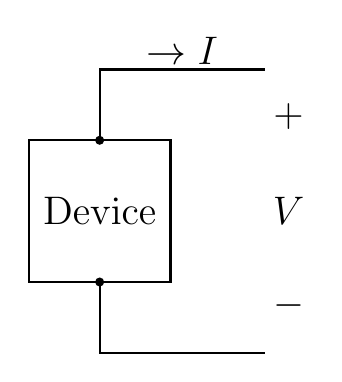
\begin{tikzpicture}[thick, scale=0.6]
    
    % Device Box
    \draw (0,0) rectangle (3, 3);
    \node at (1.5, 1.5) {\Large Device};
    
    % Top Terminal and Wire
    \filldraw (1.5, 3) circle (2pt);
    \draw (1.5, 3) -- (1.5, 4.5) -- (5, 4.5);
    \node at (3.25, 4.9) {\Large $\rightarrow I$};
    
    % Bottom Terminal and Wire
    \filldraw (1.5, 0) circle (2pt);
    \draw (1.5, 0) -- (1.5, -1.5) -- (5, -1.5);
    
    % Voltage Markings
    \node at (5.5, 3.5) {\Large $+$};
    \node at (5.5, 1.5) {\Large $V$};
    \node at (5.5, -0.5) {\Large $-$};


\end{tikzpicture}
\end{center}

\vspace{2cm}


 \mk{10} \yr{EEE 163 | L-1/T-1 | 2007--08}

\item Calculate the power delivered by the source $v_o$ using only source transformations if $I = 3/2$\,A in the circuit shown below.
\begin{center}
  
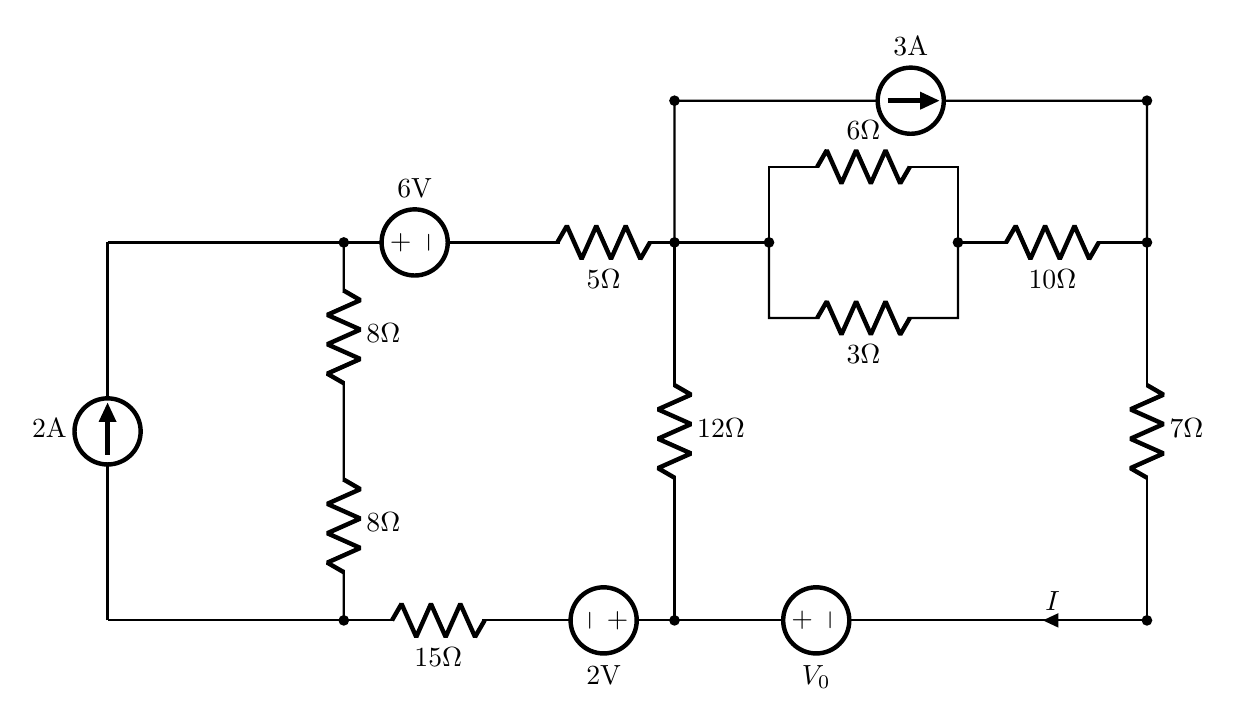
\begin{tikzpicture}[american, thick, x=1.2cm , y=1.2cm]

    % --- Left Loop ---
    % 2A Independent Current Source
    \draw (0,0) to[I, l=$2\text{A}$] (0,4);
    
    % Top and Bottom wires for the left loop
    \draw (0,4) -- (2.5,4);
    \draw (0,0) -- (2.5,0);
    
    % Vertical branch with two 8 Ohm resistors
    \draw (2.5,4) to[R, l=$8\Omega$] (2.5,2) 
                  to[R, l=$8\Omega$] (2.5,0);

    % --- Middle Section ---
    % Top branch: 6V Source, dashed wire, 5 Ohm resistor
    \draw (2.5,4) to[V, l=$6\text{V}$] (4,4);
    \draw (4,4) -- (4.5,4);
    \draw (4.5,4) to[R, l_=$5\Omega$] (6,4);
    
    % Bottom branch: 15 Ohm resistor, 2V Source
    \draw (2.5,0) to[R, l_=$15\Omega$] (4.5,0) 
                  to[V, invert, l_=$2\text{V}$] (6,0);
                  
    % Center vertical branch: 12 Ohm resistor
    \draw (6,4) to[R, l=$12\Omega$] (6,0);

    % --- Right Section ---
    % Top bypass branch: 3A Current Source
    \draw (6,4) -- (6, 5.5) to[I, l=$3\text{A}$] (11, 5.5) -- (11, 4);
    
    % Parallel Resistors Block (6 Ohm and 3 Ohm)
    \draw (6,4) -- (7,4);
    \draw (7,4) -- (7, 4.8) to[R, l=$6\Omega$] (9, 4.8) -- (9, 4);
    \draw (7,4) -- (7, 3.2) to[R, l_=$3\Omega$] (9, 3.2) -- (9, 4);
    
    % Series 10 Ohm Resistor
    \draw (9,4) to[R, l_=$10\Omega$] (11, 4);
    
    % Rightmost vertical branch: 7 Ohm Resistor
    \draw (11,4) to[R, l=$7\Omega$] (11,0);
    
    % Bottom branch: current label I and V0 Voltage Source
    \draw (11,0) to[short, i_=$I$] (9,0) 
                 to[V, invert, l=$V_0$] (6,0);

    % --- Junction Dots ---
    \filldraw (2.5,4) circle (1.5pt);
    \filldraw (2.5,0) circle (1.5pt);
    \filldraw (6,4) circle (1.5pt);
    \filldraw (6,0) circle (1.5pt);
    \filldraw (7,4) circle (1.5pt);
    \filldraw (9,4) circle (1.5pt);
    \filldraw (11,4) circle (1.5pt);
    \filldraw (11,0) circle (1.5pt);
    \filldraw (6,5.5) circle (1.5pt);
    \filldraw (11,5.5) circle (1.5pt);


\end{tikzpicture}
\end{center}
\mk{15} \yr{EEE 163 | L-1/T-1 | 2007--08}

\item Find the Th\'{e}venin equivalent circuit with respect to the terminals a--b for the circuit shown below.
\begin{center}
  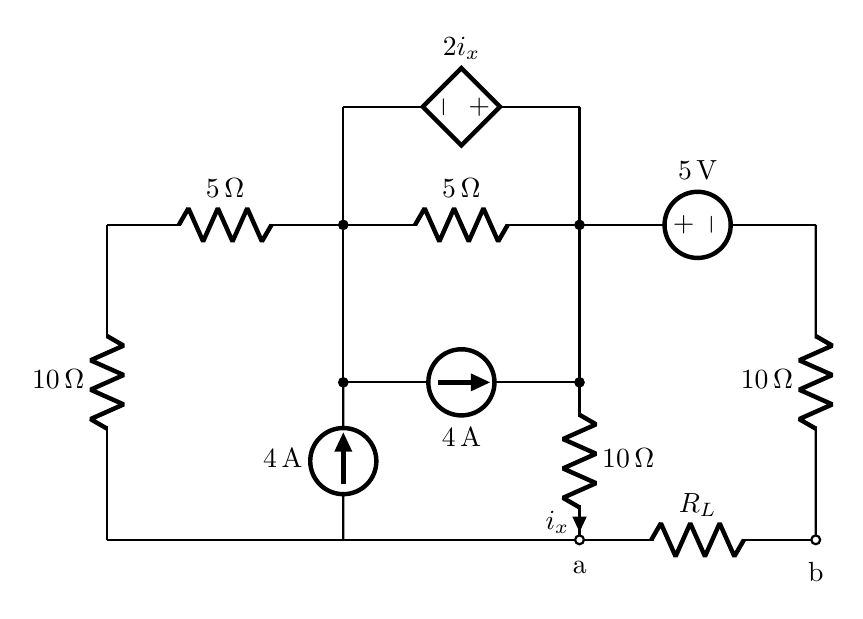
\begin{tikzpicture}[thick]

    % --- Bottom Return Wire ---
    \draw (0,0) -- (6,0);

    % --- Far-Left Branch ---
    \draw (0,0) to[R, l=$10\,\Omega$] (0,4);

    % --- Top-Left Horizontal Branch ---
    \draw (0,4) to[R, l=$5\,\Omega$] (3,4);

    % --- Middle-Left Vertical Branch ---
    \draw (3,0) to[I, l=$4\,\text{A}$] (3,2);
    \draw (3,2) -- (3,4);

    % --- Center Horizontal Branch (Current Source) ---
    \draw (3,2) to[I, l_=$4\,\text{A}$] (6,2);

    % --- Top-Middle Horizontal Branch (Resistor) ---
    \draw (3,4) to[R, l=$5\,\Omega$] (6,4);

    % --- Top Dependent Source Loop ---
    \draw (3,4) -- (3,5.5);
    \draw (6,4) -- (6,5.5);
    % Drawing right-to-left puts the '+' on the right and '-' on the left
    \draw (6,5.5) to[cV, l_=$2i_x$] (3,5.5); 

    % --- Middle-Right Vertical Branch ---
    \draw (6,4) -- (6,2);
    % i_ places the current label on the opposite side of the component
    \draw (6,2) to[R, l=$10\,\Omega$, i_=$i_x$] (6,0);

    % --- Far-Right Outer Branch ---
    \draw (6,4) to[V, l=$5\,\text{V}$] (9,4);
    \draw (9,4) to[R, l_=$10\,\Omega$] (9,0);

    % --- Bottom Right Load Resistor & Terminals ---
    % o-o creates the open terminal circles at nodes 'a' and 'b'
    \draw (6,0) to[R, l=$R_L$, o-o] (9,0);
    
    % Node Labels 'a' and 'b'
    \node[below] at (6, -0.15) {a};
    \node[below] at (9, -0.15) {b};

    % --- Connection Dots ---
    \filldraw (3,4) circle (1.5pt);
    \filldraw (6,4) circle (1.5pt);
    \filldraw (3,2) circle (1.5pt);
    \filldraw (6,2) circle (1.5pt);


\end{tikzpicture}
\end{center}
\mk{20} \yr{EEE 163 | L-1/T-1 | 2007--08}

\item Calculate $V$ using superposition principle for the circuit shown below.
\begin{center}
  \begin{circuitikz}[thick , transform shape, y=1.4cm]

    % Left branch: 4V Independent Voltage Source
    \draw (0,0) to [V,invert,  l=$4\text{ V}$] (0,2)
          to [short] (0,4);

    % Top branch: 5 ohm resistor and 2i_y dependent current source
    \draw (0,4) to [R, l=$5\ \Omega$, v_=$V$] (3,4);
    % Drawn right-to-left so the arrow points left
    \draw (6,4) to [cI, l_=$2i_y$] (3,4); 

    % Middle horizontal branch: 3v_x dependent voltage source
    \draw (0,2) to [cV,invert, l_=$3v_x$] (3,2);

    % Middle vertical branches: 10 ohm resistor and 3A source
    \draw (3,2) to [R, l=$10\ \Omega$, i_=$i_y$] (3,0);
    \draw (3,2) to [short] (5,2);
    % Drawn bottom-to-top so the arrow points up
    \draw (5,0) to [I, l_=$3\text{ A}$] (5,2); 

    % Rightmost branch (wire)
    \draw (6,4) to [short] (6,0);

    % Bottom branch: 5 ohm resistor and connecting wires
    % Drawn right-to-left to ensure the correct - v_x + polarity
    \draw (3,0) to [R, l_=$5\ \Omega$, v^=$v_x$] (0,0);
    \draw (3,0) to [short] (6,0);

    % Explicit junction dots for clarity
    \node[circ] at (0,2) {};
    \node[circ] at (3,2) {};
    \node[circ] at (3,0) {};
    \node[circ] at (5,0) {};

\end{circuitikz}
\end{center}
\mk{18} \yr{EEE 163 | L-1/T-1 | 2007--08}

\item If $I = 2.5$\,A, then find the value of $V_0$ using Source Transformation for the circuit shown below.
\begin{center}
  \begin{circuitikz}[thick]

    % ---------------------------------------------------
    % Leftmost Parallel Loop
    % ---------------------------------------------------
    % 2A current source pointing up
    \draw (0,0) to[I, l=$2\text{A}$] (0,3);
    \draw (0,3) -- (2,3);
    % 16 Ohm vertical resistor
    \draw (2,3) to[R, l=$16\,\Omega$] (2,0);
    \draw (2,0) -- (0,0);

    % ---------------------------------------------------
    % Middle-Left Connecting Branches
    % ---------------------------------------------------
    % 8V Voltage source (drawn left-to-right, + on left)
    \draw (2,3) to[V, l=$8\text{V}$] (4,3);
    % 20 Ohm horizontal resistor at the bottom
    \draw (2,0) to[R, l=$20\,\Omega$] (4,0);

    % ---------------------------------------------------
    % Central Vertical Branch
    % ---------------------------------------------------
    \draw (4,3) to[R, l=$12\,\Omega$] (4,0);

    % ---------------------------------------------------
    % Right Upper Multi-Bridge Branches
    % ---------------------------------------------------
    % Main line: 3 Ohm and 10 Ohm resistors
    \draw (4,3) to[R, l_=$3\,\Omega$] (7,3);
    \draw (7,3) to[R, l_=$10\,\Omega$] (10,3);

    % Middle bridge: 6 Ohm resistor
    \draw (4,3) -- (4,4.2)
          to[R, l=$6\,\Omega$] (7,4.2)
          -- (7,3);

    % Top bridge: 3A current source pointing right
    \draw (4,4.2) -- (4,5.4)
          to[I, l=$3\text{A}$] (10,5.4)
          -- (10,3);

    % ---------------------------------------------------
    % Far Right Vertical Branch
    % ---------------------------------------------------
    \draw (10,3) to[R, l=$7\,\Omega$] (10,0);

    % ---------------------------------------------------
    % Bottom Right Branch with V_0 and Current I
    % ---------------------------------------------------
    \draw (4,0) -- (6.5,0);
    % V_0 Source (drawn left-to-right, + on left)
    \draw (6.5,0) to[V, l=$V_0$] (8.5,0);
    % Wire with current I pointing left
    \draw (8.5,0) to[short, i_<=$I$] (10,0);

    % ---------------------------------------------------
    % Junction Nodes (Dots)
    % ---------------------------------------------------
    \node[circ] at (2,3) {};
    \node[circ] at (2,0) {};
    \node[circ] at (4,3) {};
    \node[circ] at (4,0) {};
    \node[circ] at (7,3) {};
    \node[circ] at (10,3) {};


\end{circuitikz}
\end{center}
\mk{15} \yr{EEE 163 | L-1/T-1 | 2006--07}

\item Find the voltage $v$ and the current $I$ using Th\'{e}venin's Theorem for the circuit shown below.
\begin{center}
  \begin{circuitikz}[thick]

    % ---------------------------------------------------
    % Left Vertical and Bottom Branches
    % ---------------------------------------------------
    \draw (0,4) -- (0,2);
    \draw (0,2) to[R, l=$4\,\Omega$] (0,0);
    \draw (0,0) to[R, l_=$3\,\Omega$] (3,0);

    % ---------------------------------------------------
    % Middle Horizontal Branches
    % ---------------------------------------------------
    \draw (0,2) to[R, l=$3\,\Omega$] (3,2);

    \draw (6,2) to[I, l_=$4\text{A}$] (3,2); 
    
    \draw (6,2) to[R, l=$5\,\Omega$] (8,2);

    % ---------------------------------------------------
    % Central Vertical Branches
    % ---------------------------------------------------
    \draw (3,2) to[R, l=$6\,\Omega$] (3,-1);
    
    % Bottom connection for the 3 Ohm resistor loop
    \draw (3,0) -- (8,0);
    \draw (3,-1) to[R, l_=$3\,\Omega$] (8,-1);
    \draw (8,0) -- (8,-1);

    % ---------------------------------------------------
    % Top Branch (Current I and Voltage V)
    % ---------------------------------------------------
    \draw (8,4) to[R, l_=$6\,\Omega$, v^>=$V$, i_>=$I$] (0,4); 
    % Note: I is pointing left, V has - on left, + on right.
    % circuitikz v^<= puts + on right, - on left. i_>= puts arrow pointing left.

    % ---------------------------------------------------
    % Right Vertical and Connecting Branches
    % ---------------------------------------------------
    \draw (8,2) -- (8,4);
    \draw (8,0) to[I, l_=$3\text{A}$] (8,2); % 3A pointing up
    
    % Far Right Loop
    \draw (8,2) to[R, l=$4\,\Omega$] (11,2);
    \draw (11,2) to[V, l=$10\text{V}$] (11,0); % + on top
    \draw (11,0) -- (8,0);

\end{circuitikz}
\end{center}
\mk{15} \yr{EEE 163 | L-1/T-1 | 2006--07}

\item Find the current $I$ using Superposition Theorem for the circuit shown below.
\begin{center}
  \begin{circuitikz}[thick, y=1.3cm]

    % ---------------------------------------------------
    % Leftmost Vertical Branch
    % ---------------------------------------------------
    % Drawn from bottom to top so standard labels appear on the left
    \draw (0,0) to[I, l=$6\text{A}$] (0,1.5) 
                to[R, l=$4\,\Omega$] (0,3);

    % ---------------------------------------------------
    % Top Horizontal Branch
    % ---------------------------------------------------
    \draw (0,3) -- (0,4.5);
    % Drawn right-to-left so the current arrow points left.
    % l_ places 6 Ohm above, l places 4A below the path.
    \draw (12,4.5) to[R, l_=$6\,\Omega$] (6,4.5) 
                   to[I, l=$4\text{A}$] (0,4.5);
    \draw (12,4.5) -- (12,3);

    % ---------------------------------------------------
    % Middle Horizontal Branches
    % ---------------------------------------------------
    \draw (0,3) to[R, l=$5\,\Omega$] (4,3);
    \draw (4,3) to[R, l=$4\,\Omega$] (8,3);
    \draw (8,3) to[R, l=$2\,\Omega$] (10,3) 
                to[V, l=$4\text{V}$] (12,3);

    % ---------------------------------------------------
    % Middle Vertical Branch (with Current I)
    % ---------------------------------------------------
    % Drawn top-to-bottom. i_ places the I label on the left, 
    % l places the component labels on the right.
    \draw (4,3) to[R, l=$2\,\Omega$, i=$I$] (4,1.5) 
                to[V, l=$10\text{V}$] (4,0);

    % ---------------------------------------------------
    % Second Middle Vertical Branch
    % ---------------------------------------------------
    % Drawn bottom-to-top. l_ places the label on the right.
    \draw (8,0) to[I, l_=$6\text{A}$] (8,3);

    \draw (12,3) to[R, l=$5\,\Omega$] (12,0);

    \draw (0,0) -- (12,0);


\end{circuitikz}
\end{center}
\mk{17} \yr{EEE 163 | L-1/T-1 | 2006--07}

\item Find the value of $R$ for which maximum power will be delivered to it. Also, find the value of the maximum power for the circuit shown below.
\begin{center}
  \begin{circuitikz}[thick]

    % ---------------------------------------------------
    % Left Vertical Branch (x = 0)
    % ---------------------------------------------------
    % 5V Source (+ on top). 
    \draw (0,6) to[V, l=$5\text{V}$] (0,3);
    
    % Resistor R and 20V Source (+ on top).
    \draw (0,3) to[R, l=$R$] (0,1.5) 
                to[V,invert,  l=$20\text{V}$] (0,0);

    % ---------------------------------------------------
    % Top Horizontal Branch (y = 6)
    % ---------------------------------------------------
    \draw (0,6) to[I, l=$6\text{A}$] (4,6) 
                to[R, l=$2\,\Omega$] (8,6) 
                -- (12,6);

    % ---------------------------------------------------
    % Middle Horizontal Branch (y = 3)
    % ---------------------------------------------------
    \draw (0,6) to[R, l=$2\,\Omega$] (4,3) 
                to[R, l=$6\,\Omega$] (8,3) 
                -- (12,3);

    % ---------------------------------------------------
    % Bottom Horizontal Branch (y = 0)
    % ---------------------------------------------------
    % 20 Ohm resistor and dashed line before the first junction
    \draw (0,0) -- (0.5,0) to[R, l=$20\,\Omega$] (4,0);


    % The correctly placed 5V source (- on left, + on right).
    % Drawn right-to-left so + is at the starting node (8,0).
    \draw (8,0) to[V, l_=$5\text{V}$] (4,0);

    % Plain wire connecting to the rightmost branch
    \draw (8,0) -- (12,0);

    % ---------------------------------------------------
    % Inner Vertical Branches
    % ---------------------------------------------------
    % 10 Ohm vertical branch (x = 4)
    \draw (4,3) to[R, l_=$10\,\Omega$] (4,0);
    
    % 4 Ohm vertical branch with the jump over the middle wire (x = 8)
    \draw (8,6) -- (8,3.15) arc (90:-90:0.15) 
                -- (8,2.5) to[R, l_=$4\,\Omega$] (8,0);

    % ---------------------------------------------------
    % Far Right Vertical Branch (x = 12)
    % ---------------------------------------------------
    % Top part (2 Ohm resistor)
    \draw (12,6) to[R, l_=$2\,\Omega$] (12,3);
    
    % Bottom part (3 Ohm resistor and 3A source pointing up)
    \draw (12,3) to[R, l_=$3\,\Omega$] (12,1.5);
    \draw (12,0) to[I, l_=$3\text{A}$] (12,1.5);

    % ---------------------------------------------------
    % Junction Nodes (Dots)
    % ---------------------------------------------------
    \node[circ] at (0,3) {};
    \node[circ] at (4,3) {};
    \node[circ] at (12,3) {};
    \node[circ] at (8,6) {};
    \node[circ] at (4,0) {};
    \node[circ] at (8,0) {};

\end{circuitikz}
\end{center}
\mk{18} \yr{EEE 163 | L-1/T-1 | 2006--07}

\item For the circuit shown below, find $I_1$ and $V_1$ using superposition theorem.
\begin{center}
  
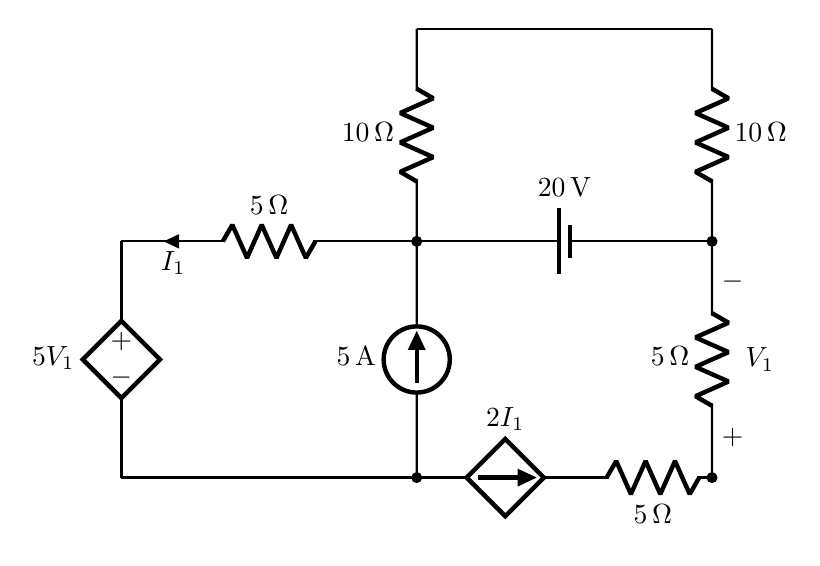
\begin{tikzpicture}[thick,x=1.5cm, y=1.5cm,>=stealth]

    % --- Leftmost Dependent Source ---
    % Drawn bottom-to-top so the positive (+) terminal is on top
    \draw (0,0) to[cV,invert,  l=$5V_1$] (0,2);
    
    % --- Top Left Horizontal Branch ---
    % Drawn right-to-left so the current arrow I1 points left
    \draw (2.5,2) to[R, l_=$5\,\Omega$, i=$I_1$] (0,2);
    
    % --- Bottom Left Wire ---
    \draw (0,0) -- (2.5,0);

    % --- Middle Vertical Column ---
    % Lower branch: 5A independent current source pointing UP
    \draw (2.5,0) to[I, l=$5\,\text{A}$] (2.5,2);
    % Upper branch: 10 Ohm resistor
    \draw (2.5,2) to[R, l=$10\,\Omega$] (2.5,3.8);

    % --- Middle Horizontal Branch ---
    % 20V battery: long plate on left, short on right
    \draw (2.5,2) to[battery1, l=$20\,\text{V}$] (5,2);

    % --- Right Vertical Column ---
    % Upper branch: 10 Ohm resistor
    \draw (5,2) to[R, l_=$10\,\Omega$] (5,3.8);
    % Lower branch: 5 Ohm resistor with V1 polarity (- on top, + on bottom)
    % Drawn bottom-to-top to place the '+' terminal at the bottom node
    \draw (5,0) to[R, l=$5\,\Omega$, v=$V_1$] (5,2);

    % --- Topmost Connecting Wire ---
    \draw (2.5,3.8) -- (5,3.8);

    % --- Bottom Right Horizontal Branch ---
    % Dependent current source 2I1 pointing right, in series with a 5 Ohm resistor
    \draw (2.5,0) to[cI, l=$2I_1$] (4,0)
                  to[R, l_=$5\,\Omega$] (5,0);

    % --- Connection Junction Dots ---
    \fill (2.5,2) circle (2pt);
    \fill (5,2) circle (2pt);
    \fill (2.5,0) circle (2pt);
    \fill (5,0) circle (2pt);


\end{tikzpicture}
\end{center}
\mk{18} \yr{EEE 163 | L-1/T-1 | 2005--06}

\item For the circuit shown below, find Th\'{e}venin's equivalent circuit between the terminals a--b.
\begin{center}
  
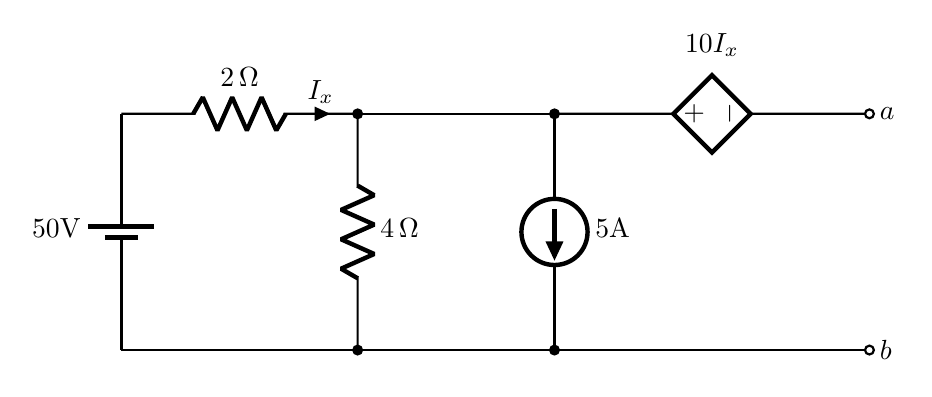
\begin{tikzpicture}[thick,>=stealth]

    % --- Leftmost Branch ---
    % 50V Battery: drawn bottom-to-top to place the positive (long) terminal at the top
    \draw (0,0) to[battery1,invert,  l=$50\text{V}$] (0,3);

    % --- Top Horizontal Branch (Left to Middle) ---
    % 2 Ohm resistor with current Ix flowing left-to-right
    \draw (0,3) to[R, l=$2\,\Omega$, i=$I_x$] (3,3);

    % --- First Middle Vertical Branch ---
    % 4 Ohm resistor drawn top-to-bottom
    \draw (3,3) to[R, l=$4\,\Omega$] (3,0);

    % --- Top Horizontal Connecting Wire (Middle) ---
    \draw (3,3) -- (5.5,3);

    % --- Second Middle Vertical Branch ---
    % 5A independent current source drawn top-to-bottom so the arrow points downwards
    \draw (5.5,3) to[I, l=$5\text{A}$] (5.5,0);

    % --- Top Right Branch (Dependent Source and Terminal 'a') ---
    % Dependent voltage source 10Ix. 
    % Drawn left-to-right. Using v=... explicitly shows the +/- polarity (+ on left).
    \draw (5.5,3) -- (6.5,3) 
                  to[cV, v=$10I_x$] (8.5,3) 
                  to[short, -o] (9.5,3) node[right] {$a$};

    % --- Bottom Common Ground/Return Wire and Terminal 'b' ---
    \draw (0,0) -- (8.5,0) to[short, -o] (9.5,0) node[right] {$b$};

    % --- Junction Dots ---
    \fill (3,3) circle (2pt);
    \fill (3,0) circle (2pt);
    \fill (5.5,3) circle (2pt);
    \fill (5.5,0) circle (2pt);

\end{tikzpicture}
\end{center}
\mk{17} \yr{EEE 163 | L-1/T-1 | 2005--06}

\item For the circuit shown below, find Norton's equivalent circuit between the terminals a--b.
\begin{center}
  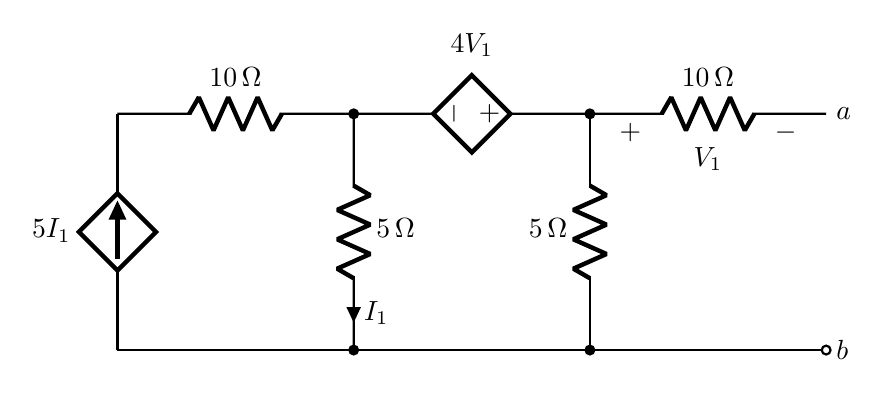
\begin{tikzpicture}[thick, >=stealth]

    % --- Leftmost Branch ---
    % Dependent current source 5I1 pointing UP
    \draw (0,0) to[cI, l=$5I_1$] (0,3);

    % --- Top Left Horizontal Branch ---
    % 10 Ohm resistor
    \draw (0,3) to[R, l=$10\,\Omega$] (3,3);

    % --- Middle Vertical Branch ---
    % 5 Ohm resistor with current I1 flowing DOWN
    \draw (3,3) to[R, l=$5\,\Omega$, i=$I_1$] (3,0);

    % --- Top Middle Horizontal Branch ---
    % Dependent voltage source 4V1 with '+' on the right
    \draw (3,3) to[cV,invert, v=$4V_1$] (6,3);

    % --- Right Vertical Branch ---
    % 5 Ohm resistor
    \draw (6,3) to[R, l_=$5\,\Omega$] (6,0);

    % --- Top Right Horizontal Branch (to terminal 'a') ---
    % 10 Ohm resistor with voltage V1 polarity (- on left, + on right)
    \draw (6,3) to[R, l=$10\,\Omega$, v=$V_1$] (9,3) node[right] {$a$};
    % --- Bottom Common Return (to terminal 'b') ---
    \draw (0,0) -- (6,0) 
    (6,0) to[short, -o] (9,0) node[right] {$b$};

    % --- Junction Dots ---
    \fill (3,3) circle (2pt);
    \fill (3,0) circle (2pt);
    \fill (6,3) circle (2pt);
    \fill (6,0) circle (2pt);



\end{tikzpicture}
\end{center}
\mk{18} \yr{EEE 163 | L-1/T-1 | 2005--06}

\item Find the value of load resistance $R_L$ for maximum power transfer to the load for the circuit shown below. What is that maximum power?
\begin{center}
  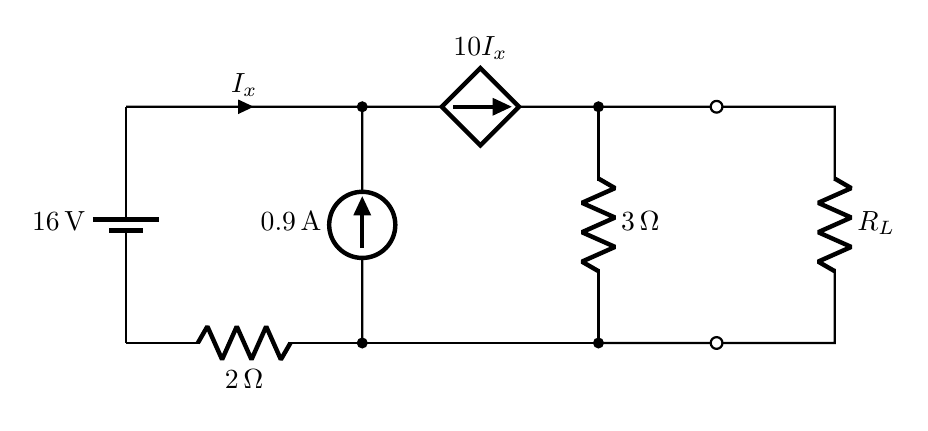
\begin{tikzpicture}[thick,>=stealth]

    % --- Leftmost Vertical Branch ---
    % 16V Battery: long bar on top, short on bottom
    \draw (0,0) to[battery1,invert,  l=$16\,\text{V}$] (0,3);

    % --- Top Left Horizontal Wire ---
    % Current Ix flowing from left to right
    \draw (0,3) to[short, i=$I_x$] (3,3);

    % --- Bottom Left Horizontal Branch ---
    % 2 Ohm resistor placed on the bottom wire
    \draw (0,0) to[R, l_=$2\,\Omega$] (3,0);

    % --- First Middle Vertical Branch ---
    % 0.9A independent current source pointing UP
    \draw (3,0) to[I, l=$0.9\,\text{A}$] (3,3);

    % --- Top Middle Horizontal Branch ---
    % Dependent current source 10Ix pointing right
    \draw (3,3) to[cI, l=$10I_x$] (6,3);

    % --- Bottom Middle Connecting Wire ---
    \draw (3,0) -- (6,0);

    % --- Second Middle Vertical Branch ---
    % 3 Ohm resistor
    \draw (6,3) to[R, l=$3\,\Omega$] (6,0);

    % --- Right Terminals and Load Resistor (RL) ---
    % Drawing the lines, the open terminal circles, and the load resistor RL
    \draw (6,3) -- (7.5,3) node[circle, draw, fill=white, inner sep=1.5pt] {} -- (9,3)
                to[R, l=$R_L$] (9,0)
                -- (7.5,0) node[circle, draw, fill=white, inner sep=1.5pt] {} -- (6,0);

    % --- Junction Dots ---
    \fill (3,3) circle (2pt);
    \fill (3,0) circle (2pt);
    \fill (6,3) circle (2pt);
    \fill (6,0) circle (2pt);


\end{tikzpicture}

\end{center}
\mk{17} \yr{EEE 163 | L-1/T-1 | 2005--06}

\end{enumerate}


%% ══════════════════════════════════════════════════════════════════════
%%  PART II
%% ══════════════════════════════════════════════════════════════════════
\secdivider{Part II --- Alternating Current (AC) Circuits}{RMS \& Average Values, Sinusoids, Phasors, RL/RC/RLC Analysis, Power}{cB}

%% ══════════════════════════════════════════════════════════════════════
%%  SECTION 2: AC FUNDAMENTALS & RLC CIRCUITS
%% ══════════════════════════════════════════════════════════════════════
\markboth{S2: AC Fundamentals \& RLC Circuits}{S2: AC Fundamentals \& RLC Circuits}
\label{sec:S2}
\titleformat{\section}{\large\bfseries\color{cB}}{}{0em}{}[\titlerule]
\section*{S2 \quad AC Fundamentals \& RLC Circuits}
\addcontentsline{toc}{section}{S2: AC Fundamentals \& RLC Circuits}

%%──────────────────────────────────────────────────────────────────────
\subtopic{cB}{RMS \& Average Values}
\label{sub:s2-rms}

\begin{enumerate}


\item Find the effective(RMS) and average values of the voltage, V shown in the figure below.

\begin{center}
      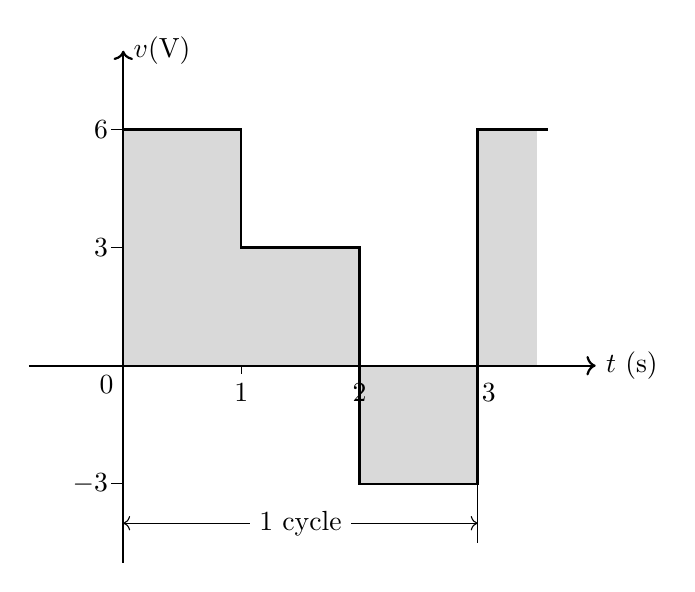
\begin{tikzpicture}[xscale=1.5, yscale=0.5]
        
        % Shaded regions
        \fill[gray!30] (0,0) rectangle (1,6);
        \fill[gray!30] (1,0) rectangle (2,3);
        \fill[gray!30] (2,0) rectangle (3,-3);
        \fill[gray!30] (3,0) rectangle (3.5,6);

        % Axes
        \draw[->, thick] (-0.8,0) -- (4,0) node[right] {$t\ (\mathrm{s})$};
        \draw[->, thick] (0,-5) -- (0,8) node[right] {$v(\mathrm{V})$};

        % Y-axis ticks and labels
        \draw (-0.1,6) -- (0,6) node[left=2pt] {$6$};
        \draw (-0.1,3) -- (0,3) node[left=2pt] {$3$};
        \draw (-0.1,-3) -- (0,-3) node[left=2pt] {$-3$};
        \node[below left] at (0,0) {$0$};

        % X-axis ticks and labels
        \draw (1,0) -- (1,-0.2) node[below] {$1$};
        \draw (2,0) -- (2,-0.2) node[below] {$2$};
        % Shifted '3' slightly right to avoid overlapping the line
        \draw (3,0) -- (3,-0.2) node[below right, xshift=-2pt] {$3$}; 

        % Waveform outline (drawn after shading so it stays on top)
        \draw[thick] (0,6) -- (1,6) -- (1,3) -- (2,3) -- (2,-3) -- (3,-3) -- (3,6) -- (3.6,6);

        % "1 cycle" dimension line
        % Extending the y-axis down for the left bound
        \draw (0,-3) -- (0,-4.5);
        % Extending a line from t=3 for the right bound
        \draw (3,-3) -- (3,-4.5);
        % The dimension arrow
        \draw[<->] (0,-4) -- (3,-4) node[midway, fill=white] {1 cycle};

    \end{tikzpicture}

\end{center}

\mk{10} \yr{EEE 163 | L-1/T-1 | 2024--25}

  \item Find the effective (RMS) and average values of the voltage $v$ shown below .
\begin{center}
  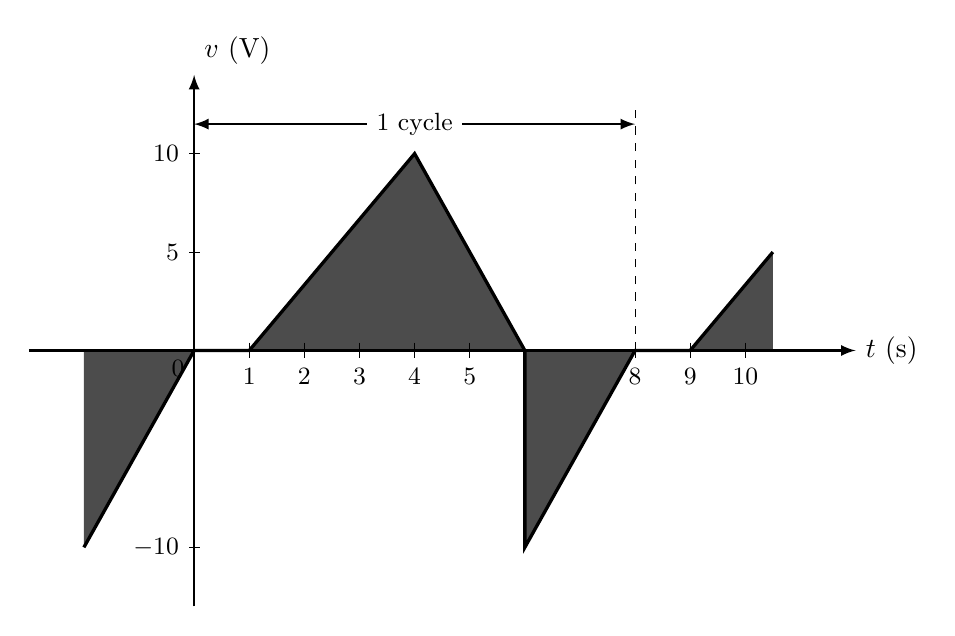
\begin{tikzpicture}[x=0.7cm, y=0.25cm, >=latex]

    % Shading/Filling the areas under the curve
    % Previous cycle (left of Y-axis)
    \fill[black!70] (0,0) -- (-2,-10) -- (-2,0) -- cycle;
    
    % Positive half cycle (from t=1 to t=6)
    \fill[black!70] (1,0) -- (4,10) -- (6,0) -- cycle;
    
    % Negative half cycle (from t=6 to t=8)
    \fill[black!70] (6,0) -- (6,-10) -- (8,0) -- cycle;
    
    % Next cycle start (from t=9 to t=10.5)
    \fill[black!70] (9,0) -- (10.5,5) -- (10.5,0) -- cycle;

    % Draw Axes
    \draw[->, thick] (-3,0) -- (12,0) node[right] {$t\text{ (s)}$};
    \draw[->, thick] (0,-13) -- (0,14) node[above right] {$v\text{ (V)}$};

    % Draw the actual Waveform Lines
    \draw[very thick] (-2,-10) -- (0,0) -- (1,0) -- (4,10) -- (6,0);
    \draw[very thick] (6,0) -- (6,-10) -- (8,0) -- (9,0) -- (10.5,5);

    % X-axis Ticks and Labels (1, 2, 3, 4, 5, 8, 9, 10)
    \foreach \x in {1,2,3,4,5,8,9,10} {
        \draw (\x,0.4) -- (\x,-0.4) node[below] {\small $\x$};
    }
    \node[below left] at (0,0) {\small $0$};

    % Y-axis Ticks and Labels (10, 5, -10)
    \draw (0.1,10) -- (-0.1,10) node[left] {\small $10$};
    \draw (0.1,5) -- (-0.1,5) node[left] {\small $5$};
    \draw (0.1,-10) -- (-0.1,-10) node[left] {\small $-10$};

    % "1 cycle" indicator extension lines and double-arrow
    \draw[dashed, thin] (0,0) -- (0,12.5);
    \draw[dashed, thin] (8,0) -- (8,12.5);
    \draw[<->, thick] (0,11.5) -- (8,11.5) node[midway, fill=white] {\small 1 cycle};

\end{tikzpicture}
\end{center}
\mk{15} \yr{EEE 163 | L-1/T-1 | 2023--24, 2011--12}

\item Find the RMS and average values of the signal shown in the Figure.
\begin{center}
  
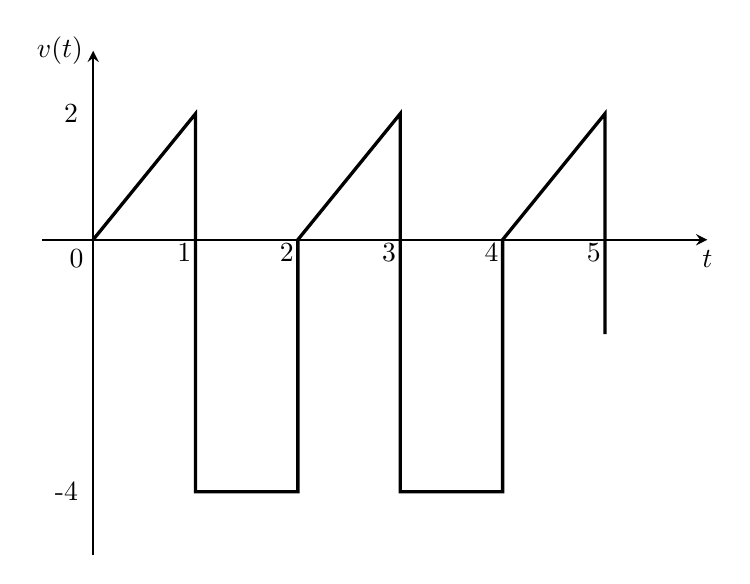
\begin{tikzpicture}[x=1.3cm, y=0.8cm, >=stealth]
    % Draw Axes
    \draw[->, thick] (-0.5, 0) -- (6.0, 0) node[below] {$t$};
    \draw[->, thick] (0, -5.0) -- (0, 3.0) node[left] {$v(t)$};
    
    % Plot the periodic waveform
    \draw[line width=1.2pt] (0,0) 
        -- (1,2) 
        -- (1,-4) 
        -- (2,-4) 
        -- (2,0)
        -- (3,2) 
        -- (3,-4) 
        -- (4,-4) 
        -- (4,0)
        -- (5,2) 
        -- (5,-1.5); % Terminating mid-drop as shown in the figure
        
    % Y-axis labels
    \node[left, xshift=-2pt] at (0,2) {2};
    \node[left, xshift=-2pt] at (0,-4) {-4};
    \node[below left] at (0,0) {0};
    
    % X-axis labels (offset slightly to match the original style)
    \node[below left, xshift=2pt, yshift=2pt] at (1,0) {1};
    \node[below left, xshift=2pt, yshift=2pt] at (2,0) {2};
    \node[below left, xshift=2pt, yshift=2pt] at (3,0) {3};
    \node[below left, xshift=2pt, yshift=2pt] at (4,0) {4};
    \node[below left, xshift=2pt, yshift=2pt] at (5,0) {5};
    
\end{tikzpicture}

\end{center}
\mk{12} \yr{EEE 163 | L-1/T-1 | 2022--23}

\item Calculate the effective value of the current waveform shown below and the average power delivered to a 12\,$\Omega$ resistor when the current runs through the resistor.
\begin{center}
  \begin{tikzpicture}
\begin{axis}[
    % Axis styling
    axis lines=middle,
    xlabel={$t$ (sec)},
    ylabel={$i(t)$ A},
    xmin=-0.5, xmax=5.8,
    ymin=-1, ymax=13,
    % Fine-tuning label placement
    xlabel style={at={(current axis.right of origin)}, anchor=west, xshift=2mm},
    ylabel style={at={(current axis.above origin)}, anchor=east, yshift=2mm},
    % Setting exact tick marks matching the drawing
    xtick={0, 1, 2, 3, 4, 5},
    ytick={10},
    xticklabel style={anchor=north},
    yticklabel style={anchor=east},
    % Curve styling
    every axis plot/.append style={line width=1.2pt, color=black}
]

    % --- FIRST PERIOD (0 to 3) ---
    % Constant flat top from 0 to 1
    \addplot[domain=0:1] {10};
    
    % Linear ramp down from 1 to 2
    \addplot[domain=1:2] {10 - 10*(x-1)};
    
    % Dead period/flat line at zero from 2 to 3
    \addplot[domain=2:3] {0};

    % --- SECOND PERIOD (3 to 5.5) ---
    % Vertical jump up at t = 3
    \draw[line width=1.2pt] (axis cs:3,0) -- (axis cs:3,10);
    
    % Constant flat top from 3 to 4
    \addplot[domain=3:4] {10};
    
    % Linear ramp down from 4 to 5
    \addplot[domain=4:5] {10 - 10*(x-4)};
    
    % Post-pulse flat line at zero from 5 onwards
    \addplot[domain=5:5.5] {0};

\end{axis}
\end{tikzpicture}

\end{center}
\mk{17} \yr{EEE 163 | L-1/T-1 | 2020--21}

\item Find the rms value of the waveforms belowb.
\begin{center}
  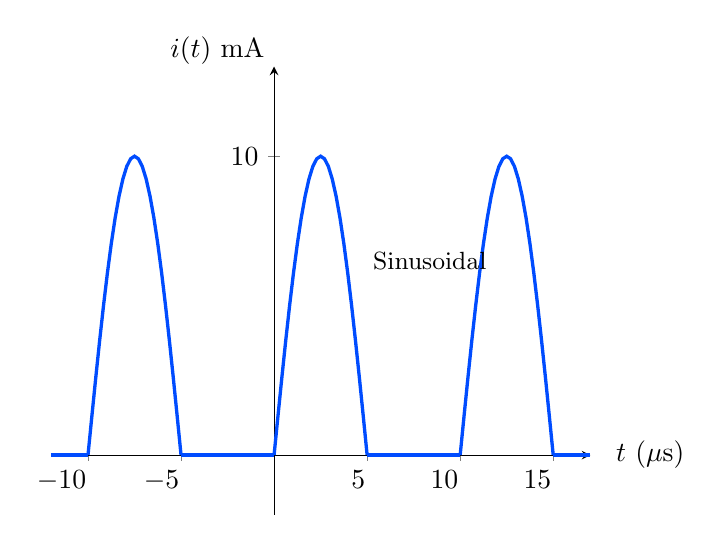
\begin{tikzpicture}
\begin{axis}[
    axis lines=middle,
    xlabel={$t$ ($\mu$s)},
    ylabel={$i(t)$ mA},
    xmin=-12, xmax=17, % Extended xmin to cleanly show the -10 region
    ymin=-2, ymax=13,
    xlabel style={at={(current axis.right of origin)}, anchor=west, xshift=2mm},
    ylabel style={at={(current axis.above origin)}, anchor=east, yshift=2mm},
    % Added -10 to the explicit tick marks
    xtick={-10, -5, 0, 5, 10, 15},
    ytick={10},
    xticklabel style={anchor=north east, xshift=1mm},
    yticklabel style={anchor=east},
    every axis plot/.append style={line width=1.2pt, color=blue!70!cyan}
]

    % Trailing flat line before -10
    \addplot[domain=-12:-10] {0};

    % CORRECTED: Sinusoidal pulse from -10 to -5
    \addplot[domain=-10:-5] {10*sin(deg(pi*(x+10)/5))};
    
    % Flat line from -5 to 0
    \addplot[domain=-5:0] {0};

    % Sinusoidal pulse from 0 to 5
    \addplot[domain=0:5] {10*sin(deg(pi*x/5))};

    % Flat line from 5 to 10
    \addplot[domain=5:10] {0};

    % Sinusoidal pulse from 10 to 15
    \addplot[domain=10:15] {10*sin(deg(pi*(x-10)/5))};

    % Trailing flat line after 15
    \addplot[domain=15:17] {0};

    % Text label placement
    \node[anchor=west, font=\small] at (axis cs:4.8,6.5) {Sinusoidal};

\end{axis}
\end{tikzpicture}

\end{center}
\mk{10} \yr{EEE 163 | L-1/T-1 | 2018--19}

\item Find the r.m.s.\ value of the voltage having the wave shape as shown below.
\begin{center}
  \begin{tikzpicture}
\begin{axis}[
    width=14cm, height=7cm,
    axis x line=middle,
    axis y line=left,
    xlabel={$\omega t$ (rad.)},
    ylabel={$V$ (volts)},
    xlabel style={at={(ticklabel* cs:1)}, anchor=west},
    ylabel style={at={(ticklabel* cs:1)}, anchor=south},
    xmin=0, xmax=9.5,
    ymin=-18, ymax=18,
    xtick={
        0.7854, 1.5708, 2.3562, 3.1416, 3.9270, 
        4.7124, 5.4978, 6.2832, 7.0686, 7.8540, 8.6394
    },
    xticklabels={
        $\frac{\pi}{4}$, $\frac{\pi}{2}$, $\frac{3\pi}{4}$, $\pi$, $\frac{5\pi}{4}$, 
        $\frac{3\pi}{2}$, $\frac{7\pi}{4}$, $2\pi$, $\frac{9\pi}{4}$, $\frac{5\pi}{2}$, $\frac{11\pi}{4}$
    },
    ytick={-15, 0, 10, 15},
    yticklabels={$-15$, $0$, $10$, $15$},
    tick label style={font=\small},
    every axis x label/.style={at={(current axis.right of origin)},anchor=west, xshift=5pt},
    every axis y label/.style={at={(current axis.above origin)},anchor=south, yshift=5pt},
    clip=false
]

    % --- Dashed Reference Lines ---
    \draw[dashed, thin, gray] (axis cs:0,15) -- (axis cs:6.2832,15);
    \draw[dashed, thin, gray] (axis cs:0,10) -- (axis cs:4.7124,10);
    \draw[dashed, thin, gray] (axis cs:0,-15) -- (axis cs:3.1416,-15);

    % --- Waveform Segments ---
    % 1. From 0 to pi/4
    \addplot[thick, domain=0:pi/4] {0};
    
    % Vertical jump at pi/4
    \draw[thick] (axis cs:pi/4, 0) -- (axis cs:pi/4, 15);
    
    % 2. Linear decay from pi/4 to pi/2
    \addplot[thick, domain=pi/4:pi/2] {15 - (60/pi)*(x - pi/4)};
    
    % 3. Sinusoidal wave from pi/2 to 3*pi/2
    \addplot[thick, domain=pi/2:3*pi/2, samples=100] {15*cos(deg(x))};
    
    % Vertical jump at 3*pi/2
    \draw[thick] (axis cs:3*pi/2, 0) -- (axis cs:3*pi/2, 10);
    
    % 4. Constant flat line from 3*pi/2 to 7*pi/4
    \addplot[thick, domain=3*pi/2:7*pi/4] {10};
    
    % 5. Linear rise from 7*pi/4 to 2*pi
    \addplot[thick, domain=7*pi/4:2*pi] {10 + (20/pi)*(x - 7*pi/4)};
    
    % Vertical drop at 2*pi
    \draw[thick] (axis cs:2*pi, 15) -- (axis cs:2*pi, 0);
    
    % 6. Flat line at 0 from 2*pi to 9*pi/4
    \addplot[thick, domain=2*pi:9*pi/4] {0};
    
    % Vertical jump at 9*pi/4
    \draw[thick] (axis cs:9*pi/4, 0) -- (axis cs:9*pi/4, 15);
    
    % 7. Linear decay from 9*pi/4 to 5*pi/2
    \addplot[thick, domain=9*pi/4:5*pi/2] {15 - (60/pi)*(x - 9*pi/4)};
    
    % 8. Continuing sinusoidal curve past 5*pi/2 to 11*pi/4
    \addplot[thick, domain=5*pi/2:11*pi/4, samples=50] {15*cos(deg(x))};

    % --- Annotations ---
    % Arrow pointing to the sinusoidal part
    \node (sine_text) at (axis cs:5.2, -12) [align=center, font=\small] {Sinusoidal\\wave};
    \draw[->, >=stealth, semithick] (sine_text.west) to [bend left=15] (axis cs:4.0, -10);

    % Dots on key axis intercepts for clarity
    \fill (axis cs:pi/4,0) circle (1.5pt);
    \fill (axis cs:pi/2,0) circle (1.5pt);
    \fill (axis cs:3*pi/2,0) circle (1.5pt);
    \fill (axis cs:5*pi/2,0) circle (1.5pt);
    \fill (axis cs:11*pi/4,0) circle (1.5pt);

\end{axis}

\end{tikzpicture}
\end{center}
\mk{20} \yr{EEE 163 | L-1/T-1 | 2014--15}

\item Determine the rms value for the waveform $f(t)$ given below.
\begin{center}
  \begin{tikzpicture}
    \begin{axis}[
        axis lines=left,
        xmin=0, xmax=9,
        ymin=0, ymax=9.5,
        xlabel={$t$},
        ylabel={$f(t)$},
        xtick={1,2,3,4,5,6,7,8},
        ytick={2,4,6,8},
        % Explicitly add 0 to the origin to match the drawing
        extra x ticks={0},
        extra x tick style={tick label style={anchor=north east}},
        every axis x label/.style={at={(ticklabel* cs:1)}, anchor=west},
        every axis y label/.style={at={(ticklabel* cs:1)}, anchor=south},
        clip=false % Allow drawing outside the main axis box
    ]
    
    % The periodic trapezoidal waveform
    \addplot[thick, mark=none] coordinates {
        (0,0) (2,4) (3,4) (4,0) (6,4) (7,4) (8,0)
    };

    % Vertical boundary lines for the "1 cycle" marker
    \draw (0, 0) -- (0, -1.2);
    \draw (4, 0) -- (4, -1.2);
    
    % "1 cycle" double-headed arrow and label
    \draw[<->] (0, -0.9) -- (4, -0.9) node[midway, below] {1 cycle};
    
    \end{axis}
\end{tikzpicture}

\end{center}
\mk{17} \yr{EEE 163 | L-1/T-1 | 2013--14}

\item Find the average and rms values of the current wave shown below.
\begin{center}
  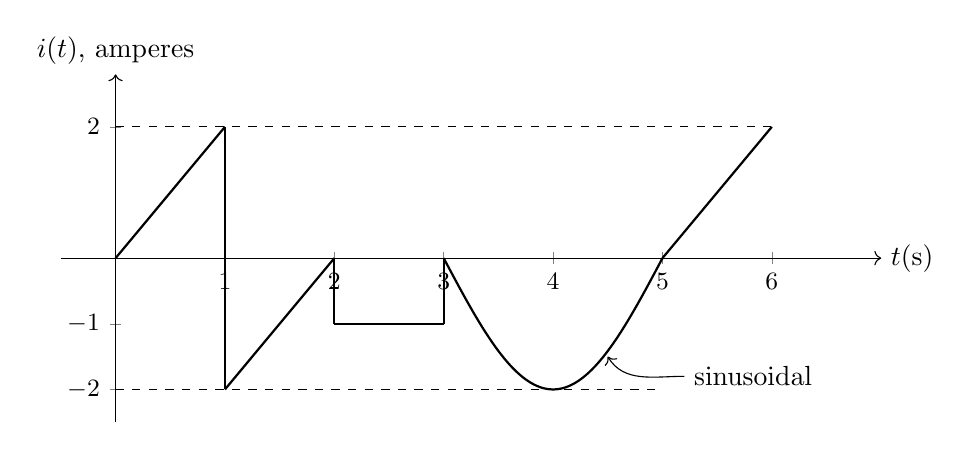
\begin{tikzpicture}
    \begin{axis}[
        axis lines=middle,
        xlabel={$t(\text{s})$},
        ylabel={$i(t)\text{, amperes}$},
        xmin=-0.5, xmax=7,
        ymin=-2.5, ymax=2.8,
        xtick={1, 2, 3, 4, 5, 6},
        ytick={-2, -1, 2},
        every axis x label/.style={at={(ticklabel* cs:1.0)}, anchor=west},
        every axis y label/.style={at={(ticklabel* cs:1.0)}, anchor=south},
        axis line style={->},
        tick label style={font=\small},
        width=12cm,
        height=6cm,
        % Remove minor ticks and grids to match the hand-drawn style
        grid=none
    ]
    
    % Dashed horizontal guide lines
    \draw[dashed] (axis cs:0,2) -- (axis cs:6,2);
    \draw[dashed] (axis cs:0,-2) -- (axis cs:5,-2);
    
    % Piecewise linear waveform segments
    % 1. Line from origin to (1,2)
    \draw[thick] (axis cs:0,0) -- (axis cs:1,2);
    
    % 2. Vertical drop at t=1
    \draw[thick] (axis cs:1,2) -- (axis cs:1,-2);
    
    % 3. Line from (1,-2) to (2,0)
    \draw[thick] (axis cs:1,-2) -- (axis cs:2,0);
    
    % 4. Vertical drop at t=2
    \draw[thick] (axis cs:2,0) -- (axis cs:2,-1);
    
    % 5. Horizontal line from t=2 to t=3
    \draw[thick] (axis cs:2,-1) -- (axis cs:3,-1);
    
    % 6. Vertical jump at t=3
    \draw[thick] (axis cs:3,-1) -- (axis cs:3,0);
    
    % 7. Sinusoidal curve from t=3 to t=5
    \addplot[thick, domain=3:5, samples=100] {-2*sin(deg(pi*(x-3)/2))};
    
    % 8. Final straight line from t=5 to t=6
    \draw[thick] (axis cs:5,0) -- (axis cs:6,2);
    
    % Annotations
    \draw[<-] (axis cs:4.5,-1.5) to[out=-60,in=180] (axis cs:5.2,-1.8) node[right] {sinusoidal};
    
    \end{axis}
\end{tikzpicture}

\end{center}
\mk{25} \yr{EEE 163 | L-1/T-1 | 2012--13}

\item The voltage waveform shown below is a periodic signal. Determine the crest factor of the waveform.
\begin{center}
  \begin{center}
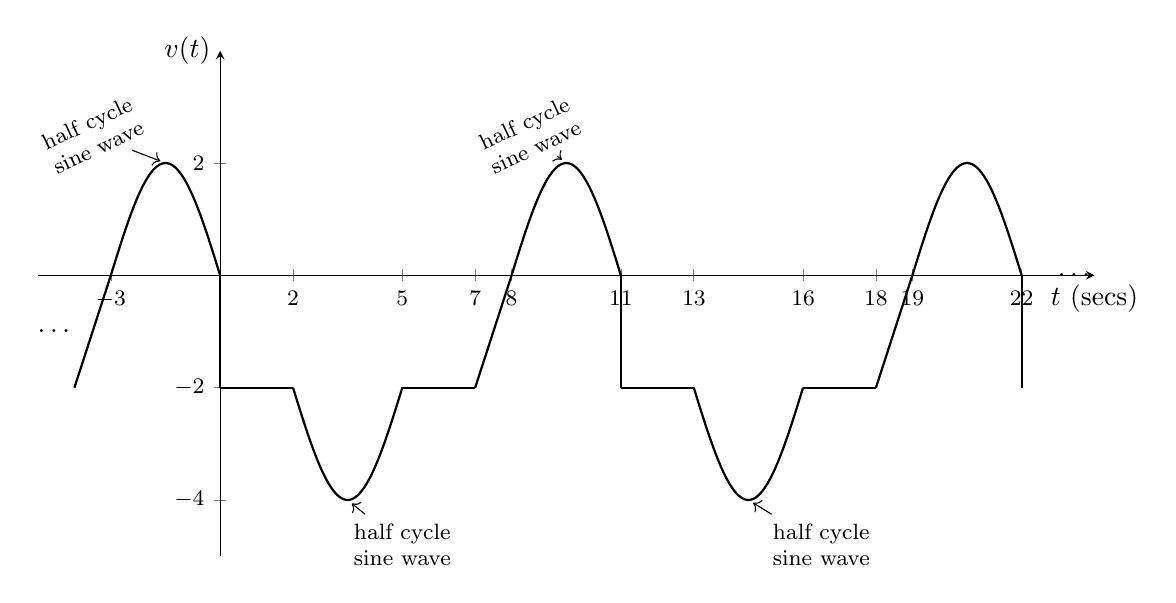
\begin{tikzpicture}
\begin{axis}[
    width=15cm,
    height=8cm,
    axis lines=middle,
    xmin=-5, xmax=24,
    ymin=-5, ymax=4,
    xlabel={$t\text{ (secs)}$},
    ylabel={$v(t)$},
    xlabel style={anchor=north},
    ylabel style={anchor=east},
    xtick={-3, 2, 5, 7, 8, 11, 13, 16, 18, 19, 22},
    ytick={-4, -2, 2},
    tick label style={font=\footnotesize},
    enlargelimits=false,
    clip=false
]

% Cycle 0 (Partial, ending at t=0)
\addplot[domain=-4:-3, thick, samples=2] {2*(x+4)-2};
\addplot[domain=-3:0, thick, samples=50] {2*sin(deg(pi*(x+3)/3))};
\draw[thick] (axis cs:0,0) -- (axis cs:0,-2);

% Cycle 1 (t=0 to t=11)
\addplot[domain=0:2, thick, samples=2] {-2};
\addplot[domain=2:5, thick, samples=50] {-2 - 2*sin(deg(pi*(x-2)/3))};
\addplot[domain=5:7, thick, samples=2] {-2};
\addplot[domain=7:8, thick, samples=2] {2*(x-7)-2};
\addplot[domain=8:11, thick, samples=50] {2*sin(deg(pi*(x-8)/3))};
\draw[thick] (axis cs:11,0) -- (axis cs:11,-2);

% Cycle 2 (t=11 to t=22)
\addplot[domain=11:13, thick, samples=2] {-2};
\addplot[domain=13:16, thick, samples=50] {-2 - 2*sin(deg(pi*(x-13)/3))};
\addplot[domain=16:18, thick, samples=2] {-2};
\addplot[domain=18:19, thick, samples=2] {2*(x-18)-2};
\addplot[domain=19:22, thick, samples=50] {2*sin(deg(pi*(x-19)/3))};
\draw[thick] (axis cs:22,0) -- (axis cs:22,-2); 

% Annotations pointing to the sine waves
\node[align=center, rotate=25, font=\footnotesize] (a1) at (axis cs:-3.5, 2.5) {half cycle \\ sine wave};
\draw[->, shorten >=2pt] (a1) -- (axis cs:-1.5, 2);

\node[align=center, font=\footnotesize] (a2) at (axis cs:5, -4.8) {half cycle \\ sine wave};
\draw[->, shorten >=2pt] (a2) -- (axis cs:3.5, -4);

\node[align=center, rotate=25, font=\footnotesize] (a3) at (axis cs:8.5, 2.5) {half cycle \\ sine wave};
\draw[->, shorten >=2pt] (a3) -- (axis cs:9.5, 2);

\node[align=center, font=\footnotesize] (a4) at (axis cs:16.5, -4.8) {half cycle \\ sine wave};
\draw[->, shorten >=2pt] (a4) -- (axis cs:14.5, -4);

% Dotted continuations indicating periodicity
\node at (axis cs:-4.5, -1) {\dots};
\node at (axis cs:23.5, 0) {\dots};

\end{axis}
\end{tikzpicture}
\end{center}
\end{center}
\mk{20} \yr{EEE 163 | L-1/T-1 | 2007--08}

\item Calculate the effective voltage across the resistance for the circuit shown below.

\begin{center}
\begin{circuitikz}[thick,scale=1.2, transform shape]
    % Draw the main circuit loop
    \draw (0,0)
        % AC Voltage Source
        to[sV, name=Vs] (0,3)
        % Inductor
        to[L, l=$0.05\text{ H}$] (3,3)
        % Capacitor
        to[C, l=$100\,\mu\text{F}$] (6,3)
        % Resistor (label on the outside/right)
        to[R, l=$8\,\Omega$] (6,0)
        % Bottom wire closing the loop
        to[short] (0,0);

    % Multiline label for the AC voltage source
    % Placed to the right of the source to match the image
    \node[anchor=west, align=left] at (Vs.east) {
        $v$ \\
        $= 8 \sin(100\pi t + 30^\circ)$ \\
        $\quad + 6 \cos(100\pi t + 30^\circ)$
    };


\end{circuitikz}
\end{center}
\mk{10} \yr{EEE 163 | L-1/T-1 | 2007--08}

\item The voltage waveshape shown below is a periodic signal. Determine the crest factor of the given periodic signal.
\begin{center}
  
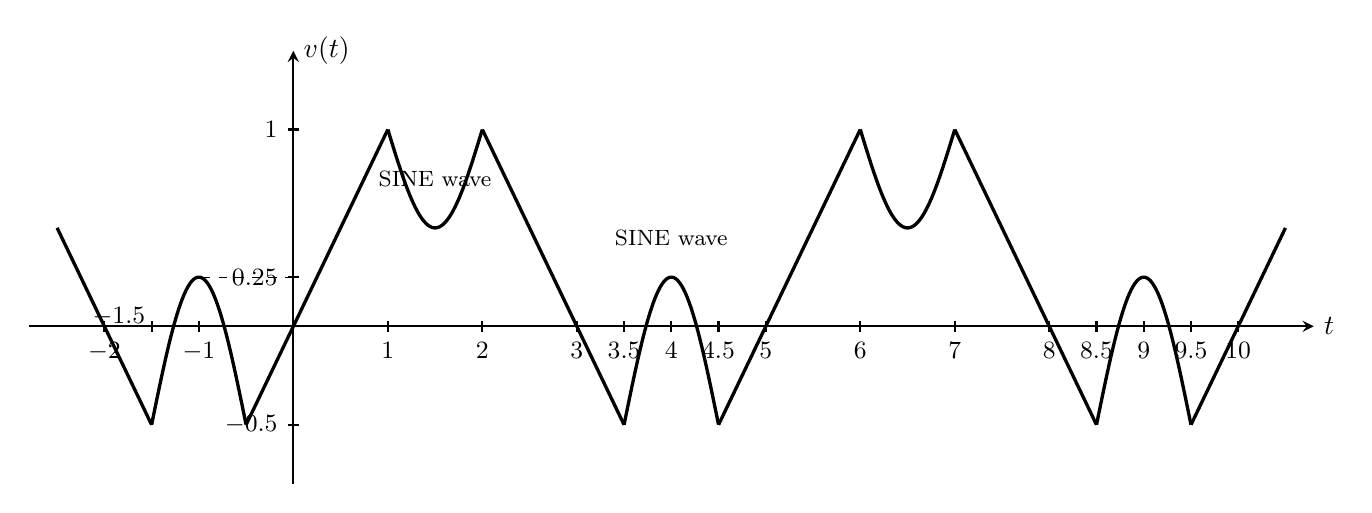
\begin{tikzpicture}[x=1.2cm, y=2.5cm, thick]

    % ---------------------------------------------------
    % Axes
    % ---------------------------------------------------
    \draw[->, >=stealth] (-2.8, 0) -- (10.8, 0) node[right] {$t$};
    \draw[->, >=stealth] (0, -0.8) -- (0, 1.4) node[right] {$v(t)$};

    % ---------------------------------------------------
    % Grid / Ticks for X-axis
    % ---------------------------------------------------
    \foreach \x in {-2, -1, 1, 2, 3, 3.5, 4, 4.5, 5, 6, 7, 8, 8.5, 9, 9.5, 10} {
        \draw (\x, 2pt) -- (\x, -2pt) node[below] {\small $\x$};
    }
    
    % Manual tick for -1.5 to match the image precisely
    \draw (-1.5, 2pt) -- (-1.5, -2pt) node[above left=-2pt] {\small $-1.5$};

    % ---------------------------------------------------
    % Grid / Ticks for Y-axis
    % ---------------------------------------------------
    \draw (2pt, 1) -- (-2pt, 1) node[left] {\small $1$};
    \draw (2pt, -0.5) -- (-2pt, -0.5) node[left] {\small $-0.5$};
    \draw (2pt, 0.25) -- (-2pt, 0.25) node[left] {\small $0.25$};

    % Dashed line pointing from the 0.25 tick to the left peak
    \draw[dashed, thin] (0, 0.25) -- (-1, 0.25);

    % ---------------------------------------------------
    % The Waveform
    % ---------------------------------------------------
    \begin{scope}[black, very thick]
        
        % Segment 1: t < 0
        \draw (-2.5, 0.5) -- (-2, 0);
        \draw (-2, 0) -- (-1.5, -0.5);
        % Lower sine hump (amplitude 0.75, base -0.5)
        \draw plot[domain=-1.5:-0.5, samples=50] (\x, {-0.5 + 0.75*sin((\x+1.5)*180)});
        \draw (-0.5, -0.5) -- (0, 0);

        % Segment 2: 0 < t < 5 (One full period)
        \draw (0, 0) -- (1, 1);
        % Upper sine dip (starts at 1, dips to 0.5)
        \draw plot[domain=1:2, samples=50] (\x, {1 - 0.5*sin((\x-1)*180)});
        \draw (2, 1) -- (3, 0);
        \draw (3, 0) -- (3.5, -0.5);
        % Lower sine hump
        \draw plot[domain=3.5:4.5, samples=50] (\x, {-0.5 + 0.75*sin((\x-3.5)*180)});
        \draw (4.5, -0.5) -- (5, 0);

        % Segment 3: 5 < t < 10 (Next full period)
        \draw (5, 0) -- (6, 1);
        \draw plot[domain=6:7, samples=50] (\x, {1 - 0.5*sin((\x-6)*180)});
        \draw (7, 1) -- (8, 0);
        \draw (8, 0) -- (8.5, -0.5);
        \draw plot[domain=8.5:9.5, samples=50] (\x, {-0.5 + 0.75*sin((\x-8.5)*180)});
        \draw (9.5, -0.5) -- (10, 0);
        
        % Segment 4: t > 10
        \draw (10, 0) -- (10.5, 0.5);
        
    \end{scope}

    % ---------------------------------------------------
    % Annotations
    % ---------------------------------------------------
    % Text "SINE wave" placed precisely where they appear
    \node[font=\footnotesize] at (1.5, 0.75) {SINE wave};
    \node[font=\footnotesize] at (4, 0.45) {SINE wave};
    
\end{tikzpicture}
\end{center}
\mk{15} \yr{EEE 163 | L-1/T-1 | 2006--07}

\item Determine the form factor and peak factor for the following voltage waveshape. The signal is periodic.
\begin{center}
   
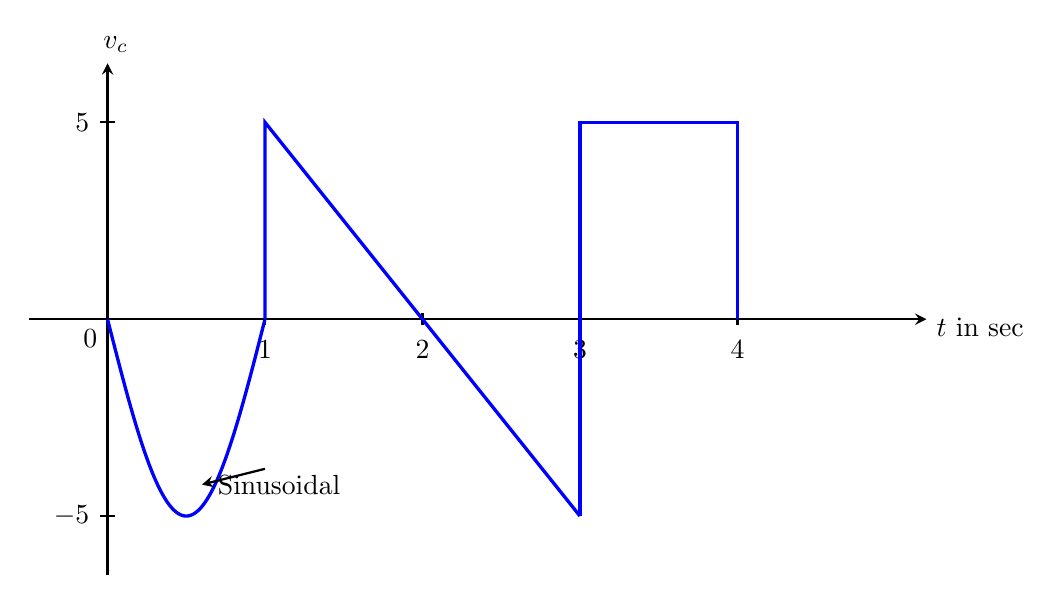
\begin{tikzpicture}[thick, xscale=2, yscale=0.5, >=stealth]

    % --- Axes ---
    % X-axis: time 't' in seconds
    \draw[->, thick] (-0.5, 0) -- (5.2, 0) node[right, yshift=-3pt] {$t \text{ in sec}$};
    % Y-axis: voltage 'v_c'
    \draw[->, thick] (0, -6.5) -- (0, 6.5) node[above, xshift=3pt] {$v_c$};

    % --- Axis Labels & Ticks ---
    % Origin
    \node[below left] at (0,0) {$0$};
    
    % Y-axis ticks
    \draw (0.05, 5) -- (-0.05, 5) node[left] {$5$};
    \draw (0.05, -5) -- (-0.05, -5) node[left] {$-5$};

    % X-axis ticks (1, 2, 3, 4)
    \foreach \x in {1, 2, 3, 4} {
        \draw (\x, 0.15) -- (\x, -0.15) node[below=2pt] {$\x$};
    }

    % --- Waveform Draw ---
    % 1. Sinusoidal half-cycle from t=0 to t=1 (pointing downwards)
    \draw[very thick, blue, domain=0:1, samples=100] plot (\x, {-5*sin(\x*180)});
    
    % Text pointer for 'Sinusoidal'
    \draw[->, bitext/.style={font=\footnotesize}] (1.0, -3.8) -- (0.6, -4.2) node[right, xshift=2pt] {Sinusoidal};

    % 2. Vertical jump at t=1, then linear decrease from (1,5) through (2,0) to (3,-5)
    \draw[very thick, blue] (1,0) -- (1,5) -- (3,-5);

    % 3. Vertical jump at t=3, then flat rectangular pulse at 5V until t=4, then drops to 0
    \draw[very thick, blue] (3,-5) -- (3,5) -- (4,5) -- (4,0);


\end{tikzpicture}
  
\end{center}
\mk{25} \yr{EEE 163 | L-1/T-1 | 2005--06}

\item The voltage waveshape $v_c$ shown below and 5(b) is applied across a capacitor of value $C = 1\,\mu\text{F}$. Draw the waveshape of the current $i_c$ passing through this capacitor.
\begin{center}
  
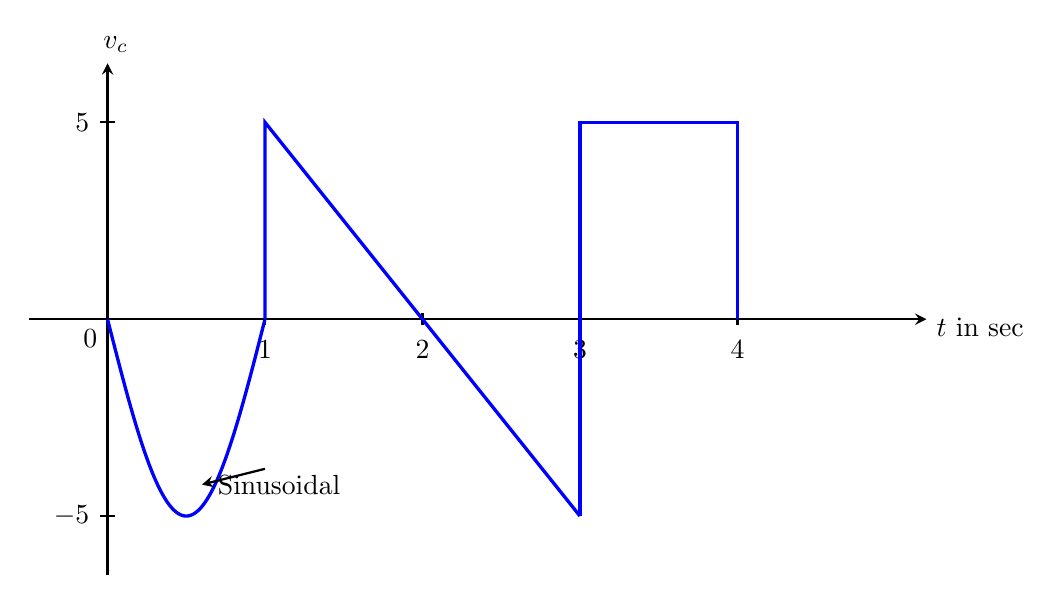
\begin{tikzpicture}[thick, xscale=2, yscale=0.5, >=stealth]

    % --- Axes ---
    % X-axis: time 't' in seconds
    \draw[->, thick] (-0.5, 0) -- (5.2, 0) node[right, yshift=-3pt] {$t \text{ in sec}$};
    % Y-axis: voltage 'v_c'
    \draw[->, thick] (0, -6.5) -- (0, 6.5) node[above, xshift=3pt] {$v_c$};

    % --- Axis Labels & Ticks ---
    % Origin
    \node[below left] at (0,0) {$0$};
    
    % Y-axis ticks
    \draw (0.05, 5) -- (-0.05, 5) node[left] {$5$};
    \draw (0.05, -5) -- (-0.05, -5) node[left] {$-5$};

    % X-axis ticks (1, 2, 3, 4)
    \foreach \x in {1, 2, 3, 4} {
        \draw (\x, 0.15) -- (\x, -0.15) node[below=2pt] {$\x$};
    }

    % --- Waveform Draw ---
    % 1. Sinusoidal half-cycle from t=0 to t=1 (pointing downwards)
    \draw[very thick, blue, domain=0:1, samples=100] plot (\x, {-5*sin(\x*180)});
    
    % Text pointer for 'Sinusoidal'
    \draw[->, bitext/.style={font=\footnotesize}] (1.0, -3.8) -- (0.6, -4.2) node[right, xshift=2pt] {Sinusoidal};

    % 2. Vertical jump at t=1, then linear decrease from (1,5) through (2,0) to (3,-5)
    \draw[very thick, blue] (1,0) -- (1,5) -- (3,-5);

    % 3. Vertical jump at t=3, then flat rectangular pulse at 5V until t=4, then drops to 0
    \draw[very thick, blue] (3,-5) -- (3,5) -- (4,5) -- (4,0);


\end{tikzpicture}

\end{center}
\mk{10} \yr{EEE 163 | L-1/T-1 | 2005--06}

\end{enumerate}

%%──────────────────────────────────────────────────────────────────────
\subtopic{cB}{Sinusoidal Signals \& Phasors}
\label{sub:s2-sinusoidal}

\begin{enumerate}\item Using the phasor approach, find the voltage $v(t)$ in a circuit described by the following equation:
\[2\frac{dv}{dt} + 5v + 10\int v\,dt = 20\cos(5t - 30^\circ)\]
\mk{5} \yr{EEE 163 | L-1/T-1 | 2015--16}

\item A voltage $v = 100\cos(314.16t)$ is applied to a circuit and it is determined that the current $i$ is $5\sin(314.16t + 60^\circ)$. Determine the nature of the circuit elements. Also, find the values of the circuit parameters.
\mk{10} \yr{EEE 163 | L-1/T-1 | 2013--14}

\item A voltage $v = 200\cos(157t + 30^\circ)$\,V is applied to a particular circuit element, and it is found that $i = 5\sin(157t - 150^\circ)$\,A. Sketch $v$ and $i$ waves. Find the nature and magnitude of the circuit parameter(s).
\mk{10} \yr{EEE 163 | L-1/T-1 | 2012--13}

\item What is the phase relationship between the sinusoidal waveforms of each of the following sets?
\begin{enumerate}
  \item $i = -2\cos(\omega t - 60^\circ)$, $v = 3\sin(\omega t - 150^\circ)$
  \item $i = -2\sin(\omega t + 10^\circ)$, $v = -4\cos(\omega t + 90^\circ)$
\end{enumerate}
\mk{3+3} \yr{EEE 163 | L-1/T-1 | 2006--07}

\item Draw the complete vector (phasor) diagram of the circuit shown below.
\begin{center}
  \begin{tikzpicture}[x=1.5cm, y=1.5cm, thick]

    % ---------------------------------------------------
    % Bottom wire and Ground
    % ---------------------------------------------------
    \draw (0,0) node[ground] {} -- (8,0);
    
    % ---------------------------------------------------
    % AC Source (Left Branch)
    % ---------------------------------------------------
    \draw (0,0) to[sV] (0,3);
    \node at (-0.5, 2.3) {$+$};
    \node at (-1.1, 1.5) {$V_{in}$};
    \node at (-0.5, 0.7) {$-$};
    
    % ---------------------------------------------------
    % Top Branch (R and L)
    % ---------------------------------------------------
    % Resistor (V5)
    \draw (0,3) to[R] (2.5,3);
    \node at (0.3, 3.4) {$+$};
    \node at (1.25, 3.4) {$V_5$};
    \node at (2.2, 3.4) {$-$};
    
    % Inductor (V4)
    \draw (2.5,3) to[L] (5,3);
    \node at (2.8, 3.4) {$-$};
    \node at (3.75, 3.5) {$V_4$};
    \node at (4.7, 3.4) {$+$};
    
    % Top wire continuing to the right
    \draw (5,3) -- (8,3);
    
    % Current I
    \draw[->, >=stealth] (0.7, 2.4) -- (1.8, 2.4) node[midway, below] {$I$};
    
    % Current I4
    \draw[->, >=stealth] (6, 3.4) -- (7, 3.4) node[midway, above] {$I_4$};
    
    % ---------------------------------------------------
    % Middle Vertical Branch
    % ---------------------------------------------------
    % Top part: Resistor (V2)
    \draw (5,1.5) to[R] (5,3);
    \node at (4.6, 2.7) {$+$};
    \node at (4.3, 2.25) {$V_2$};
    \node at (4.6, 1.8) {$-$};
    
    % Current I3 (pointing UP)
    \draw[<-, >=stealth] (5.5, 2.8) -- (5.5, 1.7) node[midway, right] {$I_3$};
    
    % Bottom part: Parallel LC combination (V1)
    \draw (5,1.5) -- (4,1.5) to[L] (4,0) -- (5,0); % Left Inductor
    \draw (5,1.5) -- (6,1.5) to[C] (6,0) -- (5,0); % Right Capacitor
    
    % Currents I1 and I2
    \draw[->, >=stealth] (3.4, 1.1) -- (3.4, 0.4) node[midway, left] {$I_1$};
    \draw[->, >=stealth] (6.6, 1.1) -- (6.6, 0.4) node[midway, right] {$I_2$};
    
    % Voltage V1 Label (Inside the parallel block)
    \node at (5, 1.2) {$+$};
    \node at (5, 0.75) {$V_1$};
    \node at (5, 0.3) {$-$};
    
    % ---------------------------------------------------
    % Rightmost Branch (Capacitor V3)
    % ---------------------------------------------------
    \draw (8,3) to[C] (8,0);
    \node at (8.6, 2.5) {$-$};
    \node at (8.6, 1.5) {$V_3$};
    \node at (8.6, 0.5) {$+$};

    
\end{tikzpicture}
\end{center}
\mk{14} \yr{EEE 163 | L-1/T-1 | 2006--07}

\end{enumerate}

%%──────────────────────────────────────────────────────────────────────
\subtopic{cB}{RL Circuits}
\label{sub:s2-rl}

\begin{enumerate}\item If a current, $i(t) = I_m \sin(\omega t)$, is flowing through an RL series circuit, derive the expression of instantaneous voltage and instantaneous power of this circuit. Also, illustrate the waveshapes of the instantaneous voltage and the instantaneous power of the series circuit.
\mk{12} \yr{EEE 163 | L-1/T-1 | 2022--23}

\item An industrial coil is modelled as a series combination of an inductance $L$ and resistance $R$, as shown below. Given $|V_s| = 145$\,V, $|V_1| = 50$\,V, $|V_o| = 110$\,V. Determine the values of $L$ and $R$.
\begin{center}
  \begin{tikzpicture}[thick, american, scale=1.4]
    
    % Main circuit loop baseline
    \draw (0,0) -- (4,0);
    
    % Left branch: Independent AC voltage source Vs
    \draw (0,0) to[V, l=$V_s$] (0,3);
    
    % Top horizontal branch: 80 ohm resistor with voltage drop V1
    \draw (0,3) to[R, l=$80\,\Omega$, v=$V_1$] (4,3);
    
    % --- COIL SUB-CIRCUIT (Dotted Box) ---
    % Vertical connections inside the coil
    \draw (4,3) -- (4,2.2)
                to[R, l=$R$] (4,1.2)
                to[L, l=$L$] (4,0);
                
    % Drawing the dashed boundary box around the coil components
    \draw[dashed, line width=0.6pt] (3.2,-0.2) rectangle (4.6,3.2);
    
    % Text Label for the Coil outside the dashed box
    \node[anchor=west] at (4.6,3.1) {Coil};
    
    % Output voltage Vo labels along the side of the dashed box
    \node at (4.9,2.5) {$+$};
    \node at (5.0,1.5) {$V_o$};
    \node at (4.9,0) {$-$};

\end{tikzpicture}

\end{center}
\mk{20} \yr{EEE 163 | L-1/T-1 | 2020--21}

\item Assume that a current wave $i(t) = I_m\sin\omega t$ flows through a R--L branch. Derive the expressions for voltage wave, impedance, instantaneous power and average power. Write down the expressions for instantaneous real power, instantaneous reactive power, real power and reactive power. Also draw the waveshape of instantaneous power.
\mk{25} \yr{EEE 163 | L-1/T-1 | 2012--13}

\item Assume that the current $i(t) = I_m\sin\omega t$ flows through a series RL branch. Derive the expressions for applied voltage, impedance, instantaneous power, real power and reactive power. Also draw the wave shape for power.
\mk{20} \yr{EEE 163 | L-1/T-1 | 2010--11}

\item A voltage $v(t) = 141.4\cos(100t)$\,V is applied to a series circuit and the resulting current is found to be $i(t) = 0.707\cos(100t - 53.13^\circ)$\,A. One element of this series combination is an inductance of 1800\,mH. Determine the magnitude of the other series elements present.
\mk{15} \yr{EEE 163 | L-1/T-1 | 2010--11}

\end{enumerate}

%%──────────────────────────────────────────────────────────────────────
\subtopic{cB}{RC Circuits}
\label{sub:s2-rc}

\begin{enumerate}
  
\item Assume that a current $i = I_m\sin\omega t$ flows through a series RC circuit. Derive the expressions for applied voltage ($V$), total impedance ($Z$), instantaneous power ($p$), real power ($P$), reactive power ($Q$) and apparent power ($S$). Also draw the wave shape for power.
\mk{20} \yr{EEE 163 | L-1/T-1 | 2024--25, 2014--15}

\item Find out the power factor of the circuit shown below. To what value must the 10\,$\mu$F capacitor be changed to result in an overall power factor of 0.95 lagging?
\begin{center}
  \begin{circuitikz}[scale=1.2, transform shape, thick]

    % Left-most side: Double-headed arrow indicating input voltage source properties
    \draw[<->, >=stealth] (0,0) -- (0,3);
    \node at (0.2, 1.5) [right, align=left] {100V\\50\,Hz};

    % Top horizontal connecting wire
    \draw (0,3) -- (5,3);
    
    % Bottom horizontal connecting wire
    \draw (0,0) -- (5,0);

    % Middle vertical branch: 18 Ohm resistor in series with a 0.5 H inductor
    \draw (2.5,3) to[R, l=$18\,\Omega$] (2.5,1.5)
                  to[L, l=$0.5\text{ H}$] (2.5,0);

    % Far right vertical branch: 10 uF capacitor
    \draw (5,3) to[C, l=$10\,\mu\mathrm{F}$] (5,0);


\end{circuitikz}

\end{center}
\mk{15} \yr{EEE 163 | L-1/T-1 | 2014--15}

\item Assume that the current $i(t) = I_m\sin\omega t$ flows through a series R--C branch. Derive the expressions for applied voltage, impedance, instantaneous power, real power and reactive power. Also draw the waveshape for power.
\mk{20} \yr{EEE 163 | L-1/T-1 | 2011--12}

\item For the series RC circuit, assume that the current $I = I_m \sin\omega t$ flows through the circuit. Show that the voltage across the branch is $v = I_m|Z|\sin(\omega t + \theta) = V_m \sin(\omega t + \theta)$ where $|Z| = \sqrt{R^2 + (-\frac{1}{\omega C})^2}$ and $\theta = -\tan^{-1}\frac{1}{\omega RC}$. Draw the waveshapes for different components of instantaneous power and also determine the average power absorbed by the RC branch.
\mk{10+6+4} \yr{EEE 163 | L-1/T-1 | 2006--07}

\end{enumerate}

%%──────────────────────────────────────────────────────────────────────
\subtopic{cB}{RLC Circuits}
\label{sub:s2-rlc}

\begin{enumerate}\item If a current, $i(t) = I_m \sin(\omega t)$, is flowing through an RLC series circuit, derive the expression of instantaneous voltage and instantaneous power of this circuit. Also, illustrate the waveshapes of the instantaneous voltage and the instantaneous power of the series circuit.
\mk{10} \yr{EEE 163 | L-1/T-1 | 2023--24}

\item For the series RLC circuit shown below, find out the value of capacitor $C$ for which the input current $I$ leads the voltage $V_s$ by 30 degrees. Draw the phasor diagram for the circuit considering the obtained value of $C$.
\begin{center}
  \begin{tikzpicture}[thick, scale=1.5]

    % Bottom wire line connection
    \draw (0,0) -- (4,0);

    % Left open voltage terminal indicator (Vs)
    \draw (0,2) to[open, v=$V_s$] (0,0);
    \draw (3,1) node[left]{$120\,\text{V}_{\text{p-p}}$};
        \draw (3,0.6) node[left]{$50 Hz Sinusoid$};

    % Top horizontal line containing the series Resistor and Inductor
    % Including current arrow 'I' pointing to the right
    \draw (0,2) to[short, i=$I$] (0.8,2)
                to[R, l={$R=100\,\Omega$}] (2.2,2)
                to[L, l={$L=22\text{ mH}$}] (4,2);

    % Right vertical branch containing the Capacitor C
    \draw (4,2) to[C, l=$C$] (4,0);

\end{tikzpicture}

\end{center}
\mk{15} \yr{EEE 163 | L-1/T-1 | 2021--22}

\item For the circuit shown below, find out the expression for the frequency at which the output voltage $V_0$ equals the input voltage $V_i$. By choosing $R = 100\,\Omega$, $L = 22$\,mH and $C = 47\,\mu$F, sketch the magnitude of the output voltage versus frequency.
\begin{center}
  \begin{tikzpicture}[thick, scale=1.5]

    % Bottom wire line connection
    \draw (0,0) -- (4,0);

    % Left open input voltage terminal indicator (Vi)
    \draw (0,2) to[open, v=$V_i$] (0,0);

    % Top horizontal line through the series resistor R
    \draw (0,2) to[R, l=$R$] (2.2,2);

    % First parallel vertical branch: Inductor L
    \draw (2.2,2) to[L, l_=$L$] (2.2,0);

    % Connect top and bottom lines to the second parallel branch
    \draw (2.2,2) -- (3.2,2);
    \draw (2.2,0) -- (3.2,0);

    % Second parallel vertical branch: Capacitor C
    \draw (3.2,2) to[C, l=$C$] (3.2,0);

    % Extensions to the open output voltage terminals (Vo)
    \draw (3.2,2) -- (4,2) node[circle, draw, fill=white, inner sep=1pt] {};
    \draw (3.2,0) -- (4,0) node[circle, draw, fill=white, inner sep=1pt] {};
    
    % Output voltage label Vo with +/- polarity indicators
    \draw (4,2) to[open, v_=$V_o$] (4,0);

    % Standard T-junction connection dots
    \fill (2.2,2) circle (1.5pt);
    \fill (2.2,0) circle (1.5pt);
    \fill (3.2,2) circle (1.5pt);
    \fill (3.2,0) circle (1.5pt);

\end{tikzpicture}

\end{center}
\mk{20} \yr{EEE 163 | L-1/T-1 | 2021--22}

\item In the circuit shown below, calculate the value of inductance $L$ across the R--C series combination so that the net impedance is resistive at a frequency of 5\,MHz.
\begin{center}
  \begin{tikzpicture}[thick, american, scale=1.4]
    
    % Input terminals on the left (small open circles)
    \draw (0,2) circle (1.5pt);
    \draw (0,0) circle (1.5pt);
    
    % Top and bottom horizontal rails connecting the branches
    \draw (0,2) -- (2,2);
    \draw (0,0) -- (2,0);
    
    % First vertical branch: Inductor L
    \draw (1,2) to[L, l_=$L$] (1,0);
    
    % Second vertical branch: Resistor in series with a Capacitor
    \draw (2,2) to[R, l=$200\,\Omega$] (2,1)
                to[C, l=$50\text{ nF}$] (2,0);

    % Connection dots at the top and bottom junctions of the first branch
    \fill (1,2) circle (1.5pt);
    \fill (1,0) circle (1.5pt);

\end{tikzpicture}

\end{center}
\mk{15} \yr{EEE 163 | L-1/T-1 | 2020--21}

\item Assume that a current $i(t) = I_m\sin(\omega t)$ flows through a series RLC circuit. Derive the expressions for applied voltage ($V$), total impedance ($Z$), instantaneous power ($p$), real power ($P$), reactive power ($Q$) and apparent power ($S$). Also draw the wave shape for power.
\mk{15} \yr{EEE 163 | L-1/T-1 | 2017--18}

\item A voltage $v = 100\sin(314t + 45^\circ)$ is applied to a series circuit and the resulting current is found to be $i = 20\sin(314t - 15^\circ)$. Find the elements comprising the circuit. Draw the waves of $v$, $i$ and the voltage across the reactive element ($v_x$). Also, draw the phasor diagram for $V$, $I$, $V_x$ and $V_R$.
\mk{15} \yr{EEE 163 | L-1/T-1 | 2008--09}

\item Assume that the current $i = I_m\sin\omega t$ flows through a given RLC series circuit. Show that the voltage across this branch is $v = I_m|Z|\sin(\omega t+\theta) = V_m\sin(\omega t+\theta)$ where $|Z| = \sqrt{R^2+(\omega L - \frac{1}{\omega C})^2}$ and $\theta = \tan^{-1}\frac{\omega L - \frac{1}{\omega C}}{R}$. If $L = 0.1$\,H, $C = 1\,\mu\text{F}$ and $R = 100\,\Omega$, what will be the frequency $f$ so that the impedance $|Z|$ is minimum?
\mk{12+8} \yr{EEE 163 | L-1/T-1 | 2007--08}

\item For the RLC parallel circuit shown below, $v = V_m \cos\omega t$. Derive the expression for the instantaneous current $i$ passing from the source.
\begin{center}
  \begin{tikzpicture}[thick,>=stealth]

    % --- Leftmost Branch (AC Voltage Source) ---
    % Sinusoidal voltage source labeled 'v'
    \draw (0,0) to[vsourcesin, l=$v$] (0,3);

    % --- Top Wire with Current 'i' ---
    % Current flowing from left to right before reaching the branches
    \draw (0,3) to[short, i=$i$] (2.5,3);

    % --- Parallel Resistor Branch ---
    \draw (2.5,3) to[R, l=$R$] (2.5,0);

    % --- Parallel Inductor Branch ---
    \draw (2.5,3) -- (4.5,3) to[L, l=$L$] (4.5,0);

    % --- Parallel Capacitor Branch ---
    \draw (4.5,3) -- (6.5,3) to[C, l=$C$] (6.5,0);

    % --- Bottom Common Wire ---
    \draw (0,0) -- (6.5,0);

    % --- Junction Dots ---
    \fill (2.5,3) circle (2pt);
    \fill (2.5,0) circle (2pt);
    \fill (4.5,3) circle (2pt);
    \fill (4.5,0) circle (2pt);

\end{tikzpicture}
\end{center}
\mk{17} \yr{EEE 163 | L-1/T-1 | 2005--06}

\end{enumerate}

%%──────────────────────────────────────────────────────────────────────
\subtopic{cB}{Power in AC Circuits}
\label{sub:s2-power}

\begin{enumerate}


\item Find $I_1$ and voltage across $2 \text{ k}\Omega$ resistor for the circuit shown below (a). 
What is the real, reactive and apparent power provided by the independent current 
source? Also, find the real power consumed by $1 \text{ k}\Omega$ resistor.  
  
\begin{center}
  \begin{tikzpicture}[thick, scale=1.5, x=1.4cm ]

    % --- BASE GROUND WIRE RAIL ---
    \draw (0,0) -- (4.2,0);

    % --- LEFTMOST BRANCH ---
    % 5 mA Phasor Current Source (pointing up)
    \draw (0,0) to[I, l=$5\text{ mA }\angle\ 0^\circ$] (0,1.8) -- (1.2,1.8);

    % --- FIRST VERTICAL INTERMEDIATE BRANCH ---
    % 2 kohm Resistor with voltage drop Vx across it
    \draw (1.2,1.8) to[R, l=$2\text{ k}\Omega$, v=$V_x$] (1.2,0);

    % --- MAIN MIDDLE HORIZONTAL WIRE SEGMENTS ---
    % Dependent Sinusoidal Voltage Source (2*Vx) with inverted polarity labels (- on left, + on right)
    \draw (2.8,1.8) to[cvsourcesin, v=$2V_x$,] (1.2,1.8);

    % --- OVERHEAD PARALLEL BYPASS BRIDGE ---
    % Upper branch containing the 1 kohm resistor with current label I1 pointing right
    \draw (1.2,1.8) -- (1.2,2.6)
                    to[R, l=$1\text{ k}\Omega$, i^=$I_1$] (2.8,2.6)
                    -- (2.8,1.8);

    % --- SECOND VERTICAL INTERMEDIATE BRANCH ---
    % Dependent Current Source (3*I1) pointing downwards
    \draw (2.8,1.8) to[cisource, l=$3I_1$] (2.8,0);

    % --- RIGHTMOST VERTICAL BRANCH ---
    % 1 kohm termination resistor
    \draw (2.8,1.8) -- (4.2,1.8)
                    to[R, l=$1\text{ k}\Omega$] (4.2,0);

    % --- JUNCTION NODES ---
    \fill (1.2,1.8) circle (1.5pt);
    \fill (2.8,1.8) circle (1.5pt);
    \fill (1.2,0)   circle (1.5pt);
    \fill (2.8,0)   circle (1.5pt);

\end{tikzpicture}

\end{center}

\mk{17} \yr{EEE 163 | L-1/T-1 | 2024--25}



\item Find $I$ for the circuit shown below. What is the real, reactive and apparent power provided by the voltage source? Also, find the real power consumed by 3\,$\Omega$. [The circuit contains: $R_1 = 2\,\Omega$, $R_2 = 3\,\Omega$, $R_3 = 10\,\Omega$, $X_L = 6\,\Omega$, $X_{C1} = 9\,\Omega$, $X_{C2} = 2\,\Omega$; Source: $E = 50\,\text{V}\angle 0^\circ$.]
\begin{center}
  \begin{circuitikz}[thick , american, scale=1.2, transform shape]

    % Coordinates for the bridge nodes
    \coordinate (A) at (2.5,4.5);
    \coordinate (B) at (2.5,0);
    \coordinate (C) at (8.5,4.5);
    \coordinate (H) at (8.5,0);
    
    % Jump coordinates at the center intersection
    \coordinate (Before) at ($(A)!0.46!(H)$);
    \coordinate (After) at ($(A)!0.54!(H)$);

    % Left side: AC Sinusoidal Voltage Source and Ground
    \draw (0,0) to[vsourcesin, l={$\mathbf{E} = 50\text{ V}\angle 0^\circ$}] (0,4.5);
    \draw (0,0) node[ground]{};
    
    % Explicit Polarity signs (+ and -) for the AC source
    \node[above right] at (0, 3.6) {$+$};
    \node[below right] at (0, 0.9) {$-$};

    % Top and Bottom main wires with Current 'I' arrow
    \draw (0,4.5) to[short, i=$\mathbf{I}$] (A) -- (C);
    \draw (0,0) -- (B) -- (H);

    % Diagonal Branch 1: From Node 'b' to 'c' (Passes underneath)
    \draw (B) to[L, l=$6\ \Omega$, a_=$X_L$] ($(B)!0.25!(C)$)
              to[C, l=$9\ \Omega$, a_=$X_{C_1}$] ($(B)!0.45!(C)$)
              -- ($(B)!0.68!(C)$)
              to[R, l=$3\ \Omega$, a_=$R_2$] (C);

    % Diagonal Branch 2: From Node 'a' to 'h' (Jumps over the center)
    \draw (A) to[R, l=$2\ \Omega$, a_=$R_1$] ($(A)!0.32!(H)$) 
              -- (Before) 
              to[out=45, in=135] (After) % The bridge jump effect
              -- ($(A)!0.68!(H)$) 
              to[C, l=$2\ \Omega$, a_=$X_{C_2}$] (H);

    % Rightmost vertical branch with R3
\draw (C) to[R, l=$R_3$, a_=$10\ \Omega$] (H);
    % Labeling the specific nodes (a, b, c, h)
    \node[below left] at (A) {a};
    \node[below left] at (B) {b};
    \node[above right] at (C) {c};
    \node[below right] at (H) {h};

\end{circuitikz}
\end{center}
\mk{18} \yr{EEE 163 | L-1/T-1 | 2023--24}

\item The load impedance $Z_L$ for the circuit shown below is adjusted until maximum average power is delivered to $Z_L$.
\begin{enumerate}
  \item Find the maximum average power delivered to $Z_L$.
  \item Determine the power factor of this load.
  \item What percentage of the total power developed in the circuit is delivered to $Z_L$?
\end{enumerate}
\begin{center}
  
\begin{circuitikz}[thick,american, scale=1.2, transform shape]

    % Left Independent AC Voltage Source
    % Drawn from bottom to top so the label stays on the left
    \draw (0,3) to[V, l=$100\angle0^\circ\text{ V (rms)}$] (0,0);

    % Top horizontal branch (Resistor and Inductor with current I_phi)
    % i_ puts the current arrow and label below the wire
    \draw (0,3) to[R, l=$25\ \Omega$, i_=$\mathbf{I}_\phi$] (2.5,3)
                to[L, l=$j10\ \Omega$, -*] (5,3);

    % Dependent Voltage Source in the middle
    % Drawn from top to bottom so '+' is at the top node
    \draw (5,3) to[cV, l=$5\mathbf{I}_\phi$] (5,0);

    % Top wire continues to a 1 Ohm resistor
    \draw (5,3) to[R, l=$1\ \Omega$, -*] (8,3);

    % Right vertical branch with j3 Ohm Inductor
    \draw (8,3) to[L, l=$j3\ \Omega$] (8,0);

    % Connections to the open terminals before the Load
    \draw (8,3) -- (9.5,3) node[circ]{};
    \draw (8,0) -- (9.5,0) node[circ]{};

    % Load Impedance Z_L (Variable)
    \draw (9.5,3) -- (11,3) to[generic, l=$Z_L$] (11,0) -- (9.5,0);
    
    % Diagonal arrow across Z_L to indicate it is a variable load
    \draw[-latex, thick] (10.4, 0.6) -- (11.6, 2.4);

    % Bottom return wire connecting all vertical branches
    \draw (0,0) -- (5,0) node[circ]{} 
          -- (8,0) node[circ]{} 
          -- (9.5,0);

   

\end{circuitikz}
\end{center}
\mk{20} \yr{EEE 163 | L-1/T-1 | 2023--24}

\item Calculate $Z_T$ for the circuit of the given Figure. Also, compute the real and reactive power supplied by the $100\angle 60^\circ\,\text{V}$ voltage source, if $Z_T$ is connected to this source as load.
\begin{center}
  
\begin{tikzpicture}[thick, x=1.5cm, y=1.5cm, >=stealth]
    
    % Input Terminals
    \draw (0, 3) node[ocirc] (T1) {};
    \draw (0, 0) node[ocirc] (T2) {};
    
    % Z_T Label and Arrow
    \draw[->, thick] (-0.3, 1.5) -- (0.8, 1.5) node[midway, above] {$\mathbf{Z_T}$};

    % Top Series Input Branch (Resistor & Capacitor)
    \draw (T1) to[R, l=$8\,\Omega$] (1.5, 3) 
               to[C, l={$-j12\,\Omega$}] (3, 3);
               
    % Bottom Input Branch (Straight Wire)
    \draw (T2) -- (3, 0);

    % --- Bridge Circuit Section ---
    
    % Left Vertical Arm (Resistor & Inductor)
    \draw (3, 3) to[R, l_=$20\,\Omega$] (3, 1.5) 
                 to[L, l_=$j15\,\Omega$] (3, 0);

    % Top Horizontal Arm (Capacitor)
    \draw (3, 3) to[C, l={$-j16\,\Omega$}] (6, 3);

    % Bottom Horizontal Arm (Capacitor)
    \draw (3, 0) to[C, l={$-j16\,\Omega$}] (6, 0);

    % Right Vertical Arm (Two Resistors)
    \draw (6, 3) to[R, l=$10\,\Omega$] (6, 1.5) 
                 to[R, l=$10\,\Omega$] (6, 0);

    % Center Horizontal Cross-Arm (Resistor)
    \draw (3, 1.5) to[R, l=$10\,\Omega$] (6, 1.5);
    

\end{tikzpicture}
\end{center}

\mk{18} \yr{EEE 163 | L-1/T-1 | 2022--23}

\item In the circuit of the given figure, find the value of load impedance $Z_L$ that will absorb the maximum power and the value of the maximum power. Also, determine the power factor of this load.
\begin{center}
  
\begin{tikzpicture}[x=1.5cm, y=1.5cm, >=stealth, thick]

    % Bottom reference rail
    \draw (0, 0) -- (6, 0);

    % Left branch: AC Voltage Source
    % Drawing from bottom to top places the positive terminal at the top
    \draw (0, 2) to[V, l=$165\angle 0^\circ\,\mathrm{V}$] (0, 0);

    % Top bypass branch: Inductor
    \draw (0, 2) -- (0, 3.5) 
                 to[L, l=$j2\,\Omega$] (6, 3.5) 
                 -- (6, 2);

    % Middle horizontal branch: Resistor and Capacitor
    \draw (0, 2) to[R, l=$4\,\Omega$] (3, 2) 
                 to[C, l={$-j3\,\Omega$}] (6, 2);

    % Center vertical branch: Generic Impedance Block Z_L
    % Using 'european resistor' naturally renders the empty rectangular impedance box
    \draw (3, 2) to[european resistor, l_=$Z_L$] (3, 0);

    % Right vertical branch: Resistor
    \draw (6, 2) to[R, l_=$5\,\Omega$] (6, 0);

\end{tikzpicture}

\end{center}
\mk{23} \yr{EEE 163 | L-1/T-1 | 2022--23}

\item What is meant by power factor improvement and why do we need it? Illustrate with necessary figures and explain how power factor can be improved for both inductive and capacitive loads.
\mk{15} \yr{EEE 163 | L-1/T-1 | 2021--22}

\item Find out the average power absorbed by the 40\,$\Omega$ resistor in the circuit shown below.
\begin{center}
  \begin{tikzpicture}[thick, scale=1.5]

    % Bottom ground reference wire
    \draw (0,0) -- (5,0);

    % Leftmost AC independent current source branch (pointing up)
    \draw (0,0) to[I, l=$6\angle 0^\circ\text{ A}(50 Hz)$] (0,2) -- (1.5,2);

    % First vertical branch: 35 mH Inductor
    \draw (1.5,2) to[L, l=$35\text{ mH}$] (1.5,0);

    % Middle horizontal bridge branch with 220 uF Capacitor
    % Includes the controlling current Io pointing to the right
    \draw (1.5,2) to[C, l=$220\,\mu\text{F}$, i>_=$I_o$] (3.8,2);

    % Upper overhead bridge: 22 mH Inductor
    \draw (1.5,2) -- (1.5,2.8)
                  to[L, l=$22\text{ mH}$] (3.8,2.8)
                  -- (3.8,2);

    % Vertical dependent current source branch (pointing up)
    \draw (3.8,0) to[cisource, l=$0.5I_o$] (3.8,2);

    % Rightmost vertical branch: 40 ohm Resistor
    \draw (3.8,2) -- (5,2)
                  to[R, l=$40\,\Omega$] (5,0);

    % T-junction connection dots for visual clarity
    \fill (1.5,2) circle (1.5pt);
    \fill (3.8,2) circle (1.5pt);
    \fill (1.5,0) circle (1.5pt);
    \fill (3.8,0) circle (1.5pt);

\end{tikzpicture}

\end{center}
\mk{20} \yr{EEE 163 | L-1/T-1 | 2021--22}

\item If the voltage $v(t)$ shown below is applied across an impedance of $1 + j2$, find out the complex power delivered to the impedance.
\begin{center}
  \begin{tikzpicture}[ y=0.25cm]
    % Grid / Horizontal Voltage Level Lines
    \draw[dashed, gray!60, line width=0.5pt] (-0.5, 10) -- (13, 10);
    \draw[dashed, gray!60, line width=0.5pt] (-0.5, -10) -- (13, -10);
    \draw[dashed, gray!60, line width=0.5pt] (-0.5, -15) -- (13, -15);

    % Axes
    \draw[->, >=stealth, line width=0.8pt] (-0.5, 0) -- (13.5, 0) node[right] {$\omega t$};
    \draw[->, >=stealth, line width=0.8pt] (0, -18) -- (0, 14) node[above] {$v(t) \text{ in volts}$};

    % Y-Axis Labels
    \node[left, font=\small] at (0, 10) {$10$};
    \node[left, font=\small] at (0, 0) {$0$};
    \node[left, font=\small] at (0, -10) {$-10$};
    \node[left, font=\small] at (0, -15) {$-15$};

    % Waveform Plot (Two full periods)
    \draw[ultra thick, blue!80!black, line cap=round, line join=round] 
        (0,0) 
        sin (1.5708, 10) 
        cos (3.1416, 0) -- 
        (3.9270, 0) -- 
        (3.9270, -10) -- 
        (4.7124, -15) -- 
        (4.7124, 0) -- 
        (6.2832, 0)
        % Second Cycle
        sin (7.8540, 10) 
        cos (9.4248, 0) -- 
        (10.2102, 0) -- 
        (10.2102, -10) -- 
        (10.9956, -15) -- 
        (10.9956, 0) -- 
        (12.5664, 0);

    % X-Axis Ticks & Labels (Cycle 1)
    \draw[line width=0.6pt] (3.1416, 0.3) -- (3.1416, -0.3);
    \node[below, font=\small, yshift=-2pt] at (3.1416, 0) {$\pi$};
    
    \draw[line width=0.6pt] (3.9270, 0.3) -- (3.9270, -0.3);
    \node[above, font=\small, xshift=-8pt, yshift=2pt] at (3.9270, 0) {$\dfrac{5\pi}{4}$};
    
    \draw[line width=0.6pt] (4.7124, 0.3) -- (4.7124, -0.3);
    \node[above right, font=\small, xshift=-2pt, yshift=2pt] at (4.7124, 0) {$\dfrac{3\pi}{2}$};
    
    \draw[line width=0.6pt] (6.2832, 0.3) -- (6.2832, -0.3);
    \node[below right, font=\small] at (6.2832, 0) {$2\pi$};

\end{tikzpicture}

\end{center}
\mk{18} \yr{EEE 163 | L-1/T-1 | 2021--22}

\item Two loads are connected in parallel with a 50\,Hz voltage source $v(t) = 120\angle 10^\circ$. Load~1 draws 2.5\,kW at 0.8\,pf lagging and Load~2 draws 1.5\,kW at 0.5\,pf leading. Determine the values of $R_1$, $R_2$, $L$ and $C$ in the circuit. Using the obtained values, calculate the current supplied by the source.
\begin{center}
  \begin{tikzpicture}[thick, scale=1.4, >=Stealth]

    % Bottom wire line connection
    \draw (0,0) -- (4.5,0);
    
    % Ground connection node
    \draw (2.2,0) node[ground] {};

    % Leftmost branch: AC Voltage Source
    \draw (0,0) to[V, invert, l=$v(t)$, a={$120\angle 0^\circ$}] (0,2.5);
    % Main top rail wire connection
    \draw (0,2.5) -- (4.5,2.5);

    % --- LOAD 1 BRANCH ---
    % Vertical branch: Resistor R1 and Inductor L in series
    \draw (2.2,2.5) to[R, l=$R_1$] (2.2,1.3)
                    to[L, l=$L$] (2.2,0);

    % Dashed bounding box for Load 1
    \draw[dashed, thin] (1.8,0.1) rectangle (2.6,2.4);
    
    % Annotation arrow and label for Load 1
    \draw[<-] (2.65,0.9) -- (3.1,0.7) node[right, font=\small] {Load 1};


    % --- LOAD 2 BRANCH ---
    % Vertical branch: Resistor R2 and Capacitor C in series
    \draw (4.5,2.5) to[R, l=$R_2$] (4.5,1.3)
                    to[C, l=$C$] (4.5,0);

    % Dashed bounding box for Load 2
    \draw[dashed, thin] (4.1,0.4) rectangle (4.9,2.4);
    
    % Annotation arrow and label for Load 2
    \draw[<-] (4.95,1.1) -- (5.4,0.9) node[right, font=\small] {Load 2};

\end{tikzpicture}

\end{center}
\mk{17} \yr{EEE 163 | L-1/T-1 | 2021--22}

\item For the circuit below, find $I_o$ and the input power factor.
\begin{center}
  \begin{tikzpicture}[thick, american, scale=1.4]
    
    % Bottom horizontal rail
    \draw (0,0) -- (4.2,0);
    
    % Top horizontal rail with current indicator Io
    \draw (0,2) -- (4.2,2);
    \draw[-{Stealth}, thick] (0.3,2.2) -- (0.7,2.2) node[midway, above] {$I_o$};
    
    % Leftmost branch: AC voltage source 220\angle 0^\circ V (RMS)
    \draw (0,2) to[V, l_=$220\angle 0^\circ\text{ V}(RMS)$] (0,0);
    
    % First load box (12 kW, 0.866 pf leading)
    \draw (2,2) -- (2,1.4) 
                -- (1.2,1.4) rectangle (2.8,0.6) node[pos=0.5, align=center] {12 kW \\ 0.866 pf leading}
                (2,0.6) -- (2,0);
                
    % Second load box (16 kW, 0.85 pf lagging)
    \draw (4.2,2) -- (4.2,1.4) 
                -- (3.4,1.4) rectangle (5.0,0.6) node[pos=0.5, align=center] {16 kW \\ 0.85 pf lagging}
                (4.2,0.6) -- (4.2,0);

    % Explicit junction connection dots
    \fill (2,2) circle (1.5pt);
    \fill (2,0) circle (1.5pt);
    \fill (4.2,2) circle (1.5pt);
    \fill (4.2,0) circle (1.5pt);

\end{tikzpicture}

\end{center}
\mk{18} \yr{EEE 163 | L-1/T-1 | 2020--21}

\item For the circuit shown below, find the angular frequency $\omega$ and load capacitance $C_L$ for which the average power absorbed by $R_L$ is maximized. Find the maximum average power, the instantaneous power, and complex power at $\omega$ angular frequency.
\begin{center}
  \begin{circuitikz}[thick, scale=1.1]

    % --- Main Ground Return Rail ---
    \draw (0,0) to[short] (8.5,0);

    % --- Source Stage: AC Independent Voltage Source ---
    \draw (0,0) to[sinusoidal voltage source, l=$10\sin\omega t\,\text{V}$] (0,2.5)
          to[short] (1.8,2.5);

    % --- First Parallel Stage: 10 uF Capacitor ---
    \draw (1.8,2.5) to[C, l=$10\,\mu\text{F}$] (1.8,0);

    % --- Series Stage: 10 Ohm Resistor ---
    \draw (1.8,2.5) to[R, l=$10\,\Omega$] (4,2.5);

    % --- Second Parallel Stage: 1 mH Inductor ---
    \draw (4,2.5) to[L, l=$1\,\text{mH}$] (4,0);

    % --- Terminal Extension to Points a and b ---
    \draw (4,2.5) to[short] (5.5,2.5) node[open, label=above:$a$] (a) {};
    \draw (4,0) to[short] (5.5,0) node[open, label=below:$b$] (b) {};

    % --- Load Section Stage ---
    \draw (5.5,2.5) to[short] (7,2.5)
          to[R, l=$R_L$, a=$16\,\Omega$] (7,0);
          
    \draw (7,2.5) to[short] (8.5,2.5)
          to[C, l=$C_L$] (8.5,0);

    % --- "load" Looking-In Indicator Arrow ---
    \draw[->, thick] (5.1, -0.6) node[below] {load} -- (5.1, 0.5) -- (5.5, 0.5);

    % --- Connection Node Dots ---
    \node[circle, fill, inner sep=1.2pt] at (1.8,2.5) {};
    \node[circle, fill, inner sep=1.2pt] at (1.8,0) {};
    \node[circle, fill, inner sep=1.2pt] at (4,2.5) {};
    \node[circle, fill, inner sep=1.2pt] at (4,0) {};
    \node[circle, fill, inner sep=1.2pt] at (7,2.5) {};
    \node[circle, fill, inner sep=1.2pt] at (7,0) {};

\end{circuitikz}

\end{center}
\mk{20} \yr{EEE 163 | L-1/T-1 | 2018--19}

\item For a 220\,V rms 50\,Hz power line, a load absorbs 4\,kW power at lagging power factor of 0.8. Find the value of capacitance necessary to raise the power factor to 0.95.
\mk{10} \yr{EEE 163 | L-1/T-1 | 2018--19}

\item Find the wattmeter reading of the circuit below.
\begin{center}
  \begin{circuitikz}[thick, scale=1.1]

    % --- Main Ground Return Rail ---
    \draw (0,0) to[short] (8.5,0);

    % --- Source Stage: AC Source (150 Ang 0 Vrms) ---
    \draw (0,0) to[vsource,invert,  l=$150\angle 0^\circ\,\text{V}_\text{rms}$] (0,3)
          to[R, l=$12\,\Omega$] (2.2,3)
          to[L, l=$j10$] (4.2,3);

    % --- The Wattmeter Box Boundary ---
    \draw[thick] (4.2, 1.2) rectangle (7.2, 3.4);
    \node[below,] at (6, 1.2) {wattmeter};

    % Inside Wattmeter: Current Coil (Top Series Path)
    \node[above, font=\small] at (4.5, 3) {$\pm$};
    \draw (4.2,3) to[L] (6.5,3);

    % Inside Wattmeter: Potential Coil (Lower Parallel Path)
    \draw (6.5,3) node[circle, fill, inner sep=1.2pt] {} 
          -- (6.5, 2.3)
          to[L] (5.2, 2.3) node[above, font=\small, xshift=10pt] {$\pm$}
          -- (5.2, 0) node[circle, fill, inner sep=1.2pt] {};

    % --- Right Side Load Stage ---
    \draw (6.5,3) -- (8.5,3)
          to[R, l=$8\,\Omega$] (8.5,1.5)
          to[C, l=$-j6$] (8.5,0);

\end{circuitikz}

\end{center}
\mk{5} \yr{EEE 163 | L-1/T-1 | 2018--19}

\item In the circuit belowa, find the average power absorbed by the 8\,$\Omega$ resistor.
\begin{center}
  \begin{tikzpicture}[thick, american, scale=1.3]
    % Bottom reference line connection
    \draw (0,0) -- (6,0);
    
    % Left branch: Independent AC current source
    \draw (0,0) to[I, l=$5\cos 2000t\text{ A}$] (0,2.5);
    
    % Top wire connection from left source to the right
    \draw (0,2.5) -- (6,2.5);
    
    % First inner branch: Capacitor
    \draw (2,0) to[C, l_=$\frac{1}{8}\text{ mF}$] (2,2) -- (2,2.5);
    
    % Connection dot at the top intersection of the capacitor branch
    \fill (2,2.5) circle (1.5pt);
    \fill (2,2) circle (1.5pt);
    
    % Middle horizontal/vertical branch: AC Voltage Source + Inductor
    \draw (2,2) to[V, l_=$40\cos 8000t\text{ V}$] (4.5,2)
              to[L, l=$1\text{ mH}$] (4.5,0);
              
    % Bottom connection dots
    \fill (2,0) circle (1.5pt);
    \fill (4.5,0) circle (1.5pt);
    
    % Rightmost branch: Resistor
    \draw (6,2.5) to[R, l=$8\,\Omega$] (6,0);

\end{tikzpicture}

\end{center}
\mk{20} \yr{EEE 163 | L-1/T-1 | 2018--19}

\item The variable resistor $R$ in the circuit belowa is adjusted until it absorbs the maximum average power. Find $R$ and the maximum average power absorbed.
\begin{center}
  \begin{tikzpicture}[thick, american, scale=1.3]
    % Bottom reference wire
    \draw (0,0) -- (6,0);
    
    % Leftmost branch with inductor
    \draw (0,0) to[L, l=$j1\,\Omega$] (0,2);
    
    % Top-left horizontal resistor branch
    \draw (0,2) to[R, l=$3\,\Omega$] (2.5,2);
    
    % Independent phasor current source branch
    \draw (2.5,0) to[I, l=$33\angle 0^\circ\text{ A}$] (2.5,2);
    
    % Connection to the next parallel branch
    \draw (2.5,2) -- (4,2);
    
    % Middle vertical resistor branch
    \draw (4,2) to[R, l=$6\,\Omega$] (4,0);
    
    % Top-right horizontal capacitor branch
    \draw (4,2) to[C, l=$-j2\,\Omega$] (6,2);
    
    % Rightmost branch with variable resistor (load R)
    \draw (6,2) to[vR, l=$R$] (6,0);

    % Adding connection nodes/dots at major intersections
    \fill (2.5,2) circle (1.5pt);
    \fill (2.5,0) circle (1.5pt);
    \fill (4,2) circle (1.5pt);
    \fill (4,0) circle (1.5pt);

\end{tikzpicture}

\end{center}
\mk{15} \yr{EEE 163 | L-1/T-1 | 2018--19}

\item Find the complex power delivered and the power factor seen by the voltage source for the circuit belowb.
\begin{center}
  \begin{tikzpicture}[thick, american, scale=1.3]
    % Bottom connection line
    \draw (0,0) -- (5,0);
    
    % Leftmost independent AC voltage source branch
    \draw (0,2) to[V, l=$10\cos 2t\text{ V}$] (0,0);
    
    % Top-left horizontal resistor with voltage drop v1 labels
    \draw (0,2) to[R, l_=$4\,\Omega$, v^=$v_1$] (2.5,2);
    
    % Middle vertical branch with a dependent current source
    \draw (2.5,0) to[cI, l_=$(3/4)\,v_1$] (2.5,2);
    
    % Top-right horizontal resistor branch
    \draw (2.5,2) to[R, l=$1\,\Omega$] (5,2);
    
    % Rightmost branch with the capacitor
    \draw (5,2) to[C, l=$\frac{1}{3}\text{ F}$] (5,0);

    % Adding connection nodes/dots at the central junction points
    \fill (2.5,2) circle (1.5pt);
    \fill (2.5,0) circle (1.5pt);

\end{tikzpicture}

\end{center}
\mk{15} \yr{EEE 163 | L-1/T-1 | 2018--19}

\item Given that $V_{in} = 10\cos(\omega t)$\,V, the current flowing through the inductor is $-j2$\,A and the current flowing through the RC branch is $3\angle 45^\circ$\,A in the circuit below. The product of values of $L$ and $C$ is $10^{-9}$. (i)~Find the operating frequency $\omega$ of the voltage source. (ii)~Find the frequency $\omega$ at which the power factor of the load will be unity.
\begin{center}
  \begin{circuitikz}[thick, scale=1.2]
    
    % --- Left Branch: AC Voltage Source ---
    % 'sV' creates the sinusoidal alternating voltage source
    \draw (0,0) to[sV, l=$V_{in}$] (0,3);
    
    % --- Connecting Wires to Middle Branch ---
    \draw (0,3) -- (2,3);
    \draw (0,0) -- (2,0);
    
    % --- Middle Branch: Inductor ---
    % Drawing top-to-bottom. 'l_=' places the label on the right side.
    \draw (2,3) to[L, l_=$L$] (2,0);
    
    % --- Connecting Wires to Right Branch ---
    \draw (2,3) -- (4,3);
    \draw (2,0) -- (4,0);
    
    % --- Right Branch: Series Resistor and Capacitor ---
    % Resistor on the top half, Capacitor on the bottom half
    \draw (4,3) to[R, l_=$R$] (4,1.5)
          to[C, l_=$C$] (4,0);
          
\end{circuitikz}

\end{center}
\mk{20} \yr{EEE 163 | L-1/T-1 | 2017--18}

\item For a Th\'{e}venin equivalent circuit, show that the maximum average power transfer occurs when the load impedance $Z_L$ is equal to the complex conjugate of the Th\'{e}venin impedance $Z_{TH}$.
\mk{10} \yr{EEE 163 | L-1/T-1 | 2017--18}

\item Find the Norton equivalent circuit with respect to terminals a--b for the circuit shown below. Find the resistance for which maximum average power transfer occurs.
\begin{center}
  \begin{circuitikz}[thick, scale=1.2]
    % --- Left Branch: Independent Voltage Source ---
    % Drawn bottom-to-top to place the + sign on top
    \draw (0,3) to[V, l=$120\angle 0^\circ\,\text{V}$] (0,0);
    
    % --- Top Left Resistor ---
    \draw (0,3) to[R, l=$12\,\Omega$] (2.5,3);
    
    % --- Middle Branch: 60 Ohm Resistor with Vx ---
    % Drawn top-to-bottom so passive sign convention automatically
    % aligns the + terminal at the top and - terminal at the bottom.
    \draw (2.5,3) to[R, l=$60\,\Omega$, v=$V_x$, *-*] (2.5,0);
    
    % --- Bottom Wire ---
    \draw (0,0) -- (5,0);
    
    % --- Dependent Voltage Source ---
    % Drawn bottom-to-top to place the + sign on top inside the diamond
    \draw (5,3) to[cV, l=$10\,V_x$, *-] (5,0);
    
    % --- Right Series Resistor ---
    \draw (5,3) to[R, l=$120\,\Omega$] (7.5,3);
    
    % --- Overhead Capacitor Branch ---
    % Bridges from the node above the 60 Ohm resistor to node 'a'
    \draw (2.5,3) -- (2.5,5) 
          to[C, l=$-j40\,\Omega$] (7.5,5) 
          -- (7.5,3) node[circle, fill, inner sep=1.5pt]{};
              
    % --- Output Terminals (a and b) ---
    \draw (7.5,3) to[short, -o] (8.5,3) node[right]{$a$};
    \draw (5,0) -- (8.5,0) to[short, -o] (8.5,0) node[right]{$b$};
    
\end{circuitikz}

\end{center}
\mk{13} \yr{EEE 163 | L-1/T-1 | 2017--18}

\item If the voltage $v(t)$ as shown below is applied across an impedance of $3 + 4j$, find the complex power of the load impedance.
\begin{center}
  \begin{tikzpicture}[scale=0.8, every node/.style={transform shape}]

    % Draw Axes
    \draw[->, thick] (-1, 0) -- (11, 0) node[below] {$t$};
    \draw[->, thick] (0, -5) -- (0, 5) node[left] {$v(t)$};

    % Draw Axis Labels / Ticks
    \node[left] at (0, 4) {$4$};
    \node[left] at (0, -4) {$-4$};
    
    \node[below] at (2, 0) {$2$};
    \node[below] at (3, 0) {$3$};
    \node[above] at (5, 0) {$5$};
    \node[above] at (7, 0) {$7$};
    \node[below] at (9, 0) {$9$};
    \node[below] at (10, 0) {$10$};

    % Draw Dashed Helper Lines
    \draw[dashed] (0, 4) -- (3, 4);
    \draw[dashed] (2, 0) -- (2, 4);
    \draw[dashed] (3, 0) -- (3, 4);
    \draw[dashed] (9, 0) -- (9, 4);
    
    \draw[dashed] (0, -4) -- (5, -4);
    \draw[dashed] (5, 0) -- (5, -4);

    % Draw the Graph Waveform
    \draw[thick] (0,0) -- (2,4) -- (3,4) -- (5,-4) -- (7,0) -- (9,4) -- (10,4);

\end{tikzpicture}
\end{center}
\mk{15} \yr{EEE 163 | L-1/T-1 | 2017--18}

\item The unknown network shown below operates at 0.8 lagging power factor. When a capacitor $C$ is added in parallel to this network, the capacitor draws a current of $j73.3$\,A and improves the power factor to 0.95 lagging. Find: (i)~The value of the capacitance $C$; (ii)~The nature of the passive network and values of the circuit parameters.
\begin{center}
  \begin{tikzpicture}[scale=1.0]

    % --- AC Source (Left Side) ---
    % Circle for the source
    \draw[thick] (0, 1.5) circle (0.5);
    % Sine wave inside the circle
    \draw[thick] (-0.25, 1.5) sin (-0.125, 1.65) cos (0, 1.5) sin (0.125, 1.35) cos (0.25, 1.5);
    
    % Text labels next to the source
    \node[left, align=right] at (-0.6, 1.8) {220\,V\,rms};
    \node[left, align=right] at (-0.6, 1.2) {50\,Hz};

    % --- Passive Network Box (Right Side) ---
    % Large rectangle representing the network
    \draw[thick] (5, 0.3) rectangle (7.5, 2.7);
    % Text inside the box
    \node[align=center, font=\large] at (6.25, 1.5) {Passive\\Network};

    % --- Connecting Wires ---
    % Top wire connecting from source to box
    \draw[thick] (0, 2.0) -- (0, 3.0) -- (6.25, 3.0) -- (6.25, 2.7);
    
    % Bottom wire connecting from source to box
    \draw[thick] (0, 1.0) -- (0, 0.0) -- (6.25, 0.0) -- (6.25, 0.3);

\end{tikzpicture}

\end{center}
\mk{15} \yr{EEE 163 | L-1/T-1 | 2017--18}

\item A 2000\,kW turbine-generator operates with a power factor of 0.85 at rated load and is connected to a 220\,V rms 50\,Hz line. An additional load of 300\,kW with 0.8 power factor is added. Find the value of the capacitor required to operate the turbine-generator system at constant Volt-Amps.
\mk{20} \yr{EEE 163 | L-1/T-1 | 2015--16}

\item The figure below shows a 1-$\phi$ equivalent circuit of a power transmission system. The load voltage is to be kept at 480\,V. The load consumes a real power of 265.727\,kW. Determine the load current, real power consumption in the transmission line, real power supplied by source, and source voltage $V_s$ for: (i)~Load power factor 0.8 lagging; (ii)~Load power factor 0.8 leading.
\begin{center}
  \begin{circuitikz}[scale=1.5, transform shape, thick]

    % AC Voltage Source
    \draw (0,0) to[sV, l=$V_S$] (0,3);

    % Top branch: Line Resistance and Inductance
    \draw (0,3) to[R, l=$R_{\text{line}}$] (3,3)
                to[L, l=$X_{\text{line}}$] (6,3);

    % Right branch: Load Resistance and Reactance (solid black box)
    \draw (6,3) to[R, l=$R_L$] (6,1.5)
                to[generic, fill=black, l=$X_L$] (6,0);

    % Bottom return wire
    \draw (6,0) -- (0,0);

    % Voltage VL indicator on the right side
    \draw (6.5, 3) -- (7.5, 3);
    \draw (6.5, 0) -- (7.5, 0);
    \draw[<->, >=latex] (7, 0) -- node[right] {$V_L$} (7, 3);

\end{circuitikz}

\end{center}
\mk{15} \yr{EEE 163 | L-1/T-1 | 2013--14}

\item For the circuit below, determine the magnitude of $Z_L$ that will absorb maximum average power at load. Also determine the maximum average absorbed power if the load is purely resistive.
\begin{center}
  \begin{circuitikz}[scale=1.2, transform shape, thick]

    % Independent AC voltage source
    \draw (0,0) to[V, l={\shortstack{$150\angle 0^\circ$\\V}}] (0,3);

    % Top series resistor
    \draw (0,3) to[R, a=$10\,\Omega$] (2.5,3);

    % First parallel branch: 20 Ohm Resistor
    \draw (2.5,3) to[R, a=$20\,\Omega$] (2.5,0);

    % Wire connecting the tops of the parallel branches
    \draw (2.5,3) -- (4.2,3);

    % Second parallel branch: j30 Ohm Inductor
    \draw (4.2,3) to[L, l=$j30\,\Omega$] (4.2,0);

    % Series inductor
    \draw (4.2,3) to[L, l=$j30\,\Omega$] (7,3);

    % Shunt capacitor (using cC for the curved bottom plate style)
    \draw (7,3) to[cC, l=$-j50\,\Omega$] (7,0);

    % Series resistor
    \draw (7,3) to[R, l=$60\,\Omega$] (10,3);

    % Load Impedance (generic rectangular box)
    \draw (10,3) to[generic, l=$Z_L$] (10,0);

    % Bottom ground wire connecting all returns
    \draw (0,0) -- (10,0);


\end{circuitikz}

\end{center}
\mk{18} \yr{EEE 163 | L-1/T-1 | 2013--14}

\item One motor takes 200\,A at 0.8 power factor lag while another motor takes 50\,kW at 0.5 leading power factor from a line of 220\,V. What is the resultant line current for these two motors? What is the power factor of the combined loads? Is it leading or lagging?
\mk{10} \yr{EEE 163 | L-1/T-1 | 2012--13}

\item Find the real power dissipated in the circuit below. The waveform of $i(t)$ is also given below.
\begin{center}
\begin{circuitikz}[thick,scale=0.85, transform shape]
  
        % AC Voltage Source (label placed on the right side using l_)
        \draw (0, 0) to[sV, l_=$v(t)$] (0, 4);
        
        % Top and Bottom wires
        \draw (0, 4) -- (3, 4);
        \draw (0, 0) -- (3, 0);
        
        % Right branch: Resistor and Capacitor
        % Using cC for the curved-plate capacitor as drawn in the image
        \draw (3, 4) to[R, l_=$100\,\Omega$] (3, 2)
                     to[cC, l_=$10\,\mu\text{F}$] (3, 0);
                     
        % Current arrow above the top wire
        \draw[-stealth, thick] (0.5, 4.4) -- (1.5, 4.4) node[midway, above] {$i(t)$};

        
     

    \end{circuitikz}

\end{center}
\begin{center}
            
\begin{tikzpicture}[scale=0.7]

        \draw[->, thick] (0, -4.5) -- (0, 5);
        \node[right] at (0.1, 4.7) {$i(t)$};
        \node[right] at (0.1, 4.1) {(Amp)};
        \draw[->, thick] (-0.5, 0) -- (22, 0) node[right] {$t \text{ (sec)}$};
        
        % Dashed horizontal guidelines
        \draw[dashed, thin] (0, 4) -- (16, 4);
        \draw[dashed, thin] (0, 2) -- (21.5, 2);
        \draw[dashed, thin] (0, -3) -- (19, -3);
        
        % Y-axis labels and tick marks
        \node[left] at (0, 4) {4};
        \node[left] at (0, 2) {2};
        \node[below left] at (0, 0) {0};
        \node[left] at (0, -3) {-3};
        
        \foreach \y in {-3, 2, 4} {
            \draw[thick] (-0.1, \y) -- (0.1, \y);
        }

        % X-axis labels and tick marks
        \foreach \x in {3, 7, 9, 12, 15, 19} {
            \draw[thick] (\x, 0.1) -- (\x, -0.1);
            \node[below] at (\x, -0.1) {\x};
        }

        % The Waveform (Piecewise combination of straight lines and sine curves)
        \draw[thick] 
            (0, 0) -- (0, 4) -- (3, 4) -- (3, 0)         % First square pulse
            sin (5, -3) cos (7, 0)                       % First negative sine dip
            -- (7, 2) -- (9, 2) -- (9, 0)                % Second square pulse
            sin (10.5, 2) cos (12, 0)                    % First positive sine hump
            -- (12, 4) -- (15, 4) -- (15, 0)             % Repeating square pulse
            sin (17, -3) cos (19, 0)                     % Repeating negative sine dip
            -- (19, 2) -- (21.5, 2);                     % Final step to y=2 and rightward tail

        % Text Annotations pointing to the sine waves
        \node[font=\small] at (6.5, -4) {Sine Wave};    
        \draw[->, >=stealth, shorten >=1pt] (6, -3.7) -- (5.2, -3.05);

        \node[font=\small] at (12, 3.2) {Sine wave};
        \draw[->, >=stealth, shorten >=1pt] (11.5, 2.9) -- (10.7, 2.05);

\end{tikzpicture}
\end{center}
\mk{20} \yr{EEE 163 | L-1/T-1 | 2010--11}

\item Assume that a voltage $v(t) = 5\sin(4000\pi t + 15^\circ)$\,V is applied in the circuit shown below. Find: (i)~expression of $i_1(t)$; (ii)~expression of $V_{C2}(t)$; (iii)~$z_{eq}$; (iv)~VA; (v)~power factor; (vi)~real power consumed in AB branch.
\begin{center}
  \begin{circuitikz}[thick,scale=1, transform shape]
    
    % Left branch: AC Voltage Source
    \draw (0,0) to[sV, l=$v(t)$] (0,5);

    % Top wire, part 1: 50 ohm resistor and i(t) current arrow
    \draw (0,5) to[short, i=$i(t)$] (1.5,5)
                to[R, l=$50\,\Omega$] (4,5);

    % Middle branch: 120 ohm, 1uF, 10mH
    % l_ places labels on the right side, i^ places the current arrow on the left
    \draw (4,5) to[R, l_=$120\,\Omega$, i^=$i_1(t)$] (4,3.3)
                to[C, l_=$1\,\mu\text{F}$] (4,1.7)
                to[L, l_=$10\,\text{mH}$] (4,0);

    % Top wire, part 2: Node A and 2mH inductor
    \draw (4,5) -- (5,5) node[circ, label=below:A]{} 
                to[L, l=$2\,\text{mH}$, i=$i_L(t)$] (9,5);

    % Right branch: 100 ohm resistor and 0.5uF capacitor with voltage polarity
    % l_ places the label on the right, v places the voltage markings on the left
    \draw (9,5) to[R, l_=$100\,\Omega$] (9,2.5)
                to[C, l=$0.5\,\mu\text{F}$, v=$v_{c_2}(t)$] (9,0);

    % Bottom wire, part 1: from source to the middle branch junction
    % Drawn left to right; l_ places the label below the inductor
    \draw (0,0) -- (2,0) to[L, l_=$j50\,\Omega$] (4,0);

    % Bottom wire, part 2: from middle branch, through Node B, to right branch
    \draw (4,0) -- (5,0) node[circ, label=above:B]{} -- (9,0);

    % Z_eq input impedance arrow
    % Drawn starting below the bottom wire, moving up and turning right
    \draw[-stealth, thick] (1, -1) node[below] {$Z_{eq}$} -- (1, 2.5) -- (1.5, 2.5);

\end{circuitikz}

\end{center}
\mk{20} \yr{EEE 163 | L-1/T-1 | 2010--11}

\item Derive the expression for instantaneous power in a reactive system. Draw the power curve in an `L' and `C' element and explain the physical significance of the reactive power. What happens in a tank circuit?
\mk{20} \yr{EEE 163 | L-1/T-1 | 2008--09}

\item An inductive load takes 480\,W of power at 0.8 power factor (lagging) operating at 120\,V, 50\,Hz. Determine the value of the capacitor that can be connected in parallel to the above load to make the overall power factor unity.
\mk{15} \yr{EEE 163 | L-1/T-1 | 2008--09}

\item Write short notes on: Power factor correction.
\mk{7} \yr{EEE 163 | L-1/T-1 | 2008--09}

\item For the following circuit, calculate: 
\begin{enumerate}
\item ~conductance and susceptance in each branch; 
\item ~the equivalent conductance and susceptance;
\item ~the complete phasor diagram (showing all voltage and current components);
\item ~the power spent in each branch, the real and reactive power in the total circuit.
\end{enumerate}


\begin{center}
  \begin{circuitikz}[thick,american, scale=1.2, transform shape]
    
    % --- Main Horizontal Rails ---
    \draw (0,4) -- (5,4);
    \draw (0,0) -- (5,0);
    
    % --- Left Branch: AC Voltage Source ---
    \draw (0,0) to[vsourcesin, l=$100\angle 0^\circ\text{ V}$] (0,4);
    
    % --- Middle Branch: Resistor (4 Ohm) + Capacitor (3 Ohm) ---
    \draw (2.5,4) to[R, l=$4\Omega$, *-] (2.5,2)
                  to[C, l=$3\Omega$, -*] (2.5,0);
                  
    % --- Right Branch: Resistor (6 Ohm) + Inductor (8 Ohm) ---
    \draw (5,4) to[R, l=$6\Omega$] (5,2)
                to[L, l=$8\Omega$] (5,0);
    

    
\end{circuitikz}
\end{center}
\mk{20} \yr{EEE 163 | L-1/T-1 | 2008--09}

\item ``A 220\,V AC system is supplying 1\,A current but power consumed by load is 0\,watt.'' --- Explain how.
\mk{5} \yr{EEE 163 | L-1/T-1 | 2007--08}

\item Show that the value of $C = 6$ corresponds to maximum power delivered to the circuit to the right of terminals a--b. Also calculate the maximum power for the circuit shown below.
\begin{center}
\begin{circuitikz}[thick,scale=1.2, transform shape]
    % Leftmost mesh: 10A independent current source and 4Ω resistor
    \draw (0,0) 
        to[I, l=$10\text{ A}$] (0,3)
        to[short] (2,3)
        to[R, l=$4\,\Omega$] (2,0)
        to[short] (0,0);
        
    % First dependent voltage source (2_ix) and 6Ω resistor (with current ix)
    \draw (2,3)
        to[cV,invert, l=$2i_x$] (4.5,3)
        to[R, l=$6\,\Omega$, i=$i_x$] (4.5,0)
        to[short] (2,0);
        
    % Middle section: 3Ω resistor leading to terminal 'a' and 'b'
    \draw (4.5,3)
        to[R, l=$3\,\Omega$] (6.5,3)
        to[short, -o] (7.2,3) node[below=4pt] {$a$}
        to[short, o-] (8.2,3);
        
    \draw (4.5,0)
        to[short] (6.5,0)
        to[short, -o] (7.2,0) node[above=4pt] {$b$}
        to[short, o-] (8.2,0);
        
    % Right-middle section: 6Ω resistor (with current iy)
    \draw (8.2,3)
        to[R, l=$6\,\Omega$, i=$i_y$] (8.2,0)
        to[short] (4.5,0);
        
    % Rightmost mesh: Second dependent voltage source (C_iy) and 4Ω resistor
    % Drawn from right-to-left to flip the polarity (+ on left, - on right)
    \draw (10.7,3)
        to[cV,invert, l_=$C i_y$] (8.2,3);
        
    \draw (10.7,3)
        to[R, l=$4\,\Omega$] (10.7,0)
        to[short] (8.2,0);

\end{circuitikz}
\end{center}
\mk{17} \yr{EEE 163 | L-1/T-1 | 2007--08}

\item Given the circuit shown below, find $I$, $I_1$, $I_2$ and total power consumed.

\begin{center}
\begin{circuitikz}[thick,transform shape]
    % AC Voltage Source
    \draw (0,-2) to[sV, l=$v_{rms}$,a=$100\text{V}$] (0,6);

    % Top wire with 20 ohm resistor
    \draw (0,6) to[R, l=$20\,\Omega$] (3,6);

    % Main current feed to the central splitting node N at (5,4)
    \draw (3,6) to[short, i=$I$] (5,6)--(5,4);

    % Split to Branch 1 (Left branch)
    % Drawn from center (5,4) to left (4,4); 'i_' places the label above the line
    \draw (5,4) to[short, i_=$I_1$] (4,4);
    \draw (4,4) to[R, l=$6\,\Omega$] (4,2)
                to[L, l=$8\,\Omega$] (4,0)--(6,0);

    % Split to Branch 2 (Right branch)
    % Drawn left to right; 'i' places the label above the line
    \draw (5,4) to[short, i=$I_2$] (6,4);
    \draw (6,4) to[R, l=$5\,\Omega$] (6,2)
                to[C, l=$5\,\Omega$] (6,0);

    % Bottom return wire closing the circuit back to the source
    \draw (0,-2) -- (5,-2)--(5,0);


\end{circuitikz}
\end{center}

\mk{10} \yr{EEE 163 | L-1/T-1 | 2007--08}

\item Find the series element or elements that must be in the enclosed container below to satisfy the following conditions:
\begin{enumerate}
  \item Average power to circuit $= 300\,\text{W}$
  \item Circuit has a lagging power factor
\end{enumerate}
\begin{center}
  \begin{tikzpicture}[x=1.5cm, y=1.5cm, thick]

    % ---------------------------------------------------
    % Ground and Left Branch (AC Source)
    % ---------------------------------------------------
    \draw (0,0) node[ground] {} to[sV] (0,3);
    
    % Source polarities and label
    \node at (-0.4, 2.3) {$+$};
    \node at (-1.1, 1.5) {$120\angle0^\circ$};
    \node at (-0.4, 0.7) {$-$};
    
    % ---------------------------------------------------
    % Top Branch (Resistor and Unknown Element)
    % ---------------------------------------------------
    % Current indicator above the wire
    \draw[->, >=stealth] (0.2, 3.5) -- (1.2, 3.5) node[midway, above] {$3A\angle\theta$};
    
    % Resistor
    \draw (0,3) -- (0.5,3) to[R, l_=$2\,\Omega$] (2.5,3) -- (3,3);
    
    % Unknown Element Block (Rectangle with '?')
    \draw (3, 2.4) rectangle (4.5, 3.6);
    \node at (3.75, 3) {\Large $?$};
    
    % ---------------------------------------------------
    % Right and Bottom Connecting Wires
    % ---------------------------------------------------
    \draw (4.5,3) -- (6,3) -- (6,0) -- (0,0);
    
\end{tikzpicture}
\end{center}
\mk{15} \yr{EEE 163 | L-1/T-1 | 2006--07}

\item For the circuit shown below and 6(b), $R = 100\,\Omega$, $L = 3\,\text{H}$, $C = 10\,\mu\text{F}$, $V_m = 300\,\text{V}$, $\omega = 311\,\text{rad/s}$. Determine the real power supplied by the source.
\begin{center}
  \begin{tikzpicture}[thick,>=stealth]

    % --- Leftmost Branch (AC Voltage Source) ---
    % Sinusoidal voltage source labeled 'v'
    \draw (0,0) to[vsourcesin, l=$v$] (0,3);

    % --- Top Wire with Current 'i' ---
    % Current flowing from left to right before reaching the branches
    \draw (0,3) to[short, i=$i$] (2.5,3);

    % --- Parallel Resistor Branch ---
    \draw (2.5,3) to[R, l=$R$] (2.5,0);

    % --- Parallel Inductor Branch ---
    \draw (2.5,3) -- (4.5,3) to[L, l=$L$] (4.5,0);

    % --- Parallel Capacitor Branch ---
    \draw (4.5,3) -- (6.5,3) to[C, l=$C$] (6.5,0);

    % --- Bottom Common Wire ---
    \draw (0,0) -- (6.5,0);

    % --- Junction Dots ---
    \fill (2.5,3) circle (2pt);
    \fill (2.5,0) circle (2pt);
    \fill (4.5,3) circle (2pt);
    \fill (4.5,0) circle (2pt);

\end{tikzpicture}
\end{center}
\mk{18} \yr{EEE 163 | L-1/T-1 | 2005--06}

\item For a series RLC circuit, derive the expression for instantaneous power and draw the waveshapes for different components (real and reactive).
\mk{15} \yr{EEE 163 | L-1/T-1 | 2005--06}

\item For the circuit below, $v_1 = 282\sin(311t - 30^\circ)$, $v_2 = 141\cos(311t + 45^\circ)$. Determine the maximum power transferred to the load $Z_L$.
\begin{center}
  
\begin{tikzpicture}[thick,x=1.4cm,>=stealth]

    % --- Left Branch ---
    % AC Voltage source v1
    % Drawing from top to bottom places the '+' at the top (0,3) and '-' at the bottom (0,0)
    % The 'v_=' places the label on the left side, perfectly matching the figure.
    \draw (0,3) to[sV, v_=$v_1$] (0,0);

    % --- Top Branch ---
    % 3 Ohm Resistor and 4j Ohm Inductor in series
    \draw (0,3) to[R, l=$3\,\Omega$] (1.5,3) to[L, l=$4j\,\Omega$] (3,3);

    % Top right connecting wire to the next branch
    \draw (3,3) -- (6,3);

    % --- Middle Branch ---
    % AC Voltage source v2
    % Drawing from bottom to top places the '+' at the bottom (3,1.5) and '-' at the top (3,3)
    % The 'v_=' places the label v2 on the right side.
    \draw (3,1.5) to[sV, v_=$v_2$] (3,3);
    
    % Impedance Box Z_L
    % A custom node is used to ensure the text Z_L is placed perfectly inside a box
    \draw (3,0) -- (3,0.3);
    \node[draw, thick, minimum width=0.8cm, minimum height=0.8cm, anchor=south, fill=white] (ZL) at (3,0.3) {$Z_L$};
    \draw (ZL.north) -- (3,1.5);

    % --- Right Branch ---
    % 4 Ohm Resistor and -3j Ohm Capacitor in series
    \draw (6,3) to[R, l=$4\,\Omega$] (6,1.5) to[C, l=$-3j\,\Omega$] (6,0);

    % --- Bottom Common Wire ---
    \draw (0,0) -- (6,0);

    % --- Junction Dots ---
    \fill (3,3) circle (2pt);
    \fill (3,0) circle (2pt);

\end{tikzpicture}

\end{center}
\mk{20} \yr{EEE 163 | L-1/T-1 | 2005--06}

\item Two impedances $Z_1$ and $Z_L$ are connected in series with a voltage source $V_s$. $Z_1 = 0.1 + j0.4$ and for the load impedance $Z_L$ the following data are given: $V_L = 230\angle 0^\circ$, $P_L = 10\,\text{kW}$, p.f.\ $= 0.7$ Lagging. Determine the source voltage $V_s$.
\mk{15} \yr{EEE 163 | L-1/T-1 | 2005--06}

\end{enumerate}

%%──────────────────────────────────────────────────────────────────────
\subtopic{cB}{Phasor Diagrams}
\label{sub:s2-phasor}

\begin{enumerate}


\item Draw the phasor diagram of voltage across and current through $2 \; \Omega$ and $4 \; \Omega$ 
resistors taking phasor of voltage source as reference.

\begin{center}
  \begin{tikzpicture}[thick, scale=1.5, x=1.4cm]

    % --- BASE GROUND WIRE RAIL ---
    \draw (0,0) -- (4.2,0);

    % --- LEFTMOST INPUT BRANCH ---
    % 20 \angle -90^\circ V Independent AC Voltage Source with current Io
    \draw (0,0) to[vsourcesin, l=$20\angle -90^\circ\text{ V}$] (0,1.8);

    % --- TOP MAIN HORIZONTAL NETWORK ---
    % 2 ohm resistor leading to the main junction
    \draw (0,1.8) to[R, l=$2\,\Omega$] (1.4,1.8);
    
    % j1 ohm Inductor branch in the middle row
    \draw (1.4,1.8) to[L, l=$j1\,\Omega$] (3.0,1.8);
    
    % Right horizontal extension to the final branch
    \draw (3.0,1.8) -- (4.2,1.8);

    % --- FIRST VERTICAL INTERMEDIATE BRANCH ---
    % -j2 ohm Capacitor with a current arrow 'I' pointing down
    \draw (1.4,1.8) to[C, l_={$-j2\,\Omega$}, i>_=$I$] (1.4,0);

    % --- OVERHEAD INDEPENDENT CURRENT SOURCE BYPASS ---
    % Vertical risers up to the top bridge loop
    \draw (1.4,1.8) -- (1.4,2.6);
    \draw (3.0,1.8) -- (3.0,2.6);
    
    % Horizontal path containing the 5 \angle 0^\circ A Current Source (pointing right)
    \draw (1.4,2.6) to[I, l=$5\angle 0^\circ\text{ A}$] (3.0,2.6);

    % --- SECOND VERTICAL INTERMEDIATE BRANCH ---
    % 2I Dependent Current Source pointing upwards
    \draw (3.0,0) to[cisource, l_=$2I$] (3.0,1.8);

    % --- RIGHTMOST VERTICAL TERMINATION BRANCH ---
    % 4 ohm Load Resistor
    \draw (4.2,1.8) to[R, l=$4\,\Omega$] (4.2,0);

    % --- JUNCTION DOTS ---
    \fill (1.4,1.8) circle (1.5pt);
    \fill (3.0,1.8) circle (1.5pt);
    \fill (1.4,0)   circle (1.5pt);
    \fill (3.0,0)   circle (1.5pt);

\end{tikzpicture}

\end{center}
\yr{EEE 163 | L-1/T-1 | 2024--25}


  
  
\item The voltage $v = 12\cos(60t + 45^\circ)$\,V is applied across a 0.1\,H inductor. Sketch a phasor diagram showing the voltage across the inductor and current through the inductor.
\begin{center}
  \begin{circuitikz}[thick, scale=1.2, every node/.style={transform shape}]

    % --- Main External Outer Frame ---
    \draw (0,0) to[short] (9,0);
    \draw (0,3) to[short] (1.2, 3); 
    
    % --- Leftmost Source Branch ---
    \draw (0,0) to[sV, l=$10\sin 2\pi ft\,\text{V}_\text{rms}$] (0,3);

    % --- Top Rail Key Node Markers (a and b) ---
    \node[circle, fill, inner sep=1.2pt, label=above:$a$] at (1.2,3) {};
    \node[circle, fill, inner sep=1.2pt, label=below:$b$] at (1.2,0) {};

    % --- Defining Key Bridge Junction Coordinates ---
    \coordinate (TopJunc) at (4.5, 3);
    \coordinate (CenterJunc) at (3.5, 1.2);
    \coordinate (RightJunc) at (6.0, 1.2);
    \coordinate (BottomJunc) at (5.0, 0);

    % --- Horizontal Top Elements ---
    \draw (1.2,3) to[L, l=$2\,\text{mH}$] (TopJunc)
                  to[C, l=$10\,\mu\text{F}$] (7.5,3)
                  to[short] (9,3);

    % --- Interconnected Inner Bridge Elements ---
    % Upper Left Star Wing
    \draw (1.8,3) to[L, l_=$2\,\text{mH}$] (CenterJunc);
    
    % Upper Center Cross Inductor
    \draw (CenterJunc) to[L, l=$2\,\text{mH}$] (TopJunc);

    % Central Right Diagonal Delta Leg
    \draw (TopJunc) to[C, l=$10\,\mu\text{F}$] (RightJunc);

    % Center Horizontal Resistor Core
    \draw (CenterJunc) to[R, l=$16\,\Omega$] (RightJunc);

    % Lower Left Delta Leg
    \draw (CenterJunc) to[R, l_=$16\,\Omega$] (BottomJunc);

    % Lower Right Delta Leg
    \draw (RightJunc) to[R, l=$16\,\Omega$] (BottomJunc);

    % Far Right Diagonal Capacitor Loop
    \draw (RightJunc) to[C, l_=$10\,\mu\text{F}$] (7.2,3);

    % --- Rightmost Terminal Load Branch ---
    \draw (9,3) to[R, l=$8\,\Omega$] (9,0);

    % --- Connection Node Dots ---
    \node[circle, fill, inner sep=1.2pt] at (1.8,3) {};
    \node[circle, fill, inner sep=1.2pt] at (TopJunc) {};
    \node[circle, fill, inner sep=1.2pt] at (7.2,3) {};
    \node[circle, fill, inner sep=1.2pt] at (7.5,3) {};
    \node[circle, fill, inner sep=1.2pt] at (CenterJunc) {};
    \node[circle, fill, inner sep=1.2pt] at (RightJunc) {};
    \node[circle, fill, inner sep=1.2pt] at (BottomJunc) {};

\end{circuitikz}
\end{center}

\mk{5} \yr{EEE 163 | L-1/T-1 | 2018--19}

\item Draw the phasor diagram indicating $V_{C1}$, $V_{R2}$, $I$, $I_1$, $I_2$ and $V_s$ for the circuit shown below. Here $Z$ is an R--L block with impedance $20 + j130$. Take $V_{AB}$ as reference. Also find the phase difference between $V_{AB}$ and source voltage $V_s$.
\begin{center}
  \begin{circuitikz}[thick, scale=1.1]
    % Left Loop: AC Source, Resistor, and Capacitor
    \draw (0,0) to[sinusoidal voltage source, l=$V_s$, a=$100\angle30^\circ$] (0,4)
          to[R, l=$10\,\Omega$, i=$I$] (2.5,4)
          to[C, l=$-j10\,\Omega$, v=$V_{c1}$] (4.5,4) node[above] {A};

    % Center Branch: Resistor and Capacitor down to Node B
    \draw (4.5,4) node[circle, fill, inner sep=1.5pt]{}
          to[R, l_=$20\,\Omega$, v^=$V_{R2}$] (4.5,2)
          to[C, l_=$-j20\,\Omega$, i=$I_1$] (4.5,0) node[below] {B};

    % Right Branch: Capacitor and Generic Impedance (Z) Box
    \draw (4.5,4) to[C, l=$-j110\,\Omega$] (7.5,4)
          to[generic, l=$Z$, i=$I_2$] (7.5,0)
          node[circle, fill, inner sep=1.5pt] at (4.5,0) {} % Node B dot
          to[short] (0,0); % Complete the bottom loop wire

\end{circuitikz}

\end{center}
\mk{20} \yr{EEE 163 | L-1/T-1 | 2017--18}

\item For the circuit shown below, use a phasor diagram to find the value of $R$ that will cause the current through resistor $R$ to lag the source current $I$ by 45°. Given that $L = 0.2$\,mH, $C = 800\,\mu$F and $\omega = 5$\,krad/s.
\begin{center}
  \begin{circuitikz}[thick, scale=1.2]
    % --- Main Parallel Nodes and Wires ---
    % Leftmost branch: Independent current source 'I' pointing upward
    \draw (0,0) to[I, l=$I$] (0,3)
          -- (2,3) node[circle, fill, inner sep=1.2pt]{};
          
    % Second branch: Inductor 'L'
    \draw (2,3) to[L, l_=$L$] (2,0) node[circle, fill, inner sep=1.2pt]{}
          -- (0,0);
          
    % Third branch: Capacitor 'C'
    \draw (2,3) -- (4,3) node[circle, fill, inner sep=1.2pt]{}
          to[C, l_=$C$] (4,0) node[circle, fill, inner sep=1.2pt]{}
          -- (2,0);
          
    % Fourth branch: Resistor 'R'
    \draw (4,3) -- (6,3)
          to[R, l=$R$] (6,0)
          -- (4,0);


\end{circuitikz}

\end{center}
\mk{15} \yr{EEE 163 | L-1/T-1 | 2015--16}

\item What is a Phasor? Draw the complete phasor diagram of the circuit shown below showing the current and the voltage drop across each resistance or reactance with $V_2$ as reference.
\begin{center}
  \begin{circuitikz}[ y=1.5cm, transform shape, thick]

    % Left-most voltage indicator (Vs) with double-headed arrow
    \draw[<->, >=stealth] (0,0) -- (0,3) node[midway, left] {$V_s$};
    
    % Terminal dot at the top-left input
    \node[circle, fill, inner sep=1.2pt] at (0,3) {};

    % Top horizontal branch with R1, current I, and inductor X_L1
    \draw (0,3) to[R, l=$R_1$] (1.8,3) 
                to[short, i=$I$] (2.4,3)
                to[L, l=$X_{L1}$] (4,3);

    % First vertical parallel branch: Current I1, Resistor R2, Inductor X_L2
    \draw (4,3) to[short, i=$I_1$] (4,2.4)
                to[R, l=$R_2$] (4,1.3)
                to[L, l=$X_{L2}$] (4,0);

    % Top horizontal wire connecting the two parallel branches
    \draw (4,3) -- (6,3);

    % Second vertical parallel branch: Current I2, Resistor R3, Capacitor X_c
    \draw (6,3) to[short, i=$I_2$] (6,2.4)
                to[R, l=$R_3$] (6,1.3)
                to[C, l=$X_c$] (6,0);

    % Bottom continuous return wire
    \draw (0,0) -- (6,0);

    % Right-most voltage indicator (V2) extensions and arrow
    \draw (6,3) -- (7.2,3);
    \draw (6,0) -- (7.2,0);
    \draw[<->, >=stealth] (7,0) -- (7,3) node[midway, right] {$V_2$};

    % Top dimension/measurement line for V1
    \draw[|<->|] (0,3.6) -- (4,3.6) node[midway, fill=white, yshift=1pt] {$V_1$};

\end{circuitikz}

\end{center}
\mk{15} \yr{EEE 163 | L-1/T-1 | 2014--15}

\item The figure below shows a 1-$\phi$ equivalent circuit of a power transmission system. The load voltage is to be kept at 480\,V. The load consumes a real power of 265.727\,kW.

\begin{center}
  \begin{circuitikz}[scale=1.5, transform shape, thick]

    % AC Voltage Source
    \draw (0,0) to[sV, l=$V_S$] (0,3);

    % Top branch: Line Resistance and Inductance
    \draw (0,3) to[R, l=$R_{\text{line}}$] (3,3)
                to[L, l=$X_{\text{line}}$] (6,3);

    % Right branch: Load Resistance and Reactance (solid black box)
    \draw (6,3) to[R, l=$R_L$] (6,1.5)
                to[generic, fill=black, l=$X_L$] (6,0);

    % Bottom return wire
    \draw (6,0) -- (0,0);

    % Voltage VL indicator on the right side
    \draw (6.5, 3) -- (7.5, 3);
    \draw (6.5, 0) -- (7.5, 0);
    \draw[<->, >=latex] (7, 0) -- node[right] {$V_L$} (7, 3);

\end{circuitikz}
\end{center}


Draw the phasor diagram for the problem in 5(a) taking the voltage across load $V_L$ as reference for the following two cases: (i)~Load power factor 0.8 lagging; (ii)~Load power factor 0.8 leading.
\mk{10} \yr{EEE 163 | L-1/T-1 | 2013--14}

\item Draw the phasor diagrams for the circuit shown below considering the cases: (i)~$X_L > X_C$; (ii)~$X_L = X_C$; (iii)~$X_L < X_C$. [In each case take $I_2$ as reference and show $V_s, V_R, V_L, V_C, V_p, I, I_1, I_2$ in the diagram.]
\begin{center}
  \begin{circuitikz}[thick,scale=1.2, transform shape]
    
    % Leftmost branch: AC voltage source
    % Drawn bottom-to-top. 'l' puts label on left, 'i_' puts current label on right
    \draw (0,0) to[sV, l=$V_s$, i_=$I$] (0,3);
    
    % Explicit + and - near the source corners as drawn in the image
    \node at (0.25, 2.75) {$+$};
    \node at (0.25, 0.25) {$-$};
    
    % Top horizontal branch
    % Resistor R1
    \draw (0,3) to[R, l_=$R_1$, v^=$V_R$] (3,3);
    
    % Inductor XL
    \draw (3,3) to[L, l_=$X_L$, v^=$V_L$] (5.5,3);
    
    % Capacitor XC1
    \draw (5.5,3) to[C, l_=$X_{C_1}$, v^=$V_C$] (7.5,3);
    
    % Middle vertical branch
    % Drawn top-to-bottom. 'i_' puts current on right, 'l_' puts label on right
    \draw (7.5,3) to[R, l_=$R_2$, i_=$I_1$] (7.5,1.5);
    \draw (7.5,1.5) to[C, l_=$X_{C_2}$] (7.5,0);
    
    % Top wire extension to the right branch
    \draw (7.5,3) -- (10.5,3);
    
    % Right vertical branch
    % Drawn top-to-bottom. 'i_' puts current on right, 'l_' puts label on right
    \draw (10.5,3) to[R, l_=$R_3$, i_=$I_2$] (10.5,0);
    
    % Bottom wire connecting all branches
    \draw (0,0) -- (10.5,0);
    
    % VP annotation on the far right
    \node at (11.5, 1.5) {$V_P$};
    \draw[<-] (11.5, 2.8) node[above] {$+$} -- (11.5, 1.9);
    \draw[->] (11.5, 1.1) -- (11.5, 0.2) node[below] {$-$};
    
    % Connection dots at main circuit junctions
    \node[circle, fill, inner sep=1.2pt] at (7.5,3) {};
    \node[circle, fill, inner sep=1.2pt] at (7.5,0) {};
    \node[circle, fill, inner sep=1.2pt] at (10.5,3) {};
    \node[circle, fill, inner sep=1.2pt] at (10.5,0) {};
    
\end{circuitikz}

\end{center}
\mk{15} \yr{EEE 163 | L-1/T-1 | 2012--13}

\item Draw the phasor diagram indicating $V_{C1}$, $V_{L2}$, $I$, $I_1$, $I_2$ and $V_{R2}$ as shown in the circuit below, assuming $V_{AB}$ as reference.
\begin{center}
  \begin{circuitikz}[thick,scale=1, transform shape]
    
    % Left branch: AC Voltage Source
    \draw (0,0) to[sV, l=$V$] (0,4);
    % Placing the voltage value slightly to the right of the source
    \node[right] at (0.5, 2) {$100\angle 30^\circ$};

    % Top branch: 10 ohm Resistor and -j10 ohm Capacitor
    % v_ places the voltage polarity and label V_{C1} below the capacitor
    \draw (0,4) to[R, l=$10\,\Omega$] (2,4) 
                to[C, l={$-j10\,\Omega$}, v_=$V_{C_1}$] (4,4);

    % Bottom branch: j30 ohm Inductor
    % v^ places the voltage polarity and label V_{L2} above the inductor
    \draw (0,0) to[L, l_=$j30\,\Omega$, v^=$V_{L_2}$] (4,0);

    % Middle branch: 20 ohm Resistor and -j20 ohm Capacitor
    % l_ places the component values on the left side of the downward path
    % v^ places the voltage V_{R2} on the right side of the resistor
    \draw (4,4) to[R, l_=$20\,\Omega$, v^=$V_{R_2}$] (4,2) 
                to[C, l_={$-j20\,\Omega$}] (4,0);

    % Junction connection dots for the middle branch
    \node[circ] at (4,4) {};
    \node[circ] at (4,0) {};

    % Terminals A and B
    \draw (4,4) -- (5.5,4) node[ocirc, label=above:A] (A) {};
    \draw (4,0) -- (5.5,0) node[ocirc, label=below:B] (B) {};

    % Voltage V_{AB} marked across terminals A and B
    \draw (A) to[open, v=$V_{AB}$] (B);

    % Right branch: -j110 ohm Capacitor, 20 ohm Resistor, and j130 ohm Inductor
    \draw (A) to[C, l={$-j110\,\Omega$}] (8.5,4);
    
    % Drawing downwards, the labels naturally fall to the right
    \draw (8.5,4) to[R, l=$20\,\Omega$] (8.5,2) 
                  to[L, l=$j130\,\Omega$] (8.5,0);
                  
    % Return path connecting back to Terminal B
    \draw (8.5,0) -- (B);

\end{circuitikz}

\end{center}
\mk{15} \yr{EEE 163 | L-1/T-1 | 2010--11}

\item Draw the complete vector diagram for the circuit shown below under the conditions: $X_{L1} > X_{C1}$, $X_{L2} > X_{C2}$, $X_{L3} > X_{C3}$.

\begin{center}
\begin{circuitikz}[thick, xscale=1.1, yscale=1.0, transform shape, line width=0.8pt]
    % AC Voltage Source
    \draw (0,0) to[sV, l=$V_s$] (0,6);

    % Top wire to first split
    \draw (0,6) -- (1.5,6);

    % First parallel section (C3 and L3)
    % C3 Branch (Top)
    \draw (1.5,6) -- (1.5,7.5) 
        to[C, l=$X_{C3}$, i=$I_3$, v=$V_7$] (5,7.5) -- (5,6);
    % L3 Branch (Bottom)
    \draw (1.5,6) -- (1.5,4.5) 
        to[L, l_=$X_{L3}$, i=$I_4$] (5,4.5) -- (5,6);

    % Middle series resistor
    \draw (5,6) to[R, l=$R$, i=$I$, v_=$V_6$] (8,6);

    % Connection nodes (dots) for parallel splits
    \node[circ] at (8,6) {};
    \node[circ] at (10.5,6) {};
    \node[circ] at (8,0) {};
    \node[circ] at (10.5,0) {};

    % Top branch continuing
    \draw (8,6) -- (10.5,6);

    % First vertical branch (L1, C1, R) going down
    \draw (8,6) 
        to[L, l=$X_{L1}$, i=$I_1$, v=$V_3$] (8,4)
        to[C, l=$X_{C1}$, v=$V_2$] (8,2)
        to[R, l=$R$, v=$V_1$] (8,0);

    % Second vertical branch (L2, C2) going down
    \draw (10.5,6) 
        to[L, l=$X_{L2}$, i=$I_2$, v=$V_5$] (10.5,3)
        to[C, l=$X_{C2}$, v=$V_4$] (10.5,0);

    % Open terminals for V_45
    \draw (10.5,6) -- (13,6) node[ocirc]{} node[above]{$+$};
    \draw (10.5,0) -- (13,0) node[ocirc]{} node[below]{$-$};
    
    % V_45 label between the open terminals
    \node at (13.5, 3) {$V_{45}$};

    % Bottom return wire closing the circuit
    \draw (13,0) -- (0,0);

\end{circuitikz}
\end{center}

\mk{15} \yr{EEE 163 | L-1/T-1 | 2007--08}

\item Draw the complete vector diagram of the circuit shown below.
\begin{center}
  \begin{tikzpicture}[x=1.5cm, y=1.5cm, thick]

    % ---------------------------------------------------
    % Bottom wire and Ground
    % ---------------------------------------------------
    \draw (0,0) node[ground] {} -- (8,0);
    
    % ---------------------------------------------------
    % AC Source (Left Branch)
    % ---------------------------------------------------
    \draw (0,0) to[sV] (0,3);
    \node at (-0.5, 2.3) {$+$};
    \node at (-1.1, 1.5) {$V_{in}$};
    \node at (-0.5, 0.7) {$-$};
    
    % ---------------------------------------------------
    % Top Branch (R and L)
    % ---------------------------------------------------
    % Resistor (V5)
    \draw (0,3) to[R] (2.5,3);
    \node at (0.3, 3.4) {$+$};
    \node at (1.25, 3.4) {$V_5$};
    \node at (2.2, 3.4) {$-$};
    
    % Inductor (V4)
    \draw (2.5,3) to[L] (5,3);
    \node at (2.8, 3.4) {$-$};
    \node at (3.75, 3.5) {$V_4$};
    \node at (4.7, 3.4) {$+$};
    
    % Top wire continuing to the right
    \draw (5,3) -- (8,3);
    
    % Current I
    \draw[->, >=stealth] (0.7, 2.4) -- (1.8, 2.4) node[midway, below] {$I$};
    
    % Current I4
    \draw[->, >=stealth] (6, 3.4) -- (7, 3.4) node[midway, above] {$I_4$};
    
    % ---------------------------------------------------
    % Middle Vertical Branch
    % ---------------------------------------------------
    % Top part: Resistor (V2)
    \draw (5,1.5) to[R] (5,3);
    \node at (4.6, 2.7) {$+$};
    \node at (4.3, 2.25) {$V_2$};
    \node at (4.6, 1.8) {$-$};
    
    % Current I3 (pointing UP)
    \draw[<-, >=stealth] (5.5, 2.8) -- (5.5, 1.7) node[midway, right] {$I_3$};
    
    % Bottom part: Parallel LC combination (V1)
    \draw (5,1.5) -- (4,1.5) to[L] (4,0) -- (5,0); % Left Inductor
    \draw (5,1.5) -- (6,1.5) to[C] (6,0) -- (5,0); % Right Capacitor
    
    % Currents I1 and I2
    \draw[->, >=stealth] (3.4, 1.1) -- (3.4, 0.4) node[midway, left] {$I_1$};
    \draw[->, >=stealth] (6.6, 1.1) -- (6.6, 0.4) node[midway, right] {$I_2$};
    
    % Voltage V1 Label (Inside the parallel block)
    \node at (5, 1.2) {$+$};
    \node at (5, 0.75) {$V_1$};
    \node at (5, 0.3) {$-$};
    
    % ---------------------------------------------------
    % Rightmost Branch (Capacitor V3)
    % ---------------------------------------------------
    \draw (8,3) to[C] (8,0);
    \node at (8.6, 2.5) {$-$};
    \node at (8.6, 1.5) {$V_3$};
    \node at (8.6, 0.5) {$+$};

    
\end{tikzpicture}
\end{center}
\mk{14} \yr{EEE 163 | L-1/T-1 | 2006--07}

\end{enumerate}

%%──────────────────────────────────────────────────────────────────────
\subtopic{cB}{AC Circuit Analysis}
\label{sub:s2-circuit}

\begin{enumerate}


\item (i) Find the Thevenin equivalent circuit of the circuit shown below (a) as 
seen from terminals a-b. (ii) What will be the maximum average power delivered to a 
load impedance, $Z_\text{L}$, which is connected between terminals a-b? (iii) Find the Norton 
equivalent circuit of the circuit shown below (a) as seen from terminals c-d.

\begin{center}
  \begin{tikzpicture}[thick, scale=1.5]

    % --- BASE GROUND WIRE RAIL ---
    \draw (0,0) -- (6.0,0);

    % --- LEFTMOST VERTICAL INPUT ---
    % 20 \angle 0^\circ V Independent AC Voltage Source
    \draw (0,1.8) to[vsource, l=$20\angle 0^\circ\text{ V}$] (0,0);

    % --- FIRST TOP HORIZONTAL RAIL ---
    % 10 ohm Resistor leading to node c
    \draw (0,1.8) to[R, l=$10\,\Omega$] (1.8,1.8);

    % --- FIRST INTERMEDIATE NODE NODE BRANCH (node c) ---
    % Vertical node riser line extending to port 'c'
    \draw (1.8,1.8) -- (1.8,2.3) node[ anchor=south, font=\large] {c} ;

    % Vertical j5 ohm Inductor tracking down to base line
    \draw (1.8,1.8) to[L, l=$j5\,\Omega$] (1.8,0);

    % --- TOP SERIES INTER-NODE PASS ---
    % -j4 ohm Capacitor bridging node c to node d
    \draw (1.8,1.8) to[C, l={$-j4\,\Omega$}] (3.6,1.8);

    % --- SECOND INTERMEDIATE NODE BRANCH (node d) ---
    % Vertical node riser line extending to port 'd'
    \draw (3.6,1.8) -- (3.6,2.3) node[ anchor=south, font=\large] {d};

    % Vertical 4 \angle 0^\circ A Independent Current Source pointing up
    \draw (3.6,0) to[I, l_=$4\angle 0^\circ\text{ A}$] (3.6,1.8);

    % --- RIGHT SHUNT AND OUTPUT TERMINALS ---
    % Top rail extending rightward from node d to terminal a
    \draw (3.6,1.8) -- (5.4,1.8) -- (6.0,1.8) node[anchor=west, font=\large] {a};
   
    
    % Vertical 4 ohm load resistor shunt positioned before final output ports
    \draw (5.4,1.8) to[R, l=$4\,\Omega$] (5.4,0);

    % Bottom rail extending rightward to terminal b
    \draw (5.4,0) -- (6.0,0) node[anchor=west, font=\large] {b};
   

    % --- JUNCTION NODES ---
    \fill (1.8,1.8) circle (1.5pt);
    \fill (3.6,1.8) circle (1.5pt);
    \fill (5.4,1.8) circle (1.5pt);
    \fill (1.8,0)   circle (1.5pt);
    \fill (3.6,0)   circle (1.5pt);
    \fill (5.4,0)   circle (1.5pt);

\end{tikzpicture}

\end{center}

\mk{25} \yr{EEE 163 | L-1/T-1 | 2024--25}


\item What is the impedance seen by the voltage source of the circuit shown below? 
\begin{center}
  \begin{tikzpicture}[thick, scale=1.5, x=1.4cm]

    % --- BASE GROUND WIRE RAIL ---
    \draw (0,0) -- (4.2,0);

    % --- LEFTMOST INPUT BRANCH ---
    % 20 \angle -90^\circ V Independent AC Voltage Source with current Io
    \draw (0,0) to[vsourcesin, l=$20\angle -90^\circ\text{ V}$] (0,1.8);

    % --- TOP MAIN HORIZONTAL NETWORK ---
    % 2 ohm resistor leading to the main junction
    \draw (0,1.8) to[R, l=$2\,\Omega$] (1.4,1.8);
    
    % j1 ohm Inductor branch in the middle row
    \draw (1.4,1.8) to[L, l=$j1\,\Omega$] (3.0,1.8);
    
    % Right horizontal extension to the final branch
    \draw (3.0,1.8) -- (4.2,1.8);

    % --- FIRST VERTICAL INTERMEDIATE BRANCH ---
    % -j2 ohm Capacitor with a current arrow 'I' pointing down
    \draw (1.4,1.8) to[C, l_={$-j2\,\Omega$}, i>_=$I$] (1.4,0);

    % --- OVERHEAD INDEPENDENT CURRENT SOURCE BYPASS ---
    % Vertical risers up to the top bridge loop
    \draw (1.4,1.8) -- (1.4,2.6);
    \draw (3.0,1.8) -- (3.0,2.6);
    
    % Horizontal path containing the 5 \angle 0^\circ A Current Source (pointing right)
    \draw (1.4,2.6) to[I, l=$5\angle 0^\circ\text{ A}$] (3.0,2.6);

    % --- SECOND VERTICAL INTERMEDIATE BRANCH ---
    % 2I Dependent Current Source pointing upwards
    \draw (3.0,0) to[cisource, l_=$2I$] (3.0,1.8);

    % --- RIGHTMOST VERTICAL TERMINATION BRANCH ---
    % 4 ohm Load Resistor
    \draw (4.2,1.8) to[R, l=$4\,\Omega$] (4.2,0);

    % --- JUNCTION DOTS ---
    \fill (1.4,1.8) circle (1.5pt);
    \fill (3.0,1.8) circle (1.5pt);
    \fill (1.4,0)   circle (1.5pt);
    \fill (3.0,0)   circle (1.5pt);

\end{tikzpicture}

\end{center}
\yr{EEE 163 | L-1/T-1 | 2024--25}


\item Applying any circuit analysis method, determine current through and voltage across $R_1$ for the circuit shown below.
\begin{center}
  \begin{tikzpicture}[thick,scale=1.5]

    % --- BASE GRID RAIL ---
    % Bottom connection line
    \draw (0,0) -- (4,0);

    % --- LEFT COLUMN BRANCH ---
    % AC Voltage Source E1 with external label text
\draw 
(0,0) to[vsourcesin,
   l_={$\mathbf{E_1}$},
   v<={$220V\angle0^\circ$}] (0,1.8);
    % --- RIGHT COLUMN BRANCH ---
    % AC Voltage Source E2 with external label text
    \draw (4,0) to[vsourcesin, l_={$\mathbf{E_2}$},
   v<={$100V\angle0^\circ$}] (4,1.8);


    % --- MIDDLE VERTICAL SHUNT ---
    % 10 ohm Capacitor
    \draw (2,0) to[C, l=$10\,\Omega$] (2,1.8);

    % --- MIDDLE ROW HORIZONTAL ELEMENTS ---
    % Left and Right 15 ohm resistors meeting at the center junction
    \draw (0,1.8) to[R, l=$15\,\Omega$] (2,1.8)
                  to[R, l=$15\,\Omega$] (4,1.8);

    % --- UPPER OVERHEAD BRANCH ---
    % Vertical extension wires up to the top row
    \draw (0,1.8) -- (0,3);
    \draw (4,1.8) -- (4,3);
    
    % Top branch components: 3 ohm resistor (R1) and 4 ohm inductor in series
    \draw (0,3) to[R, l=$3\,\Omega$, a=$R_1$] (2,3)
                to[L, l=$4\,\Omega$] (4,3);

    % Circular bubble notation ring around the text label R1 above the top resistor

    % --- JUNCTION NODES ---
    \fill (0,1.8) circle (1.5pt);
    \fill (2,1.8) circle (1.5pt);
    \fill (4,1.8) circle (1.5pt);
    \fill (2,0)   circle (1.5pt);

\end{tikzpicture}

\end{center}  
\mk{14} \yr{EEE 163 | L-1/T-1 | 2024--25}

\item Applying any circuit analysis method, determine current through and voltage across $R_1$ for the circuit shown below. 
\begin{center}
  
\begin{circuitikz}[thick, american, scale=1.2, transform shape]

    % Bottom return wire connecting all vertical branches
    \draw (0,0) -- (9,0);

    % Left Branch: AC Voltage Source E1 and Series Inductor
    % Drawn bottom-up so 'l_' places the inductor label on the right
    \draw (0,0) to[sV, l={$\mathbf{E}_1$},a={$60\text{ V} \angle 0^\circ$}] (0,2) 
          to[L, l_=$3\ \Omega$] (0,4);
    
    \node at (-0.3, 1.6) {$+$};
    \node at (-0.3, 0.4) {$-$};

    % Top Horizontal Branches (Left to Right)
    \draw (0,4) to[R, l=$4\ \Omega$] (3,4);
    \draw (3,4) to[L, l=$6\ \Omega$] (6,4);
    \draw (6,4) to[R, l=$R_1$, a_=$8\ \Omega$] (9,4); % R1 on top, 8 Ohm on bottom

    % First Middle Vertical Branch: Capacitor
    % Drawn bottom-up so 'l_' places the label correctly on the right
    \draw (3,0) to[C, l_=$1\ \Omega$] (3,4);

    % Second Middle Vertical Branch: Capacitor
    \draw (6,0) to[C, l_=$2\ \Omega$] (6,4);

    % Right Branch: Shaded AC Voltage Source E2 and connecting wire
    \draw (9,0) to[sV, fill=gray!30] (9,2) -- (9,4);
    
    % Manual placement for E2 label and polarities (+ / -)
    \node[right] at (9.5, 1) {$\mathbf{E}_2 = 120\text{ V} \angle 120^\circ$};
    \node at (9.3, 1.6) {$+$};
    \node at (9.3, 0.4) {$-$};

\end{circuitikz}
\end{center}
\mk{15} \yr{EEE 163 | L-1/T-1 | 2023--24}

\item Find $i_o(t)$ for the circuitshown below. What is the impedance seen by the voltage source? [The circuit contains components: 2\,$\Omega$, 0.25\,F, 2\,H, 1\,H, 0.5\,F; Sources: $8\sin(2t + 30^\circ)\,\text{V}$, $\cos 2t\,\text{A}$.]
\begin{center}
  
\begin{circuitikz}[thick , american, scale=1.2, transform shape]

    % Bottom common return wire
    \draw (0,0) -- (6,0);

    % Left branch: Independent AC Voltage Source
    % Drawn bottom-up so '+' is at the top node
    \draw (0,0) to[V,invert, l=$8 \sin(2t + 30^\circ)\text{ V}$] (0,2);
    
    % Middle horizontal branch: Resistor and Inductor
    \draw (0,2) to[R, l=$2\ \Omega$] (3,2)
                to[L, l=$1\text{ H}$] (6,2);

    % Middle vertical branch: Capacitor with downward current I_o
    % Drawn top-down. The 'i' command automatically adds the current arrow.
    \draw (3,2) to[C, l=$0.5\text{ F}$, i=$I_o$] (3,0);

    % Right branch: Independent Current Source
    % Drawn bottom-up so the arrow points up. 'l_' places the label on the right.
    \draw (6,0) to[I, l_=$\cos 2t\text{ A}$] (6,2);

    % Top horizontal loop: Capacitor and Inductor in series
    \draw (0,2) -- (0,4) 
          to[C, l=$0.25\text{ F}$] (3,4) 
          to[L, l=$2\text{ H}$] (6,4) 
          -- (6,2);

    % Connection dots (nodes) to clarify junctions exactly like the image
    \node[circ] at (0,2) {};
    \node[circ] at (3,2) {};
    \node[circ] at (6,2) {};

\end{circuitikz}
\end{center}
\mk{17} \yr{EEE 163 | L-1/T-1 | 2023--24}

\item Applying mesh analysis method, determine $V_o$ and $I_o$ in the circuit shown below.
\begin{center}
  
\begin{tikzpicture}[thick , x=1.8cm, y=1.8cm, >=stealth]
    
    % Bottom reference rail
    \draw (0,0) -- (4.5,0);
    
    % Leftmost branch: Independent Current Source
    \draw (0,0) to[I, l=$4\angle -30^\circ\,\mathrm{A}$] (0,2) -- (1.5,2);
    
    % Second branch: 2 Ohm Resistor with Vo voltage polarity
    % Drawn top-to-bottom so '+' is at the top node
    \draw (1.5,2) to[R, l=$2\,\Omega$, v=$V_o$] (1.5,0);
    
    % Top horizontal bridge: Inductor
    \draw (1.5,2) to[L, l=$j4\,\Omega$] (3,2);
    
    % Third branch: Dependent Voltage Source (3Vo)
    % Drawn bottom-to-top to put the '-' terminal on top and '+' at the bottom
    \draw (3,0) to[controlled voltage source, l=$3V_o$] (3,2);
    
    % Rightmost branch: Capacitor with Io current arrow pointing down
    \draw (3,2) -- (4.5,2) to[C, l={$-j2\,\Omega$}, i_=$I_o$] (4.5,0);
    
\end{tikzpicture}
\end{center}
\mk{15} \yr{EEE 163 | L-1/T-1 | 2022--23}

\item Find the value of $Z$ in the circuit shown below, if $V_g = 100 - j50\,\text{V}$, $I_g = 30 + j20\,\text{A}$, and $V_1 = 140 + j30\,\text{V}$.
\begin{center}
  
\begin{tikzpicture}[thick, x=1.5cm, y=1.5cm, >=stealth]

    % Bottom reference rail
    \draw (0,0) -- (6.5,0);

    % Left branch: Independent Voltage Source
    % Drawn bottom-to-top to put positive terminal on top
    \draw (0,2) to[V, l=$V_g$] (0,0);

    % Top bypass branch with Z block
    % We use a generic TikZ node here so the text 'Z' sits perfectly inside the box
    \node[draw, thick, fill=white, minimum width=0.8cm, minimum height=0.6cm] (Z) at (3.25, 3.2) {$Z$};
    \draw (0,2) -- (0,3.2) -- (Z.west);
    \draw (Z.east) -- (6.5,3.2) -- (6.5,2);

    % Middle-left: Series Resistor
    \draw (0,2) to[R, l=$20\,\Omega$] (2,2);

    % Middle-vertical: Inductor
    % l_ places the label on the right side when drawing downwards
    \draw (2,2) to[L, l_=$j5\,\Omega$] (2,0);

    % Middle-right: Series Resistor and Inductor
    \draw (2,2) to[R, l=$12\,\Omega$] (3.5,2) 
                to[L, l=$j16\,\Omega$] (5,2);

    % Right-vertical: Capacitor with voltage label V_1
    % v_ places the voltage label on the left; drawing down places + at the top
    \draw (5,2) to[C, l={$-j10\,\Omega$}, v_=$V_1$] (5,0);

    % Rightmost branch: Independent Current Source
    \draw (5,2) -- (6.5,2);
    % Drawn bottom-to-top so the arrow points up; l_ puts the label on the right
    \draw (6.5,0) to[I, l_=$I_g$] (6.5,2);

    % Connection dots at junctions
    \fill (0,2) circle (2pt);
    \fill (0,0) circle (2pt);
    \fill (2,2) circle (2pt);
    \fill (2,0) circle (2pt);
    \fill (5,2) circle (2pt);
    \fill (5,0) circle (2pt);
    \fill (6.5,2) circle (2pt);
    \fill (6.5,0) circle (2pt);

\end{tikzpicture}
\end{center}
\mk{17} \yr{EEE 163 | L-1/T-1 | 2022--23}

\item Find $i_x(t)$ in the circuit below using nodal analysis.
\begin{center}
  \begin{tikzpicture}[thick, scale=1.5]
    % Ground node
    \draw (4,0) node[ground] {};

    % Main bottom wire line
    \draw (0,0) -- (6,0);

    % Leftmost branch: AC Voltage Source
    \draw (0,2) to[V, l=$20\cos 4t\text{ V}$] (0,0);

    % Top branch: Resistor and Nodes
    \draw (0,2) to[R, l=$10\,\Omega$] (2,2) node[circle, fill, inner sep=1pt] (n1) {};
    
    % Capacitor branch (with current ix)
    \draw (2,2) to[C, l=$0.1\text{ F}$, i>_=$i_x$] (2,0);

    % Middle-top branch: 1H Inductor
    \draw (2,2) to[L, l=$1\text{ H}$] (4,2) node[circle, fill, inner sep=1pt] (n2) {};

    % Dependent Current Source branch
    \draw (4,0) to[cI, l=$2i_x$] (4,2);

    % Rightmost branch: 0.5H Inductor
    \draw (4,2) -- (6,2)
          to[L, l=$0.5\text{ H}$] (6,0);

\end{tikzpicture}

\end{center}
\mk{20} \yr{EEE 163 | L-1/T-1 | 2020--21}

\item Find the Th\'{e}venin equivalent at terminals a--b of the circuit shown below.
\begin{center}
  \begin{tikzpicture}[thick , scale=1.5]
    % Bottom wire line
    \draw (0,0) -- (4,0) -- (5,0);

    % Leftmost branch: AC Voltage Source
    \draw (0,2) to[V, l=$30\angle 20^\circ\text{ V}$] (0,0);

    % Top branch: Resistor and Inductor in series
    \draw (0,2) to[R, l=$6\,\Omega$] (1.8,2)
                to[L, l=$j2\,\Omega$] (3.5,2);
                
    % Capacitor branch
    \draw (3.5,2) to[C, l=$-j4\,\Omega$] (3.5,0);

    % Open terminals a and b
    \draw (3.5,2) -- (4.2,2) node[circle, draw, fill=white, inner sep=1.5pt, label=above:$a$] (a) {};
    \draw (5.0,2) node[circle, draw, fill=white, inner sep=1.5pt, label=above:$b$] (b) {};

    % Rightmost branch: 10 ohm Resistor connected to terminal b
    \draw (b) -- (5.5,2)
          to[R, l=$10\,\Omega$] (5.5,0)
          -- (5,0);

\end{tikzpicture}

\end{center}
\mk{15} \yr{EEE 163 | L-1/T-1 | 2020--21}

\item For the network shown below, calculate the equivalent impedance connected to the source and total real power delivered by the source for frequency $f = 1$\,kHz and $f = 10$\,kHz.
\begin{center}
\begin{circuitikz}[thick, scale=1.2, every node/.style={transform shape}]

    % --- Main External Outer Frame ---
    \draw (0,0) to[short] (9,0);
    \draw (0,3) to[short] (1.2, 3); 
    
    % --- Leftmost Source Branch ---
    \draw (0,0) to[sV, l=$10\sin 2\pi ft\,\text{V}_\text{rms}$] (0,3);

    % --- Top Rail Key Node Markers (a and b) ---
    \node[circle, fill, inner sep=1.2pt, label=above:$a$] at (1.2,3) {};
    \node[circle, fill, inner sep=1.2pt, label=below:$b$] at (1.2,0) {};

    % --- Defining Key Bridge Junction Coordinates ---
    \coordinate (TopJunc) at (4.5, 3);
    \coordinate (CenterJunc) at (3.5, 1.2);
    \coordinate (RightJunc) at (6.0, 1.2);
    \coordinate (BottomJunc) at (5.0, 0);

    % --- Horizontal Top Elements ---
    \draw (1.2,3) to[L, l=$2\,\text{mH}$] (TopJunc)
                  to[C, l=$10\,\mu\text{F}$] (7.5,3)
                  to[short] (9,3);

    % --- Interconnected Inner Bridge Elements ---
    % Upper Left Star Wing
    \draw (1.8,3) to[L, l_=$2\,\text{mH}$] (CenterJunc);
    
    % Upper Center Cross Inductor
    \draw (CenterJunc) to[L, l=$2\,\text{mH}$] (TopJunc);

    % Central Right Diagonal Delta Leg
    \draw (TopJunc) to[C, l=$10\,\mu\text{F}$] (RightJunc);

    % Center Horizontal Resistor Core
    \draw (CenterJunc) to[R, l=$16\,\Omega$] (RightJunc);

    % Lower Left Delta Leg
    \draw (CenterJunc) to[R, l_=$16\,\Omega$] (BottomJunc);

    % Lower Right Delta Leg
    \draw (RightJunc) to[R, l=$16\,\Omega$] (BottomJunc);

    % Far Right Diagonal Capacitor Loop
    \draw (RightJunc) to[C, l_=$10\,\mu\text{F}$] (7.2,3);

    % --- Rightmost Terminal Load Branch ---
    \draw (9,3) to[R, l=$8\,\Omega$] (9,0);

    % --- Connection Node Dots ---
    \node[circle, fill, inner sep=1.2pt] at (1.8,3) {};
    \node[circle, fill, inner sep=1.2pt] at (TopJunc) {};
    \node[circle, fill, inner sep=1.2pt] at (7.2,3) {};
    \node[circle, fill, inner sep=1.2pt] at (7.5,3) {};
    \node[circle, fill, inner sep=1.2pt] at (CenterJunc) {};
    \node[circle, fill, inner sep=1.2pt] at (RightJunc) {};
    \node[circle, fill, inner sep=1.2pt] at (BottomJunc) {};

\end{circuitikz}
\end{center}
\mk{20} \yr{EEE 163 | L-1/T-1 | 2018--19}

\item Find the power dissipated by the 8\,$\Omega$ resistor below for $f = 1$\,kHz frequency.
\begin{center}
  \begin{circuitikz}[thick, scale=1.2, every node/.style={transform shape}]

    % --- Main External Outer Frame ---
    \draw (0,0) to[short] (9,0);
    \draw (0,3) to[short] (1.2, 3); 
    
    % --- Leftmost Source Branch ---
    \draw (0,0) to[sV, l=$10\sin 2\pi ft\,\text{V}_\text{rms}$] (0,3);

    % --- Top Rail Key Node Markers (a and b) ---
    \node[circle, fill, inner sep=1.2pt, label=above:$a$] at (1.2,3) {};
    \node[circle, fill, inner sep=1.2pt, label=below:$b$] at (1.2,0) {};

    % --- Defining Key Bridge Junction Coordinates ---
    \coordinate (TopJunc) at (4.5, 3);
    \coordinate (CenterJunc) at (3.5, 1.2);
    \coordinate (RightJunc) at (6.0, 1.2);
    \coordinate (BottomJunc) at (5.0, 0);

    % --- Horizontal Top Elements ---
    \draw (1.2,3) to[L, l=$2\,\text{mH}$] (TopJunc)
                  to[C, l=$10\,\mu\text{F}$] (7.5,3)
                  to[short] (9,3);

    % --- Interconnected Inner Bridge Elements ---
    % Upper Left Star Wing
    \draw (1.8,3) to[L, l_=$2\,\text{mH}$] (CenterJunc);
    
    % Upper Center Cross Inductor
    \draw (CenterJunc) to[L, l=$2\,\text{mH}$] (TopJunc);

    % Central Right Diagonal Delta Leg
    \draw (TopJunc) to[C, l=$10\,\mu\text{F}$] (RightJunc);

    % Center Horizontal Resistor Core
    \draw (CenterJunc) to[R, l=$16\,\Omega$] (RightJunc);

    % Lower Left Delta Leg
    \draw (CenterJunc) to[R, l_=$16\,\Omega$] (BottomJunc);

    % Lower Right Delta Leg
    \draw (RightJunc) to[R, l=$16\,\Omega$] (BottomJunc);

    % Far Right Diagonal Capacitor Loop
    \draw (RightJunc) to[C, l_=$10\,\mu\text{F}$] (7.2,3);

    % --- Rightmost Terminal Load Branch ---
    \draw (9,3) to[R, l=$8\,\Omega$] (9,0);

    % --- Connection Node Dots ---
    \node[circle, fill, inner sep=1.2pt] at (1.8,3) {};
    \node[circle, fill, inner sep=1.2pt] at (TopJunc) {};
    \node[circle, fill, inner sep=1.2pt] at (7.2,3) {};
    \node[circle, fill, inner sep=1.2pt] at (7.5,3) {};
    \node[circle, fill, inner sep=1.2pt] at (CenterJunc) {};
    \node[circle, fill, inner sep=1.2pt] at (RightJunc) {};
    \node[circle, fill, inner sep=1.2pt] at (BottomJunc) {};

\end{circuitikz}
\end{center}
\mk{10} \yr{EEE 163 | L-1/T-1 | 2018--19}

\item Determine the equivalent impedance of the circuit between terminals a and b below.
\begin{center}
  \begin{circuitikz}[thick, scale=1.1, every node/.style={transform shape}]

    % --- Lower Reference Rail & Port b ---
    \draw (0,0) node[left, font=\large] {$b$} 
          to[short, o-*] (1.5,0)
          to[short, -*] (3.5,0)
          to[short, -*] (5.5,0)
          to[short] (7.5,0);

    % --- Leftmost Port Terminals (Port a Entry) ---
    \draw (0,2.5) node[left, font=\large] {$a$} 
          to[short, o-*] (1.5,2.5);

    % --- Main Ladder Network Stages ---
    
    % Stage 1: First vertical inductor and horizontal resistor
    \draw (1.5,2.5) to[L, l=$j6\,\Omega$] (1.5,0);
    \draw (1.5,2.5) to[R, l=$2\,\Omega$] (3.5,2.5) 
                    node[circle, fill, inner sep=1.2pt] {};

    % Stage 2: Second vertical inductor and horizontal capacitor
    \draw (3.5,2.5) to[L, l=$j10\,\Omega$] (3.5,0);
    \draw (3.5,2.5) to[C, l=$-j6\,\Omega$] (5.5,2.5)
                    node[circle, fill, inner sep=1.2pt] {};

    % Stage 3: Third vertical inductor and horizontal resistor
    \draw (5.5,2.5) to[L, l=$j10\,\Omega$] (5.5,0);
    \draw (5.5,2.5) to[R, l=$4\,\Omega$] (7.5,2.5)
                    node[circle, fill, inner sep=1.2pt] {};

    % Stage 4: Terminating vertical inductor
    \draw (7.5,2.5) to[L, l=$j12\,\Omega$] (7.5,0);

    % --- Overhead Long Loop Capacitor Line (-j4 Ohm) ---
    % Connects from node above j6 inductor to node above j12 inductor
    \draw (1.5,2.5) -- (1.5,4)
          to[C, l=$-j4\,\Omega$] (7.5,4)
          -- (7.5,2.5);

\end{circuitikz}

\end{center}
\mk{15} \yr{EEE 163 | L-1/T-1 | 2018--19}

\item Find the voltage $v(t)$ in a circuit described by the integro-differential equation:
\[2\frac{dv}{dt} + 5v + 10\int v\,dt = 50\cos(5t - 30^\circ)\]
\mk{15} \yr{EEE 163 | L-1/T-1 | 2018--19}

\item Determine $i_o$ for the circuit below.
\begin{center}
  \begin{circuitikz}[thick, scale=1.1]
    % Leftmost loop: AC independent voltage source, resistor, and capacitor
    \draw (0,0) to[V,invert,  l=$10\sin(t-30^\circ)\,\text{V}$] (0,3)
          to[R, l=$1\,\Omega$] (2,3)
          to[C, l=$\frac{1}{6}\,\text{F}$] (3.5,3);

    % Central parallel branches and independent DC voltage source
    \draw (3.5,3) to[R, l_=$2\,\Omega$] (3.5,0);
    
    \draw (3.5,3) to[V,invert,  l=$24\,\text{V}$] (5.5,3)
          to[I, invert, l=$2\cos 3t$] (5.5,0);

    % Rightmost branch: Inductor, current tracker, and resistor
    \draw (5.5,3) to[L, l=$2\,\text{H}$] (8,3)
          to[R, l=$4\,\Omega$, i^=$i_o$] (8,0)
          to[short] (0,0); % Connecting everything to the common bottom wire

    % Adding node connections where lines meet
    \node[circle, fill, inner sep=1.2pt] at (3.5,3) {};
    \node[circle, fill, inner sep=1.2pt] at (3.5,0) {};
    \node[circle, fill, inner sep=1.2pt] at (5.5,3) {};
    \node[circle, fill, inner sep=1.2pt] at (5.5,0) {};

\end{circuitikz}

\end{center}
\mk{12} \yr{EEE 163 | L-1/T-1 | 2017--18}

\item For the circuit shown below: $R_1 = 80\,\Omega$, $|V_1| = 50$\,V, $|V_s| = 145$\,V, $|V_0| = 110$\,V. Voltage measurements are taken with an AC voltmeter at steady state at 60\,Hz. Find the values of $R_2$ and $L$.
\begin{center}
  \begin{circuitikz}[thick, scale=1.2]
    % --- Left Branch (AC Voltage Source) ---
    \draw (0,0) to[sV, l=$V_s$] (0,3);
    \node[above right] at (0,2) {$+$};
    \node[below right] at (0,1) {$-$};
    
    % --- Top Branch (Resistor R1 with V1 markings) ---
    \draw (0,3) to[R, l=$R_1$] (4,3);
    \node[below] at (0.8, 2.7) {$+$};
    \node[below] at (2.0, 2.5) {$V_1$};
    \node[below] at (3.2, 2.7) {$-$};

    % --- Right Branch (Resistor R2 & Inductor L in series) ---
    \draw (4,3) to[R, l=$R_2$] (4,1.5)
          to[L, l=$L$] (4,0);

    % --- Bottom Wire Connection ---
    \draw (4,0) -- (0,0);

    % --- Dashed Enclosure Box ---
    \draw[dashed, thin] (3.5, -0.2) rectangle (4.3, 3.2);

    % --- Output Voltage Vo Polarities ---
    \node[right] at (4.5, 2.9) {$+$};
    \node[right] at (4.5, 1.5) {$V_o$};
    \node[right] at (4.5, 0.1) {$-$};

\end{circuitikz}

\end{center}
\mk{15} \yr{EEE 163 | L-1/T-1 | 2015--16}

\item For the circuit shown below, find the magnitude and phase of $V_o$ as the resistance $R$ is varied from zero to infinity. Given that $V_s = v_m\sin\omega t$ and the amplitude and phase andgle of the source voltage are kept constant as R is varied .
\begin{center}
  \begin{circuitikz}[scale=1.5,  thick ]
    % --- Input Terminals (Vs) ---
    \node[circle, fill, inner sep=1.5pt] (inT) at (0,2) {};
    \node[circle, fill, inner sep=1.5pt] (inB) at (0,0) {};
    \node[below=3pt, font=\large\bfseries] at (inT) {$+$};
    \node[above=3pt, font=\large\bfseries] at (inB) {$-$};
    \node[font=\large] at (0,1) {$V_s$};

    % --- Main Junction Nodes ---
    \node[circle, fill, inner sep=1.5pt] (nA) at (1.5,2) {};
    \node[circle, fill, inner sep=1.5pt] (nB) at (1.5,0) {};
    \node[circle, fill, inner sep=1.5pt] (nC) at (3.5,2) {};
    \node[circle, fill, inner sep=1.5pt] (nD) at (3.5,0) {};

    % --- Output Terminals (Vo) ---
    \node[circle, fill, inner sep=1.5pt] (outT) at (5,2) {};
    \node[circle, fill, inner sep=1.5pt] (outB) at (5,0) {};
    \node[below=3pt, font=\large\bfseries] at (outT) {$+$};
    \node[above=3pt, font=\large\bfseries] at (outB) {$-$};
    \node[font=\large] at (5,1) {$V_o$};

    % --- Outer Horizontal Connections ---
    \draw (inT) -- (nA);
    \draw (inB) -- (nB);
    \draw (nA) to[R, l=$R_1$] (nC);
    \draw (nB) to[vR, l_=$R$] (nD); % vR creates the variable resistor arrow
    \draw (nC) -- (outT);
    \draw (nD) -- (outB);

    % --- Diagonal Lattice Cross Branches ---
    % Capacitor C from node A to node D
    \draw (nA) to[C, l_=$C$, pos=0.5] (2.3, 1.2) --(3.5, 0);
    
    % Resistor R1 from node B to node C
    % (Using a small background white gap to cleanly visually cross the wires)
    \draw (nB) to[R, l_=$R_1$, pos=0.6] (2.5,1) -- (nC);

\end{circuitikz}

\end{center}
\mk{15} \yr{EEE 163 | L-1/T-1 | 2015--16}

\item For the circuit shown below, find $v_o(t)$.
\begin{center}
  \begin{circuitikz}[thick, scale=1.2]
    % --- Left Branch ---
    % AC-labeled independent voltage source
    \draw (0,3) to[V, l=$10 \cos 2t \text{ V}$] (0,0);
    
    % --- Top Branch 1 ---
    % 2H Inductor
    \draw (0,3) to[L, l=$2\text{ H}$] (3,3);
    
    % --- Middle Branch 1 ---
    % Independent current source pointing upwards
    \draw (3,0) to[I, l_=$2 \sin 5t \text{ A}$] (3,3);
    
    % --- Top Branch 2 ---
    % 1 Ohm Resistor with explicit voltage drop label (v_o)
    \draw (3,3) to[R, l=$1\,\Omega$, v_=$v_o$] (6,3);
    
    % --- Middle Branch 2 ---
    % 0.1F Capacitor
    \draw (6,0) to[C, l_=$0.1\text{ F}$] (6,3);
    
    % --- Top Branch 3 ---
    % 4 Ohm Resistor
    \draw (6,3) to[R, l=$4\,\Omega$] (9,3);
    
    % --- Right Branch ---
    % 5V independent DC voltage source
    \draw (9,3) to[V, l_=$5\text{ V}$] (9,0);
    
    % --- Common Bottom Reference Wire ---
    \draw (0,0) -- (9,0);

\end{circuitikz}

\end{center}
\mk{20} \yr{EEE 163 | L-1/T-1 | 2015--16}

\item For the circuit shown below, find the frequency for which input and output voltages are in phase. [Find your result in terms of circuit components $C$, $R$, $R_1$, $R_2$.]
\begin{center}
  \begin{circuitikz}[american, thick]
    % AC Voltage Source and main outer rectangular loop
    \draw (0,6) to[V, l=$\mathbf{V}_i$] (0,0);
    \draw (0,6) -- (6,6);
    \draw (0,0) -- (6,0);

    % Top-Left Arm (Series C and R)
    \draw (3,3) to[C, l=$C$] (4.5,4.5) to[R, l=$R$] (6,6);

    % Bottom-Left Arm (Parallel C and R)
    % 1. Main diagonal connection points
    \draw (3,3) -- (3.5,2.5);
    \draw (5.5,0.5) -- (6,0);
    % 2. Splitting wires perpendicularly
    \draw (3.5,2.5) -- (3.9,2.9); % Upper parallel path start
    \draw (3.5,2.5) -- (3.1,2.1); % Lower parallel path start
    % 3. Parallel component branches
    \draw (3.9,2.9) to[C, l=$C$] (5.9,0.9);
    \draw (3.1,2.1) to[R, l_=$R$] (5.1,0.1);
    % 4. Joining wires perpendicularly
    \draw (5.9,0.9) -- (5.5,0.5);
    \draw (5.1,0.1) -- (5.5,0.5);

    % Top-Right Arm
    \draw (6,6) to[R, l=$R_1$] (9,3);

    % Bottom-Right Arm
    \draw (6,0) to[R, l_=$R_2$] (9,3);

    % Output Terminals in the middle
    \draw (3,3) -- (5,3) node[ocirc]{};
    \draw (9,3) -- (7,3) node[ocirc]{};

    % Output Labels
    \node at (5.3, 3) {$+$};
    \node at (6, 3) {$\mathbf{V}_o$};
    \node at (6.7, 3) {$-$};

    % Figure Caption
    \node at (4.5, -1) {Fig. for Q. 7(a)};
\end{circuitikz}

\end{center}
\mk{15} \yr{EEE 163 | L-1/T-1 | 2015--16}

\item Determine $V_x$ in the circuit below. Assume source values are given in magnitude.
\begin{center}
  \begin{circuitikz}[scale=1.3, transform shape, thick]

    % Left branch: AC Voltage source with explicit polarity (+ on top)
    \draw (0,0) to[V, invert,l=$40\angle 30^\circ\mathrm{V}$] (0,3);

    % Top section 1: Capacitor
    \draw (0,3) to[C, l=$-j2\,\Omega$] (2.5,3);

    % First parallel branch: 3 Ohm resistor with voltage v_x indication (+ on top)
    \draw (2.5,3) to[R, l=$3\,\Omega$, v=$v_x$] (2.5,0);

    % Top section 2: Resistor and Inductor in series
    \draw (2.5,3) to[R, l=$8\,\Omega$] (5.5,3)
                to[L, l=$j6\,\Omega$] (8,3);

    % Second parallel branch: 10 Ohm resistor
    \draw (8,3) to[R, l_=$10\,\Omega$, *-*] (8,0);

    % Top wire extension to the current source
    \draw (8,3) -- (10,3);

    % Rightmost branch: Independent current source pointing upwards
    \draw (10,0) to[I, l=$5\angle 0^\circ\mathrm{A}$] (10,3);

    % Bottom ground/return wire
    \draw (0,0) -- (10,0);

\end{circuitikz}

\end{center}
\mk{15} \yr{EEE 163 | L-1/T-1 | 2013--14}

\item Using superposition, determine the current $I_o$ in the circuit below. Assume source values are given in magnitude.
\begin{center}
  \begin{circuitikz}[scale=1.3, transform shape, thick]

    % Left branch: AC Voltage source (100 \angle 120 V)
    \draw (0,3) to[V, l_=$100\angle 120^\circ\mathrm{V}$] (0,0);

    % First series resistor
    \draw (0,3) to[R, l=$80\,\Omega$] (2.5,3);

    % First parallel branch: Capacitor (-j40 Ohm)
    \draw (2.5,3) to[C, l=$-j40\,\Omega$, *-*] (2.5,0);

    % Middle series inductor (j60 Ohm)
    \draw (2.5,3) to[L, l=$j60\,\Omega$] (6,3);
    
    % Current I_0 arrow above the inductor
    \draw[->, >=latex] (3.8,3.8) -- (4.7,3.8) node[midway, above] {$I_0$};

    % Second parallel branch: Capacitor (-j40 Ohm)
    \draw (6,3) to[C, l=$-j40\,\Omega$, *-*] (6,0);

    % Right series resistor
    \draw (6,3) to[R, l=$20\,\Omega$] (8.5,3);

    % Right branch: AC Voltage source (60 \angle 30 V)
    \draw (8.5,3) to[V, l=$60\angle 30^\circ\mathrm{V}$] (8.5,0);

    % Bottom ground/return wire
    \draw (0,0) -- (8.5,0);

\end{circuitikz}

\end{center}
\mk{20} \yr{EEE 163 | L-1/T-1 | 2013--14}

\item Find $I$, power delivered by the source, power consumed by the 80\,$\Omega$ resistor, power consumed by the 1\,H inductor, and $V_R$ in the circuit shown below.
\begin{center}
  \begin{circuitikz}[thick, scale=1.2, transform shape]
    
    % Leftmost branch: AC voltage source
    % Drawn bottom-to-top. 'i_' puts current label on the right
    \draw (0,4) to[sV, i=$I$] (0,0);
    
    % Explicit + and - near the source corners as drawn in the image
    \node at (0.3, 3.5) {$+$};
    \node at (0.3, 0.5) {$-$};
    
    % Labels for the AC source
    \node[right] at (0.5, 2.3) {$220\angle30^\circ$};
    \node[right] at (0.5, 1.7) {$60Hz$};
    
    % Top horizontal branch
    \draw (0,4) to[R, l=$80~\Omega$] (3,4) to[C, l=$10~\mu F$] (6,4);
    
    % Bridge Network Connections (Top and Bottom wires)
    \draw (6,4) -- (9,4);
    \draw (6,0) -- (9,0);
    
    % Left leg of the bridge
    \draw (6,4) to[R, l=$70~\Omega$] (6,2);
    \draw (6,2) to[C, l=$20~\mu F$] (6,0);
    
    % Right leg of the bridge
    \draw (9,4) to[L, l=$0.1~H$] (9,2);
    \draw (9,2) to[R, l=$150~\Omega$] (9,0);
    
    % Center cross branch of the bridge
    \draw (6,2) to[R, l_=$50~\Omega$] (9,2);
    
    % Bottom horizontal branch
    % v_ places the voltage label below with + on the left and - on the right
    \draw (0,0) to[R, l=$40~\Omega$, v_=$V_R$] (3,0) to[L, l=$1~H$] (6,0);
    
    % Connection dots at circuit junctions
    \node[circle, fill, inner sep=1.2pt] at (6,4) {};
    \node[circle, fill, inner sep=1.2pt] at (9,4) {};
    \node[circle, fill, inner sep=1.2pt] at (6,2) {};
    \node[circle, fill, inner sep=1.2pt] at (9,2) {};
    \node[circle, fill, inner sep=1.2pt] at (6,0) {};
    \node[circle, fill, inner sep=1.2pt] at (9,0) {};
    
    
\end{circuitikz}

\end{center}
\mk{20} \yr{EEE 163 | L-1/T-1 | 2012--13}

\item For the network shown below: (i)~Find the current $I$; (ii)~Find the voltage $V_C$; (iii)~Find the average power delivered to the network; (iv)~Draw the phasor diagram showing all the voltages; (v)~Write the expression for $V_C(t)$ if the network is operating at 50\,Hz.
\begin{center}
  \begin{circuitikz}[american,thick, x =1.5cm]
    % --- Central AC Source Branch with Ground Node ---
    \draw (3.5,0) to[sinusoidal voltage source, l={$\mathbf{E} = 100\text{ V}\angle 0^\circ$}] (3.5,4);
    \path (3.5,0) node[ground] {};
        \node[right] at (2.6,2.8) {$+$};
        \node[right] at (2.6,1) {$-$};

    
    % --- Current Arrow 'I' leaving the top of the AC Source ---
    \draw[->, >=stealth, thick] (3.2,3.5) -- (3.2,4);
    \node[right] at (2.6,3.5) {$I$};

    % --- Left Loop: Resistor R1 and Inductor XL ---
    \draw (3.5,4) -- (0,4)
          to[R, l_={$R_1 = 560\ \Omega$}] (0,2)
          to[L, l_={$X_L = 560\ \Omega$}] (0,0)
          -- (3.5,0);

    % --- Right Main Loop: Resistor R2 and Capacitor XC1 ---
    \draw (3.5,4) -- (6,4)
          to[R, l={$R_2 = 200\ \Omega$}] (6,2)
          to[C, l_={$X_{C_1} = 400\ \Omega$}] (6,0)
          -- (3.5,0);

    % --- Rightmost Parallel Branch: Capacitor XC2 with Voltage VC ---
    \draw (6,2) -- (7.8,2)
          to[C, l={$X_{C_2} = 400\ \Omega$}] (7.8,0)
          -- (6,0);

    % --- Voltage Label VC between the parallel capacitors ---
    \node[above] at (6.9, 1.1) {$+$};
    \node[above] at (6.9, 0.75) {$V_C$};
    \node[below] at (6.9, 0.4) {$-$};

\end{circuitikz}

\end{center}
\mk{25} \yr{EEE 163 | L-1/T-1 | 2011--12}

\item Find $Z_{eq}$ of the circuit shown below.
\begin{center}
  \begin{circuitikz}[thick, scale=1.1, transform shape]

    % --- Leftmost Branch: Inductor XL ---
    % Drawn bottom-to-top so 'l' is on the left and 'a' is on the right
    \draw (0, 1.5) to[L, l={7 $\Omega$}, a={$X_L$}] (0, 4.5);

    % --- Top Parallel Block (R3 & XC1) ---
    \draw (0, 4.5) -- (1, 4.5);
    \draw (1, 3.5) -- (1, 5.5); % vertical splitting line
    
    % Top Path: Resistor R3
    \draw (1, 5.5) to[R, l={3 $\Omega$}, a={$R_3$}] (4, 5.5);
    % Bottom Path: Capacitor XC1
    \draw (1, 3.5) to[C, l={$X_{C_1}=4\Omega$}] (4, 3.5);
    
    \draw (4, 3.5) -- (4, 5.5); % vertical merging line
    \draw (4, 4.5) -- (5, 4.5); % horizontal wire to main junction

    % --- Bottom Parallel Block (XC2 & R4) ---
    \draw (0, 1.5) -- (1, 1.5);
    \draw (1, 0.5) -- (1, 2.5); % vertical splitting line
    
    % Top Path: Capacitor XC2
    \draw (1, 2.5) to[C, l_={$X_{C_2}=4\Omega$}] (4, 2.5);
    % Bottom Path: Resistor R4
    \draw (1, 0.5) to[R, l={$R_4$}, a={3 $\Omega$}] (4, 0.5);
    
    \draw (4, 0.5) -- (4, 2.5); % vertical merging line
    \draw (4, 1.5) -- (5, 1.5); % horizontal wire to main junction

    % --- Center Vertical Branch: Resistor R2 ---
    \draw (5, 4.5) to[R, l={$R_2 = 8.2\ \Omega$}] (5, 1.5);

    % --- Right Side Branches & Open Terminals ---
    % Top terminal branch with Resistor R1
    \draw (5, 4.5) to[R, l={$R_1 = 6.8\ \Omega$}] (8, 4.5) to[short, -o] (8.5, 4.5);
    
    % Bottom terminal branch (plain wire)
    \draw (5, 1.5) -- (8, 1.5) to[short, -o] (8.5, 1.5);

    % --- Zeq Equivalent Impedance Arrow ---
    \draw[<-, >=stealth, thick] (8.6, 3) -- (9.5, 3) -- (9.5, 1.5) node[below] {\large \textbf{Zeq}};

\end{circuitikz}

\end{center}
\mk{10} \yr{EEE 163 | L-1/T-1 | 2011--12}

\item Find $z_{eq}$ of the circuit shown below.
\begin{center}
  \begin{circuitikz}[thick, scale=0.8, transform shape]
    
    % ==========================================
    % Input Terminals and Z_eq Arrow
    % ==========================================
    \draw (0, 10) node[ocirc]{} -- (3, 10);
    \draw (0, 0) node[ocirc]{} -- (3, 0);
    
    \draw[-stealth, thick] (1, -1.5) node[below] {$Z_{eq}$} -- (1, 5) -- (2, 5);

    % ==========================================
    % Top Parallel Branch
    % ==========================================
    % Loop for the -j20 ohm capacitor
    \draw (3, 10) -- (3, 12.5) to[C, l={$-j20\,\Omega$}] (9, 12.5) -- (9, 10);
    % Straight path for the j60 ohm inductor
    \draw (3, 10) to[L, l_=$j60\,\Omega$] (9, 10);
    
    % ==========================================
    % Diagonal Branch
    % ==========================================
    % R and L in series along a straight diagonal line
    \draw (3, 0) to[R, l=$20\,\Omega$] (6, 5) 
                 to[L, l_=$j20\,\Omega$] (9, 10);

    % ==========================================
    % Bottom Left Branch
    % ==========================================
    \draw (3, 0) to[R, l_=$10\,\Omega$] (6, 0) 
                 to[C, l_={$-j10\,\Omega$}] (9, 0);

    % ==========================================
    % Left Vertical Branch (with middle node)
    % ==========================================
    % Top half
    \draw (9, 10) to[C, l={$-j30\,\Omega$}] (9, 7.5) 
                  to[R, l_=$30\,\Omega$] (9, 5);
    % Bottom half
    \draw (9, 5) to[R, l=$30\,\Omega$] (9, 2.5) 
                 to[C, l_={$-j30\,\Omega$}] (9, 0);

    % ==========================================
    % Middle Horizontal Cross Branch
    % ==========================================
    \draw (9, 5) to[R, l=$30\,\Omega$] (12, 5) 
                 to[C, l={$-j30\,\Omega$}] (15, 5);

    % ==========================================
    % Right Side Outer Branches
    % ==========================================
    % Top right horizontal
    \draw (9, 10) to[R, l=$90\,\Omega$] (15, 10);

    % Bottom right horizontal
    \draw (9, 0) to[R, l_=$90\,\Omega$] (15, 0);

    % Right vertical (split in half)
    \draw (15, 10) to[L, l_=$j90\,\Omega$] (15, 5);
    \draw (15, 5) to[L, l_=$j90\,\Omega$] (15, 0);

    % ==========================================
    % Connection Nodes (Dots)
    % ==========================================
    \node[circ] at (3, 10) {};
    \node[circ] at (9, 10) {};
    \node[circ] at (3, 0) {};
    \node[circ] at (9, 0) {};
    \node[circ] at (9, 5) {};
    \node[circ] at (15, 10) {};
    \node[circ] at (15, 5) {};
    \node[circ] at (15, 0) {};

\end{circuitikz}

\end{center}
\mk{15} \yr{EEE 163 | L-1/T-1 | 2010--11}

\item Calculate the value of $C$ for the circuit shown below so that the source voltage and the source current are in the same phase angle.
\begin{center}
\begin{circuitikz}[thick,xscale=1.2, yscale=1.2, transform shape, line width=0.8pt]
    
    % Left branch with AC Source
    \draw (0,0) to[sV] (0,4);
    
    % Source labels explicitly placed to match the offset handwritten layout
    \node[anchor=west] at (0.6, 2.5) {$v$};
    \node[anchor=west] at (0.6, 1.9) {$= 10 \sin(100\pi t$};
    \node[anchor=west] at (2.1, 1.3) {$+ 100^\circ)$};
    
    % Top wire and first resistor
    % Using circuitikz's built-in short for the current arrow
    \draw (0,4) to[short, i=$i$] (1.5,4) 
                to[R, l=$20\Omega$] (4,4);
    
    % Middle branch (Resistor and Inductor)
    % Drawn from bottom to top so l_ puts labels on the right
    \draw (4,0) to[L, l_=$0.1\text{ H}$] (4,2)
                to[R, l_=$10\Omega$] (4,4);
                
    % Top connecting wire extending to the capacitor
    \draw (4,4) -- (7,4);
    
    % Right branch (Capacitor)
    % Drawn from bottom to top so l_ puts the label C on the right
    \draw (7,0) to[C, l_=$C$] (7,4);
    
    % Bottom return wire closing the circuit
    \draw (7,0) -- (0,0);

\end{circuitikz}
\end{center}

\mk{15} \yr{EEE 163 | L-1/T-1 | 2007--08}

\item Calculate the effective value of currents $i_1$ and $i_2$ for the network below.
\begin{center}
  \begin{tikzpicture}[x=1.2cm, y=1.2cm, thick]

    % ---------------------------------------------------
    % Ground and AC Source (Left Branch)
    % ---------------------------------------------------
    % Ground connection on the left side, pointing left
    \draw (0, 1.5) -- (-0.8, 1.5) node[ground] {};
    
    % Left wire and AC source
    \draw (0,0) -- (0, 1.5) to[sV] (0,5.5) -- (0,7);
    
    % Source polarities and label
    \node at (-0.4, 4.8) {$+$};
    \node at (-0.6, 3.5) {$v_1$};
    \node at (-0.4, 2.2) {$-$};
    
    % ---------------------------------------------------
    % Top Branch (Inductor)
    % ---------------------------------------------------
    % Inductor connects source directly to top-left of the bridge
    \draw (0,7) to[L, l=$0.1\text{ H}$] (3,7);
    \draw[->, >=stealth] (1, 6.4) -- (2, 6.4) node[midway, below] {$i_1$};
    
    % Top wire connecting left and right arms of the bridge
    \draw (3,7) -- (7,7);
    
    % ---------------------------------------------------
    % Left Arm of Bridge
    % ---------------------------------------------------
    % Upper part (labels on the right of the components)
    \draw (3,7) to[L, l=$0.1\text{ H}$] (3,5.25);
    \draw (3,5.25) to[C, l=$50\mu\text{F}$] (3,3.5);
    
    % Lower part (labels on the left of the components, per the drawing)
    \draw (3,3.5) to[L, l_=$1\text{ H}$] (3,1.75);
    \draw (3,1.75) to[C, l_=$5\mu\text{F}$] (3,0);
    
    % ---------------------------------------------------
    % Right Arm of Bridge
    % ---------------------------------------------------
    % All labels on the right of the components for this arm
    \draw (7,7) to[L, l=$0.1\text{ H}$] (7,5.25);
    \draw (7,5.25) to[C, l=$50\mu\text{F}$] (7,3.5);
    \draw (7,3.5) to[L, l=$1\text{ H}$] (7,1.75);
    \draw (7,1.75) to[C, l=$5\mu\text{F}$] (7,0);
    
    % ---------------------------------------------------
    % Middle Cross Branch
    % ---------------------------------------------------
    \draw (3,3.5) to[R, l=$100\,\Omega$] (7,3.5);
    \draw[->, >=stealth] (4.5, 3.0) -- (5.5, 3.0) node[midway, below] {$i_2$};
    
    % ---------------------------------------------------
    % Bottom Connecting Wires
    % ---------------------------------------------------
    \draw (0,0) -- (7,0);
    
    % ---------------------------------------------------
    % Labels and Text
    % ---------------------------------------------------
    \node[font=\large] at (3.5, -1.2) {where, $v_1 = 100 \sin 2\pi f_1 t$, $f_1 = 100\text{ Hz}$};


\end{tikzpicture}
\end{center}
\mk{18} \yr{EEE 163 | L-1/T-1 | 2006--07}

\item Find the current $I$ for the network below.
\begin{center}
  \begin{tikzpicture}[x=1.6cm, y=1.6cm, thick]

    % ---------------------------------------------------
    % Source and Left Branch
    % ---------------------------------------------------
    % Ground at the bottom left, pointing downwards
    \node[ground] at (0,0) {};
    
    % AC Source
    \draw (0,0) to[sV] (0,4);
    \node at (-0.8, 2) {$50 \angle 0^\circ$};
    \node at (-0.3, 3.2) {$+$};
    \node at (-0.3, 0.8) {$-$};
    
    % ---------------------------------------------------
    % Top and Bottom Connecting Wires
    % ---------------------------------------------------
    % Bottom wire (grounded)
    \draw (0,0) -- (6,0);
    
    % Top left wire to the main bridge node
    \draw (0,4) -- (2,4);
    
    % Current Arrow 'I'
    \node at (0.8, 4.3) {$I$};
    \draw[->, >=stealth, thick] (1.1, 4.3) -- (1.7, 4.3);
    
    % ---------------------------------------------------
    % Nodes
    % ---------------------------------------------------
    \filldraw (2,4) circle (1.5pt); % Top-Left
    \filldraw (6,4) circle (1.5pt); % Top-Right
    \filldraw (2,0) circle (1.5pt); % Bottom-Left
    \draw (2,4) -- (6,4);
    
    % ---------------------------------------------------
    % Top Branch (Top-Left to Top-Right)
    % ---------------------------------------------------
    \draw (2,4) -- (2, 5.2) 
          to[C, l=$X_{C3}$,a=$1\,\Omega$] (3.3, 5.2) 
          to[R, l_=$2\,\Omega$] (4.7, 5.2) 
          to[L, l=$X_{L2}$, a=$2\,\Omega$] (6, 5.2) 
          -- (6,4);
          
    % ---------------------------------------------------
    % Right Branch (Top-Right to Bottom-Right)
    % ---------------------------------------------------
    \draw (6,4) to[R, l=$10\,\Omega$] (6,0);
    
    % ---------------------------------------------------
    % Diagonal 2 (Bottom-Left to Top-Right) - Straight Line
    % ---------------------------------------------------
    % This path goes underneath the other diagonal
    \draw (2,0) to[L, l=$X_{L1}$,a=$6\,\Omega$] (3, 1) 
                to[C, l=$X_{C1}$, a=$9\,\Omega$] (3.8, 1.8) 
                -- (4.5, 2.5) 
                to[R, l=$3\,\Omega$] (6,4);

    % ---------------------------------------------------
    % Diagonal 1 (Top-Left to Bottom-Right) - With Jump
    % ---------------------------------------------------
    % Resistor before the jump
    \draw (2,4) to[R, l=$2\,\Omega$] (3.7, 2.3) -- (3.85, 2.15);
    
    % Wire crossing jump (semi-circle arc over the center)
    \draw (3.85, 2.15) to[bend left=90] (4.15, 1.85);
    
    % Capacitor after the jump
    \draw (4.15, 1.85) -- (4.3, 1.7) to[C, l=$X_{C2}$,a=$2\,\Omega$] (6,0);


\end{tikzpicture}

\end{center}
\mk{17} \yr{EEE 163 | L-1/T-1 | 2006--07}

\end{enumerate}


%% ══════════════════════════════════════════════════════════════════════
%%  PART III
%% ══════════════════════════════════════════════════════════════════════
\secdivider{Part III --- Three-Phase Circuits}{Balanced Wye \& Delta Systems, Three-Phase Power \& Power Factor}{cC}

%% ══════════════════════════════════════════════════════════════════════
%%  SECTION 3: THREE-PHASE SYSTEMS
%% ══════════════════════════════════════════════════════════════════════
\markboth{S3: Three-Phase Systems}{S3: Three-Phase Systems}
\label{sec:S3}
\titleformat{\section}{\large\bfseries\color{cC}}{}{0em}{}[\titlerule]
\section*{S3 \quad Three-Phase Systems}
\addcontentsline{toc}{section}{S3: Three-Phase Systems}

%%──────────────────────────────────────────────────────────────────────
\subtopic{cC}{Three-Phase Power \& Power Factor}
\label{sub:s3-threephasepower}

\begin{enumerate}

\item Derive the per-phase circuit of a balanced three-phase 'Delta-Wye' system with 
necessary assumptions. What is the practical use of these per-phase circuits?
\mk{15} \yr{EEE 163 | L-1/T-1 | 2024--25}  

\item A balanced three-phase system is serving two balanced three-phase loads, which 
are connected in a parallel combination. One of the three-phase loads is connected in 
delta and has a phase impedance of $(24 + j18) \; \Omega$ and the other three-phase load is 
connected in wye and has a phase impedance of $(6 + j4) \; \Omega$. The line-to-line voltage 
for the loads in the system is $208 \text{ V rms}$. Determine the overall line current.
\mk{15} \yr{EEE 163 | L-1/T-1 | 2024--25}

  \item The following three-phase wye-connected loads are fed by a balanced three-phase wye-connected source: Load~1: 18\,kVA at 0.8\,pf lagging; Load~2: 10\,kVA at 0.7\,pf leading; Load~3: 12\,kW at unity pf; Load~4: 16\,kVA at 0.6\,pf lagging. The magnitude of the line voltage at the loads is 208\,V (rms), the supply frequency is 60\,Hz, and the line impedance per phase is $0.02 + j0.04\,\Omega$. Find the value of the power factor at the source.
\mk{17} \yr{EEE 163 | L-1/T-1 | 2023--24}

\item Mention the benefits of using a three-phase system. Explain with relevant examples how the three-phase system uses a lesser amount of wire than the single-phase system for the same line voltage and the same absorbed power.
\mk{15} \yr{EEE 163 | L-1/T-1 | 2023--24}

\item The following three parallel-connected three-phase loads are fed by a balanced three-phase source: Load~1: 250\,kVA, 0.8\,pf lagging; Load~2: 300\,kVA, 0.95\,pf leading; Load~3: 450\,kVA, unity pf. If the line voltage is 13.8\,kV, calculate the line currents and the power factor of the source. Assume that the line impedance is zero.
\mk{15} \yr{EEE 163 | L-1/T-1 | 2022--23}

\item With necessary equations, prove that the instantaneous power of a three-phase system is constant.
\mk{15} \yr{EEE 163 | L-1/T-1 | 2021--22}

\item Two balanced 3-phase loads are connected to a 240\,kV rms 50\,Hz line. Load~1 draws 30\,kW at lagging power factor of 0.6, while Load~2 draws 45\,kVAR at lagging power factor of 0.8. Determine the line currents for each of the 3 lines and the real, reactive and complex power absorbed by the combined load.
\mk{15} \yr{EEE 163 | L-1/T-1 | 2018--19}

\item For the unbalanced circuit below, calculate the line currents and total complex power absorbed by the load.
\begin{center}
  \begin{circuitikz}[thick , scale=1.2, every node/.style={transform shape}]

    % --- Left Side: Three-Phase Y-Connected Source Network ---
    % Central neutral coordinate for the source star connection
    \coordinate (SourceNeutral) at (2,2);
    
    % Phase A Source (Vertical Top)
    \draw (SourceNeutral) to[vsource,invert,  l_=$120\angle 0^\circ\,\text{V}_\text{rms}$] (2,4)
          to[short, -*] (2.2,4) node[above] {$a$};
          
    % Phase B Source (Bottom Right Angle)
    \draw (SourceNeutral) to[vsource,invert, l=$120\angle -120^\circ$] (3.5,0.8)
          to[short, -*] (3.7,0.8) node[right] {$b$};
          
    % Phase C Source (Bottom Left Angle)
    \draw (SourceNeutral) to[vsource,invert,  l_=$120\angle 120^\circ$] (0.5,0.8)
          -- (0.5,0.3) node[left] {$c$};


    % --- Right Side: Y-Connected Balance Load Network ---
    % Central neutral coordinate for the load star connection
    \coordinate (LoadNeutral) at (6.5,2);

    % Phase A Load Element: j5 Inductor
    \draw (LoadNeutral) to[L, l_=$j5\,\Omega$] (6.5,4);

    % Phase B Load Element: 10 Ohm Resistor
    \draw (LoadNeutral) to[R, l_=$10\,\Omega$] (5.2,0.8);

    % Phase C Load Element: -j10 Capacitor
    \draw (LoadNeutral) to[C, l=$-j10\,\Omega$] (7.8,0.8);


    % --- Transmission Interconnection Lines ---
    % Line A Connection (Top Line)
    \draw (2,4) -- (6.5,4);

    % Line B Connection (Middle Line)
    \draw (3.7,0.8) -- (5.2,0.8);

    % Line C Connection (Bottom Return Line)
    \draw (0.5,0.3) -- (7.8,0.3) -- (7.8,0.8);

\end{circuitikz}

\end{center}
\mk{15} \yr{EEE 163 | L-1/T-1 | 2018--19}

\item A balanced three-phase load receives 15\,kW at a power factor of 0.8 lagging when the line voltage is 480\,V rms. Represent this load as a balanced Y-connected load.
\mk{10} \yr{EEE 163 | L-1/T-1 | 2018--19}

\item For a balanced 3$\phi$ system, prove that the total instantaneous power is time independent.
\mk{10} \yr{EEE 163 | L-1/T-1 | 2013--14}

\item A 3$\phi$ balanced Y-load is connected to a 240\,V rms 60\,Hz line. The load draws 50\,kW at a power factor of 0.6. Assume abc phase sequence with the load operating at lagging power factor. Determine: (i)~the complex, real and reactive power of the load; (ii)~the line currents; (iii)~the reactive compensation required to improve power factor to 0.9.
\mk{12} \yr{EEE 163 | L-1/T-1 | 2013--14}

\end{enumerate}

%%──────────────────────────────────────────────────────────────────────
\subtopic{cC}{Star (Wye) Connection}
\label{sub:s3-star}

\begin{enumerate}\item For a balanced Wye--Delta system, derive the necessary equations that illustrate the phase relationships between its line currents and phase currents. Also, derive the system's per-phase equivalent circuit.
\mk{15} \yr{EEE 163 | L-1/T-1 | 2022--23}

\item Derive the relationship between the impedances of a balanced $\Delta$ and a balanced Y equivalent network.
\mk{5} \yr{EEE 163 | L-1/T-1 | 2018--19}

\item For a set of 3-phase voltages:
\begin{align*}
V_{an} &= 200\cos(\omega t + 20^\circ)\\
V_{bn} &= 200\cos(\omega t - 220^\circ)\\
V_{cn} &= 200\cos(\omega t - 110^\circ)
\end{align*}
Determine the phase sequence.
\mk{5} \yr{EEE 163 | L-1/T-1 | 2018--19}

\end{enumerate}

%%──────────────────────────────────────────────────────────────────────
\subtopic{cC}{Delta Connection}
\label{sub:s3-delta}

\begin{enumerate}\item A balanced delta-connected source has phase voltage $V_{ab} = 416\angle 30^\circ$\,V and a positive phase sequence. If this is connected to a balanced delta-connected load, find the phase currents when the load impedance per phase is $60\angle 30^\circ\,\Omega$ and line impedance per phase is $1 + j1\,\Omega$. Also, calculate the complex power supplied to the load.
\mk{20} \yr{EEE 163 | L-1/T-1 | 2021--22}

\item One of the line voltages of a balanced Y-connected source is $V_{ab} = 240\angle 20^\circ$. If the source is connected to a delta-connected load of $20\angle 40^\circ\,\Omega$, find the line currents and phase currents. Assume abc sequence.
\mk{15} \yr{EEE 163 | L-1/T-1 | 2015--16}

\item A balanced abc-sequence Y-connected source with $V_{an} = 100\angle 10^\circ$\,V is connected to a $\Delta$-connected balanced load having $(8 + j4)\,\Omega$ impedance per phase. Calculate the phase and line voltages, phase and line currents, total three-phase apparent power, real power and reactive power.
\begin{center}
  \begin{circuitikz}[scale=1.2, transform shape, thick]

    % --- Three-Phase Wye (Y) Source Section ---
    % Central Neutral Node
    \coordinate (n) at (2, 2.5);
    \node at (n) [above right, xshift=-2pt] {$n$};

    % Phase a source (Vertical up)
    \coordinate (a) at (2, 4.5);
    \draw (n) to[vsource, l=$V_{an}$, invert] (a);
    \node at (a) [above left] {$a$};

    % Phase c source (Down-left)
    \coordinate (c) at (0.5, 1.2);
    \draw (n) to[vsource,invert, l=$V_{cn}$] (c);
    \node at (c) [left] {$c$};

    % Phase b source (Down-right)
    \coordinate (b) at (3.5, 1.2);
    \draw (n) to[vsource, l_=$V_{bn}$, invert] (b);
    \node at (b) [above left] {$b$};


    % --- Transmission Lines & Line Currents ---
    % Line A
    \draw (a) -- (7.25, 4.5) node[above right] {$A$};
    \draw[->, >=stealth] (4.2, 4.7) -- (5.2, 4.7) node[midway, above] {$I_a$};

    % Line B
    \draw (b) -- (6.0, 1.2) node[below left] {$B$};
    \draw[->, >=stealth] (4.2, 1.4) -- (5.2, 1.4) node[midway, above] {$I_b$};

    % Line C (Goes down, then horizontally along the bottom, then up to node C)
    \draw (c) -- (0.5, 0.2) -- (8.5, 0.2) -- (8.5, 1.2) node[below right] {$C$};
    \draw[->, >=stealth] (4.2, 0.4) -- (5.2, 0.4) node[midway, above] {$I_c$};


    % --- Delta (\Delta) Connected Load Section ---
    % Branch AB (with Phase Current I_AB)
    \draw (7.25, 4.5) to[generic, l_=$Z_\Delta$, i_=$I_{AB}$] (6.0, 1.2);

    % Branch BC (with Phase Current I_BC)
    \draw (6.0, 1.2) to[generic, l_=$Z_\Delta$, i=$I_{BC}$] (8.5, 1.2);

    % Branch CA (with Phase Current I_CA)
    \draw (8.5, 1.2) to[generic, l_=$Z_\Delta$, i_=$I_{CA}$] (7.25, 4.5);


\end{circuitikz}

\end{center}
\mk{15} \yr{EEE 163 | L-1/T-1 | 2014--15}

\end{enumerate}


%% ══════════════════════════════════════════════════════════════════════
%%  PART IV
%% ══════════════════════════════════════════════════════════════════════
\secdivider{Part IV --- Filters \& Operational Amplifiers}{Band-pass Filters, Op-Amp Applications \& Analog Computing}{cE}

%% ══════════════════════════════════════════════════════════════════════
%%  SECTION 4: FILTERS & OP-AMP CIRCUITS
%% ══════════════════════════════════════════════════════════════════════
\markboth{S4: Filters \& Op-Amp Circuits}{S4: Filters \& Op-Amp Circuits}
\label{sec:S4}
\titleformat{\section}{\large\bfseries\color{cE}}{}{0em}{}[\titlerule]
\section*{S4 \quad Filters \& Op-Amp Circuits}
\addcontentsline{toc}{section}{S4: Filters \& Op-Amp Circuits}

%%──────────────────────────────────────────────────────────────────────
\subtopic{cE}{Low-pass Filters}
\label{sub:s4-lowpass}

\begin{enumerate}

\item Design a lowpass filter for a subwoofer using OP-AMP(s) to provide an 
amplification of 2 with the cutoff frequency of $550 \text{ Hz}$. Draw gain-magnitude and 
phase frequency responses of the designed filter.
\mk{11} \yr{EEE 163 | L-1/T-1 | 2024--25}
  
\item Design an active low-pass filter with a cutoff frequency of 10\,kHz and a voltage gain of 40\,dB.
\mk{20} \yr{EEE 163 | L-1/T-1 | 2018--19}

\end{enumerate}

%%──────────────────────────────────────────────────────────────────────
\subtopic{cE}{Band-pass Filters}
\label{sub:s4-filters}

\begin{enumerate}\item Design a bandpass filter for a graphic equalizer using OP-AMP(s) to provide an amplification of 2 with the cutoff frequencies of 100\,Hz and 10{,}000\,Hz. Explain its operation.
\mk{10} \yr{EEE 163 | L-1/T-1 | 2023--24}

\item Design a passive bandpass filter characterised by a bandwidth of 1\,MHz and a high-frequency cutoff of 1.1\,MHz.
\mk{15} \yr{EEE 163 | L-1/T-1 | 2018--19}

\item Design an active bandpass filter by cascading successive filters as shown below and determine its overall transfer function $H(\omega)$. The desired lower and upper cut-off frequencies are 49\,krad/s and 51\,krad/s. Find: (i)~the centre frequency $\omega_0$; (ii)~bandwidth; (iii)~quality factor.
\begin{center}
  \begin{tikzpicture}[
    % Define block styles
    block/.style={
        draw, 
        rectangle, 
        minimum width=2cm, 
        minimum height=1.2cm, 
        align=center, 
        thick
    },
    % Define arrow style
    arrow/.style={
        ->, 
        >=Stealth, 
        thick
    }
]

    % Place the Blocks
    \node (input)  at (-1.5, 0)  {$v_i$};
    \node[block] (lpf)    at (1, 0)    {Low-pass\\filter};
    \node[block] (hpf)    at (4.2, 0)  {High-pass\\filter};
    \node[block] (inv)    at (7.4, 0)  {Inverter};
    \node (output) at (9.8, 0)   {$v_o$};

    % Connect Blocks with Arrows
    \draw[arrow] (input) -- (lpf);
    \draw[arrow] (lpf) -- (hpf);
    \draw[arrow] (hpf) -- (inv);
    \draw[arrow] (inv) -- (output);

\end{tikzpicture}
\end{center}
\mk{20} \yr{EEE 163 | L-1/T-1 | 2017--18}

\item Design an active bandpass filter to pass frequencies between 250\,Hz and 3000\,Hz with $k = 10$ and $R = 20$\,k$\Omega$.
\mk{15} \yr{EEE 163 | L-1/T-1 | 2015--16}

\end{enumerate}

%%──────────────────────────────────────────────────────────────────────
\subtopic{cE}{Frequency Response \& Resonance}
\label{sub:s4-resonance}

\begin{enumerate}
  \item For the circuit shown below, determine what kind of filter it is. Calculate the 3\,dB corner/cut-off frequency if $R = 1$\,k$\Omega$, $L = 2$\,H and $C = 2\,\mu$F.
\begin{center}
  \begin{circuitikz}[thick, scale=1.2]

    % --- Main Ground Reference Rail ---
    \draw (0,0) to[short] (4.5,0);

    % --- Input Stage: Time-dependent Voltage Source ---
    \draw (0,0) to[vsource,invert,l=$v_i(t)$] (0,2.5) node[left=12pt, yshift=-5pt]{}
          % Series Inductor (L)
          to[L, l=$L$] (2.5,2.5);

    % --- Middle Shunt Stage: Resistor (R) ---
    \draw (2.5,2.5) to[R, l=$R$] (2.5,0);

    % --- Output Stage: Parallel Capacitor (C) & Voltage Labels ---
    \draw (2.5,2.5) to[short] (4.5,2.5)
          to[C, l=$C$, v=$v_o(t)$] (4.5,0); % Places +/- and Vo(t) neatly to the right

    % --- Connection Node Dots ---
    \node[circle, fill, inner sep=1.2pt] at (2.5,2.5) {};
    \node[circle, fill, inner sep=1.2pt] at (2.5,0) {};

\end{circuitikz}

\end{center}
\mk{20} \yr{EEE 163 | L-1/T-1 | 2018--19}

\item Derive the expressions of cut-off frequencies for series resonance.
\mk{15} \yr{EEE 163 | L-1/T-1 | 2011--12}

\item For the network shown below: (i)~Determine $Q_l$, $R_p$ and $Z_{Tp}$, where the symbols have their usual meaning; (ii)~Find $C$ at resonance; (iii)~Find $Q_p$ and the bandwidth.
\begin{center}
  \begin{circuitikz}[thick, american, x=1.5cm]
    % --- First Branch: Current Source (pointing up) ---
    \draw (0,0) to[I, l={$I$}] (0,3);

    % --- Second Branch: Parallel Source Resistor Rs ---
    \draw (2,3) to[R, l={$R_s = 40\text{ k}\Omega$}] (2,0);

    % --- Third Branch: Series Load Resistor Rl and Inductor L ---
    \draw (4,3) to[R, l={$R_l = 10\ \Omega$}] (4,1.5)
          to[L, l={$L = 1\text{ mH}$}] (4,0);

    % --- Fourth Branch: Parallel Tuning Capacitor C ---
    \draw (6,3) to[C, l={$C$}] (6,0);

    % --- Connecting Rails ---
    \draw (0,3) -- (6,3);
    \draw (0,0) -- (6,0);

    % --- Resonant Frequency Text ---
    \node[below] at (4.5, -0.2) {$f_p = 0.04\text{ MHz}$};

\end{circuitikz}

\end{center}
\mk{20} \yr{EEE 163 | L-1/T-1 | 2011--12}

\item Define selectivity and quality factor. Derive the condition for parallel resonance. Explain how it acts as a band-stop filter.
\mk{15} \yr{EEE 163 | L-1/T-1 | 2008--09}

\end{enumerate}

%%──────────────────────────────────────────────────────────────────────
\subtopic{cE}{Op-Amp Applications}
\label{sub:s4-opamp}

\begin{enumerate}

\item Explain the operation and deduce the equation of closed-loop gain of an OP-AMP 
based noninverting amplifier with the necessary diagram. Draw the transfer 
characteristics of this circuit. Discuss the applications of this circuit.
\mk{9} \yr{EEE 163 | L-1/T-1 | 2024--25}

\item The circuit below (a) is for a difference amplifier. Find $v_0$ given that $v_1 =$ 
$1 \text{ V}$ and $v_2 = 2 \text{ V}$.
\begin{center}
  \begin{tikzpicture}[thick, scale=1.5]

    % --- BASE GROUND WIRE RAIL ---
    \draw (0,0) -- (5.0,0);
    \draw (2.5,0) node[ground] {};

    % --- INPUT VOLTAGE SOURCE v1 ---
    % Vertical branch for source v1
    \draw (0,0) to[V, invert, l=$v_1$] (0,1.8)
                to[R, l=$2\text{ k}\Omega$] (2.2,1.8);

    % --- INPUT VOLTAGE SOURCE v2 ---
    % Vertical branch for source v2
    \draw (1.0,0) to[V,invert, l=$v_2$] (1.0,1.0)
                to[R, l=$2\text{ k}\Omega$] (2.5,1.0);

    % --- OPERATIONAL AMPLIFIER CONFIGURATION ---
    % Positioning the Op-Amp at center right
    \draw (3.5,1.4) node[op amp,rotate=360] (opamp) {}; 
    % Note: yscale=-1 flips the op-amp so the inverting (-) terminal is on top

    % --- INVERTING PATH MAPPING (-) ---
    % Connecting the 2k resistor from v1 to the inverting input
    \draw (2.2,1.8) -- (opamp.-);

    % Overhead Feedback Loop via the 30k resistor
    \draw (2.2,1.8) -- (2.2,2.4)
                    to[R, l=$30\text{ k}\Omega$] (4.3,2.4)
                    -- (4.3,1.4) -- (opamp.out);

    % --- NON-INVERTING PATH MAPPING (+) ---
    % Connecting the 2k resistor from v2 to the non-inverting input
    \draw (2.5,1.0) -- (opamp.+);
    
    % Shunt 20k resistor running down to the ground plane from the (+) node
    \draw (2.5,1.0) to[R, l=$20\text{ k}\Omega$] (2.5,0);

    % --- OUTPUT TERMINAL CONFIGURATION ---
    % Extended output node terminal pins for vo
    \draw (opamp.out) -- (5.0,1.4) node[anchor=west, font=\large] {$\mathbf{+}$};
\draw (5.0,1.4) node[ocirc] {};
    
    \draw (5.0,0) node[anchor=west, font=\large] {$\mathbf{-}$};
\draw (5.0,0) node[ocirc] {};
    
    % Centered vo voltage annotation label
    \node[font=\large] at (5.0,0.7) {$v_o$};

    % --- JUNCTION NODES ---
    \fill (2.2,1.8) circle (1.2pt);
    \fill (2.5,1.0) circle (1.2pt);
    \fill (4.3,1.4) circle (1.2pt);

\end{tikzpicture}

\end{center}  
\mk{8} \yr{EEE 163 | L-1/T-1 | 2024--25}  


\item Assume that the OP-AMP of the circuit shown below is ideal.
\begin{enumerate}
  \item Find the output voltage $v_o$ when the variable resistor is set to 60\,k$\Omega$.
  \item How large can $R_x$ be before the amplifier saturates?
\end{enumerate}
\begin{center}
  \begin{circuitikz}[thick , american, scale=1.2, transform shape]

    % ==========================================
    % 1. Operational Amplifier and Power
    % ==========================================
    \node[op amp] (opamp) at (0,0) {};
    
    % Power supply pins with dots and labels
    \draw (opamp.up) -- ++(0, 0.5) node[circ, inner sep=1.2pt] {} node[right] {$5\text{ V}$};
    \draw (opamp.down) -- ++(0, -0.5) node[circ, inner sep=1.2pt] {} node[right] {$-5\text{ V}$};
    
    % Junction nodes outside the input terminals
    \draw (opamp.-) -- ++(-1.2, 0) coordinate (invNode);
    \node[circ] at (invNode) {};
    
    \draw (opamp.+) -- ++(-1.2, 0) coordinate (nonInvNode);
    \node[circ] at (nonInvNode) {};

    % ==========================================
    % 2. Feedback Path (63 kOhm)
    % ==========================================
    \draw (invNode) -- ++(0, 1.8) coordinate (fbTopLeft)
          to[R, l=$63\text{ k}\Omega$] (fbTopLeft -| opamp.out)
          -- (opamp.out);
    \node[circ] at (opamp.out) {};

    % ==========================================
    % 3. Inverting (-) Input Path
    % ==========================================
    % Moved further left so it doesn't overlap with the lower branch
    \draw (invNode) to[R, l_=$4.5\text{ k}\Omega$] ++(-4.5, 0) coordinate (rInvertLeft);
    % Downward arrow for ground
    \draw[-latex, thick] (rInvertLeft) -- ++(0, -0.8);

    % ==========================================
    % 4. Non-Inverting (+) Input Path
    % ==========================================
    % 15 kOhm resistor and 400 mV DC source
    \draw (nonInvNode) to[R, l_=$15\text{ k}\Omega$] ++(-3, 0) coordinate (srcTop);
    \draw (srcTop) to[V, l_=$400\text{ mV}$] ++(0, -2) coordinate (srcBot);
    % Downward arrow for ground
    \draw[-latex, thick] (srcBot) -- ++(0, -0.8);
    
    % Variable Resistor (Rx) Branch
    \draw (nonInvNode) to[vR, l=$R_x$] ++(0, -2) coordinate (rxBot);
    % Downward arrow for ground
    \draw[-latex, thick] (rxBot) -- ++(0, -0.8);

    % ==========================================
    % 5. Output Terminal and Vo
    % ==========================================
    \draw (opamp.out) -- ++(1.5, 0) coordinate (outNode);
    \node[circ] at (outNode) {};
    
    % Polarity marks and Vo label
    \node[above=0.15cm] at (outNode) {$+$};
    \node[below=1.2cm]  at (outNode) {$-$};
    \node at ($(outNode) + (0, -0.55)$) {$v_o$};

\end{circuitikz}
\end{center}
\mk{10} \yr{EEE 163 | L-1/T-1 | 2023--24}

\item Explain the operation and deduce the equation of closed-loop gain of an OP-AMP based voltage follower with the necessary diagram. Draw the transfer characteristics of this circuit. Discuss the applications of this circuit.
\mk{8} \yr{EEE 163 | L-1/T-1 | 2023--24}

\item Explain, with the output voltage equation, what is the function of the circuit shown below.
\begin{center}
  \begin{tikzpicture}[thick , x=1.5cm, y=1.5cm, >=stealth]

    % Operational Amplifier placed further right for a spacious layout
    \node[op amp] (opamp) at (4, 0) {};

    % Non-inverting input (+) connected to ground
    \draw (opamp.+) -- ++(0, -1) node[ground] {};

    % Input branch: 
    % Drawing from TOP to BOTTOM ensures the '+' terminal of the source is at the top.
    \draw (0, 0.49) to[V, l=$V_i$] (0, -1.5) node[ground] {};
    
    % Connecting the top of the voltage source through Ri to the inverting input (-)
    \draw (0, 0.49) to[R, l=$R_i$] (opamp.-);

    % Feedback Loop: Pushed high up for breathing room
    \draw (opamp.-) -- (opamp.- |- 0, 2.5) coordinate (FB_left);
    
    \draw (opamp.out) -- ++(0.5, 0) coordinate (out_junct) 
          -- (out_junct |- 0, 2.5) coordinate (FB_right);
          
    % Diode (D) drawn LEFT-TO-RIGHT so the triangle points towards the output
    \draw (FB_left) to[D, l=$D$] (FB_right);

    % Power Supply Rails
    \draw (opamp.up) -- ++(0, 0.6) node[circle, draw, inner sep=1.5pt, label=right:$+V$] {};
    \draw (opamp.down) -- ++(0, -0.6) node[circle, draw, inner sep=1.5pt, label=right:$-V$] {};

    % Output Voltage Branch
    \draw (out_junct) -- ++(1.5, 0) coordinate (Vo_pos);
    \node[above=2pt] at (Vo_pos) {$+$};
    \node at (Vo_pos) {$V_o$};
    \node[below=28pt] at (Vo_pos) {$-$};
    
    % Output ground reference
    \draw (Vo_pos) ++(0, -1.5) node[ground] {};


\end{tikzpicture}
\end{center}
\mk{8} \yr{EEE 163 | L-1/T-1 | 2022--23}

\item Write down the characteristics of the ideal OP-AMP. Explain the operation and deduce the equation of closed-loop gain of an OP-AMP non-inverting amplifier with the necessary diagram. Discuss the applications of this circuit.
\mk{16} \yr{EEE 163 | L-1/T-1 | 2022--23}

\item Calculate the output voltage , $V_{out}$ for the circuit shown below.
\mk{17} \yr{EEE 163 | L-1/T-1 | 2020--21}
\begin{center}
\begin{circuitikz}[thick, american, scale=1.2]
    % Place the Op-Amp centered at (6,3)
    % Standard 'op amp' has the inverting (-) terminal on top and non-inverting (+) on the bottom
    \draw (6,3) node[op amp] (op) {};
    
    % Power supply labels for the Op-Amp
    \node[above, font=\small] at (op.up) {$+V$};
    \node[below, font=\small] at (op.down) {$-V$};
    
    % --- INVERTING INPUT NETWORK (-) ---
    % Connect the inverting terminal to a vertical distribution line at x = 4.5
\draw (op.-) -- (4.5,3.5);
\node[circle, fill, inner sep=1.2pt] at (4.5,3.5) {};
    
    % +2V input branch
    \draw (4.5, 3.5) -- (4.5, 4.5) 
          to[R, l_=1~k$\Omega$] (2, 4.5) node[left] {$+2\text{V}$};
          
    % +3V input branch
    \draw (4.5, 3.5) -- (4.5, 2.7) 
          to[R, l_=2~k$\Omega$] (2, 2.7) node[left] {$+3\text{V}$};
          
    % 500 Ohm Feedback loop from output to the inverting input node
    \draw (4.5, 3.5) -- (4.5, 5.7) 
          to[R, l=500~$\Omega$] (7.5, 5.7) -- (7.5, 3);
    
    % --- NON-INVERTING INPUT NETWORK (+) ---
    % Connect the non-inverting terminal to a vertical distribution line at x = 4.5
    \draw (op.+) -- (4.5, 2.5) -- (4.5, 1.5) 
          node[circle, fill, inner sep=1.2pt] (nodeP1) {};
          
    % +4V input branch
    \draw (nodeP1) to[R, l_=750~$\Omega$] (2, 1.5) node[left] {$+4\text{V}$};
    
    % +5V input branch connection node
    \draw (nodeP1) -- (4.5, 0.5) 
          node[circle, fill, inner sep=1.2pt] (nodeP2) {};
    \draw (nodeP2) to[R, l_=600~$\Omega$] (2, 0.5) node[left] {$+5\text{V}$};
    
    % 1k Ohm resistor to ground from the non-inverting network
    \draw (nodeP2) to[R, l=1~k$\Omega$] (4.5, -1.2) node[ground] {};
    
    % --- OUTPUT STAGE ---
    % Main output line
    \draw (op.out) -- (9, 3) node[right] {$V_o$};
    \node[circle, fill, inner sep=1.2pt] at (7.5,3) {};
    \node[circle, fill, inner sep=1.2pt] at (8.5,3) {};
    
    % RL = 1k Ohm Load resistor to ground
    \draw (8.5, 3) to[R, l={$R_L = 1\text{~k}\Omega$}] (8.5, 0.8) node[ground] {};

\end{circuitikz}
\end{center}

\item Calculate $i_o$ in the op-amp circuit below.
\begin{center}
  \begin{circuitikz}[american,thick, x=1.3cm ]

    \draw (0, 0) node[op amp] (op1) {};
    \draw (5,-0.5) node[op amp] (op2) {};
    \draw (op1.+) to[R , l=$3k\Omega$] (-4,-0.5) to[V , l=$10V$] (-4, -4);
    \draw (-4,-4) -- ( 7,-4);
    \draw (op1.-) -- (-1,0.5) -- (-1, 2) -- (1,2)-- ( 1,0);
    \draw (-1.5,-0.5) to[R , l_=$10k\Omega$] (-1.5,-4); 
    \draw (-1, -0.5) -- (-1,-2) to[R, l=$6k\Omega$] ( 3,-2) -- (3,2) to[R, l=$5k\Omega$]  (7,2)  --(7,-0.5) --(op2.out);
     \draw (7, -0.5) to[R, l=$5k\Omega$, i=$i_o$] (7,-4);
    \draw (op1.out) to[R, l=$5k\Omega$] (3,0) -- (op2.-);
    \draw (op2.+) -- (4, -1) -- (4,-4);
    \draw (3,-4) node[ground]{};

\end{circuitikz}

\end{center}
\mk{15} \yr{EEE 163 | L-1/T-1 | 2018--19}

\item Solve the op-amp circuit below and find the current $i_0$.
\begin{center}
      \begin{circuitikz}[american,thick, x=1.3cm ]
    \draw (0,0) node[op amp] (op1){};
    \draw (op1.-) to[R ,l=$5k\Omega$] (-3,0.5) to[V , l=$2v$]  (-3,-3);
    \draw (op1.+) to (-1, -0.5) to[R, l=$10k\Omega$] (-1,-3) -- (-3,-3);
    \draw (-2,-3) node[ground]{};
    \draw (op1.-) -- (-0.9,1.5)  to[R, l=$20k\Omega$] (1.5,1.5)--(1.5,0);
    \draw (op1.out)  to[R, l=$40k\Omega$] (4,0);

    

    \draw (0,-8) node[op amp] (op2){};
    \draw (op2.-) to[R ,l=$10k\Omega$] (-3,-7.5) to[V , l=$3v$]  (-3,-13);
    \draw (op2.+) to (-1, -8.5) to[R, l=$30k\Omega$] (-1,-13) -- (-3,-13);
    \draw (-2,-13) node[ground]{};
    \draw (op2.out)  to[R, l=$80k\Omega$] (4,-8) to[R, l=$20k\Omega$] (4,-11) node[ground]{};
    \draw (-1, -10) to[R, l=$50k\Omega$] (1.5,-10)--(1.5,-8);


    \draw (5,-4) node[op amp] (op3){};
    \draw (op3.-) -- (4,0);
    \draw (op3.+) -- (4,-8);

    \draw (8.5,-4) node[op amp, rotate=180](op4){};

    \draw (op3.out)  to[R, l=$20k\Omega$, i=$i_o$] (op4.out);
    \draw (op4.-) to[R, l_=$20k\Omega$] (9.3,-7) to[V , l=$4v$] (9.3,-10) node[ground]{};


    \draw (4,0) to[R, l=$10k\Omega$] (6,0)-- (op3.out);
    \draw (op4.out) -- (7.5,-2)-- (9.5,-2)-- (op4.+);
\end{circuitikz}
\end{center}
\mk{10} \yr{EEE 163 | L-1/T-1 | 2015--16}

\end{enumerate}

%%──────────────────────────────────────────────────────────────────────
\subtopic{cE}{Op-Amp Mathematical Circuits}
\label{sub:s4-math}

\begin{enumerate}
  
\item Design a circuit using OP-AMP that can give the solution to the following 
equation. Describe in detail how the designed circuit will operate.
\[
3 \frac{d^3v}{dt^3} + 2 \frac{d^2v}{dt^2} - 5v - 9 = 0
\]
\mk{18} \yr{EEE 163 | L-1/T-1 | 2024--25}
  
\item Design a circuit using OP-AMP that can give the solution to the following equation. Describe in detail how the designed circuit will operate.
\[
2\frac{d^3v}{dt^3} + 7\frac{dv}{dt} - 2v - 5 = 0.
\]
\mk{17} \yr{EEE 163 | L-1/T-1 | 2023--24}


\item Design a circuit using OP-AMP that can give the solution to the following equation:
\[
5\frac{d^2v}{dt^2} - 3\frac{dv}{dt} + v - 2 = 0.
\]
\mk{19} \yr{EEE 163 | L-1/T-1 | 2022--23}

\item Design a complete circuit using operational amplifiers that converts the frequency of
an input sinusoidal signal to twice its value, e.g. if $V_{in}=A\sin \theta$ , then $V_{out}=B\sin 2\theta$.
Note that, you do not need take care of the amplitude of the signals, and there is no need
to mention any value of the circuit components used.

\end{enumerate}


%% ══════════════════════════════════════════════════════════════════════
%%  PART V
%% ══════════════════════════════════════════════════════════════════════
\secdivider{Part V --- Magnetic Circuits}{Ampere's Law, Reluctance, Hysteresis \& Series-Parallel Magnetic Circuits}{cD}

%% ══════════════════════════════════════════════════════════════════════
%%  SECTION 5: MAGNETIC CIRCUITS
%% ══════════════════════════════════════════════════════════════════════
\markboth{S5: Magnetic Circuits}{S5: Magnetic Circuits}
\label{sec:S5}
\titleformat{\section}{\large\bfseries\color{cD}}{}{0em}{}[\titlerule]
\section*{S5 \quad Magnetic Circuits}
\addcontentsline{toc}{section}{S5: Magnetic Circuits}

%%──────────────────────────────────────────────────────────────────────
\subtopic{cD}{Magnetic Circuit Analysis}
\label{sub:s5-magnetic}

\begin{enumerate}
  \item For the series magnetic circuit shown below, find the value of $I$ required to develop a magnetic flux of $0.6\times10^{-3}$\,Wb. Here $M_1$ is sheet steel, $M_2$ is cast steel, $N = 50$, $A_1 = 10^{-3}$\,m², $A_2 = 0.67\times10^{-3}$\,m², $r_1 = r_2 = 0.1$\,m. Neglect fringing effect. B--H curve is attached.
\begin{center}
      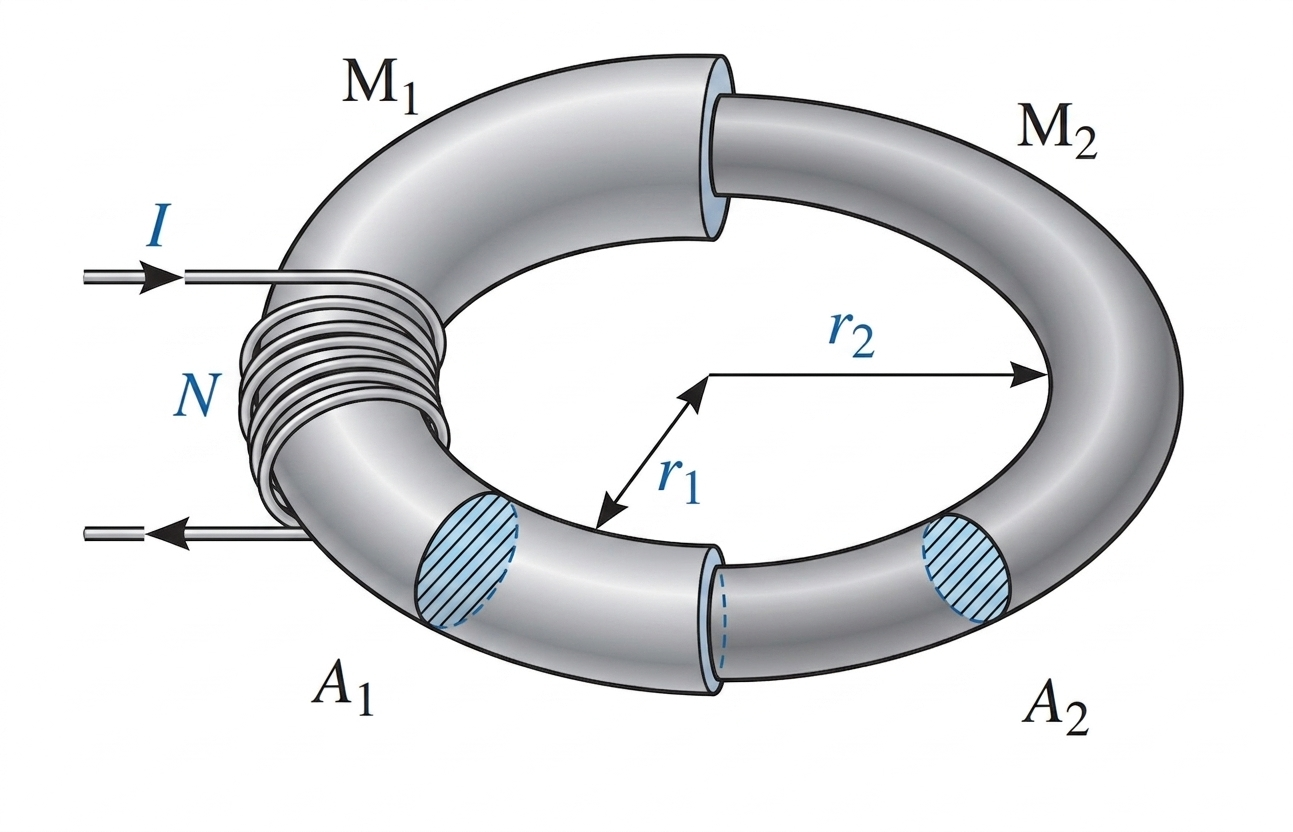
\includegraphics[height=0.3\textheight, width=0.6\textwidth,keepaspectratio]{images/Mcircuit8.png}
\end{center}
\mk{20} \yr{EEE 163 | L-1/T-1 | 2020--21}

\item Find the magnetic flux $\Phi$ for the series magnetic circuit below for the specified impressed mmf.
\begin{center}
      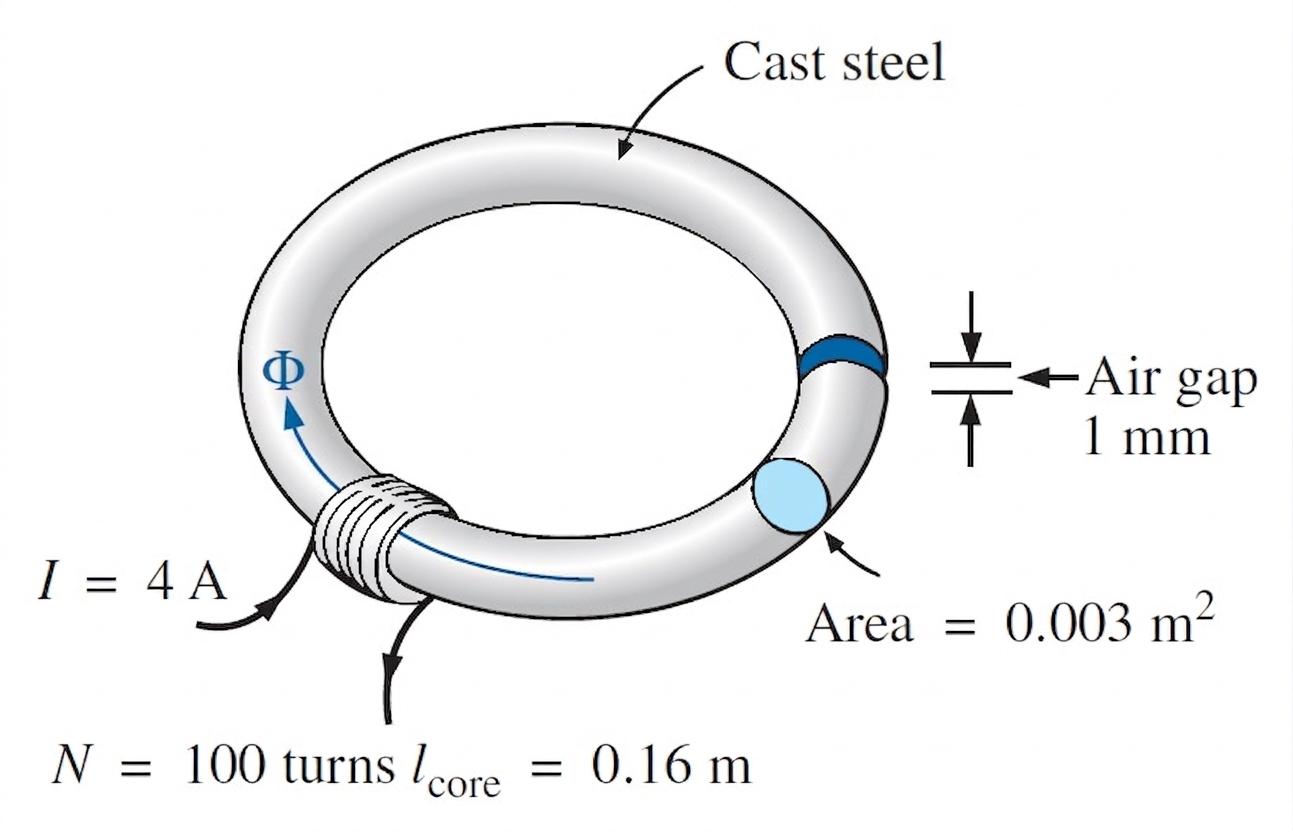
\includegraphics[height=0.3\textheight, width=0.75\textwidth,keepaspectratio]{images/Mcircuit7.png}
\end{center}
\mk{15} \yr{EEE 163 | L-1/T-1 | 2020--21}
\begin{center}
      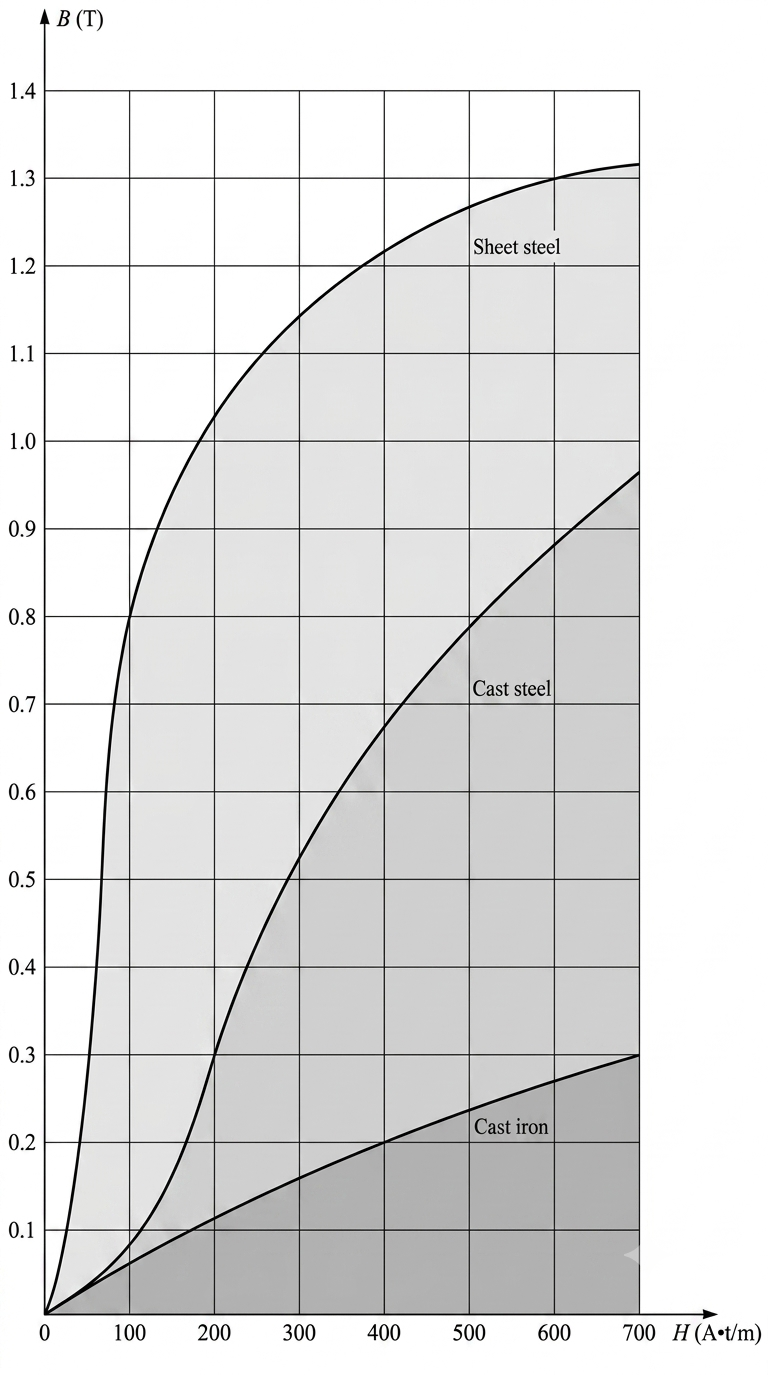
\includegraphics[height=0.6\textheight, width=0.75\textwidth,keepaspectratio]{images/B-H.png}
\end{center}
\[
\textbf{B-H curve for Ques 1 and 2}
\]


\item Determine the value of current $I$ required to establish a flux of $5\times10^{-5}$\,Wb in the cast iron core shown below. (Use magnetic circuit converted to equivalent electrical one.)
\begin{center}
      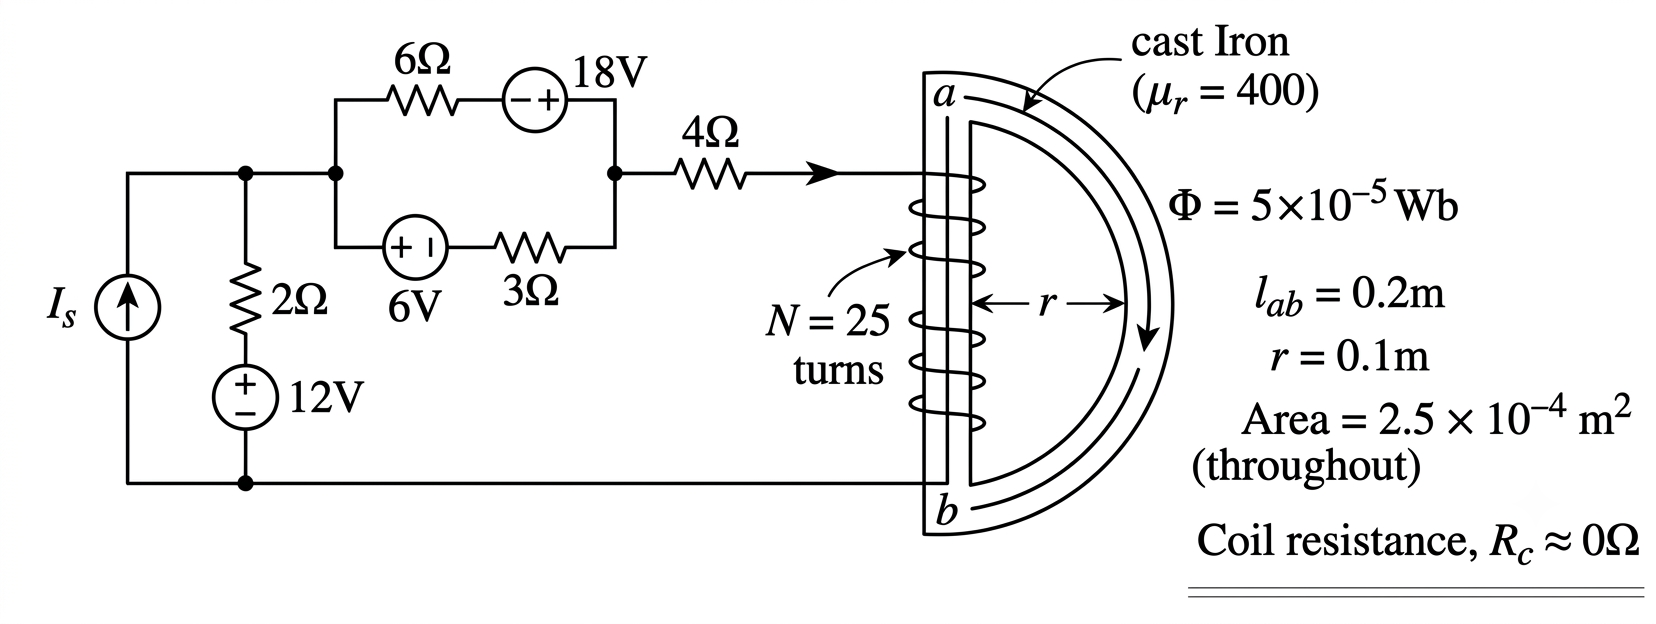
\includegraphics[height=0.3\textheight, width=0.75\textwidth,keepaspectratio]{images/Mcircuit9.png}
\end{center}
\mk{20} \yr{EEE 163 | L-1/T-1 | 2014--15}

\item Find the current $I$ necessary to establish a flux of $\phi = 0.8\times10^{-4}$\,Wb in the series magnetic circuit shown below. Also find the permeability of each material. (Use B--H curve attached.)
\begin{center}
      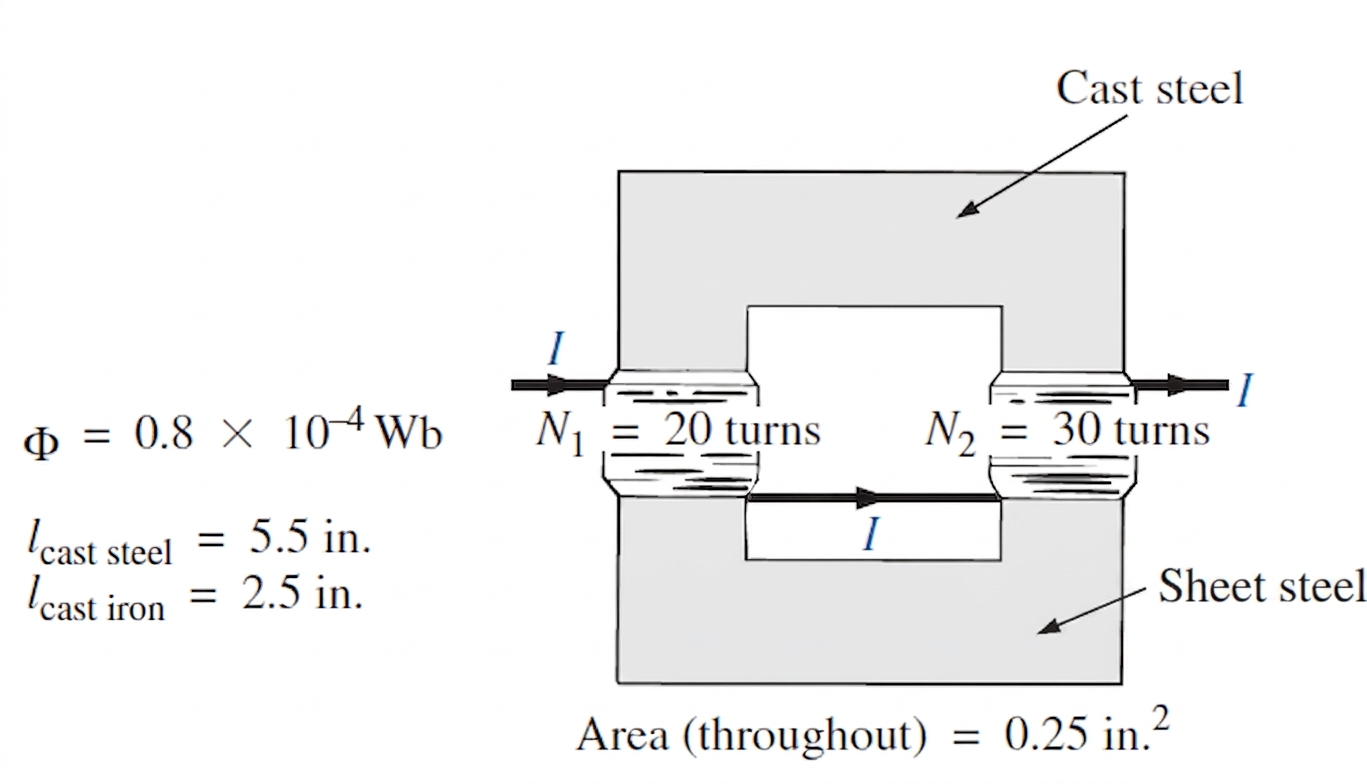
\includegraphics[height=0.3\textheight, width=0.75\textwidth,keepaspectratio]{images/Mcircuit10.png}
      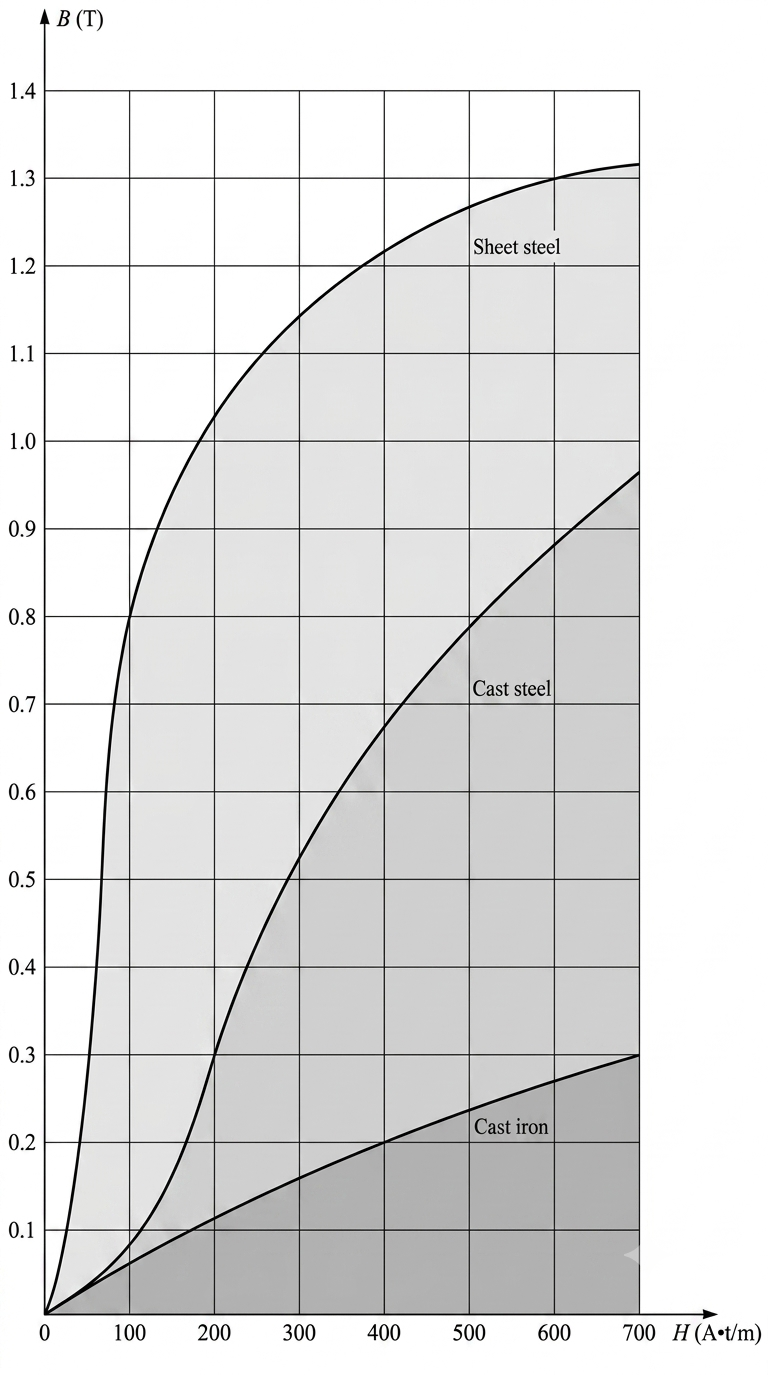
\includegraphics[height=0.6\textheight, width=0.75\textwidth,keepaspectratio]{images/B-H.png}
\end{center}
\mk{20} \yr{EEE 163 | L-1/T-1 | 2014--15}

\item Determine the secondary current $I_2$ for the transformer in the circuit below if the resultant clockwise flux in the core is $1.5\times10^{-5}$\,Wb. (B--H curves for Sheet steel and Cast steel are provided.)
\begin{center}
      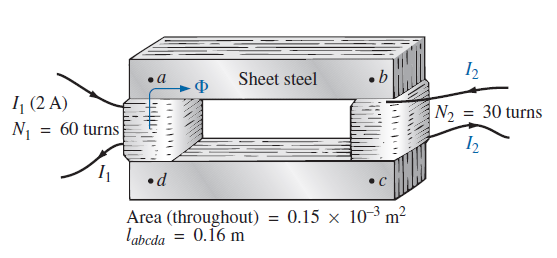
\includegraphics[height=0.3\textheight, width=0.75\textwidth,keepaspectratio]{images/Mcircuit4.png}
\end{center}
\mk{18} \yr{EEE 163 | L-1/T-1 | 2013--14}

\item Find the current $I$ required to establish a flux $\phi = 2.4\times10^{-4}$\,Wb in the circuit below. (B--H curve provided.)
\begin{center}
      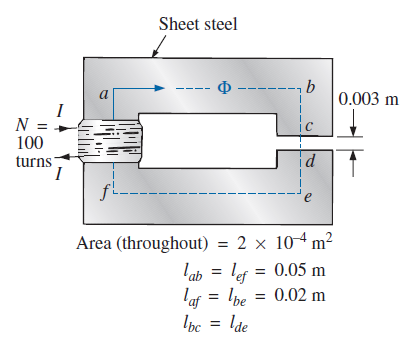
\includegraphics[height=0.3\textheight, width=0.75\textwidth,keepaspectratio]{images/Mcircuit5.png}
      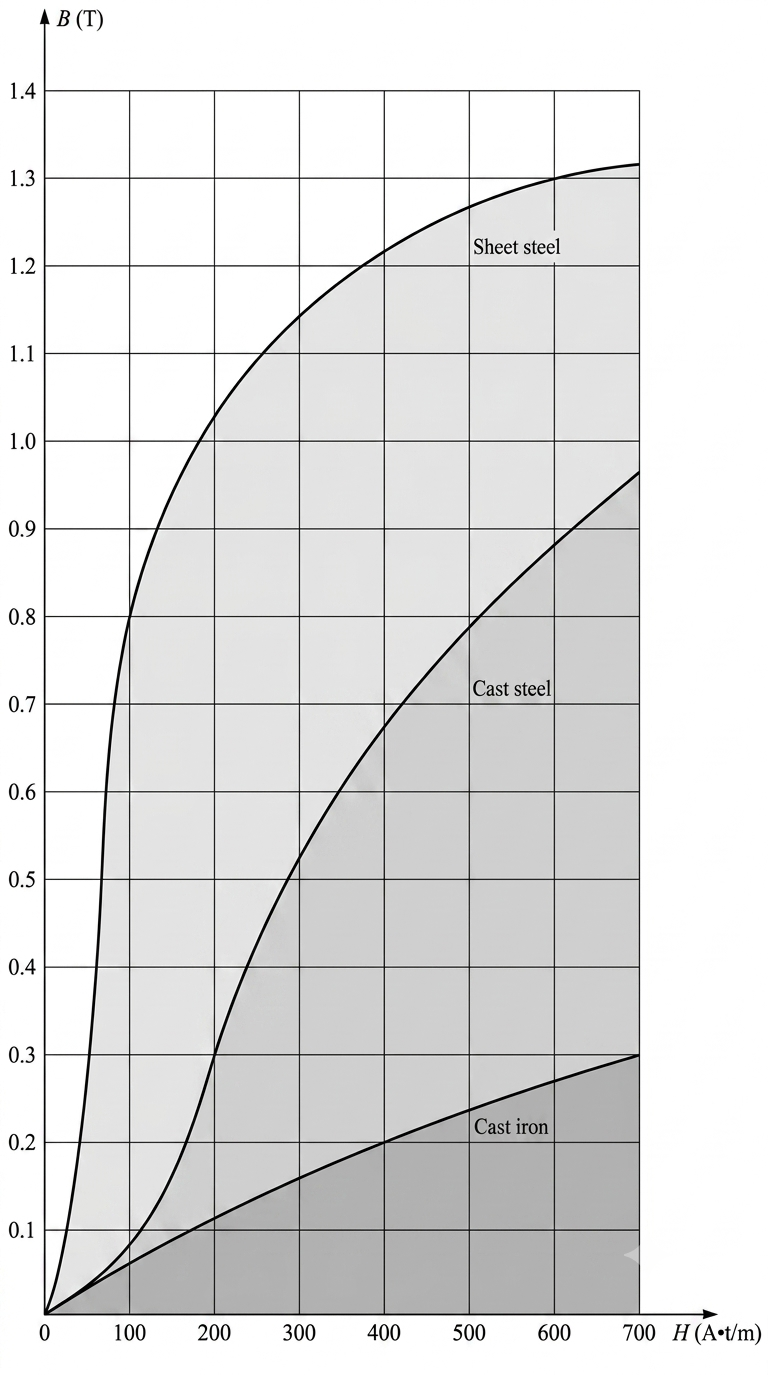
\includegraphics[height=0.6\textheight, width=0.75\textwidth,keepaspectratio]{images/B-H.png}
\end{center}
\[
\textbf{B-H curve for Ques No. 5 \& 6}
\]
\mk{13} \yr{EEE 163 | L-1/T-1 | 2013--14}

\item Draw the equivalent magnetic circuit for the magnetic circuit shown below. Determine $I$ in the same circuit.

\begin{center}
    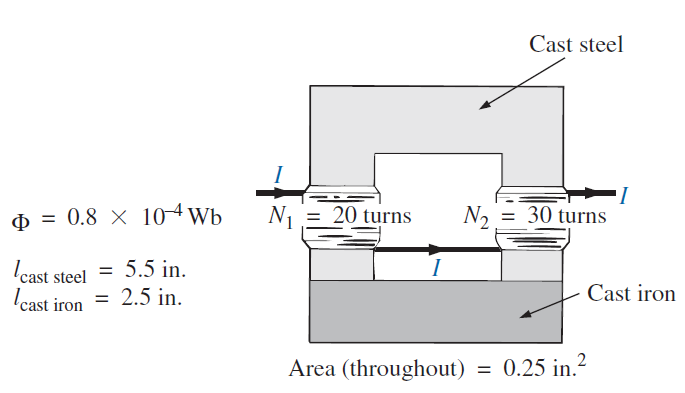
\includegraphics[height=0.3\textheight, width=0.75\textwidth,keepaspectratio]{images/Mcircuit2.png}
\end{center}

\mk{10} \yr{EEE 163 | L-1/T-1 | 2012--13}

\item Determine the magnetic flux $\Phi$ established in the series magnetic circuit shown below.
\begin{center}
    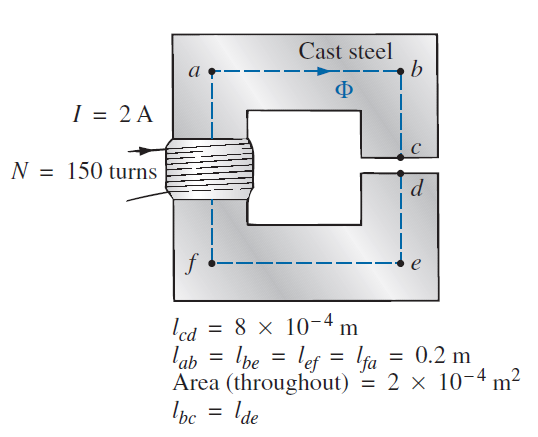
\includegraphics[height=0.3\textheight, width=0.75\textwidth,keepaspectratio]{images/Mcircuit3.png}
\end{center}
\mk{10} \yr{EEE 163 | L-1/T-1 | 2012--13}

\item For the series-parallel magnetic circuit below, find the value of $I$ required to establish a flux in the gap of $\phi_g = 2\times10^{-4}$\,Wb. (B--H curve for different material is given in the figure.)
\begin{center}

  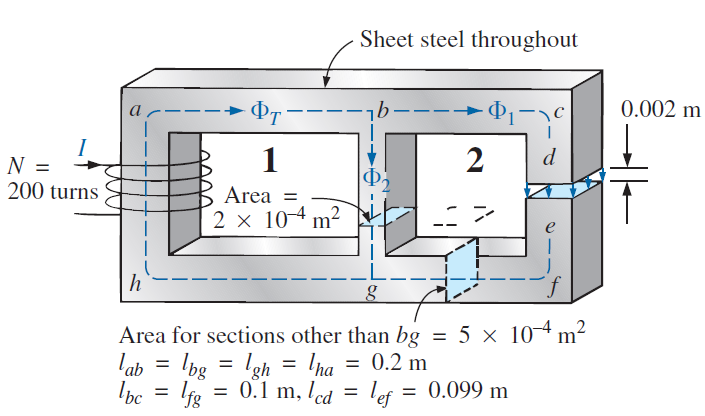
\includegraphics[height=0.3\textheight, width=0.75\textwidth,keepaspectratio]{images/Mcircuit1.png}
\end{center}

\begin{center}
  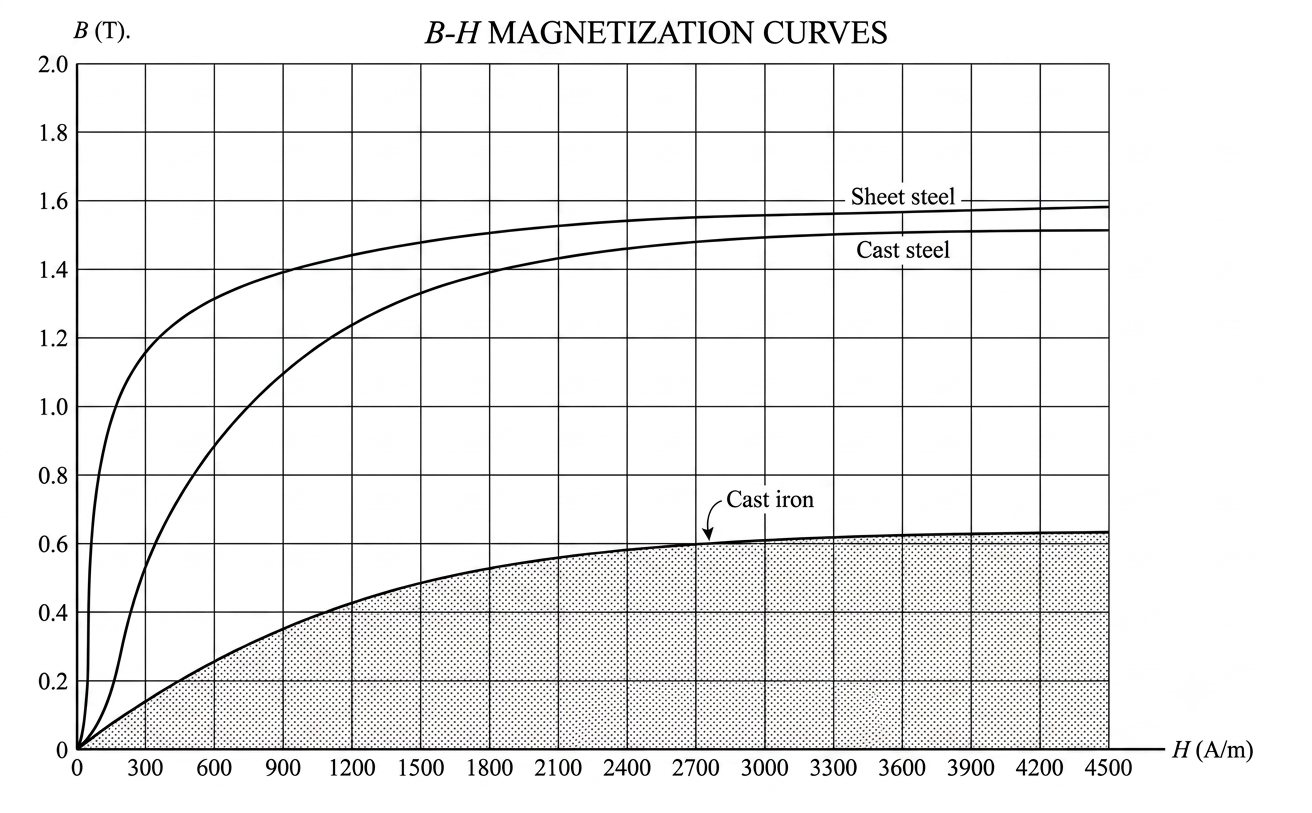
\includegraphics[height=0.5\textheight, width=0.75\textwidth,keepaspectratio]{images/B-Hcurve.png}
\end{center}
\[
\textbf{B-H curve of Ques No. 8 \& 9}
\]
\mk{25} \yr{EEE 163 | L-1/T-1 | 2011--12}

\item Determine the current $I$ required to establish a flux of $\phi_2 = 2\times10^{-4}$\,Wb in the section of the core indicated below.

\begin{center}
    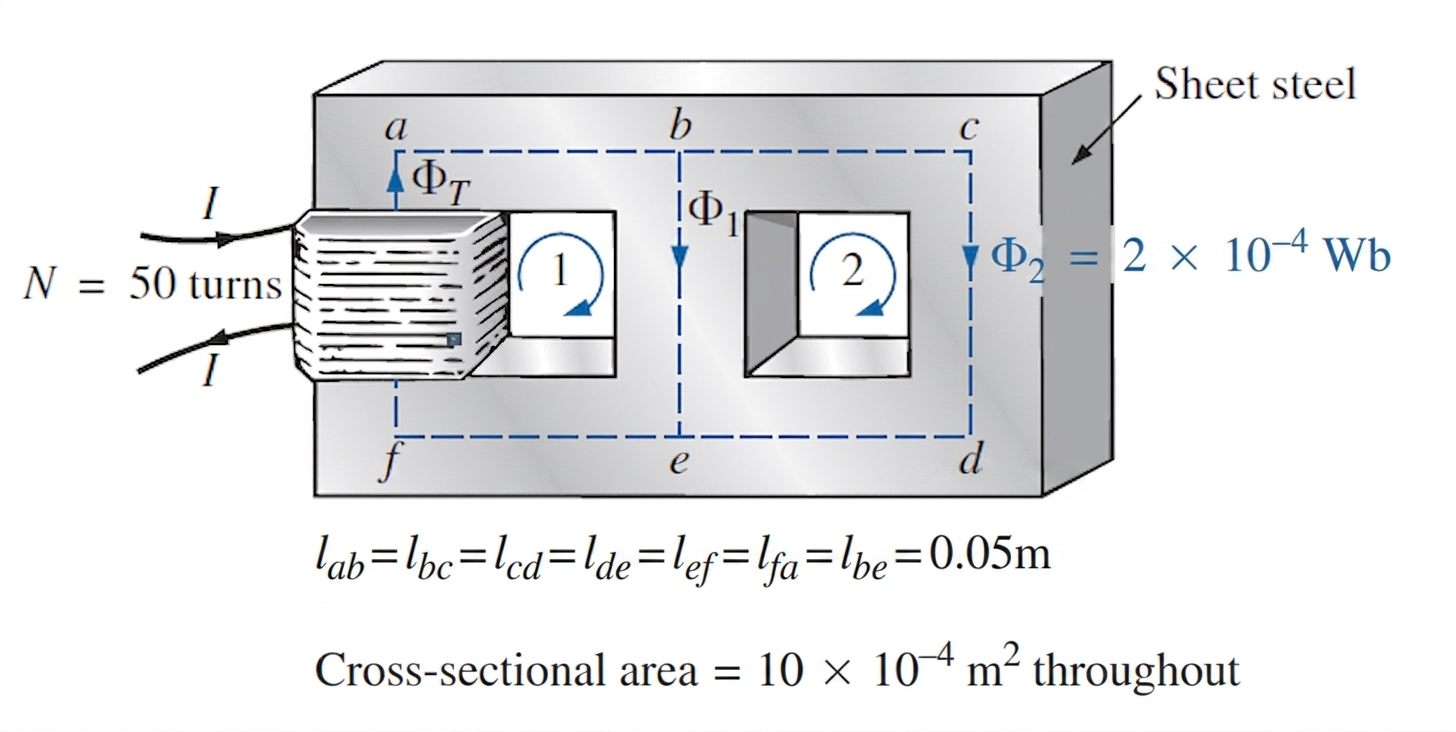
\includegraphics[height=0.5\textheight, width=0.75\textwidth,keepaspectratio]{images/Mcircuit12.png}

  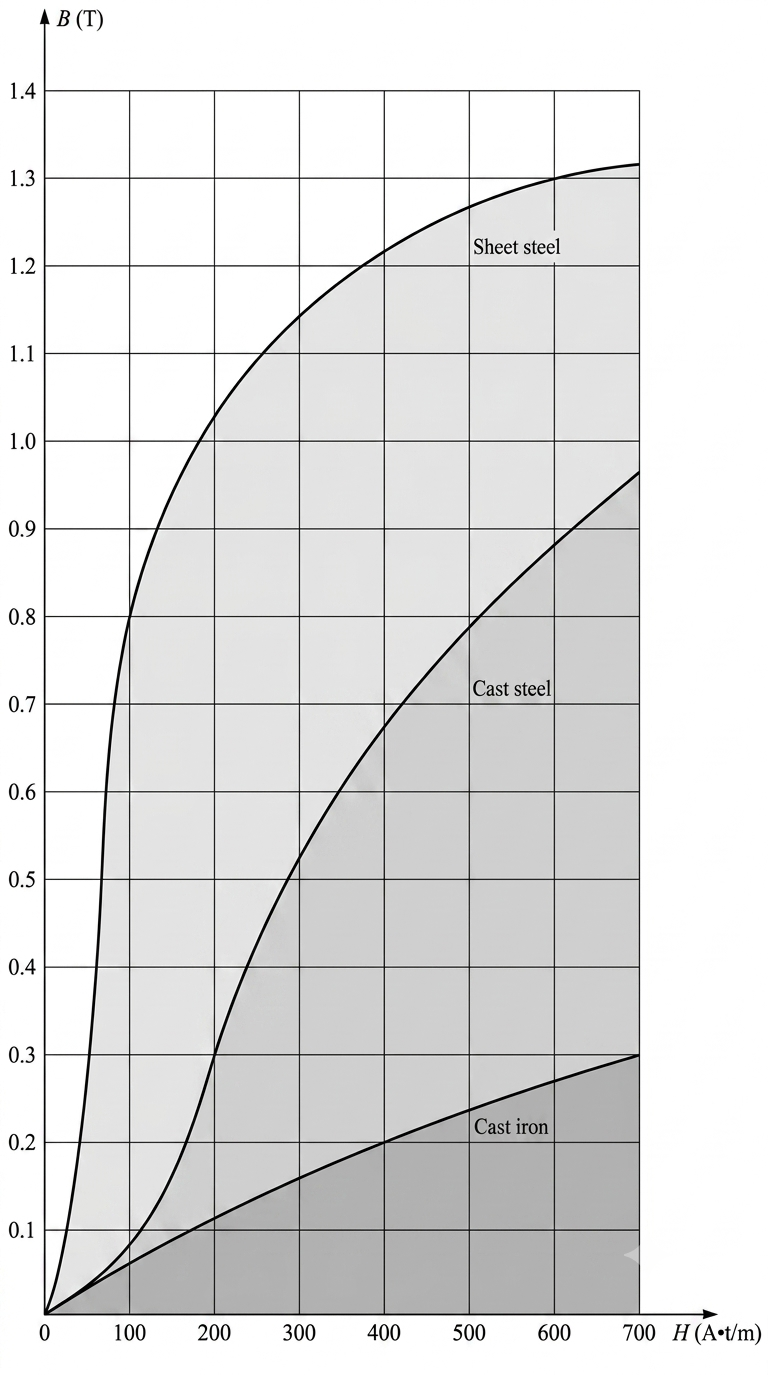
\includegraphics[height=0.5\textheight, width=0.75\textwidth,keepaspectratio]{images/B-H.png}
\end{center}

\mk{20} \yr{EEE 163 | L-1/T-1 | 2010--11}

\item Find the magnetomotive force that produces a total flux of $1.2\times10^{-3}$\,Wb in the following magnetic circuit. Use the attached B--H curves.
\begin{center}
  \begin{tikzpicture}[scale=1.1, >=stealth]

    % Define the 3D depth vector for the oblique projection
    \coordinate (D) at (1.4, 0.9);
    
    % --- 1. Laminated Sheet Steel Base (Bottom Section) ---
    % Front Face of the base
    \draw[thick, fill=white] (0,0) rectangle (6,1);
    
    % Right Side Face of the base (with lamination lines)
    \draw[thick, fill=white] (6,0) -- ++(D) -- ++(0,1) -- (6,1) -- cycle;
    
    % Drawing the vertical lamination hatching lines on the right face
    \foreach \step in {0.08, 0.16, 0.24, 0.32, 0.40, 0.48, 0.56, 0.64, 0.72, 0.80, 0.88, 0.96, 1.04, 1.12, 1.20, 1.28, 1.36} {
        \draw[thin] ($(6,0) + \step*(1, 0.9/1.4)$) -- ($(6,1) + \step*(1, 0.9/1.4)$);
    }
    
    % --- 2. Inner Window Recess (Back & Bottom Interior Surfaces) ---
    \draw[thick, gray!80!black] ($(1,1)+(D)$) -- ($(5,1)+(D)$) -- ($(5,5)+(D)$);
    \draw[thick, gray!80!black] (1,1) -- ($(1,1)+(D)$);
    \draw[thick, gray!80!black] (5,1) -- ($(5,1)+(D)$);
    
    % --- 3. Cast Steel Upper Structure ---
    % Front Face (Two side limbs and the top yoke, leaving the center window open)
    \draw[thick, fill=white, fill opacity=0.7] 
        (0,1) -- (1,1) -- (1,5) -- (5,5) -- (5,1) -- (6,1) -- (6,6) -- (0,6) -- cycle;
    
    % Top Face of the core
    \draw[thick, fill=white] (0,6) -- (6,6) -- ($(6,6)+(D)$) -- ($(0,6)+(D)$) -- cycle;
    
    % Outer Right Face of the upper core
    \draw[thick, fill=white] (6,1) -- (6,6) -- ($(6,6)+(D)$) -- ($(6,1)+(D)$) -- cycle;
    
    % --- 4. Dimensions & Extensions ---
    % Left side heights (2.5 cm and 12.5 cm)
    \draw[<->] (-0.5,0) -- (-0.5,1) node[midway, left] {$2.5\text{ cm}$};
    \draw[<->] (-0.5,1) -- (-0.5,6) node[midway, left] {$12.5\text{ cm}$};
    \draw[thin, dashed] (0,0) -- (-0.6,0);
    \draw[thin, dashed] (0,1) -- (-0.6,1);
    \draw[thin, dashed] (0,6) -- (-0.6,6);
    
    % Bottom total width (15 cm)
    \draw[<->] (0,-0.5) -- (6,-0.5) node[midway, below] {$15\text{ cm}$};
    \draw[thin, dashed] (0,0) -- (0,-0.6);
    \draw[thin, dashed] (6,0) -- (6,-0.6);
    
    % Inner window width (10 cm)
    \draw[<->] (1,3) -- (5,3) node[midway, fill=white, inner sep=2pt] {$10\text{ cm}$};
    
    % Depth thickness (4 cm)
    \draw[<->] ($(6,-0.2)$) -- ($(6,-0.2)+(D)$) node[midway, below right] {$4\text{ cm}$};
    \draw[thin, dashed] (6,0) -- ($(6,0)+(0,-0.2)$);
    \draw[thin, dashed] ($(6,0)+(D)$) -- ($(6,0)+(D)+(0,-0.2)$);
    
    % Top-right yoke thickness (2.5 cm)
    \draw[thin, dashed] ($(6,6)+(D)$) -- ++(1,0) coordinate (H1);
    \draw[thin, dashed] ($(6,5)+(D)$) -- ++(1,0) coordinate (H2);
    \draw[<->] ($(H1)+(0.2,0)$) -- ($(H2)+(0.2,0)$) node[midway, right] {$2.5\text{ cm}$};
    
    % --- 5. Labels & Arrows ---
    % Cast steel label
    \draw[->, thick] (7.8, 4.2) node[right] {Cast steel} -- (5.6, 3.8);
    
    % Lamination label
    \draw[->, thick] (7.8, 2.0) node[right] {lamination} -- ($(6, 0.4) + 0.4*(D)$);
    
    % Laminated sheet steel label
    \draw[->, thick] (5.5, -1.3) node[right] {laminated sheet steel} .. controls (4.5,-1.3) and (3.8,-0.5) .. (3.5, 0.4);
    

\end{tikzpicture}

\end{center}
\begin{center}
  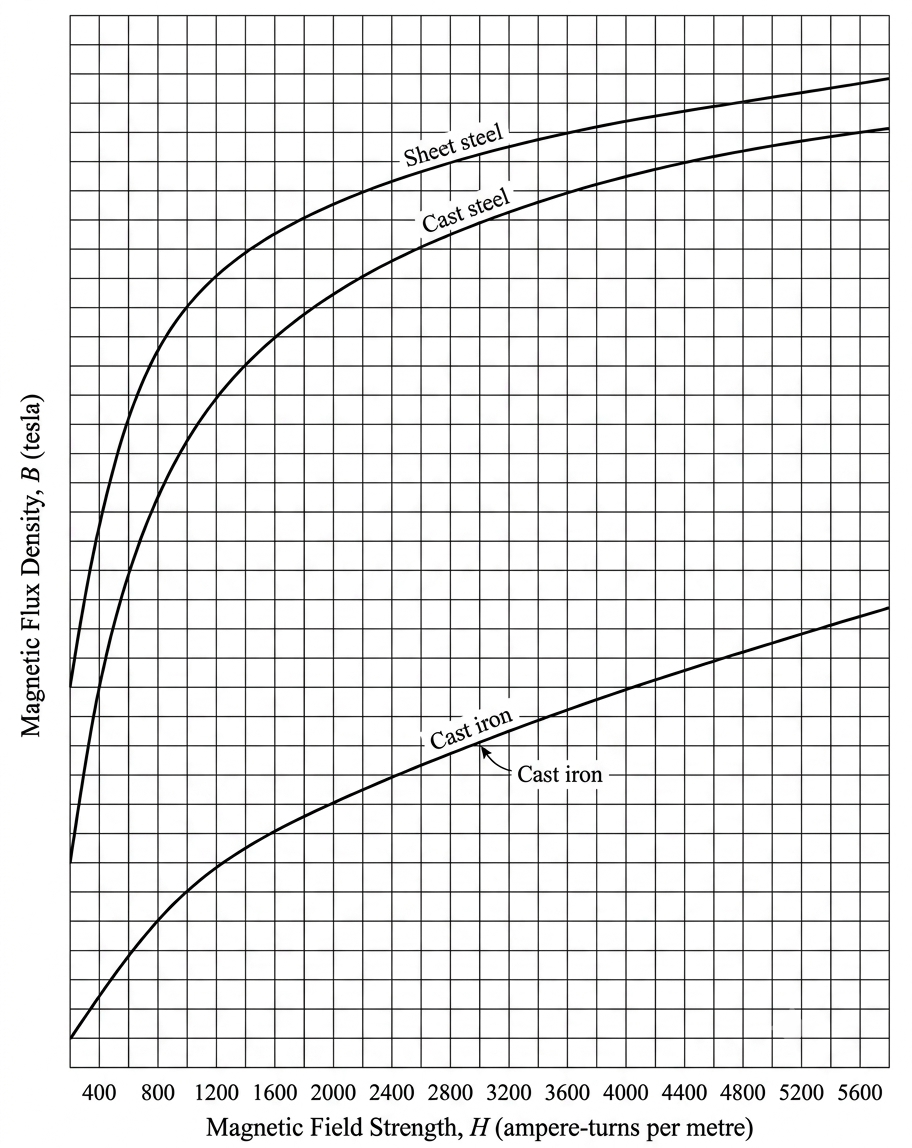
\includegraphics[height=0.5\textheight, width=0.75\textwidth,keepaspectratio]{images/B-Hcurve3.png}
\end{center}
\mk{20} \yr{EEE 163 | L-1/T-1 | 2008--09}

\item A mild steel ring having a cross-sectional area of 500\,mm² and a mean circumference of 400\,mm has a coil of 200 turns wound uniformly around it. To produce a flux of 800\,$\mu$Wb in the ring, calculate: (i)~the reluctance of the ring; (ii)~the current required. (Given that $\mu_r \approx 380$.)
\mk{10} \yr{EEE 163 | L-1/T-1 | 2007--08}

\item A magnetic circuit is made of sheet steel arranged as below. The centre limb is wound with 500 turns. Each of the outer limbs has a cross-sectional area of 300\,mm²; the centre limb has a cross-sectional area of 1000\,mm². The air gap has a length of 1\,mm. Calculate the current required to set up a flux of 1.3\,mWb in the centre limb, assuming no magnetic leakage and fringing. (Use the given B--H curves.)

\begin{center}
\begin{tikzpicture}[xscale=1.2, yscale=1.2, line width=0.8pt]

    % 1. Core Boundaries
    % Outer boundary of the core
    \draw (0,0) rectangle (8,6);

    % Inner boundary (creates the core shape with the 1mm air gap at the top of the central limb)
    \draw (1.5, 1.5) -- (3, 1.5) -- (3, 4.3) -- (5, 4.3) -- (5, 1.5) -- (6.5, 1.5) -- (6.5, 4.5) -- (1.5, 4.5) -- cycle;

    % 2. Mean Flux Path (Dashed Lines)
    % Outer rectangular loop with rounded corners
    \draw[dashed, rounded corners=10pt] (0.75, 0.75) rectangle (7.25, 5.25);
    % Central limb flux path
    \draw[dashed] (4, 0.75) -- (4, 5.25);

    % Flux directional arrows at the junctions (mimicking the hand sketch)
    % Top junction arrows pointing inwards/downwards
    \draw[-stealth] (3.7, 5.25) -- (3.95, 5.05); 
    \draw[-stealth] (4.3, 5.25) -- (4.05, 5.05);
    
    % Bottom junction arrows pointing inwards/upwards
    \draw[-stealth] (3.7, 0.75) -- (3.95, 0.95);
    \draw[-stealth] (4.3, 0.75) -- (4.05, 0.95);

    % 3. Coil
    % Entry wire (Top left)
    \draw (1.5, 3.5) -- (3, 3.5);
    \draw[-stealth] (1.5, 3.5) -- (2.4, 3.5) node[midway, above] {$I$};
    
    % Coil loops (Simulating 3D wrapping around the central limb)
    \draw (3, 3.5) to[out=-10, in=190] (5, 3.3);             % Front cross 1
    \draw (5, 3.3) to[out=10, in=90] (5.2, 3.15);            % Right wrap around 1
    
    \draw (2.8, 3.15) to[out=-90, in=170] (3, 3.0);          % Left emergence 1
    \draw (3, 3.0) to[out=-10, in=190] (5, 2.8);             % Front cross 2
    \draw (5, 2.8) to[out=10, in=90] (5.2, 2.65);            % Right wrap around 2
    
    \draw (2.8, 2.65) to[out=-90, in=170] (3, 2.5);          % Left emergence 2
    \draw (3, 2.5) to[out=-10, in=190] (5, 2.3);             % Front cross 3
    \draw (5, 2.3) to[out=10, in=90] (5.2, 2.15);            % Right wrap around 3
    
    \draw (2.8, 2.15) to[out=-90, in=170] (3, 2.0);          % Left emergence 3
    
    % Exit wire (Bottom left)
    \draw (3, 2.0) -- (1.5, 2.0);
    \draw[-stealth] (3, 2.0) -- (2.1, 2.0);

    % 4. Dimension Labels
    % Left height label
    \node[left, align=center] at (-0.2, 3) {300 \\ mm};
    
    % Right height label
    \node[right, align=center] at (8.2, 3) {300 \\ mm};
    
    % Central limb width label
    \draw[stealth-stealth] (3, 1.0) -- (5, 1.0) node[midway, fill=white, inner sep=2pt] {120 mm};
    
    % Air gap label
    \draw[-stealth] (5.8, 4.4) -- (5.1, 4.4);
    \node[right] at (5.8, 4.4) {1 mm};

\end{tikzpicture}
\end{center}

\mk{15} \yr{EEE 163 | L-1/T-1 | 2007--08}

\item For the series-parallel magnetic circuit shown below, find the value of $I$ required to establish a flux in the gap, $\phi_g = 2\times10^{-4}\,\text{Wb}$.
\begin{center}
  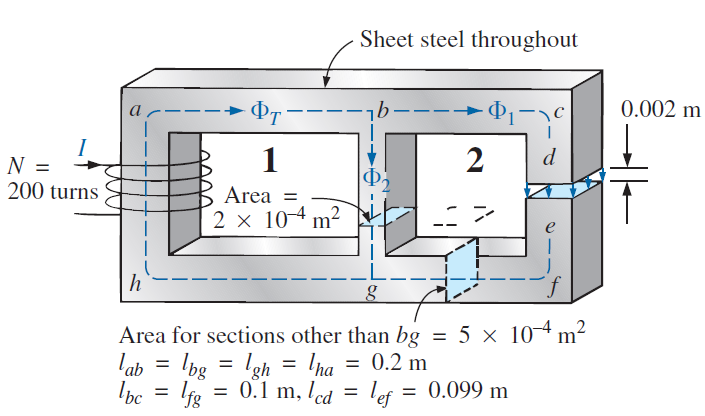
\includegraphics[height=0.5\textheight, width=0.75\textwidth,keepaspectratio]{images/Mcircuit1.png}
    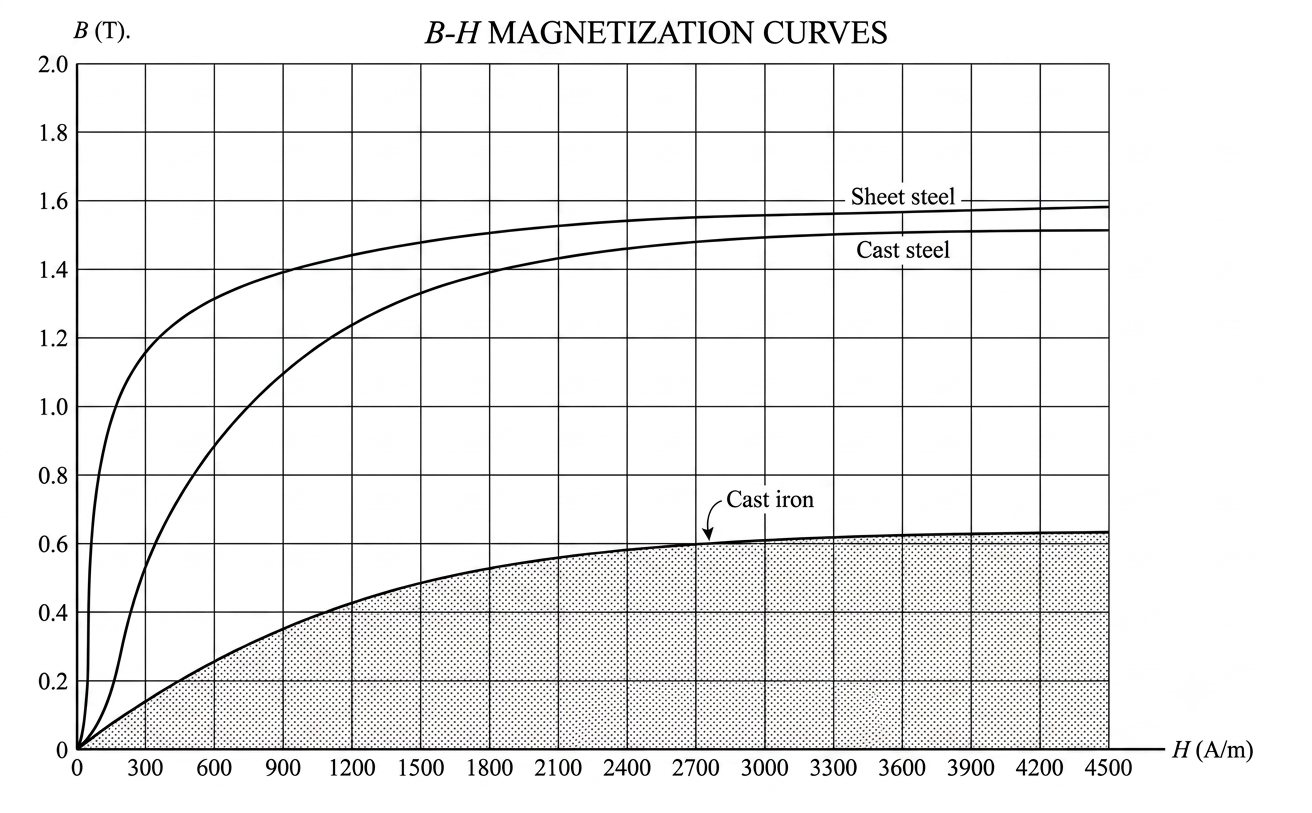
\includegraphics[height=0.6\textheight, width=0.75\textwidth,keepaspectratio]{images/B-Hcurve.png}
\end{center}
\[
\textbf{B-H curve for Ques No. 13 \& 14}
\]
\mk{17} \yr{EEE 163 | L-1/T-1 | 2006--07}

\item The ferrite core drawn below has a rectangular cross-section with height 0.025\,inch. Its inner and outer diameters are 0.05\,inch and 0.08\,inch respectively. Flux density inside the core is 0.15\,Tesla. The core material has relative permeability $\mu_r = 1000$. Determine the Ampere-turns and reluctance of this magnetic circuit.
\begin{center}
  

\begin{tikzpicture}[>=stealth]

    % --- 1. Back Wires (Core-er pechone thakbe) ---
    \foreach \angle in {30, 60, 90, 120, 150, 180, 210, 240, 270, 300} {
        \draw[thick, gray!80] (\angle:1.4) -- (\angle+15:2.2);
    }

    % --- 2. Toroid Core (Shaded with Even-Odd Rule to cover back wires) ---
    \draw[thick, fill=gray!20, even odd rule] (0,0) circle (1.4) (0,0) circle (2.2);
    
    % Core Center Dot (Optional, for reference)
    \fill (0,0) circle (1.5pt);

    % --- 3. Front Wires (Core-er upor diye pechano) ---
    % Arrow decoration for current direction on the front loops
    \begin{scope}[decoration={markings, mark=at position 0.55 with {\arrow{>}}}]
        
        % First incoming wire from bottom right
        \draw[thick, postaction={decorate}] (2.5, -0.7) -- (30:2.2);
        \node[below] at (2.5, -0.7) {$I$};
        
        % Winding loops across the front face
        \draw[thick, postaction={decorate}] (30:2.2)  .. controls (35:2.3)  and (55:1.5)  .. (60:1.4);
        \draw[thick, postaction={decorate}] (60:2.2)  .. controls (65:2.3)  and (85:1.5)  .. (90:1.4);
        \draw[thick, postaction={decorate}] (90:2.2)  .. controls (95:2.3)  and (115:1.5) .. (120:1.4);
        \draw[thick, postaction={decorate}] (120:2.2) .. controls (125:2.3) and (145:1.5) .. (150:1.4);
        \draw[thick, postaction={decorate}] (150:2.2) .. controls (155:2.3) and (175:1.5) .. (180:1.4);
        \draw[thick, postaction={decorate}] (180:2.2) .. controls (185:2.3) and (205:1.5) .. (210:1.4);
        \draw[thick, postaction={decorate}] (210:2.2) .. controls (215:2.3) and (235:1.5) .. (240:1.4);
        \draw[thick, postaction={decorate}] (240:2.2) .. controls (245:2.3) and (265:1.5) .. (270:1.4);
        \draw[thick, postaction={decorate}] (270:2.2) .. controls (275:2.3) and (295:1.5) .. (300:1.4);
        \draw[thick, postaction={decorate}] (300:2.2) .. controls (305:2.3) and (325:1.5) .. (330:1.4);
        
        % Last outgoing wire to top right
        \draw[thick, postaction={decorate}] (330:1.4) -- (2.5, 0.7);
        
    \end{scope}

    % --- 4. Labels and Dimensions ---
    % Label for Number of turns
    \node at (2.7, 0.6) {$N$};
    
    % Dashed lines to show mean radius or dimensions if needed
    \draw[dashed, ->] (0,0) -- (45:1.4) node[midway, above left=-2pt] {$r_1$};
    \draw[dashed, ->] (0,0) -- (15:2.2) node[midway, above] {$r_2$};
% --- Figure Caption ---

\end{tikzpicture}
\end{center}
\mk{20} \yr{EEE 163 | L-1/T-1 | 2005--06}

\end{enumerate}

%%──────────────────────────────────────────────────────────────────────
\subtopic{cD}{Hysteresis \& Magnetic Properties}
\label{sub:s5-hysteresis}

\begin{enumerate}\item Derive $B = \mu H$ [symbols have usual meanings]. Explain the set-up used to develop a B--H curve for a material and hence explain the different parts of the curve.
\mk{15} \yr{EEE 163 | L-1/T-1 | 2012--13}

\item Briefly explain the hysteresis curve.
\mk{10} \yr{EEE 163 | L-1/T-1 | 2011--12}

\item Define: MMF, Magnetic flux density and permeability.
\mk{9} \yr{EEE 163 | L-1/T-1 | 2010--11}

\item State Ampere's circuit law.
\mk{6} \yr{EEE 163 | L-1/T-1 | 2010--11}

\item Write short notes on: 
\begin{enumerate}
  \item Hysteresis
  \item Power factor correction
  \item Similarities and dissimilarities between electric circuits and magnetic circuits
  \item Power generation and distribution in Bangladesh
  \item Loadshedding and daylight saving.
\end{enumerate}
\mk{7} \yr{EEE 163 | L-1/T-1 | 2008--09}

\item Write short notes on: Similarities and dissimilarities between electric circuits and magnetic circuits.
\mk{7} \yr{EEE 163 | L-1/T-1 | 2008--09}

\item How are magnetic flux lines established around a current-carrying conductor?
\mk{5} \yr{EEE 163 | L-1/T-1 | 2007--08}

\item Define permeability. Can we apply the superposition principle to a magnetic circuit? Give reasons to support your answer.
\mk{5} \yr{EEE 163 | L-1/T-1 | 2007--08}

\item State Ampere's Circuit Law and Ohm's Law for magnetic circuit.
\mk{3+2} \yr{EEE 163 | L-1/T-1 | 2006--07}

\item Draw the hysteresis curves when the maximum value of $H$ is:
\begin{enumerate}
  \item Greater than the saturation value.
  \item Less than the saturation value.
\end{enumerate}
Also explain the reasons behind the shape of the hysteresis curves.
\mk{3+3+7} \yr{EEE 163 | L-1/T-1 | 2006--07}

\end{enumerate}


%% ══════════════════════════════════════════════════════════════════════
%%  PART VI — MISCELLANEOUS
%% ══════════════════════════════════════════════════════════════════════
\secdivider{Part VI --- Miscellaneous \& Short Notes}{General EEE Topics, Power Generation \& Distribution}{cF}

\markboth{S6: Miscellaneous}{S6: Miscellaneous}
\label{sec:S6}
\titleformat{\section}{\large\bfseries\color{cF}}{}{0em}{}[\titlerule]
\section*{S6 \quad Miscellaneous \& Short Notes}
\addcontentsline{toc}{section}{S6: Miscellaneous \& Short Notes}

%%──────────────────────────────────────────────────────────────────────
\subtopic{cF}{Short Notes}
\label{sub:s6-shortnotes}

\begin{enumerate}\item Write short notes on: Power generation and distribution in Bangladesh.
\mk{7} \yr{EEE 163 | L-1/T-1 | 2008--09}

\item Write short notes on: Loadshedding and daylight saving.
\mk{7} \yr{EEE 163 | L-1/T-1 | 2008--09}

\end{enumerate}

\end{document}